%% Adaptado a partir de :
%DIF LATEXDIFF DIFFERENCE FILE
%DIF DEL versao_antiga/main-texto-completo.tex   Fri Mar 10 00:08:11 2023
%DIF ADD versao_nova/main-texto-completo.tex     Fri Mar 10 00:37:03 2023
%%    abtex2-modelo-trabalho-academico.tex, v-1.9.2 laurocesar
%% para ser um modelo para os trabalhos no IFSP-SPO

\documentclass[
    % -- opções da classe memoir --
    12pt,               % tamanho da fonte
    openright,          % capítulos começam em pág ímpar (insere página vazia caso preciso)
    %twoside,            % para impressão em verso e anverso. Oposto a oneside
    oneside,
    a4paper,            % tamanho do papel. 
    BIBLATEX,           % indica para utilizar BIBLATEX em vez do abntex2cite
    % -- opções da classe abntex2 --
    %chapter=TITLE,     % títulos de capítulos convertidos em letras maiúsculas
    %section=TITLE,     % títulos de seções convertidos em letras maiúsculas
    %subsection=TITLE,  % títulos de subseções convertidos em letras maiúsculas
    %subsubsection=TITLE,% títulos de subsubseções convertidos em letras maiúsculas
    % Opções que não devem ser utilizadas na versão final do documento
    %draft,              % para compilar mais rápido, remover na versão final
%   MODELO,             % indica que é um documento modelo então precisa dos geradores de texto
    TODO,               % indica que deve apresentar lista de pendencias 
    % -- opções do pacote babel --
    english,            % idioma adicional para hifenização
    brazil              % o último idioma é o principal do documento
    ]{ifsp-spo-inf-ctds}
    
        
% ---

% --- 
% CONFIGURAÇÕES DE PACOTES
% --- 
%\usepackage{etoolbox}
%\patchcmd{\thebibliography}{\chapter*}{\section*}{}{}
\usepackage{svg} 
\usepackage{tabulary}
\usepackage{graphicx}
\graphicspath{ {./images/} }
\setlength {\marginparwidth }{2cm} 
\usepackage{float}
% carregando aqui referencias quando utilizando BIBLATEX
\IfPackageLoaded{biblatex}{%
\addbibresource{referencias.bib}
\addbibresource{exemplos/abntex2-doc-abnt-6023.bib}
}{}

% ---
% Informações de dados para CAPA e FOLHA DE ROSTO
% ---
\titulo{CertVet - Gerenciador de clínica veterinária}

% Trabalho individual
%\autor{JOSÉ BRAZ DE ARAUJO}

% Trabalho em Equipe
% ver também https://github.com/abntex/abntex2/wiki/FAQ#como-adicionar-mais-de-um-autor-ao-meu-projeto
\renewcommand{\imprimirautor}{
    \begin{tabular}{lr}
        CAIQUE DANIEL FREITAS EUFRASIO DA SILVA & SP3046711 \\
        HENRIQUE HIROMI SHIMADA                 & SP3039421 \\
        IRINA CHANG GOUVEIA FERREIRA            & SP3058123 \\
        LUIS RENATO MOREIRA DA COSTA            & SP3035531 \\
        MARCOS QUERINO DOS SANTOS E SANTOS JUNIOR & SP3047245 \\
        MURILO SANTOS PIRES                     & SP3052737 \\
%DIF 65d65
%DIF <         WELEN MOTA SOUSA                        & SP146616X
%DIF -------
    \end{tabular}
}


%DIF 70c69
%DIF < \tipotrabalho{Projeto da Disciplina Projeto Integrado I}
%DIF -------
\tipotrabalho{Projeto da Disciplina Projeto Integrado II} %DIF > 
%DIF -------

%DIF 72c71
%DIF < \disciplina{PI1A5 - Projeto Integrado I}
%DIF -------
\disciplina{PI2A6 - Projeto Integrado II} %DIF > 
%DIF -------

%DIF 74c73
%DIF < \preambulo{Trabalho apresentado no curso de Tecnologia em Análise e Desenvolvimento de Sistemas do Instituto Federal de Educação, Ciência e Tecnologia de São Paulo como requisito parcial para a conclusão da disciplina de Projeto Integrado 1}
%DIF -------
\preambulo{Trabalho apresentado no curso de Tecnologia em Análise e Desenvolvimento de Sistemas do Instituto Federal de Educação, Ciência e Tecnologia de São Paulo como requisito parcial para a conclusão da disciplina de Projeto Integrado II} %DIF > 
%DIF -------

%DIF 76c75
%DIF < \data{DEZEMBRO DE 2022}
%DIF -------
\data{MARÇO DE 2023} %DIF > 
%DIF -------

% Definir o que for necessário e comentar o que não for necessário
% Utilizar o Nome Completo, abntex tem orientador e coorientador
% então vão ser utilizados na definição de professor
\renewcommand{\orientadorname}{Professor:}
%DIF 82c81
%DIF < \orientador{ANTONIO AIRTON PALLADINO}
%DIF -------
\orientador{CARLOS HENRIQUE VERISSIMO PEREIRA} %DIF > 
%DIF -------
\renewcommand{\coorientadorname}{Professor:}
\coorientador{JOSÉ BRAZ DE ARAUJO}



% ---


% ---
% Configurações de aparência do PDF final


% informações do PDF
\makeatletter
\hypersetup{
        %pagebackref=true,
        pdftitle={\@title}, 
        pdfauthor={\@author},
        pdfsubject={\imprimirpreambulo},
        pdfcreator={LaTeX with abnTeX2},
        pdfkeywords={abnt}{latex}{abntex}{abntex2}{trabalho acadêmico}, 
        colorlinks=true,            % false: boxed links; true: colored links
        linkcolor=blue,             % color of internal links
        citecolor=blue,             % color of links to bibliography
        filecolor=magenta,              % color of file links
        urlcolor=blue,
        bookmarksdepth=4
}
\makeatother
% --- 

% ---

% ----
% Início do documento
% ----
%DIF PREAMBLE EXTENSION ADDED BY LATEXDIFF
%DIF UNDERLINE PREAMBLE %DIF PREAMBLE
\RequirePackage[normalem]{ulem} %DIF PREAMBLE
\RequirePackage{color}\definecolor{RED}{rgb}{1,0,0}\definecolor{BLUE}{rgb}{0,0,1} %DIF PREAMBLE
\providecommand{\DIFadd}[1]{{\protect\color{blue}\uwave{#1}}} %DIF PREAMBLE
\providecommand{\DIFdel}[1]{{\protect\color{red}\sout{#1}}}                      %DIF PREAMBLE
%DIF SAFE PREAMBLE %DIF PREAMBLE
\providecommand{\DIFaddbegin}{} %DIF PREAMBLE
\providecommand{\DIFaddend}{} %DIF PREAMBLE
\providecommand{\DIFdelbegin}{} %DIF PREAMBLE
\providecommand{\DIFdelend}{} %DIF PREAMBLE
\providecommand{\DIFmodbegin}{} %DIF PREAMBLE
\providecommand{\DIFmodend}{} %DIF PREAMBLE
%DIF FLOATSAFE PREAMBLE %DIF PREAMBLE
\providecommand{\DIFaddFL}[1]{\DIFadd{#1}} %DIF PREAMBLE
\providecommand{\DIFdelFL}[1]{\DIFdel{#1}} %DIF PREAMBLE
\providecommand{\DIFaddbeginFL}{} %DIF PREAMBLE
\providecommand{\DIFaddendFL}{} %DIF PREAMBLE
\providecommand{\DIFdelbeginFL}{} %DIF PREAMBLE
\providecommand{\DIFdelendFL}{} %DIF PREAMBLE
\newcommand{\DIFscaledelfig}{0.5}
%DIF HIGHLIGHTGRAPHICS PREAMBLE %DIF PREAMBLE
\RequirePackage{settobox} %DIF PREAMBLE
\RequirePackage{letltxmacro} %DIF PREAMBLE
\newsavebox{\DIFdelgraphicsbox} %DIF PREAMBLE
\newlength{\DIFdelgraphicswidth} %DIF PREAMBLE
\newlength{\DIFdelgraphicsheight} %DIF PREAMBLE
% store original definition of \includegraphics %DIF PREAMBLE
\LetLtxMacro{\DIFOincludegraphics}{\includegraphics} %DIF PREAMBLE
\newcommand{\DIFaddincludegraphics}[2][]{{\color{blue}\fbox{\DIFOincludegraphics[#1]{#2}}}} %DIF PREAMBLE
\newcommand{\DIFdelincludegraphics}[2][]{% %DIF PREAMBLE
\sbox{\DIFdelgraphicsbox}{\DIFOincludegraphics[#1]{#2}}% %DIF PREAMBLE
\settoboxwidth{\DIFdelgraphicswidth}{\DIFdelgraphicsbox} %DIF PREAMBLE
\settoboxtotalheight{\DIFdelgraphicsheight}{\DIFdelgraphicsbox} %DIF PREAMBLE
\scalebox{\DIFscaledelfig}{% %DIF PREAMBLE
\parbox[b]{\DIFdelgraphicswidth}{\usebox{\DIFdelgraphicsbox}\\[-\baselineskip] \rule{\DIFdelgraphicswidth}{0em}}\llap{\resizebox{\DIFdelgraphicswidth}{\DIFdelgraphicsheight}{% %DIF PREAMBLE
\setlength{\unitlength}{\DIFdelgraphicswidth}% %DIF PREAMBLE
\begin{picture}(1,1)% %DIF PREAMBLE
\thicklines\linethickness{2pt} %DIF PREAMBLE
{\color[rgb]{1,0,0}\put(0,0){\framebox(1,1){}}}% %DIF PREAMBLE
{\color[rgb]{1,0,0}\put(0,0){\line( 1,1){1}}}% %DIF PREAMBLE
{\color[rgb]{1,0,0}\put(0,1){\line(1,-1){1}}}% %DIF PREAMBLE
\end{picture}% %DIF PREAMBLE
}\hspace*{3pt}}} %DIF PREAMBLE
} %DIF PREAMBLE
\LetLtxMacro{\DIFOaddbegin}{\DIFaddbegin} %DIF PREAMBLE
\LetLtxMacro{\DIFOaddend}{\DIFaddend} %DIF PREAMBLE
\LetLtxMacro{\DIFOdelbegin}{\DIFdelbegin} %DIF PREAMBLE
\LetLtxMacro{\DIFOdelend}{\DIFdelend} %DIF PREAMBLE
\DeclareRobustCommand{\DIFaddbegin}{\DIFOaddbegin \let\includegraphics\DIFaddincludegraphics} %DIF PREAMBLE
\DeclareRobustCommand{\DIFaddend}{\DIFOaddend \let\includegraphics\DIFOincludegraphics} %DIF PREAMBLE
\DeclareRobustCommand{\DIFdelbegin}{\DIFOdelbegin \let\includegraphics\DIFdelincludegraphics} %DIF PREAMBLE
\DeclareRobustCommand{\DIFdelend}{\DIFOaddend \let\includegraphics\DIFOincludegraphics} %DIF PREAMBLE
\LetLtxMacro{\DIFOaddbeginFL}{\DIFaddbeginFL} %DIF PREAMBLE
\LetLtxMacro{\DIFOaddendFL}{\DIFaddendFL} %DIF PREAMBLE
\LetLtxMacro{\DIFOdelbeginFL}{\DIFdelbeginFL} %DIF PREAMBLE
\LetLtxMacro{\DIFOdelendFL}{\DIFdelendFL} %DIF PREAMBLE
\DeclareRobustCommand{\DIFaddbeginFL}{\DIFOaddbeginFL \let\includegraphics\DIFaddincludegraphics} %DIF PREAMBLE
\DeclareRobustCommand{\DIFaddendFL}{\DIFOaddendFL \let\includegraphics\DIFOincludegraphics} %DIF PREAMBLE
\DeclareRobustCommand{\DIFdelbeginFL}{\DIFOdelbeginFL \let\includegraphics\DIFdelincludegraphics} %DIF PREAMBLE
\DeclareRobustCommand{\DIFdelendFL}{\DIFOaddendFL \let\includegraphics\DIFOincludegraphics} %DIF PREAMBLE
%DIF LISTINGS PREAMBLE %DIF PREAMBLE
\RequirePackage{listings} %DIF PREAMBLE
\RequirePackage{color} %DIF PREAMBLE
\lstdefinelanguage{DIFcode}{ %DIF PREAMBLE
%DIF DIFCODE_UNDERLINE %DIF PREAMBLE
  moredelim=[il][\color{red}\sout]{\%DIF\ <\ }, %DIF PREAMBLE
  moredelim=[il][\color{blue}\uwave]{\%DIF\ >\ } %DIF PREAMBLE
} %DIF PREAMBLE
\lstdefinestyle{DIFverbatimstyle}{ %DIF PREAMBLE
	language=DIFcode, %DIF PREAMBLE
	basicstyle=\ttfamily, %DIF PREAMBLE
	columns=fullflexible, %DIF PREAMBLE
	keepspaces=true %DIF PREAMBLE
} %DIF PREAMBLE
\lstnewenvironment{DIFverbatim}{\lstset{style=DIFverbatimstyle}}{} %DIF PREAMBLE
\lstnewenvironment{DIFverbatim*}{\lstset{style=DIFverbatimstyle,showspaces=true}}{} %DIF PREAMBLE
%DIF END PREAMBLE EXTENSION ADDED BY LATEXDIFF

\begin{document}

 
% Retira espaço extra obsoleto entre as frases.
\frenchspacing 

\pretextual

\imprimircapa
% ---
% Capa - Para proposta a folha de rosto é suficiente pois é mais completa.
% ---
\imprimirfolhaderosto
% ---

% ---
% Dedicatória
% ---
\begin{dedicatoria}
   \vspace*{\fill}
   \centering
   \noindent
   \textit{ À Bruna Cristina Santos da Silva,\\
   querida amiga, que partiu, mas continua viva em nossos pensamentos. (in memoriam)} 

%\todonum[inline]{colocar sua dedicatoria}

   \vspace*{\fill}


\end{dedicatoria}
% ---
% ---
% Agradecimentos
% ---
\begin{agradecimentos}
%\todonum[inline]{colocar seus agradecimentos}
    Agradecemos aos professores Antônio Airton Palladino e José Braz de Araújo pelos ensinamentos;
    aos nossos colegas de curso, Deivid Aleixo de Almeida, Beatriz Cambuim Navarro e Tiago Henrique Cardoso, que trilharam esse caminho do Projeto Integrado I antes de nós e contribuiram com valiosos conselhos.

    

\end{agradecimentos}
% ---

%----------------------------------------------


\setlength{\absparsep}{18pt} % ajusta o espaçamento dos parágrafos do resumo
\begin{resumo}
%\todo{fazer o seu resumo}

No Brasil existe uma demanda muito grande por serviços médicos veterinários, que sujeitam-se as leis vigentes do País e devem fornecer documentação de todo atendimento prestado, principalmente o prontuário. A versão digital sofre restrições quando é permitido editar seus dados posteriormente ao atendimento, sem forma de rastrear tais edições. A pandemia trouxe avanços na emissão desses documentos de forma digital com diretrizes bem definidas, como a certificação digital e rastreabilidade de alterações. O desenvolvimento de um sistema de gerenciamento de estabelecimentos veterinários que cumpra com tais requisitos é um diferencial no mercado atual. Usando tecnologias escaláveis e de simples manutenibilidade, buscamos criar um sistema que satisfaça tanto os requisitos de mercado, como também as regulamentações vigentes. 

\textbf{Palavras-chaves}: prontuário digital. documentos. gerenciamento.
\end{resumo}

% resumo em inglês
\begin{resumo}[Abstract]
 \begin{otherlanguage*}{english}

 In Brazil, there is a very high demand for veterinary medical services, which are subject to the laws in force in the country and must provide documentation of all care provided, especially the medical records. The digital version suffers restrictions when it is allowed to edit your data after the service, with no way to track such edits. The pandemic brought advances in issuing these documents digitally with well-defined guidelines, such as digital certification and traceability of changes. The development of a management system for veterinary establishments that complies with such requirements is a differential in the current market. Using scalable and easily maintainable technologies, we seek to create a system that satisfies both market requirements and current regulations.

   \vspace{\onelineskip}

   \noindent 
   \textbf{Key-words}: digital medical record. document. management. 
 \end{otherlanguage*}
\end{resumo}


%\makenomenclature
% ---
% inserir lista de ilustrações
% ---
\pdfbookmark[0]{\listfigurename}{lof}
\listoffigures*
\cleardoublepage
% ---

% ---
% inserir lista de tabelas
% ---
\pdfbookmark[0]{\listtablename}{lot}
\listoftables*
\cleardoublepage
% ---

%---
% inserir lista de quadros
%---
\pdfbookmark[0]{\listofquadros}{lot}
\listofquadros*
\cleardoublepage


%%%%%%%%%%%%%%%%%%%%%%%%%%%%%%%%%%%%%%%%%%%%%%%%%%%%%%%


%%%%%%%%%%%%%%%%%%%%%%%%%%%%%%%%%%%%%%%%%%%%%%%%%%%%%%%
%%%%%%%%%%%%%%%%%%%%%%%%%%%%%%%%%%%%%%%%%%%%%%%%%%%%%%%

%----------------------------------------------------------
% INCLUIR a LISTA DE ABREVIAÇÔES
%% ---
% inserir lista de abreviaturas e siglas
% ATENCAO o SHARELATEX/OVERLEAF GERA O GLOSSARIO SOMENTE UMA VEZ
% CASO SEJA FEITA ALGUMA ALTERAÇÃO NA LISTA DE SIGLAS É NECESSARIO UTILIZAR A OPÇÃO :
% "Clear Cached Files" DISPONIVEL NA VISUALIZAÇÃO DOS LOGS 
% ---
% https://www.sharelatex.com/learn/Glossaries


\ifdef{\printnoidxglossary}{
    \printnoidxglossary[type=\acronymtype,title=Lista de abreviaturas e siglas,style=siglas]
    \cleardoublepage
}{}

%----------------------------------------------------------

%%%%%%%%%%%%%%%%%%%%%%%%%%%%%%%%%%%%%%%%%%%%%%%%%%%%%%%
%%%%%%%%%%%%%%%%%%%%%%%%%%%%%%%%%%%%%%%%%%%%%%%%%%%%%%%


%%%%%%%%%%%%%%%%%%%%%%%%%%%%%%%%%%%%%%%%%%%%%%%%%%%%%%%

% \textbf{} para deixar negrito
%\emph{} pra deixar italico
%\textbf{\textit{accident}} para deixar italico e negrito
%\underline{science} para dexar sublinhado
%
% ----------------------------------------------------------
% ELEMENTOS TEXTUAIS
% ----------------------------------------------------------
\tableofcontents*
\textual
\chapter[Introdução]{Introdução} \label{intro}

    Dados do IBGE apontam que de 2013 a 2020 ocorreu aumento da população de animais de estimação (cães, gatos, aves e répteis) nos domicílios brasileiros, como mostra o gráfico da Figura \ref{fig:grafico_pet}, ainda que a quantidade de domicílios com animais tenha sofrido uma pequena queda, \citeonline{ibge2013}, \citeonline{pet2021}, o mercado \emph{pet} no Brasil encontra-se em ascensão nos últimos anos.

    Ainda de acordo com o instituto, aproximadamente 45\% dos lares possuem algum cão e 19\% possuem algum gato, \citeonline{cao2019}, \citeonline{gato2019}, movimentando cerca de R\$5 bilhões de reais entre 2020-2021 apenas com serviços e produtos veterinários, não contabilizando as outras subáreas do mercado pet, que movimentaram, no total, R\$ 45 bilhões de reais durante o mesmo biênio, \citeonline{pet2021}.

    Dados do censo do Programa Nacional de Saúde mostram que, dos domicílios em que exitem um cão ou gato, 72\% vacinaram seus animais contra a raiva, citeonline{vacina2019}. Esse dado sugere que mais da metade dos tutores se preocupam com a saúde dos seus animais e procuram o profissional médico veterinário para garantir a profilaxia, \citeonline{vacina2019}.

    Observando tais dados referentes ao censo populacional de cães e gatos no país, é esperado que estabelecimentos veterinários estejam sujeitos a rigorosas leis e fiscalização por parte dos seus órgãos de classe e sanitários.

    O Conselho Federal de Medicina Veterinária (CFMV), responsável por fiscalizar, orientar, supervisionar e disciplinar o exercício profissional de médicos veterinários e zootecnistas em âmbito federal, e os Conselho Regional de Medicina Veterinária (CRMV) que tem como principal escopo a fiscalização do exercício das profissões das áreas de medicina veterinária e de zootecnia, de extensão regional, \citeonline{doc_obrig} têm a competência para fiscalizar a aderência das clínicas e profissionais às normas éticas e operacionais.

    Dentre as responsabilidades dos profissionais médicos veterinários esta a emissão de documentos obrigatórios que comprovem o estado de saúde dos animais atendidos, dados de identificação desse animal, procedimentos realizados, medicações utilizadas, assim como resultados de exames, laudos, emissão de documentos complementares ou quaisquer outros dados relevantes.

    Ainda como responsabilidade do médico, é necessário que os documentos sejam armazenados por um prazo pré-definido de 2 a 20 anos. Estes documentos são utilizados pelas unidades fiscalizadoras quando requisitados, em fins jurídicos em caso de processos, assim como devem estar disponíveis para o tutor do animal \citeonline{doc_obrig}.

     \begin{figure}[H]
        \centering
        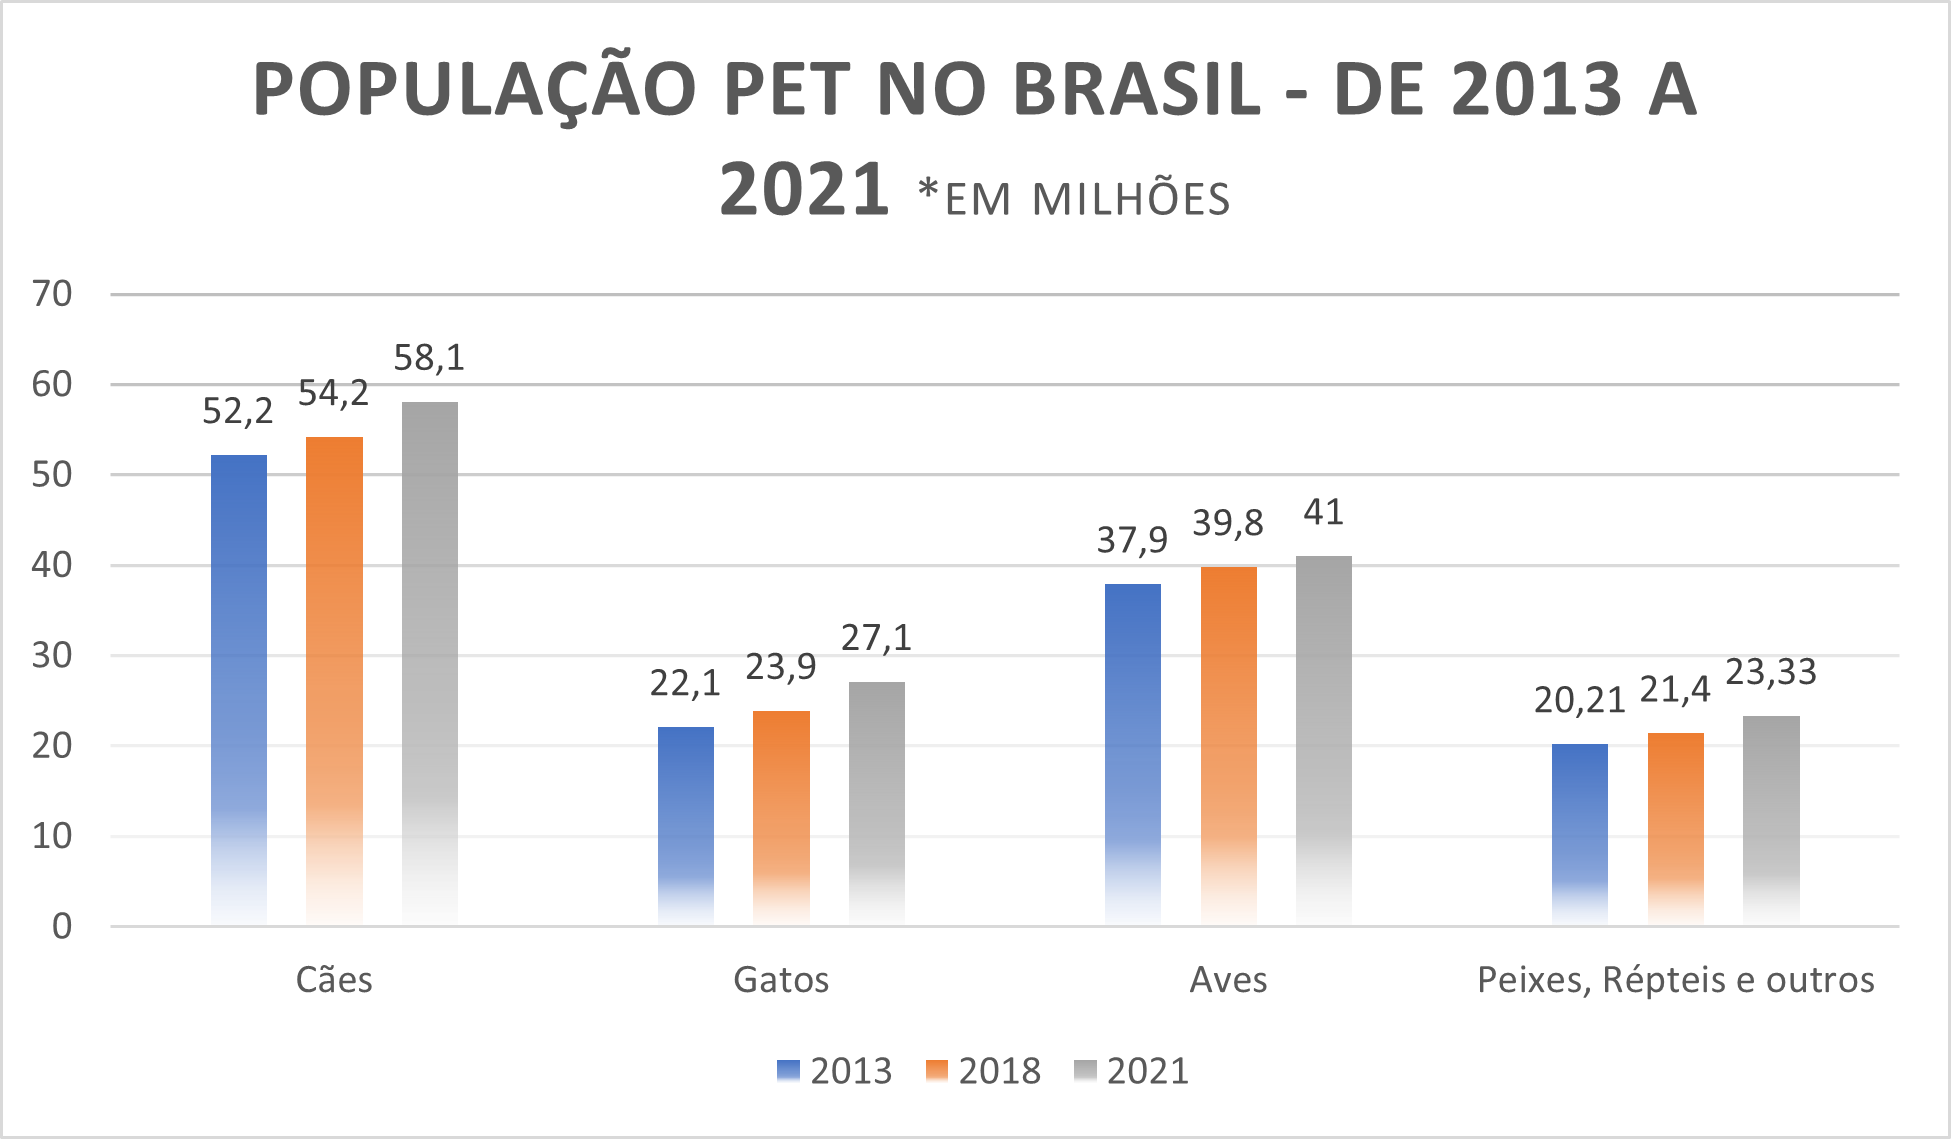
\includegraphics{images/grafico_censopet.png}
        \caption{Censo população Pet no Brasil, \citeonline{ibge2013, ibge2018, pet2021}}
        \label{fig:grafico_pet}
    \end{figure}

    \section{Análise da situação atual} \label{analise_atual}

    O documento obrigatório de maior valor durante o atendimento realizado pelo médico veterinário é, sem dúvidas, o prontuário veterinário. Atualmente são utilizados tanto versões físicas quanto versões digitais, ou eletrônicas, dos prontuários.

    Os prontuários eletrônicos são oferecidos por diversos sistemas de gerenciamento de clínicas veterinárias, por oferecerem armazenamento com acesso fácil aos dados dos prontuários, tendo em vista a declaração de João Abel Buck, médico-veterinário presidente da Associação Brasileira de Hospitais Veterinários (ABHV), fundada em 2017, por um grupo de empresários do segmento, em conversa com o CRMV-SP, onde garante que a transformação digital se apresenta de forma rápida, impulsionada pela pandemia que teve uma função catalisadora nisso, gerando uma grande necessidade do mercado de serviços veterinários em normatizar e regulamentar melhor este novo meio de se relacionar com os clientes utilizando da tecnologia como aliada \cite{buck}. Apesar da fidelidade das versões virtuais, os dados armazenados não podem substituir documentos físicos em eventos judiciais por não serem devidamente disciplinados por órgão regulamentador, nesse caso, pelos órgãos de classe que atestem a validade, \citeonline{pe_dig}, \citeonline{prontuario}.

    Além da questão regulatória, os sistemas de prontuários digitais atualmente disponíveis no mercado não torna os documentos imutáveis ou registram histórico de modificações. Assim, ao permitirem a alteração dos dados inseridos, sem permitirem consultar o histórico de alterações ou meios de rastreá-las, sujeita o estabelecimento ao risco de desamparo em caso de fiscalização por órgãos públicos ou perícias judiciais.

    Tendo em vista a dificuldade dos sistemas atuais de dar apoio em caso de fiscalizações e a premissa da existência de arquivos físicos, torna-se necessário manter os registros físicos em pastas-fichários após serem carimbados e assinados pelo médico veterinário, \citeonline{pe_dig}.

    O gerenciamento dos medicamentos controlados é realizado através de anotações manuais em um livro de registro. Esses registros devem ser realizados periodicamente e com exatidão pelo profissional veterinário, orientando e definindo os procedimentos a serem adotados dentro da clínica, a fim de prevenir descumprimentos das orientações. No entanto, demandam reserva de tempo e atenção para a execução de alguns desses procedimentos, como a operação de cálculos manuais para cada valor ou a repetição de anotações de mesmos dados em diferentes documentos, podendo interferir na performance e exigindo mais esforço do profissional, \citeonline{normativa}.

    Além das pontos fracos supracitadas, o armazenamento desses arquivos ocupa espaço físico e estão sujeitos a danos e perdas por mau armazenamento, como incidentes gerados por umidade, fogo, roubos e etc. O preenchimento desses dados em versões físicas e depois transcritos para versões digitais, pode ser um processo demorado e é sujeito a falhas, demandando um tempo que poderia ser melhor aplicado pelos profissionais envolvidos. Além disso, torna-se necessário um grau elevado de organização por parte da clínica, de tal modo que não prejudique que a consulta aos arquivos seja possível de forma a facilitar o serviço do profissional, \citeonline{pe_dig}.

    \section{Objetivos} \label{objetivos}

    A área de medicina veterinária ainda hoje opera de forma conservadora devido às suas necessidades burocráticas. E, por mais que o mercado ofereça algumas aplicações que têm a finalidade de automatizar o serviço, é difícil encontrar uma opção que ofereça funcionalidades que cumpram completamente as necessidades dos profissionais. Um dos motivos é que as soluções não são focadas em procedimentos específicos da veterinária, dividindo a ferramenta da aplicação com a gestão de Pet Shop.

    A aplicação, chamada de CertVet, tem como objetivo cobrir as principais necessidades de atuação do médico veterinário, automatizando os processos operacionais de atendimento e documentações clínicas, que hoje ainda demandam esforços manuais, garantindo o cumprimento de normas legais e regulamentares e propôr um fluxo do trabalho eficiente, diminuindo o tempo gasto neste, tendo em vista a observação da médica-veterinária, Mitika Kuribayashi Hagiwara, conselheira efetiva do CRMV-SP, professora sênior do Departamento de Clínica Médica e pesquisadora responsável pelo Grupo de Pesquisa em Patologia Clínica Veterinária, ambas da Faculdade de Medicina Veterinária e Zootecnia, da Universidade de São Paulo - FMVZ-USP, ao garantir em entrevista ao CRMV-SP que a necessidade de inserir informações dos animais atendidos por veterinários nos prontuários e em fichas clínicas de forma manual, demandava considerável espaço físico e muito mais tempo para busca e atualização dos dados, principalmente, em hospitais ou clínicas, onde há uma excessiva carga de serviços \cite{mitika}, sendo parte do escopo da CertVet, mitigar as problemáticas apontadas pela profissional, a fim de melhorar o desempenho do médico-veterinário, do atendimento e, consequentemente, da clínica.


    \section{Justificativa}\label{justificativa}

    Assim como o número de animais de companhia cresce a cada ano, a quantidade de profissionais veterinários atuantes no mercado brasileiro também apresenta crescimento, com 164.549 médicos veterinários inscritos de acordo com a contabilização do órgão federal, indicado na Figura \ref{fig:grafico vet}, \citeonline{vets_SP, vets2020, vets2022}.

    \begin{figure}[H]
        \centering
        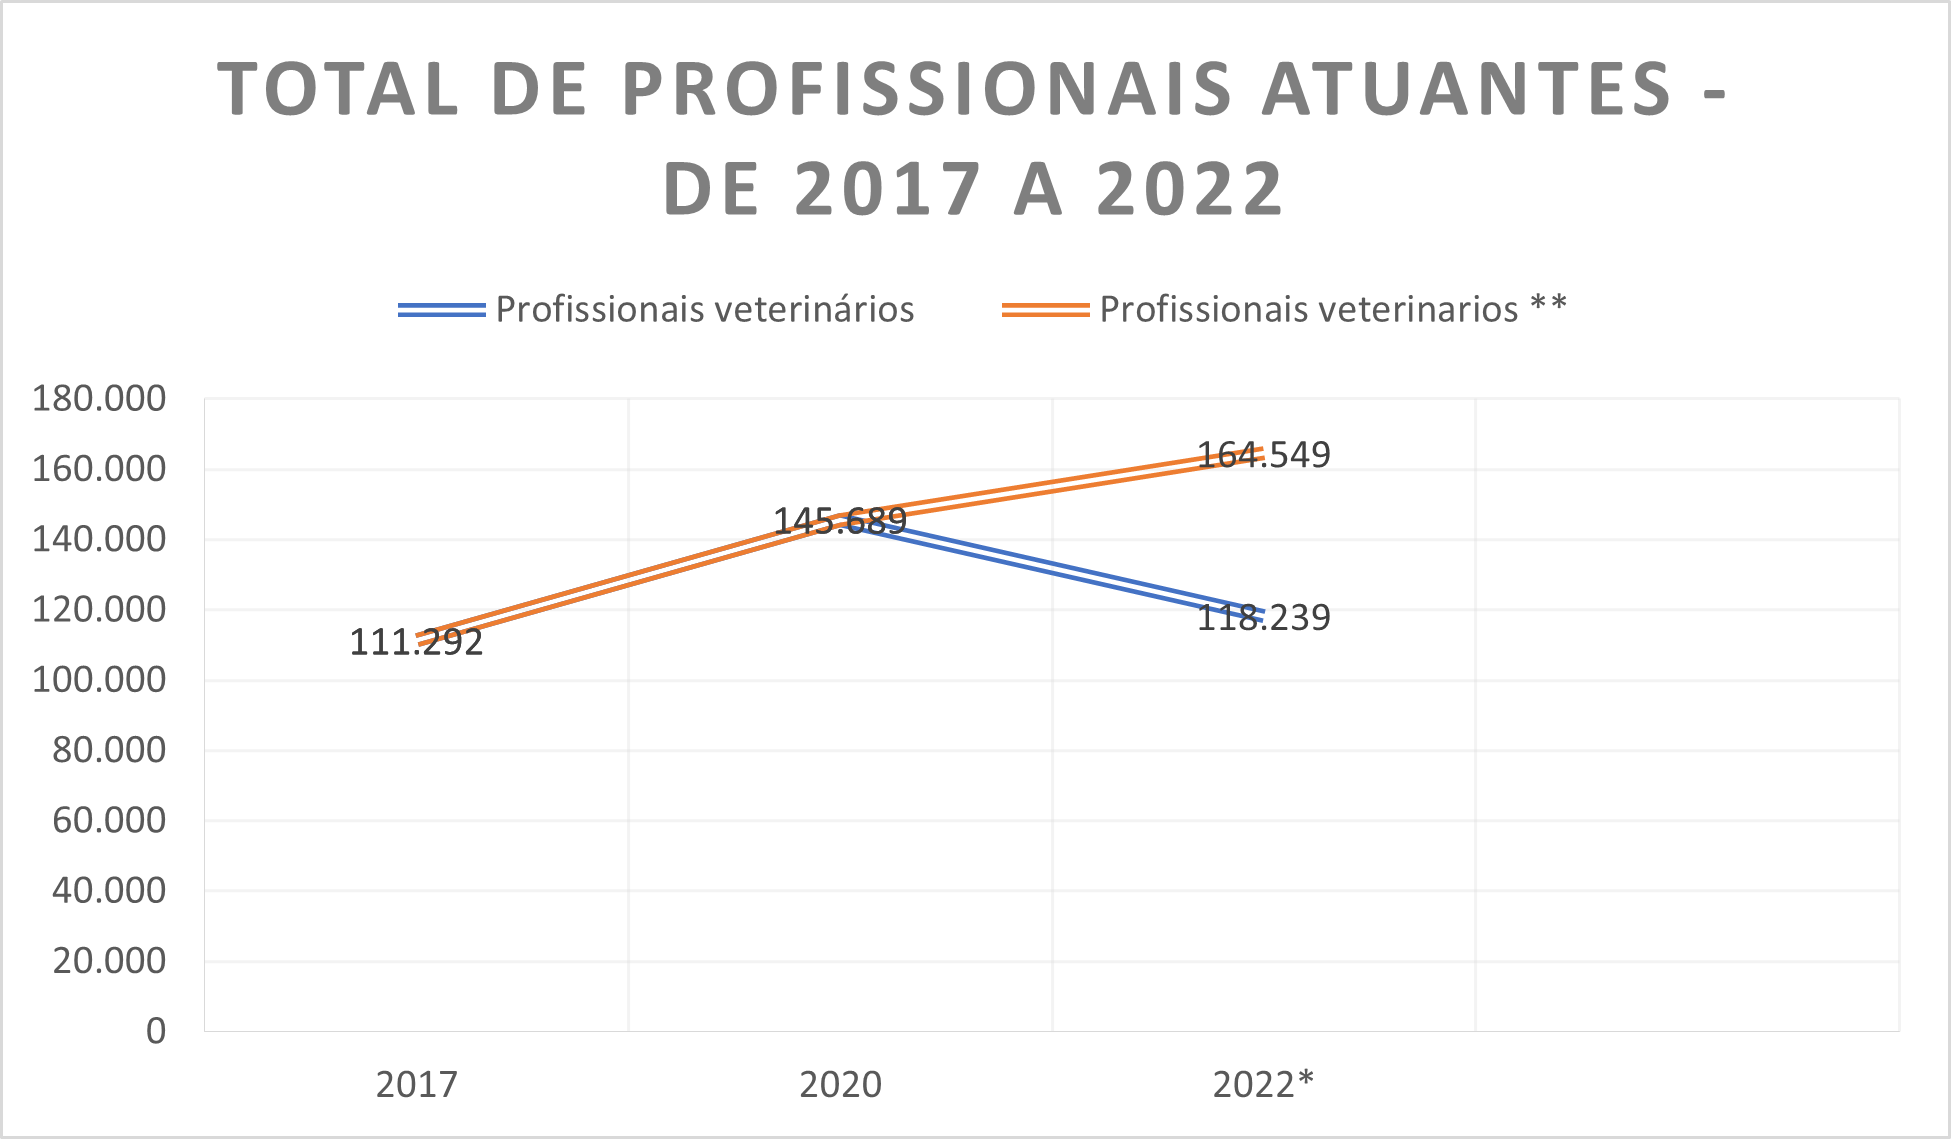
\includegraphics{images/grafico_profissionais.png}
        \caption{Número de veterinários registrados. *Dados sem os inscritos no Estado de São Paulo. ** Dados incluindo os inscritos no Estado de São Paulo.}
        \footnotesize {Fonte: \citeonline{vets2020,vets2022} }
        \label{fig:grafico vet}
    \end{figure}

    De acordo com o censo divulgado pelo CFMV para o biênio 2021/2022, atualmente existem 46.947 registros ativos de estabelecimentos veterinários, sendo divididos entre clínicas, hospitais, consultórios e ambulatórios, como podemos ver na Figura \ref{fig:grafico clinicas} \citeonline{clinicas2022}

    \begin{figure}[H]
        \centering
        \caption{Censo estabelecimentos veterinários no biênio 2021/2022}
        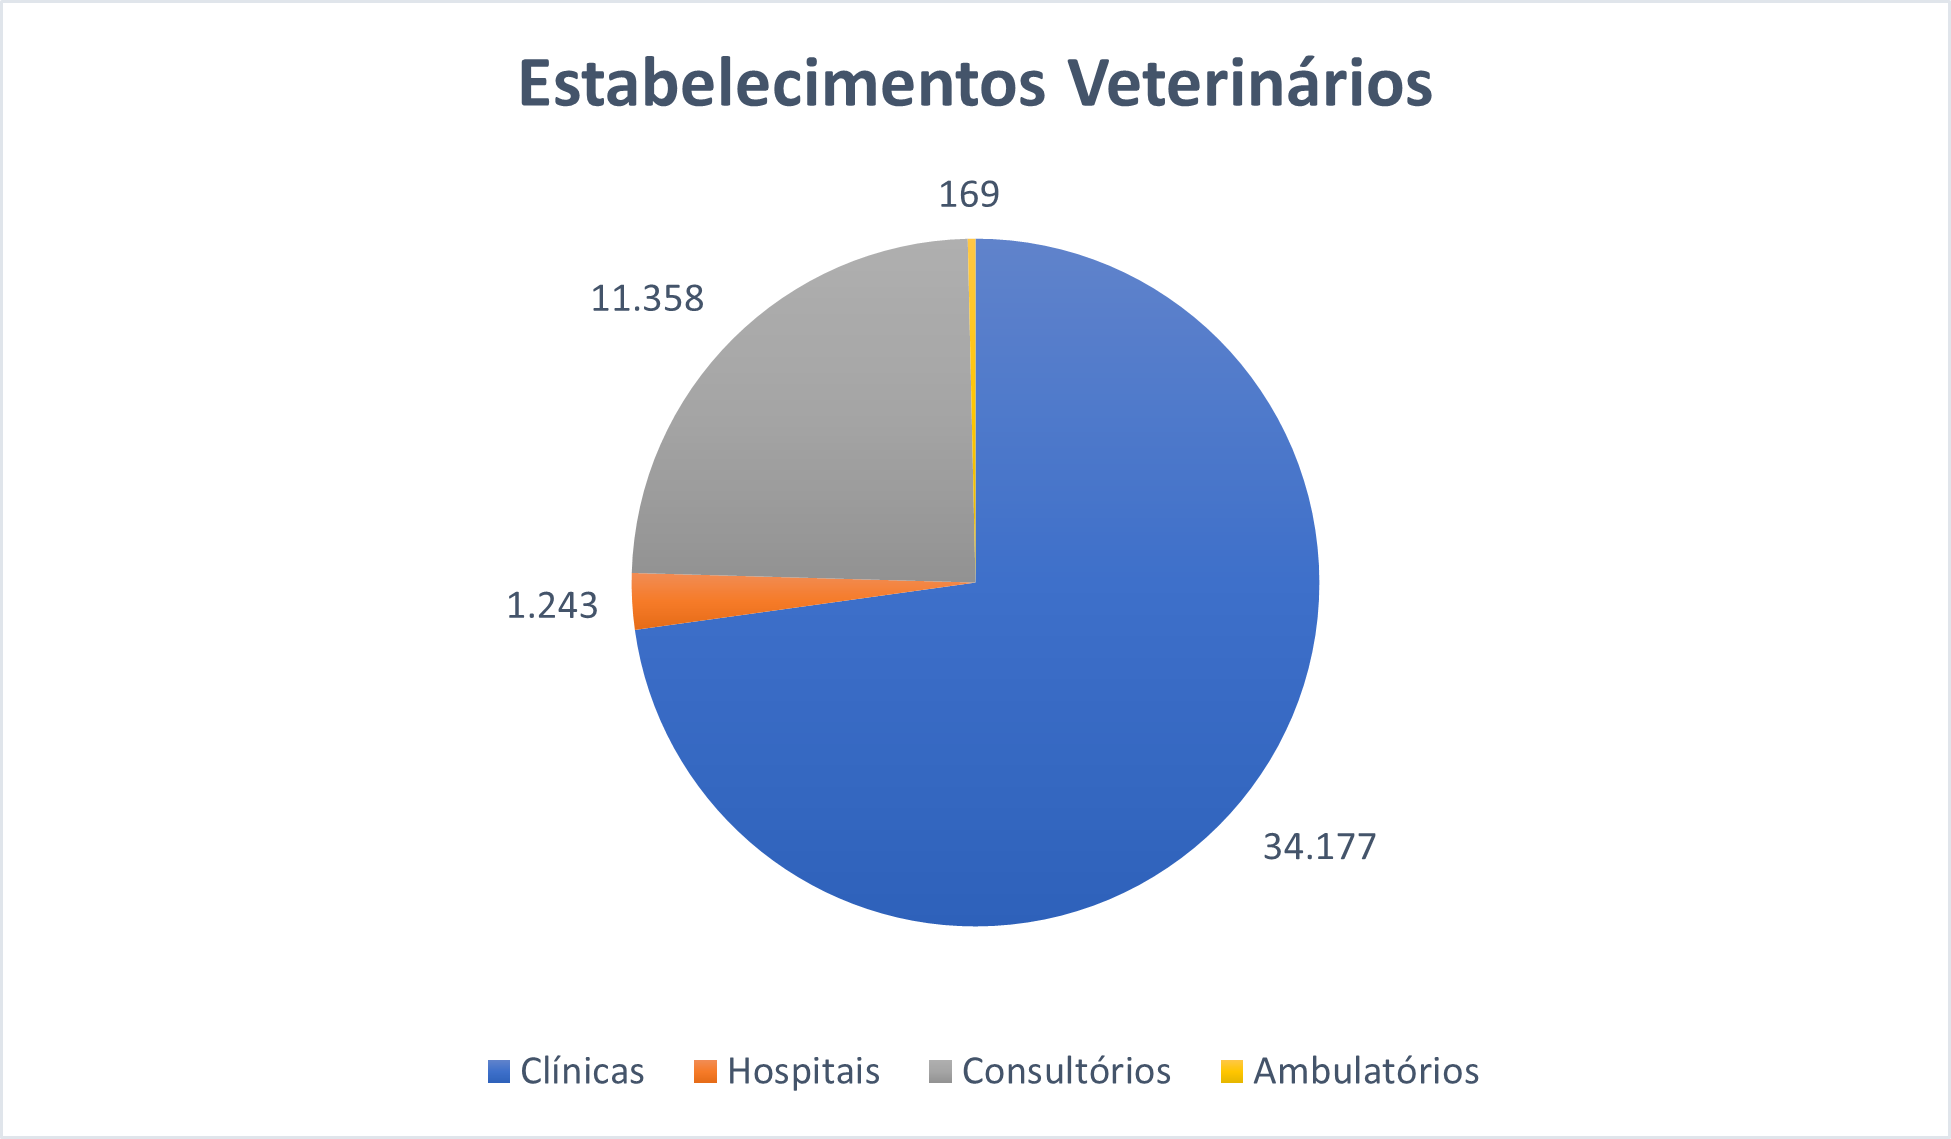
\includegraphics{images/grafico_estabelecimento.png}
        \footnotesize{ Fonte: \citeonline{clinicas2022}}
        \label{fig:grafico clinicas}
    \end{figure}

    Todos esses profissionais e estabelecimentos são fiscalizados e disciplinados pelas regras de conduta dos sistemas CFMV/CRMVs.

    Visando oferecer funcionalidades que permitam uma dinamização de todo o fluxo de trabalho do profissional veterinário, reduzir o tempo gasto com operações manuais, evitar a necessidades de anotações de informações repetidamente e reduzir o risco de erros de transcrição nas documentações, a CertVet consiste em um sistema que gerencia documentos com potencial valor legal e seus processos que se fazem necessários no fluxo de trabalho da medicina veterinária.

    Os processos automatizados agilizam os procedimentos fiscalizatórios e permitem que as alterações feitas sejam rastreadas, como é exigida pelo CFMV e pelos CRMVs \citeonline{teleMV}.

    A tecnologia da informação está modernizando a rotina de trabalho em áreas como automações de escritório, farmacêuticas e na medicina humana em estágios bem mais avançados que em relação ao atualmente aplicado na medicina veterinária. Compreende-se que existe a oportunidade de propor ritmo mais acelerado, garantindo a legalidade dos processos dentro de uma clínica veterinária.

    A partir das verificações de ambiente, referencial regulatório e constatação da situação, verificamos a necessidade do desenvolvimento de uma aplicação focada na automação de processos operacionais que otimizando o tempo de execução das tarefas do profissional veterinário e confiabilidade dos registros inseridos.

    Em pesquisa bibliográfica, não foram identificados fatos referentes à quantidade de profissionais ou estabelecimentos que utilizam algum sistema eletrônico ou de gestão. Porém, os meios de comunicação comumente enfatizam o crescimento de relevância econômica de serviços para o mercado de animais de estimação ano a ano. O sistema CertVet tem potencial para crescer e se destacar entre os demais sistemas já existentes.

    \section{Análise de Concorrência} \label{analise_concorrência}

        Nos últimos anos ocorreu modernização na dinâmica que rege a profissão do médico veterinário tanto pelo CFMV, como por seus órgãos regionais \citeonline{art_digital} \citeonline{cart_digital}, possibilitando que documentos obrigatoriamente físicos pudessem ser registrados em versões digitais válidos em todo território nacional. 

        A solicitação de tais documentos também pode ser realizada via navegação humana por sistema \emph{web} disponibilizado publicamente pelo CFMV, utilizando meios de identificação e autenticação nos sistemas regentes \citeonline{art_digital}. Este mesmo dado também pode ser utilizado por interface de aplicação, uma vez liberado por usuário habilitado por intermédio do CFMV.

        Para fins de comparação, foram selecionadas seis aplicações, já populares no mercado, que atuam na mesma problemática da CertVet.

    \subsection{SimplesVet}
    O SimplesVet se apresenta como um sistema para petshop e clínica veterinária que busca ajudar a simplificar a rotina da clínica \citeonline{simplesvet}. Consiste em um sistema acessado via \emph{web}, permitindo o controle da clínica a qualquer hora ou lugar, contanto que tenha acesso a internet. Suas funcionalidades dividem-se em:

\begin{itemize}

    \item Atendimento veterinário: permite o registro das fichas veterinárias em uma tela simples, com dados salvos na nuvem.
    \item Agenda de serviços: possibilita a organização da agenda dos veterinários e envia lembretes sobre os próximos atendimentos.
    \item Internação veterinária: organização dos prontuários e agendas de plantão.
    \item Controle financeiro: possibilita a organização do fluxo de caixa da clínica e envia lembretes de contas a pagar no celular cadastrado.
    \item Gestão de estoque: visualização dos produtos a repor, itens próximos ao vencimento, produtos parados e etc.
    \item Análise de vendas: visualização de um dashboard voltado à estratégias de \emph{marketing}, listando produtos mais vendidos, ticket médio, horários de pico e etc.
    \item Notas fiscais: emissão de nota fiscal de consumidor eletrônica (NFC-e), nota fiscal de serviços eletrônica (NFS-e) e nota fiscal eletrônica (NF-e).
    \item \emph{App} para tutores: um \emph{app} feito para o cliente com datas de vacinação, exames e informações do pet.
    \item Mensagens automáticas: envio de lembrete de consultas e vacinas para os tutores e agenda para veterinários.
    \item \emph{Short Message Service (SMS) Marketing}: envio de campanhas via mensagens de texto para os clientes.
    \item Pesquisa e satisfação: possibilita o recebimento de avaliações dos clientes para fins comparativos com o mercado.
\end{itemize}

A SimplesVet possui mais \emph{features} voltadas à gerência de assuntos de \emph{PetShop}, como controle de estoque e de vendas, cumprindo de forma básica apenas uma das demandas da clínica veterinária \citeonline{simplesvet}. Enquanto a Certvet tem como principal objetivo resolver de forma simples as demandas do ambiente clínico, voltadas principalmente ao trabalho realizado pelo veterinário, como: manutenção de prontuário digital, controle de internação, controle da medicação e da autenticação de receitas, dentre outras, resolvendo demandas que não são contempladas pelo SimplesVet.

        \subsection{Vetwork}
        O Vetwork destaca-se entre os usuários pela sua interface intuitiva sendo algo que auxilia na produtividade do trabalho, trata-se de um sistema de gestão baseado na nuvem, não sendo necessária a instalação de hardware ou software, pois funciona nativo como \emph{Software as a Service (SaaS)} \citeonline{vetwork}. Seus 2.744 usuários dispõem das seguintes funcionalidades:

\begin{itemize}
    \item Agenda vinculada ao caixa: um controle geral das atividades realizadas nos \emph{pets}, como consultas médicas, retornos, exames, cirurgias, banhos, tosas e todos os outros procedimentos, sem limite de datas.
    \item Gestão de Documentos: permite a inclusão de documentos e arquivos à ficha clínica do animal, como laudos, fotografias, exames de imagem e outros, que são armazenados na internet e podem ser acessados de qualquer lugar.
    \item Calendário: uma forma de controle das datas e horários em que os animais passaram por procedimentos como banhos, tosas, exames, consultas, vacinas ou quaisquer outros realizados no estabelecimento.
    \item Gestão clínica: criação de prontuário eletrônico com as informações médicas do pet, como controle de registros clínicos, exames, vacinas e doses adicionais.
    \item Gestão Financeira: controle de caixa, pacotes, contas a pagar e a receber, pagamentos pendentes e pré-vendas, cálculo de comissionamento e geração de relatórios financeiros da empresa.
    \item Relacionamento com o Cliente: armazenamento de todas as informações dos clientes para possibilitar um relacionamento mais próximo com o mesmo.
    \item \emph{E-mail} Inclusos: mensagens automáticas, através de \emph{e-mail}, para comunicação instantânea.
\end{itemize}

    Apesar de ser uma aplicação mais completa em relação à anterior, ainda assim o prontuário eletrônico é o ponto forte desse serviço, no que tange à funcionalidades para o fluxo clínico veterinário \citeonline{vetwork}. A CertVet busca resolver de forma eficaz e mais completa, o controle de medicamentos, não só o seu cadastro e quantidade em estoque, mas o uso de uma chave de autenticação para receitas e a aplicação dos mesmos. De forma resumida, o Vetwork é sim uma ferramenta bem útil mas a aplicação aqui proposta resolve demandas que não são resolvidas por esse serviço, por mais que suas avaliações no mercado sejam positivas.

        \subsection{DoctorVet}
        O DoctorVet é um sistema totalmente voltado à gestão de clínicas e hospitais veterinários e apresenta duas versões: uma \emph{Standard} com módulos para controle de consultas, vacinas, pequenas cirurgias, assuntos de pet shop e também financeiro. E uma versão enterprise que contempla todos os módulos \emph{Standard} e adicionalmente um controle de internação e hospedagem e concentra informações do centro cirúrgico e laboratório \citeonline{doctorvet}.  Funcionalidades da versão \emph{Enterprise} do DoctorVet:

\begin{itemize}
    \item Módulo de Cadastro: realiza o cadastro de veterinários, funcionários, animais, clientes e planos de atendimento.
    \item Módulo Farmacológico: permite o cadastro de vacinas, vermífugos e o cadastro de procedimentos ou interações medicamentosas.
    \item Módulo Atendimento: criação de ficha de atendimento, lista de espera, curadoria de orçamentos, central de   agendamentos e controle de status do veterinário.
    \item Módulo Caixa: utilizado pelos atendentes de caixa, controle das formas de recebimento, abertura e fechamento do caixa e manutenção.
    \item Módulo Consultório: consultas generalistas e especialistas, histórico de consultas e atendimentos, pedidos de exames, receituários e prontuário eletrônico.
    \item Módulo Pet Shop: permite televendas, consulta de preços e relatórios e emissão de cupom fiscal.
    \item Módulo Internação Básica/Avançada: admissão de internação, controle da evolução do quadro clínico, alta veterinária, manter prontuários, cadastro de prescrições.
    \item Módulo Estoque: cadastro de fornecedores, cadastro e etiquetação de produtos, gerenciamento de lotes, requisições à farmácia e requisições internas, controle de compras e relatórios.
    \item Módulo Exames: controle de exames laboratoriais e seus resultados.
    \item Módulo Laboratório: cadastros, central de coleta e composição de exames.
    \item Módulo Centro Diagnóstico: preparo para exames e suas composições.
    \item Módulo Relatórios: criação de relatórios operacionais, gerenciais e estratégicos em concordância com Gestão de Relacionamento com o Cliente (CRM), Sistema Público de Escrituração Digital Fiscal (SPED), Programa de Integração Social (PIS) e Contribuição para o Financiamento da Seguridade Social (Cofins).
    \item Módulo Segurança: cadastro de usuários e permissões de acesso de acordo com níveis.
\end{itemize}

    É a aplicação mais recente das selecionadas e também a mais completa, no entanto, reforça-se aqui que não contempla o controle de medicamentos \citeonline{doctorvet}, oferecido pela Certvet.

        \subsection{Dr. Snoopy Smart}
        O Dr. Snoopy Smart se apresenta como um sistema completo de gestão exclusivo para Pet Shop e clínicas veterinárias, automatizando processos clínicos, na tentativa de agilizar as tarefas e tendo o aumento das vendas como foco do módulo de pet shop \citeonline{drsnoopy}. Consiste em um software com as seguintes funcionalidades:

\begin{itemize}
    \item Agendamento otimizado: permitindo o controle de agendamento dos pacientes.
    \item Gerenciamento de estoque: visibilidade da quantidade de produtos e quais estão em falta.
    \item Prontuário Clínico: possibilita a criação e consulta da ficha veterinária dos animais.
    \item Emissão de Notas: emissão de nota fiscal eletrônica (NF-e), nota fiscal de serviços eletrônica (NFS-e) e cupons fiscais.
    \item Histórico de Pacientes: arquivação e consulta de informações dos atendimentos. 
    \item Vacinas sempre em dia: controle de quando o paciente deve ser vacinado.
    \item Agenda de Banho e Tosa: específica para tais, permitindo um maior controle do pet shop.
    \item Gestão Integrada: permite acessar à determinados indicadores de gestão.
    \item Notificações \emph{Short Message Service} (SMS): recebimento de lembretes importantes no celular dos usuários da aplicação
    \item Relatórios Personalizados: geração de relatórios com facilidade.
\end{itemize}

    Apesar de ser uma aplicação com muitas funcionalidades, ainda assim não apresenta as opções de modernidade que a aplicação aqui proposta oferece, considerando-se que divide o escopo clínico com as necessidades de um pet shop, apresentando mais funcionalidades voltadas à gestão e estratégias de venda do que para o fluxo de trabalho do profissional veterinário.

        \subsection{Vetsoft}
        O programa VetSoft é oferecido nas versões \emph{Desktop} e \emph{Web}, sendo essa primeira uma versão instalada nos computadores em rede, permitindo o acesso mesmo com falta de conexão com a \emph{internet}. E a versão \emph{Web}, um sistema em nuvem que permite ao usuário gerenciar o negócio através de diferentes dispositivos, seja pelo computador ou pelo \emph{smartphone}, contanto que tenha acesso à internet \citeonline{vetsoft}. O VetSoft abrange serviços de clínica veterinária, hospital veterinário, \emph{pet shop} / banho e tosa e veterinários autônomos com as seguintes funcionalidades:

\begin{itemize}
    \item Ficha do Tutor: ficha cadastral da conta do tutor e seus animais, visibilidade do histórico de pagamentos e envio de e-mail individual.
    \item Ficha do Animal: ficha cadastral específica dos animais pacientes, álbum de fotos, agendamentos, agrupamento dos resultados de exames e histórico de vacinas e vermífugos.
    \item Histórico Clínico: anamnese, diagnóstico, laudo clínico, receituário normal e especial e exames.
    \item Gestão de Estoque: divisão de produtos por grupos, controle de produtos com estoque baixo, visibilidade dos produtos mais e menos vendidos e entrada de estoque manual e XML.
    \item Financeiro: controle de caixa diário e seu fluxo, demonstrativo de resultados por área, centro de custos, controle de planos para clientes mensalistas.
    \item Emissão Fiscal: possibilidade de emissão fiscal para todos os estados e os formatos: Nota Fiscal de Consumidor Eletrônica (NFCe), Sistema Autenticador e Transmissor de Cupons Fiscais Eletrônicos (SAT), Módulo Fiscal Eletrônico (MFe) e Programa Aplicativo Fiscal – Emissor de Cupom Fiscal (PAF-ECF).
    \item Farmácia/Materiais: controle de estoque de farmácia e materiais de uso interno.
    \item Imunizações: controle da aplicação de vacinas e vermífugos na ficha do animal com agendamentos e aplicações realizadas.
\end{itemize}

    É uma das aplicações mais completas, no entanto, o controle de medicamentos oferecido não atinge o mesmo grau de segurança que a chave de autenticação para as receitas que a CertVet oferece, assumindo um papel importante na modernização dessa autenticação nos dias atuais.

        \subsection{BensVet}
        O BensVet se diferencia dos demais apresentados por se tratar de um serviço que se divide em dois aplicativos, um para uso veterinário e um para uso dos tutores. O aplicativo para veterinários garante que o usuário poderá iniciar um atendimento a domicílio e conseguir  dar continuidade na clínica. E o aplicativo para tutores trata-se dos processos de envio  de promoções e alertas de retorno automáticos para os tutores, permitindo também a consulta de  informações sobre o animal e agendamento de atendimentos pelo \emph{App},  \citeonline{bensvet}. As funcionalidades dividem-se em:

\begin{itemize}
    \item Agenda de atendimentos.
    \item Acompanhamento de medicações na internação.
    \item Criação de fichas clínicas personalizadas.
    \item Notificar automaticamente consultas, retornos e vacinas aos clientes.
    \item Consultar históricos de animais e seus tutores.
    \item Controle dos comissionamentos de profissionais.
    \item Emitir Notas Fiscais referente a venda de produtos.
    \item Controle de estoque.
\end{itemize}

    Trata-se de uma resolução que se aproxima bastante da CertVet no que tange à proximidade do profissional veterinário, esteja ele numa clínica ou trabalhando de forma autônoma, no entanto, observamos aqui que o controle de medicamentos oferecido, mais uma vez, não atinge o mesmo grau de segurança que a chave de autenticação aqui propostas, além da funcionalidade de consulta ao histórico de aspectos hereditários.

    \subsection{Quadro comparativo de concorrentes}
    Com base no levantamento acima, foi possível observar algumas intersecções das funcionalidades oferecidas. O Quadro \ref{tab:comparativa} permite melhor visualização deste levantamento.

    \begin{center}
    \begin{quadro}[H]
     \caption{Comparação das aplicações concorrentes}
    \label{tab:comparativa}
    \begin{tabulary}{1.0\textwidth}{|L|L|L|L|L|L|L|L|L|}
    \hline
     & CertVet & Simples Vet & Vet work & Doctor Vet & Dr. Snoopy Smart & Vet soft & Beans Vet\\
    \hline
    Agenda & x & x & x & x & x & x & x\\
    \hline
    Prontuário clínico & x & x & x & x & x & x & x\\
    \hline
    Gerenciamento de medicação & x & x &  & x & x & x & x\\
    \hline
    Controle de vacina\c{c}ão & x &  &  & x & x & x & x\\
    \hline
    Histórico de Aspectos Hereditários & x &  &  &  &  &  & \\
    \hline
    Rastreio de alterações & x &  &  &  &  &  & \\
    \hline
    Gestão Financeira &  & x & x & x & x & x & x\\
    \hline
    Gestão PetShop &  & x & x & x & x & x & x\\
    \hline
    \end{tabulary}
    \centering
    {\footnotesize Fonte: Elaborado pelos autores.}
    \end{quadro}
\end{center}

\chapter[Revisão de Literatura]{Revisão da Literatura} \label{revisao_lit}

    Este capítulo aborda uma breve revisão bibliográfica sobre a documentação obrigatória emitida por estabelecimentos veterinários, revisão das leis referentes a tais documentos, novos caminhos abordados pelo Conselho Federal de Medicina Veterinária e como esse aspectos são relevantes ao nosso projeto.


    \section{Documentação Obrigatória e Legislação Pertinente}

        De acordo com a Resolução nº1321, de 24 de abril de 2020 \citeonline{doc_obrig}, todo estabelecimento veterinário e/ou médico veterinário deve emitir documentos específicos no âmbito de suas respectivas atividades profissionais.

        Tais documentos, de caráter obrigatório, deve seguir os padrões estabelecidos pelo Conselho Federal de Medicina Veterinária, que regulamenta a profissão do médico veterinário, de acordo com a Lei nº 5.517, alínea “f”, do artigo 16, de 23 de outubro de 1968. \citeonline{doc_obrig}.

        A Resolução 1321/2020, em seu Art. 2º, define o prontuário veterinário como \citeonline{doc_obrig}: 

        \begin{citacao}

        
            VIII - prontuário médico-veterinário: documento escrito e datado, sem rasuras ou emendas, emitido e assinado, privativamente por médico-veterinário que relata e detalha, cronologicamente, informações e dados acerca dos atendimentos ambulatoriais e clínicos, inclusive vacinações, exames diagnósticos e intervenções cirúrgicas realizados em animal, ou coletivo em se tratando de rebanho, garantida a autenticidade e integridade das informações;
        \end{citacao}

        Outros documentos obrigatórios estão dispostos no Quadros \ref{doc_obrigatorio_demanda}, \ref{doc_obrigatorio_demanda2} e \ref{quad:documentos3}: 

\begin{center}
    \begin{quadro}[H]
    \caption{Relação de Documentos de Caratér Obrigatórios e Demanda}
    \label{doc_obrigatorio_demanda}
    \begin{tabulary}{1.0\textwidth}{|p{10em}|p{15em}|p{10em}|}
    \hline
    Nome & Objetivo do documento & Obrigatoriedade\\
    \hline
    Atestado ou declaração de óbito (Anexo \ref{atestado de obito}) & Documento escrito e datado, sem rasuras ou emendas, emitido e assinado, privativamente, por um médico-veterinário para declarar o óbito do animal e a provável causa mortis & Não, disponível sob demanda\\
    \hline
    Atestado ou declaração de vacinação (Anexo \ref{atestado de vacina}) & Documento escrito e datado emitido e assinado, privativamente, por um médico-veterinário para declarar o ato vacinal com a devida identificação do animal vacinado & Sim, quando houver necessidade de ato vacinal\\
    \hline
    Atestado sanitário (Anexo \ref{atestado sanitario}) & Documento escrito, sem rasuras ou emendas, datado, emitido e assinado privativamente por um médico-veterinário para declarar o estado ou condições de saúde do(s) animal(is) & Não, disponível sob demanda\\
    \hline
    Prontuário médico-veterinário (Anexo \ref{atestado de obito}) & Documento escrito e datado, sem rasuras ou emendas, emitido e assinado, privativamente por um médico-veterinário que relata e detalha, cronologicamente, informações e dados sobre os atendimentos ambulatoriais e clínicos, inclusive vacinações, exames diagnósticos e intervenções cirúrgicas realizados em animal, ou coletivo em se tratando de rebanho & Sim, em todo atendimento clínico veterinário\\
    \hline
    Termo de consentimento livre esclarecido para realização de exames (Anexo \ref{consentimento exame}) & Documento a ser apresentado por médico-veterinário para assinatura do responsável pelo animal com o objetivo de formalizar a ciência e livre consentimento ou autorização para realização de exames veterinários & Sim, quando houver necessidade de realizar exame(s)\\
    \hline
    Termo de consentimento livre esclarecido para realização de procedimentos terapêuticos de risco ou experimental (Anexo \ref{consentimento tratamento}) & Documento a ser apresentado por médico-veterinário para assinatura do responsável pelo animal com o objetivo de formalizar a ciência e livre consentimento ou autorização para realização de procedimento terapêutico que tenha elevado grau de comprometimento ou perda de sentido ou função, debilidade ou deformidade, bem como óbito & Sim, quando houver necessidade de realizar procedimento(s) terapêutico(s)\\
    \hline
    \end{tabulary}
    \centering
    \footnotesize {Fonte: \citeonline{doc_obrig}}
    \end{quadro}
\end{center}

\begin{center}
    \begin{quadro}[H]
    \caption{Relação de Documentos de Caratér Obrigatórios e Demanda - continuação }
    \begin{tabulary}{1.0\textwidth}{|p{10em}|p{15em}|p{10em}|}
    \hline
    Nome & Objetivo do documento & Obrigatoriedade\\
    \hline    
    Termo de consentimento livre esclarecido para retirada de corpo de animal em óbito (Anexo \ref{retirar corpo}) & Documento a ser apresentado por médico-veterinário para assinatura do responsável pelo animal com o objetivo de esclarecer e transferir a esse a responsabilidade pela posse e destinação ambiental adequada do cadáver & Não, disponível sob demanda\\
    \hline
    Termo de consentimento livre esclarecido para realização de procedimento cirúrgico (Anexo \ref{consentimento cirurgico}) & Documento a ser apresentado por médico-veterinário para assinatura do responsável pelo animal com o objetivo de formalizar a ciência e livre consentimento ou autorização para realização de procedimento cirúrgico & Sim, quando houver necessidade de realizar procedimento(s) cirúrgico(s)\\
    \hline
    Termo de consentimento livre esclarecido para realização de procedimento anestésico (Anexo \ref{consentimento anestesico}) & Documento a ser apresentado por médico-veterinário para assinatura do responsável pelo animal com o objetivo de formalizar a ciência e livre consentimento ou autorização para realização de procedimentos de anestesia & Sim, quando houver necessidade de realizar procedimento(s) cirúrgico(s)\\
    \hline
    Termo de consentimento livre esclarecido para internação e tratamento clínico ou pós-cirúrgico (Anexo \ref{consentimento internacao}) & Documento a ser apresentado por médico-veterinário para assinatura do responsável pelo animal com o objetivo de formalizar a ciência e livre consentimento ou autorização para realização de internação e tratamento clínico ou pós-cirúrgico & Sim, quando houver necessidade de internação e tratamento clínico ou pós-cirúrgico\\
    \hline
    Termo de consentimento livre esclarecido para realização de eutanásia (Anexo \ref{consentimento eutanasia}) & Documento a ser apresentado por médico-veterinário para assinatura do responsável pelo animal com o objetivo de formalizar a ciência e livre consentimento ou autorização para realização de eutanásia no animal & Não, disponível sob demanda\\
    \hline
    \end{tabulary}   
    \label{doc_obrigatorio_demanda2}
    \centering
    \footnotesize {Fonte: \citeonline{doc_obrig}}
    \end{quadro}
\end{center}


%%%%%%%%%%%%%%%%%%%%%%

\begin{center}

    \begin{quadro}[H]
    \caption{Relação de Documentos Obrigatórios e Demanda - continuação}
    \begin{tabulary}{1.0\textwidth}{|p{10em}|p{15em}|p{10em}|}
    \hline
    Nome & Objetivo do documento & Obrigatoriedade\\
    \hline
    Termo de consentimento livre esclarecido para retirada do serviço veterinário sem alta médica (Anexo \ref{retirada sem alta}) & Documento a ser apresentado por médico-veterinário para assinatura do responsável pelo animal com o objetivo de esclarecimento e obtenção da manifestação de livre intenção de retirada do animal de serviço veterinário sem alta médica, bem como de assunção de plena e irrestrita responsabilidade sobre os riscos sanitários e de morte do animal & Não, disponível sob demanda\\
    \hline   
    Termo de consentimento livre esclarecido para doação de corpo de animal para ensino e pesquisa (Anexo \ref{doacao de corpo}) & Documento a ser apresentado por médico-veterinário para assinatura do responsável pelo animal com o objetivo de esclarecimento e obtenção da manifestação de livre doação do corpo do animal para encaminhamento a instituição de ensino e pesquisa & Não, disponível sob demanda\\
    \hline
    Termo de consentimento livre esclarecido para realização de pesquisa clínica (Anexo \ref{atestado de obito}) & Documento a ser apresentado por médico-veterinário para assinatura do responsável pelo animal com o objetivo de esclarecimento e obtenção de autorização de submissão do animal a estudo ou pesquisa & Não, disponível sob demanda\\
    \hline
    \end{tabulary}   
    \label{quad:documentos3}
    \centering
    {\footnotesize Fonte: \citeonline{doc_obrig}}
    \end{quadro}
\end{center}

        Dentre as regras referidas na Resolução nº 1321 de 2020, seu artigo 3º disciplina dados para a composição do prontuário médico:

        \begin{citacao}

        
            Os documentos emitidos por médicos-veterinários comporão o prontuário do paciente (...) conter os seguintes dados e informações: nome completo e assinatura do médico-veterinário, número de inscrição no Sistema CFMV/CRMVs, endereço, telefone,\emph{e-mail} e, se for o caso, identificação do estabelecimento (razão social, CNPJ e número de registro no Sistema CFMV/CRMVs)
        \end{citacao}

            No inciso VI, especifica fatos relacionados ao animais que devem constar por observação física:

        \begin{citacao}

            (Deve) conter informações que permitam a identificação do paciente, tais como nome, sexo, raça, idade real ou presumida, cor de pelagem ou plumagem, sinais particulares, tatuagem, brinco, \emph{microchip}, registro genealógico e, conforme o caso, resenha detalhada;(...) identificação do responsável pelo animal (nome completo, CPF e endereço completo)
        \end{citacao}

        Em seu inciso VII, § 2º, dispõe sobre requisitos para operação de através de mídias virtuais: 

        \begin{citacao}
            Os documentos expedidos eletronicamente deverão contar com sistemas capazes de garantir a segurança, autenticidade, confidencialidade e integridade de informações, bem como o armazenamento e compartilhamento dos dados.
        \end{citacao}

           As regulamentações acima garantem a legitimidade do sistema proposto, pois servem de embasamento legal e diretrizes a serem seguidas.

        A autorização para se realizar a telemedicina na área veterinária também adere à tendência de modernização na profissão e viabiliza que soluções digitais sejam implementadas relativas a documentação obrigatória.\citeonline{teleMV}.

        Com relação à gestão de medicamentos controlados (de uso restrito e com retenção de receitas), de acordo com as leis vigentes da Instrução Normativa nº 35, de 11 de setembro de 2017, Capítulo I, Art. 2º, § IV, Capitulo IV, § 11  \citeonline{normativa}, ela é realizada através de um caderno de capa dura, no formato brochura, no qual o médico veterinário Responsável Técnico (RT) anota a data de entrada dos medicamentos no estoque e quanto desse medicamento foi utilizado no dia, para cada procedimento. Este caderno é denominado Livro-Registro.

    \section{Diferença entre Prontuário e Histórico Médico }

    De acordo com o Conselho Federal de Medicina (CFM), prontuário médico é um documento que apresenta todos os dados relativos ao paciente, como o histórico familiar, anamnese, descrição e evolução de sintomas e exames realizados por esse paciente, além de prescrições de tratamento a ser seguido. Esse documento tem como objetivo facilitar a assistência ao paciente. Embora feito durante o atendimento médico no consultório ou hospital, o paciente é considerado o proprietário desse registro podendo ter acesso e solicitar cópias, \citeonline{prontuario_medico}.


    Em contrapartida, o histórico médico é um documento cujo objetivo é registrar todas as informações relevantes do paciente sobre sua saúde, contribuindo dessa maneira para a análise completa do quadro de saúde do paciente por profissionais da saúde. Nesse documento deverão ser registrados não apenas o histórico de doenças, mas informações sobre consultas prévias que esse paciente teve durante a sua vida, \citeonline{historico_medico}, hábitos e doenças. Esse documento ajuda na prevenção de patologias, visto que esse sinaliza possíveis fatores de risco à saúde do paciente. %(https://telemedicinamorsch.com.br/blog/historico-do-paciente)

    A diferença entre histórico médico e prontuário, embora seja muito sutil, esta existe e consiste no fato de que o histórico médico apresenta um dados cronológicos sobre o paciente, ou seja, o que ele já teve e o que ele está tendo, enquanto o prontuário não faz relação com seu histórico, limitando-se a registrar as informações do paciente e de seu tratamento para uma determinada situação, \citeonline{prontuarioXhistorico}. 

\chapter[Metodologias]{Metodologias}

    O projeto propõe a criação de um sistema de gerenciamento de processos e documentação exigidas pelo órgão de classe veterinária, além de implementar funcionalidades já existentes em outros sistemas de gestão de estabelecimentos veterinários. 

    \section{Proposta}

        Tendo em vista os pontos fracos das soluções disponíveis atualmente, anteriormente mencionados no Capítulo \ref{objetivos}, a CertVet oferece a gestão das atividades do médico-veterinário, cobrindo o fornecimento de informações gerenciais de toda a clínica, como os cadastro de funcionários e clientes e as informações que se fazem necessárias. 

        No segmento de atendimento veterinário, a aplicação oferece o recurso de prontuário clínico digital, no qual permite a análise rápida de todo histórico assistencial dos animais, aplicando a assinatura eletrônica a esses arquivos, utilizando um certificado digital válido padrão ICP-Brasil, sendo esse o processo responsável por garantir a verificabilidade e rastreabilidade de alterações feitas, bem como os devidos registros de data e hora, sendo assim, passível de fiscalização.

        Complementarmente, para os registros de medicamentos controlados, é possível cruzar os dados movimentação de determinados medicamentos disponíveis no estoque, suas movimentações no livro-registro e valores desses medicamentos que estão sendo utilizados durante os procedimentos, atribuindo maior consistência aos registros e diminuindo o retrabalho de se adicionar as mesmas informações manualmente. O sistema realiza os cálculos de quantidade de medicamentos utilizados e atualiza-os no livro-registro digital.

    \section{Funcionalidades}

        Considerando as necessidades do dia a dia de um médico-veterinário, suas atividades dentro da clínica e partindo do estudo da concorrência, serão implementadas as seguintes funcionalidades:

        \begin{itemize}
            \item Cadastro de tutores, animais e atendimentos, permitindo que o veterinário efetue o atendimento dispondo das informações necessárias centralizadas nas fichas cadastrais dos funcionários, tutores e animais.
            \item Assinatura digital, garantindo caráter legal aos documentos, tendo em vista que permite rastrear e verificar os responsáveis por alterações feitas no prontuário. 
            \item Gestão de estoque de medicamentos controlados, para que o responsável técnico informe a data de entrada do medicamento e o quanto deste foi utilizado no dia, cumprindo às normas do livro-registro \citeonline{normativa}.
            \item Validador de cadastro profissional para acessar área restrita do sistema, considerando que algumas atividades são de exclusiva responsabilidade de um profissional veterinário em atividade, como pode ser lido nos Quadros \ref{tab:req_func} e \ref{tab:hist_usuario}.
            \item Histórico de aspectos hereditários, permite que o veterinário faça as devidas anotações quando for observado casos de alergia ou intolerância a medicamentos que possuam aspectos genéticos e doenças que podem ser transmitidas geneticamente. Servindo de base para melhor atendimento de um animal que possua consanguinidade ou parentesco com o animal das observações.
        \end{itemize}

        \subsection{Funcionalidades Futuras}

            Algumas possíveis implementações de funcionalidades futuras são a importação e exportação dos dados entre estabelecimentos que utilizam o mesmo sistema, digitalização das notificações de aquisição de medicamentos controlados com a nota fiscal da compra do produto, automatizando a entrada desses dados no estoque e permitindo a fiscalização.

        \subsection{Possíveis Integrações e Parcerias}

            Para que seja possível a validação dos registros de profissionais veterinários ativos a serem registrados na plataforma, está sendo estudada a integração da CertVet com o Sistemas de Cadastros do Conselho Federal de Medicina Veterinária (SISCAD).

            Além de uma possível parceria com os órgãos responsáveis pela fiscalização regional de cada estado, os CRMVs.

    \section{Fluxo de Processos na Clínica Veterinária}

    A rotina da clínica veterinária é constituída de processos, que organizam a rotina do estabelecimento, assim como seus procedimentos. Podemos dizer que o cadastro de um cliente gera um fluxo de processo, relacionado a tal ação. A ordem em que um profissional realiza sua atividade, no caso do nosso projeto, realiza uma consulta ou atendimento veterinário, segue-se um fluxo de ações, numa ordem pre-estabelecida, por convenção, pelos profissionais da área. 

    Um fluxo de processo garante ordenamento e agilidade, padronizando o processo para que todos os profissionais da área, ou do estabelecimento, tenham uma conduta uniforme, visando atingir melhores resultados.

    Baseado na literatura e na experiência vivida pela integrante do grupo, foram elaborados os seguintes processos de cadastro e de atendimento de um animal, dentro de uma clínica, \citeonline{Rabelo:2012}.

    Ressalta-se que são processos do tipo \emph{AS-IS}, de um estabelecimento de médio porte, que nosso sistema CertVet pretende englobar na sua versão futura, se possível no produto final.

    \subsection{Contato Inicial - Necessidade de Atendimento}

     Neste fluxo um tutor necessita de atendimento para seu animal. Ele chega na recepção do estabelecimento e o seguinte processo é iniciado:

      - Tutor solicita atendimento à recepcionista do estabelecimento veterinário.

      - Recepcionista verifica se tutor possui cadastro em nome dele e também do seu animal.

      - Caso exista o cadastro, recepcionista verifica se existe o agendamento prévio. Se confirmado agendamento, informar ao tutor que animal será atendido em breve.

      - Caso não possui agendamento, verificar disponibilidade de horários e informar tutor.

      - Tutor escolhe horário e aguarda atendimento.

      - Caso não exista o cadastro do tutor ou do animal, recepcionista deve coletar os dados do tutor e animal para criar cadastro.

      - Após cadastro informar tutor da disponibilidade de horário.

      - Tutor escolhe horário e aguarda atendimento.


    O fim do processo se dá com o animal sendo atendido pelo médico veterinário da clínica, caso o tutor tenha agendamento ou selecione um horário, ou o processo se encerra caso não exista horário disponível ou tutor não aceite os horários ofertados.

    %Na figura \ref{fluxo-rec} podemos ver o fluxo desse processo utilizando a notação BPMN.


    \begin{sidewaysfigure}[H]
        \centering
         \caption{Processo \emph{AS-IS} do Atendimento - Recepção}
        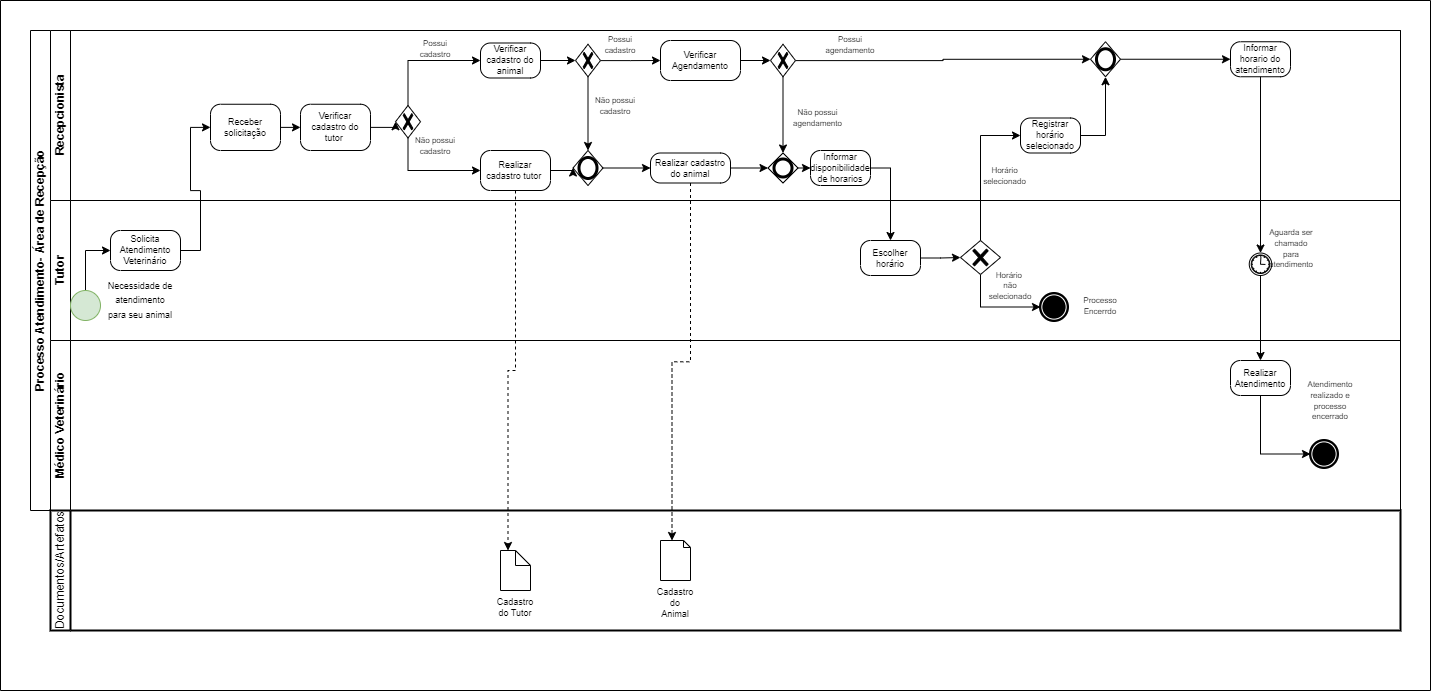
\includegraphics[width=0.9\textwidth]{images/fluxo de atendimento-rec.png}
        \label{fluxo-rec}
    \end{sidewaysfigure}  

    \subsection{ Atendimento Veterinário - Consulta}
    Processo de Consulta adaptado de \citeonline{Rabelo:2012},     

    
    Processos Antes da Consulta:

	\begin{itemize}
	    \item Sala de Atendimento:
            \begin{itemize}
                \item Veterinário abre sistema verifica qual animal será atendido.
                \item Acessa cadastro do animal que será atendido, com seus dados gerais e dados do tutor.
            \end{itemize}
	\end{itemize}

		
    \begin{itemize}
        \item Transição:
            \begin{itemize}
                \item Auxiliar encaminha animal e tutor pra sala de atendimento.
                \item Veterinário cria novo prontuário de atendimento (Caso seja retorno, clicar na opção retorno e \emph{linkar} com prontuário de atendimento inicial (para comparar evolução de quadro)).
            \end{itemize}
    \end{itemize}

    \begin{itemize}
        \item Início do Atendimento / Consulta 

        \begin{itemize}
            \item Auxiliar pesa animal e informa veterinário
            \item Veterinário insere peso no campo Peso do Prontuário.
            \item Veterinário preenche campo Queixa Principal.
            \item Veterinário preenche campo Anamnese 
            \item Veterinário realiza exame físico (Estado de consciência, Temperatura, FC, FR, Grau de Desidratação, TPC, Cor de mucosa, Sensibilidade/ Dor)
            \item Veterinário passa dados coletados para o Prontuário.
            \item Veterinário preenche campo Suspeita Diagnóstica.
            \item Veterinário preenche campo Exames, caso necessário, e marca retorno (Abre Agendamento?).
            \item Veterinário encaminha para medicação -> caso necessário e anota medicação utilizada.
            \item Veterinário preenche campo de Medicação utilizada e dose -> alerta para medicamentos controlados.
            \item Veterinário prescreve medicação para tutor, caso necessário, e preenche campo Prescrições.

        \end{itemize}
        \item Veterinário Finaliza Processo.
    \end{itemize}

	
  



     
    \section{Análise de Requisitos}

        Na etapa de análise de requisitos, a equipe passa a elaborar em maior nível de detalhamento as regras e características que a aplicação deve suportar, compreendendo de maneira mais assertiva as principais necessidades do cliente e definindo as prioridades do projeto.

        Esse é um processo evolutivo incremental em que a equipe deve se reunir com o \emph{Product} \emph{Owner} em frequência definida a fim de refinar os requisitos levantados para o andamento das histórias registradas como itens do \emph{product} \emph{backlog}. 

        Conforme as histórias são desenvolvidas, os membros da equipe criarão tarefas de acordo com o entendimento do refinamento discutido.

        Partindo das regras de negócio, são apresentados os requisitos funcionais, não funcionais e, por fim, as histórias de usuário.

         \subsection{Regras de Negócio}

            As regras de negócio são as premissas necessárias para a modelagem do projeto e através delas serão definidas as regras básicas as quais o sistema deve concernir.

            Tem por objetivo explicitar as restrições a serem adotadas pelo sistema a fim de garantir assertividade ao escopo definido para completude das ferramentas e histórias em desenvolvimento, bem como as interdependências entre as ferramentas e historias relacionadas.

            O Quadro \ref{tab:regra} dispõe das informações referente às regras de negócios do CertVet:

            \begin{center}
                \begin{quadro}[H]
                \caption{Regras de Negócio}
                \begin{tabulary}{1.0\textwidth}{|C|p{23em}|C|}
                \hline

                 Código & Descrição & Requisito Relacionado\\
                \hline
                RN01 & Somente usuário autenticado pode ter acesso ao sistema & RF01\\
                \hline
                RN02 & O usuário deve se autenticar informando seu e-mail e senha de cadastro. & RF02\\
                \hline
                RN03 & O usuário terá acesso às funcionalidades de acordo com \DIFdelbegin \DIFdel{o seu tipo de conta}\DIFdelend \DIFaddbegin \DIFadd{a permissão concedida pelo usuário administrador}\DIFaddend . & \\
                \hline
                RN04 & Apenas profissionais com número de CRMV válido devem ter acesso às funcionalidades clínicas. & \\
                \hline
                RN05 & Os prontuários digitais devem seguir o padrão dos modelos oficiais \citeonline {doc_obrig}. & \DIFdelbegin \DIFdel{RF10}\DIFdelend \DIFaddbegin \DIFadd{RF09}\DIFaddend \\
                \hline
                RN06 & Somente usuários com autorização podem realizar edições nos prontuários. & \DIFdelbegin \DIFdel{RF11}\DIFdelend \DIFaddbegin \DIFadd{RF10}\DIFaddend \\
                \hline
                RN07 & Na gestão de medicamentos, a retirada deve ser feita apenas por profissionais veterinários autorizados. & \DIFdelbegin \DIFdel{RF14 e RF15}\DIFdelend \DIFaddbegin \DIFadd{RF13 e RF14}\DIFaddend \\
                \hline
                RN08 & O controle de vacinação deve ser visível por todas as partes envolvidas, profissionais e tutores. & \DIFdelbegin \DIFdel{RF16, RF17 e RF18}\DIFdelend \DIFaddbegin \DIFadd{RF15, RF16 e RF17}\DIFaddend \\
                \hline
                \end{tabulary}   
                \label{tab:regra}
                \centering
                \footnotesize {Fonte: Elaborado pelos autores.}
                \end{quadro}
            \end{center}

        \subsection{Requisitos Funcionais}

            Nos Quadros \ref{tab:req_func} e \ref{tab:req_func2} são apresentados os requisitos funcionais, detalhando as necessidades e especificações das ações que o sistema deve executar, ignorando as limitações físicas, focando apenas no comportamento de entrada e saída do sistema.

            \begin{center}
                \begin{quadro}[H]
                \caption{Requisitos Funcionais}
                \begin{tabulary}{1.0\textwidth}{|p{5em}|p{8em}|p{18em}|}
                \hline
                Código & Requisito & Descrição\\
                \hline
                RF01 & Criar conta & O usuário deve criar uma conta de acordo com a sua ocupação (Veterinário | Auxiliar) e seus dados.\\
                \hline
                RF02 & Autenticar usuário & O sistema deve permitir que o usuário entre em sua conta já criada no sistema.\\
                \hline
                RF03 & Alterar senha & O sistema deve permitir que o usuário altere a sua senha.\\
                \hline
                RF04 & \DIFdelbegin \DIFdel{Redefinição de senha }%DIFDELCMD < & %%%
\DIFdel{O sistema deve permitir que o usuário solicite a redefinição de sua senha.}%DIFDELCMD < \\
%DIFDELCMD <                 \hline
%DIFDELCMD <                 %%%
\DIFdel{RF05 }%DIFDELCMD < & %%%
\DIFdelend Agendar consultas & O sistema deve permitir que o usuário autenticado agende consulta, informando data, horário, paciente e profissional responsável após verificar que este não possui nenhuma consulta já marcada no horário informado.\\
                \hline
                \DIFdelbegin \DIFdel{RF06 }\DIFdelend \DIFaddbegin \DIFadd{RF05 }\DIFaddend & Cancelar consulta & O sistema deve permitir que o usuário autenticado cancele uma consulta já agendada.\\
                \hline
                \DIFdelbegin \DIFdel{RF07 }\DIFdelend \DIFaddbegin \DIFadd{RF06 }\DIFaddend & Cadastrar tutor & O sistema deve permitir que o usuário autenticado cadastre os dados do tutor do paciente, permitindo também sua consulta e edição.\\
                \hline
                \DIFdelbegin \DIFdel{RF08 }\DIFdelend \DIFaddbegin \DIFadd{RF07 }\DIFaddend & Cadastrar animal & O sistema deve permitir que o usuário autenticado cadastre os dados do animal, permitindo também sua consulta e edição.\\
                \hline
                \DIFdelbegin \DIFdel{RF09 }\DIFdelend \DIFaddbegin \DIFadd{RF08 }\DIFaddend & Visualizar histórico de consultas & O sistema deve permitir que todos os usuários consultem o histórico de consultas já realizadas, informando dados do paciente.\\
                \hline
                \DIFdelbegin \DIFdel{RF10 }\DIFdelend \DIFaddbegin \DIFadd{RF09 }\DIFaddend & Criar prontuário & O sistema deve permitir que o veterinário crie o prontuário digital de atendimento do paciente.\\
                \hline
                \DIFdelbegin \DIFdel{RF11 }\DIFdelend \DIFaddbegin \DIFadd{RF10 }\DIFaddend & Editar prontuário de atendimento & O sistema deve permitir que o veterinário edite informações específicas do prontuário digital de atendimento do paciente.\\
                \hline
                \DIFdelbegin \DIFdel{RF12 }\DIFdelend \DIFaddbegin \DIFadd{RF11 }\DIFaddend & Verificar histórico de alterações \DIFdelbegin \DIFdel{no prontuário }\DIFdelend \DIFaddbegin \DIFadd{nos documentos }\DIFaddend & O sistema deve permitir que todos os usuários consultem o histórico de alterações feitas \DIFdelbegin \DIFdel{no prontuário digital de atendimento do paciente}\DIFdelend \DIFaddbegin \DIFadd{nos documentos digitais}\DIFaddend .\\
                \hline

                \end{tabulary}
                \label{tab:req_func}
                \centering

                \footnotesize {Fonte: Elaborado pelos autores.}
                \end{quadro}
            \end{center}   

            \begin{center}
                \begin{quadro}[h]
                \caption{Requisitos Funcionais - continuação}
                \begin{tabulary}{1.0\textwidth}{|p{5em}|p{8em}|p{18em}|}
                \hline
                Código & Requisito & Descrição\\
                \hline
                \DIFdelbegin \DIFdel{RF13 }\DIFdelend \DIFaddbegin \DIFadd{RF12 }\DIFaddend & Visualizar aspectos hereditários & O sistema deve permitir que seja visível, ao usuário autenticado, o histórico de aspectos hereditários do animal, quando este possuí-lo.\\
                \hline
                \DIFdelbegin \DIFdel{RF14 }\DIFdelend \DIFaddbegin \DIFadd{RF13 }\DIFaddend & Registar consumo de medicamento & O sistema deve permitir que o veterinário autorizado registre o uso de medicamento no prontuário digital do paciente, quando usado no atendimento.\\
                \hline
                \DIFdelbegin \DIFdel{RF15 }\DIFdelend \DIFaddbegin \DIFadd{RF14 }\DIFaddend & Visualizar histórico de medicamento & O sistema deve permitir que o usuário consulte o histórico do uso de medicamento, quando usado no atendimento.\\
                \hline
                \DIFdelbegin \DIFdel{RF16 }\DIFdelend \DIFaddbegin \DIFadd{RF15 }\DIFaddend & Aplicar vacina & O sistema deve permitir que o veterinário preencha o prontuário específico para vacinação do paciente e que os dados sejam inseridos na ficha do animal.\\
                \hline
                \DIFdelbegin \DIFdel{RF17 }\DIFdelend \DIFaddbegin \DIFadd{RF16 }\DIFaddend & Visualizar \DIFdelbegin \DIFdel{carteirinha }\DIFdelend \DIFaddbegin \DIFadd{histórico }\DIFaddend de vacinação & O sistema deve permitir a visualização das vacinas já aplicadas no paciente.\\
                \hline
                \DIFdelbegin \DIFdel{RF18 }\DIFdelend \DIFaddbegin \DIFadd{RF17 }\DIFaddend & Visualizar vacinas agendadas & O sistema deve permitir visualização das vacinas agendadas para aplicação no paciente.\\
                \hline
                \end{tabulary}
                \label{tab:req_func2}
                \centering

                \footnotesize {Fonte: Elaborado pelos autores.}
                \end{quadro}
            \end{center}
        \DIFdelbegin %DIFDELCMD < 

%DIFDELCMD <         %%%
\DIFdelend %DIF >  Remover RF12 após conversa com os profes. Incluir que a CertVet compreende diferentes perfis de usuário gerenciados pelo usuário administrador da clínica %
        \subsection{Requisitos não Funcionais}

            Os requisitos não funcionais tratam-se de restrições mais técnicas do projeto, são as necessidades que não são atendidas necessariamente através de funcionalidades, objetivando garantir níveis satisfatórios  de desempenho, disponibilidade, escalabilidade, dentre outras garantias que permitam a máxima usabilidade do sistema. Os requisitos não funcionais que compreendem à CertVet são elencados no Quadro \ref{tab:req_nfunc}.

            \begin{center}
                \begin{quadro}[h]
                  \caption{Requisitos Não Funcionais}
                \begin{tabulary}{1.0\textwidth}{|C|p{25em}|p{7em}|}
                \hline
                Código & Requisito & Categoria\\
                \hline
                RNF01 & O sistema deve estar disponível para o usuário de acordo com o funcionamento da clínica, podendo ser utilizado 24 horas por dia, 7 dias por semana, com tolerância de 0,1\% de falhas. & Disponibilidade\\
                \hline
                RNF02 & O sistema deve ser implementado de forma que seja apto para crescimento, visando suportar a entrada de novos usuários e novas funcionalidades, sem comprometer seu desempenho e segurança. & Escalabilidade, Portabilidade\\
                \hline
                RNF03 & O sistema deve atender ao Artigo 8 da Lei nº 5.517, prevendo a fiscalização do exercício profissional pelos Conselhos Federal e Regionais de Medicina Veterinária. & Legalidade\\
                \hline
                RNF04 & As documentações criadas e utilizadas no sistema devem seguir a padronização de elaboração, fornecimento e guarda, conforme Resolução 1071/2014, também do Conselho Federal de Medicina Veterinária. & Legalidade\\
                \hline
                RNF05 & O sistema deve atender às especificações da Lei Geral de Proteção de Dados (Lei 13.709/18), garantindo a segurança dos dados dos usuários, animais e tutores. & Legalidade\\
                \hline
                RNF06 & O sistema deve ter sua interface organizada de forma que o usuário consiga utilizar suas funcionalidades sem dificuldades de operá-las. & Usabilidade\\
                \hline
                RNF07 & O sistema deve compreender tecnologia de internacionalização, a fim de promover sua tradução para diferentes idiomas. & Usabilidade\\
                \hline
                RNF08 & O sistema deve contar com um protocolo criptografado e seguro de transferência de dados em sua implementação. & Segurança\\
                \hline
                RNF09 & O sistema deve apresentar um layout que seja adaptável para as dimensões de tela de diferentes dispositivos, garantindo responsividade. & Usabilidade\\
                \hline
                \end{tabulary}
                \label{tab:req_nfunc}
                \centering

               \footnotesize Fonte: Elaborado pelos autores.
                \end{quadro}
            \end{center}

\subsection{Histórias de Usuários}

    
    \begin{center}
        \begin{quadro}[H]
        \caption{Histórias de Usuário}
        \begin{tabulary}{1.0\textwidth}{|p{5em}|p{8em}|p{18em}|}
        \hline
        Código & História & Descrição\\
        \hline
        HU-01 & Função gerar documento com assinatura digital/certificação & Eu como usuário autorizado, quero gerar um documento oficial com assinatura digital, que me permita rastrear todas suas versões anteriores, para que sejam rastreáveis e passíveis de identificação.\\
        \hline
        HU-02 & Função preencher prontuário & Eu como usuário autorizado, quero preencher um prontuário para um animal em atendimento, para que seus dados sejam salvos.\\
        \hline
        HU-03 & Função salvar prontuário & Eu como usuário autorizado, quero salvar o prontuário digital, para que seja possível sua leitura em momento posterior.\\
        \hline
        HU-04 & Função uso de medicamentos controlados & Eu como usuário autorizado, quero anotar os medicamentos controlados utilizados no atendimento, para que seja possível seu controle com os dados do estoque.\\
        \hline
        HU-05 & Função inserir medicamentos no estoque & Eu, como usuário autorizado, quero inserir no sistema a quantidade total de produtos no estoque, para que seja possível o controle de quantidade usada por atendimento, perdida e que ainda está disponível.\\
        \hline
        HU-06 & Função visualizar prontuários & Eu, como usuário autorizado, quero acessar os prontuários de determinado animal, para que seja possível acompanhar seu histórico ou quadro clínico.\\
        \hline
        HU-07 & Função salvar dados hereditários &  Eu, como usuário autorizado, quero inserir dados sobre pais e descendentes (quando existentes), na ficha médica do animal, para que tais dados estejam disponíveis para consulta quando necessário.\\
        \hline
        HU-08 &  Função recuperar aspectos hereditários &  Eu, como usuário autorizado, quero consultar aspectos hereditários do animal (quando disponível), para obter informações úteis ao tratamento do mesmo.\\
        \hline
        HU-09 & Função inserir dados na agenda & Eu, como funcionário, quero inserir dados de um atendimento na agenda, para que os atendimentos futuros sejam planejados.\\
        \hline
        HU-10 & Função cadastrar cliente & Eu, como funcionário, quero cadastrar um cliente no sistema, para que seus dados estejam disponíveis para uso dentro da clínica\\
        \hline
        \end{tabulary}

        \label{tab:hist_usuario}
        \centering
        {\footnotesize Fonte: Elaborado pelos autores.}
        \end{quadro}
    \end{center}  

    \section{Modelagem}

        \subsection{Modelo Entidade Relacionamento}

            \begin{figure}[H]
            \centering
                \caption{Modelo Entidade Relacionamento}
                \DIFdelbeginFL %DIFDELCMD < 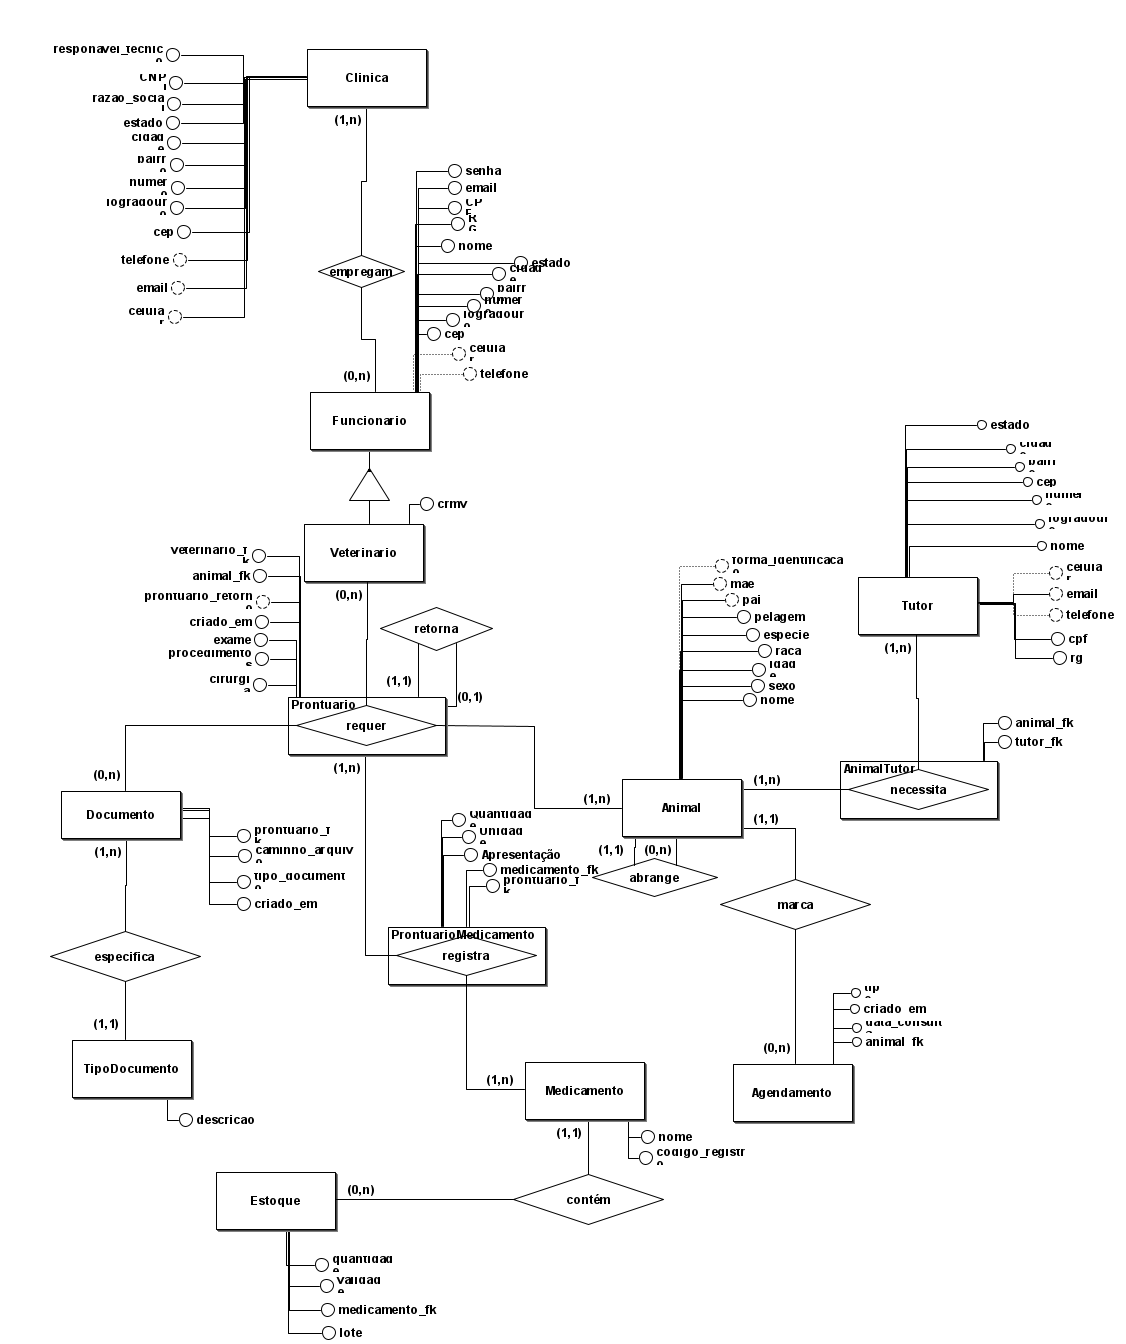
\includegraphics[ width=\linewidth]{images/ProjetoPI1.2 .png}
%DIFDELCMD <                 %%%
\DIFdelendFL \DIFaddbeginFL 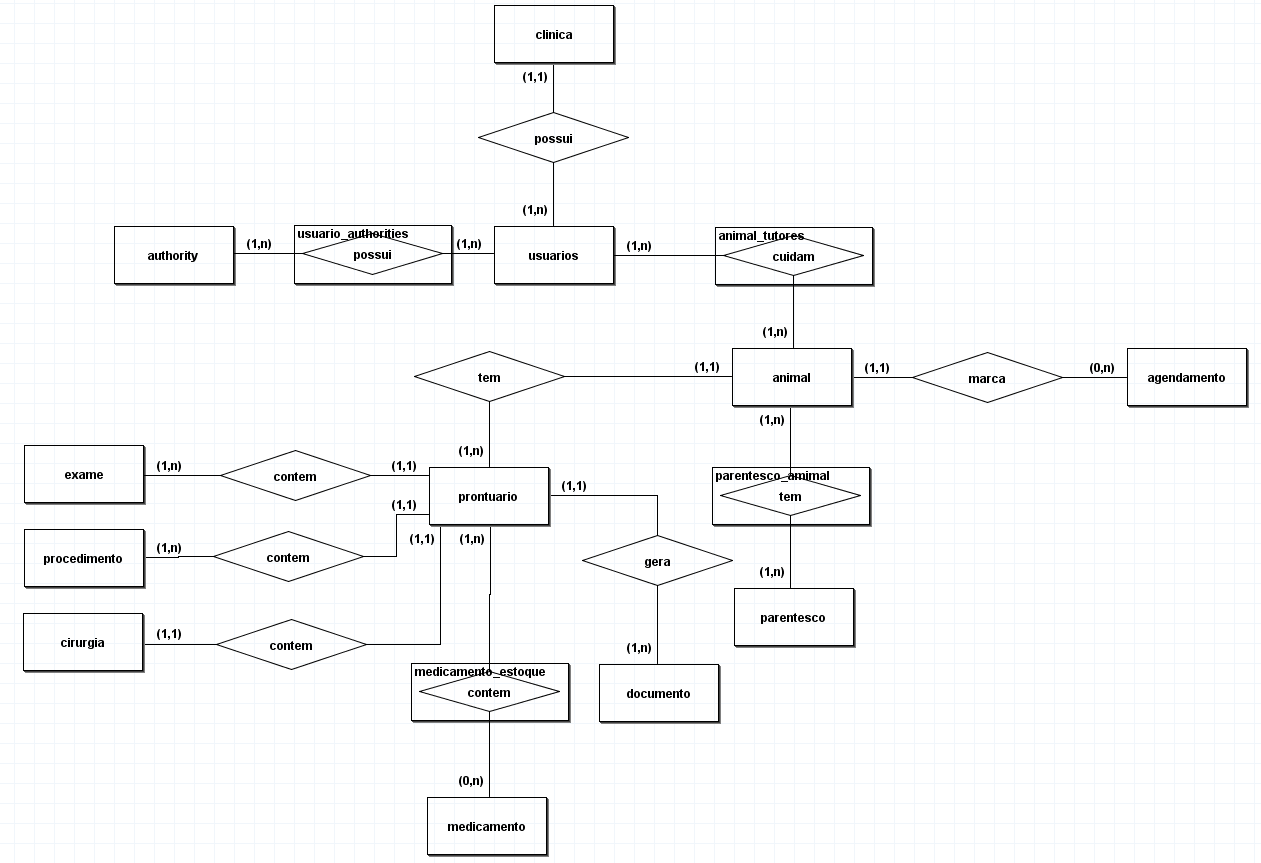
\includegraphics[ width=\linewidth]{images/ProjetoPI1.2.v2.png}
                \DIFaddendFL 

                \DIFdelbeginFL %DIFDELCMD < \label{fig:MER}
%DIFDELCMD <                 %%%
\DIFdelendFL \DIFaddbeginFL \label{fig:MER2}
                \DIFaddendFL \centering
                {\footnotesize Fonte: Elaborado pelos autores.}
            \end{figure}

            \begin{center}
                \begin{quadro}[H]
                \centering
                \caption{Entidades do \nameref{fig:MER} }
                \begin{tabulary}{1.0\textwidth}{|p{10em}|p{26em}|}
                \hline
                Entidade & Descrição\\
                \hline
                Prontuário & Entidade em que é armazenado os dados do atendimento de um animal. \\
                \hline
                Veterinário & Entidade em que é armazenado os dados do profissional veterinário.\\
                \hline
                Animal & Entidade em que é armazenado os dados do animal.\\
                \hline
                Medicamento & Entidade em que é armazenado os dados do medicamento.\\
                \hline
                ProntuárioMedicamento & Entidade em que é associado o medicamente com a quantidade utilizada no atendimento.\\
                \hline
                Estoque & Entidade que armazena a quantidade disponível do medicamento.\\
                \hline
                Clínica & Entidade que armazena dados referentes ao estabelecimento veterinário.\\
                \hline
                Tutor & Entidade que armazena dados do tutor/proprietário do animal atendido.\\
                \hline
                AnimalTutor & Entidade que associa um animal com seu tutor.\\
                \hline
                Agendamento & Entidade que registra um animal com horario de atendimento, clínica e tipo de atendimento.\\
                \hline
                Funcionário & Entidade que armazena os dados dos funcionários do estabelecimento.\\
                \hline
                Documento & Entidade que armazena dados comuns referentes a documentos obrigatórios gerados pelo veterinário.\\
                \hline
                TipoDocumento & Entidade que armazena dados específicos de um documento obrigatório.\\
                \hline
                \end{tabulary}
                \label{tab: entidades} \\
                \centering
                {\footnotesize Fonte: Elaborado pelos autores.}
                \end{quadro}
            \end{center}  

    %DIF >          \begin{center}
    %DIF >            \begin{quadro}[H]
            \DIFaddbegin 

    %DIF >              \caption{Dicionário de Dados - Prontuário}
    %DIF >              \begin{tabulary}{1.0\textwidth}{|p{9em}|c|c|c|p{19em}|}
    %DIF >              \hline
    %DIF >              Atributos & Chave & NN & Tipo & Descrição\\
    %DIF >              \hline
    %DIF >              Veterinário & FK & x & bigint & Identifica o veterinário responsável \\
    %DIF >              \hline
    %DIF >              Animal & FK & x & bigint & Identifica o animal atendido \\
    %DIF >              \hline
    %DIF >              Prontuário_retorno & x & x & boolean & Identifica se o prontuário é de um retorno\\
    %DIF >              \hline
    %DIF >              Criado Em & x & x & timestamp & registro de quando o prontuário foi feito \\
    %DIF >              \hline
    %DIF >              Exame & x & x & varchar & Campo para especificar Exames solicitados\\
    %DIF >              \hline
    %DIF >              Procedimento & x & x & varchar & Campo para especificar procedimentos realizados \\
    %DIF >              \hline
    %DIF >              Cirurgia & x & x & varchar & Campo para especificar quando há necessidade de cirurgia\\
    %DIF >              \hline
    %DIF >              Prontuário & PK & x & bigint & Identificação do prontuário \\
    %DIF >              \hline
    %DIF >              \end{tabulary}
    %DIF >              \label{qd: md-prontuario}
    %DIF >              \centering
    %DIF >              \footnotesize Fonte: Elaborado pelos autores.
    %DIF >              \end{quadro}
    %DIF >              \end{center}

    %DIF >          \begin{center}
    %DIF >            \begin{quadro}[H]
    %DIF >            \centering
    %DIF >                \caption{Dicionário de Dados - Veterinário}
    %DIF >                \begin{tabulary}{1.0\textwidth}{|p{9em}|c|c|c|p{19em}|}
    %DIF >              \hline
    %DIF >              Atributos & Chave & NN & Tipo & Descrição\\
    %DIF >              \hline
    %DIF >              ID & PK & x & BIGINT & Atributo de Identificação do médico veterinário \\
    %DIF >              \hline
    %DIF >              CRMV & - & x & varchar & Atributo que guarda o registro do médico veterinário\\
    %DIF >              \hline
    %DIF >              \end{tabulary}

    %DIF >                \label{qd: md-veterinario}
    %DIF >                \centering
    %DIF >      {\footnotesize Fonte: Elaborado pelos autores.}
    %DIF >            \end{quadro}
    %DIF >          \end{center}

    %DIF >          \begin{center}
    %DIF >            \begin{quadro}[H]
    %DIF >            \centering
    %DIF >                \caption{Dicionário de Dados - Animal}
    %DIF >                \begin{tabulary}{1.0\textwidth}{|p{9em}|c|c|c|p{19em}|}
    %DIF >              \hline
    %DIF >              Atributos & Chave & NN & Tipo & Descrição\\
    %DIF >              \hline
    %DIF >              ID & PK & x & BIGINT & Identifica a chave do \\
    %DIF >              \hline
    %DIF >              Nome & - & x & varchar & Atributo que guarda o nome do animal\\
    %DIF >              \hline
    %DIF >              Espécie & - & x & varchar & Atributo que recebe a especie do animal\\
    %DIF >              \hline
    %DIF >              Raça & - & x & varchar & Atributo que recebe a raça do animal \\
    %DIF >              \hline
    %DIF >              Sexo & - & x & varchar & Atributo que recebe o sexo do animal\\
    %DIF >              \hline
    %DIF >              Idade & - & x & BIGINT & Atributo que recebe a idade do animal\\
    %DIF >              \hline
    %DIF >              Pelagem & - & - & varchar & Atributo que recebe o tipo de pelagem do animal \\
    %DIF >              \hline
    %DIF >              Forma\_identificação & - & - & varchar & Atributo que recebe a identificação do animal\\
    %DIF >              \hline
    %DIF >              Mãe & FK & - & BIGINT & Atributo que identifica a mãe do animal \\
    %DIF >              \hline
    %DIF >              Pai & FK & - & BIGINT & Atributo que identifica o pai do animal \\
    %DIF >              \hline
    %DIF >              \end{tabulary}

    %DIF >                \label{qd: md-animal}
    %DIF >                \centering
    %DIF >      {\footnotesize Fonte: Elaborado pelos autores.}
    %DIF >            \end{quadro}
    %DIF >          \end{center}

    %DIF >  \begin{center}
    %DIF >    \begin{quadro}[H]
    %DIF >    \centering
    %DIF >        \caption{Dicionário de Dados - Medicamento}
    %DIF >        \begin{tabulary}{1.0\textwidth}{|p{9em}|c|c|c|p{19em}|}
    %DIF >      \hline
    %DIF >      Atributos & Chave & NN & Tipo & Descrição\\
    %DIF >      \hline
    %DIF >      Id & PK & x & BIGINT & Atributo que identifica o medicamento\\
    %DIF >      \hline
    %DIF >      Código\_Registro & - & x & BIGINT & Atributo que identifica o código do medicamento\\
    %DIF >      \hline
    %DIF >      Nome & - & x & varchar & Atributo que identifica o nome do medicamento\\
    %DIF >      \hline
    %DIF >      \end{tabulary}

    %DIF >        \label{qd: md-medicamento}
    %DIF >        \centering
    %DIF >      {\footnotesize Fonte: Elaborado pelos autores.}
    %DIF >    \end{quadro}
    %DIF >  \end{center}

    %DIF >  \begin{center}
    %DIF >    \begin{quadro}[H]
    %DIF >    \centering
    %DIF >        \caption{Dicionário de Dados - ProntuárioMedicamento}
    %DIF >        \begin{tabulary}{1.0\textwidth}{|p{9em}|c|c|c|p{19em}|}
    %DIF >      \hline
    %DIF >      Atributos & Chave & NN & Tipo & Descrição\\
    %DIF >      \hline
    %DIF >      Prontuário & FK & x & BIGINT & Identificação do Prontuário \\
    %DIF >      \hline
    %DIF >      Medicação & FK & x & BIGINT & Atributo que identifica o medicamento utilizado \\
    %DIF >      \hline
    %DIF >      Apresentação & - & x & varchar & Atributo que recebe o tipo de apresentação do medicamento\\
    %DIF >      \hline
    %DIF >      Quantidade & - & x & BIGINT & Atributo que recebe a quantidade do medicamento utilizada\\
    %DIF >      \hline
    %DIF >      Unidade & - & x & varchar & Atributo que recebe a unidade do medicamento \\
    %DIF >      \hline
    %DIF >      \end{tabulary}

    %DIF >        \label{qd: md-prontuariomedicamento}
    %DIF >        \centering
    %DIF >      {\footnotesize Fonte: Elaborado pelos autores.}
    %DIF >    \end{quadro}
    %DIF >  \end{center}

    %DIF >  \begin{center}
    %DIF >    \begin{quadro}[H]
    %DIF >    \centering
    %DIF >        \caption{Dicionário de Dados - Estoque}
    %DIF >        \begin{tabulary}{1.0\textwidth}{|p{9em}|c|c|c|p{19em}|}
    %DIF >      \hline
    %DIF >      Atributos & Chave & NN & Tipo & Descrição\\
    %DIF >      \hline
    %DIF >      Medicamento & FK & x & BIGINT & Atributo que identifica o medicamento\\
    %DIF >      \hline
    %DIF >      Lote & - & x & BIGINT & Atributo que recebe o lote do medicamento\\
    %DIF >      \hline
    %DIF >      Validade & - & x & timestamp & Atributo que recebe a data de validade do medicamento \\
    %DIF >      \hline
    %DIF >      Quantidade & - & x & BIGINT & Atributo que recebe a quantidade de medicamento total do estoque \\
    %DIF >      \hline
    %DIF >      \end{tabulary}

    %DIF >        \label{qd: md-estoque}
    %DIF >        \centering
    %DIF >      {\footnotesize Fonte: Elaborado pelos autores.}
    %DIF >    \end{quadro}
    %DIF >  \end{center}

    %DIF >  \begin{center}
    %DIF >    \begin{quadro}[H]
    %DIF >    \centering
    %DIF >        \caption{Dicionário de Dados - Clínica}
    %DIF >        \begin{tabulary}{1.0\textwidth}{|p{9em}|c|c|c|p{19em}|}
    %DIF >      \hline
    %DIF >      Atributos & Chave & NN & Tipo & Descrição\\
    %DIF >      \hline
    %DIF >      ID & PK & x & BIGINT & Atributo que identifica a clínica \\
    %DIF >      \hline
    %DIF >      Razao Social & - & x & varchar & Atributo que guarda o nome da clínica\\
    %DIF >      \hline
    %DIF >      CNPJ & - & x & BIGINT & Atributo que guarda o CNPJ da clínica \\
    %DIF >      \hline
    %DIF >      Responsável Técnico & FK & x & varchar & Atributo que recebe o nome do funcionario veterinário cadastrado como RT\\
    %DIF >      \hline
    %DIF >      Telefone & - & x & varchar & Atributo que recebe o telefone da clínica\\
    %DIF >      \hline
    %DIF >      Email & - & x & varchar & Atributo que recebe o email da clínica\\
    %DIF >      \hline
    %DIF >      Celular & - & x & varchar & Atributo que recebe o celular da clínica \\
    %DIF >      \hline
    %DIF >      Estado & - & x & varchar & Atributo que recebe o estado da clínica\\
    %DIF >      \hline
    %DIF >      Cidade & - & x & varchar & Atributo que recebe a cidade da clínica \\
    %DIF >      \hline
    %DIF >      Bairro & - & x & varchar & Atributo que recebe o bairro da clínica \\
    %DIF >      \hline
    %DIF >      Logradouro & - & x & varchar & Atributo que recebe o nome da rua da clínica\\
    %DIF >      \hline
    %DIF >      Número & - & x & varchar & Atributo que recebe o número da clínica \\
    %DIF >      \hline
    %DIF >      CEP & - & x & varchar &  Atributo que recebe o CEP da clinica\\
    %DIF >      \hline
    %DIF >      \end{tabulary}

    %DIF >        \label{qd: md-clinica}
    %DIF >        \centering
    %DIF >      {\footnotesize Fonte: Elaborado pelos autores.}
    %DIF >    \end{quadro}
    %DIF >  \end{center}

    %DIF >  \begin{center}
    %DIF >    \begin{quadro}[H]
    %DIF >    \centering
    %DIF >        \caption{Dicionário de Dados - Tutor}
    %DIF >        \begin{tabulary}{1.0\textwidth}{|p{9em}|c|c|c|p{19em}|}
    %DIF >      \hline
    %DIF >      Atributos & Chave & NN & Tipo & Descrição\\
    %DIF >      \hline
    %DIF >      ID & PK & x & BIGINT & Atributo que identifica o tutor \\
    %DIF >      \hline
    %DIF >      Nome & - & x & varchar & Atributo que guarda o nome do tutor\\
    %DIF >      \hline
    %DIF >      Rg & - & x & varchar & Atributo que recebe o rg do tutor \\
    %DIF >      \hline
    %DIF >      CPF & - & x & varchar & Atributo que recebe o CPF do tutor\\
    %DIF >      \hline
    %DIF >      Email & - & x & varchar & Atributo que recebe o email do tutor\\
    %DIF >      \hline
    %DIF >      Telefone & - & x & varchar & Atributo que recebe o telefone do tutor\\
    %DIF >      \hline
    %DIF >      Celular & - & x & varchar & Atributo que recebe o celular do tutor\\
    %DIF >      \hline
    %DIF >      Estado & - & x & varchar & Atributo que recebe o estado do tutor\\
    %DIF >      \hline
    %DIF >      Cidade & - & x & varchar & Atributo que recebe a cidade do tutor\\
    %DIF >      \hline
    %DIF >      Bairro & - & x & varchar & Atributo que recebe o bairro do tutor\\
    %DIF >      \hline
    %DIF >      Logradouro & - & x & varchar & Atributo que recebe o nome da rua do tutor\\
    %DIF >      \hline
    %DIF >      Numero & - & x & varchar & Atributo que recebe o numero de residencia do tutor\\
    %DIF >      \hline
    %DIF >      CEP & - & x & varchar & Atributo que recebe o CEP do tutor\\
    %DIF >      \hline
    %DIF >      \end{tabulary}

    %DIF >        \label{qd: md-tutor}
    %DIF >        \centering
    %DIF >      {\footnotesize Fonte: Elaborado pelos autores.}
    %DIF >    \end{quadro}
    %DIF >  \end{center}

    %DIF >  \begin{center}
    %DIF >    \begin{quadro}[H]
    %DIF >    \centering
    %DIF >        \caption{Dicionário de Dados - AnimalTutor}
    %DIF >        \begin{tabulary}{1.0\textwidth}{|p{9em}|c|c|c|p{19em}|}
    %DIF >      \hline
    %DIF >      Atributos & Chave & NN & Tipo & Descrição\\
    %DIF >      \hline
    %DIF >      Tutor & FK & x & BIGINT & Atributo que identifica o tutor. \\
    %DIF >      \hline
    %DIF >      Animal & FK & x & BIGINT & Atributo que identifica o animal.\\
    %DIF >      \hline
    %DIF >      \end{tabulary}

    %DIF >        \label{qd: md-animaltutor}
    %DIF >        \centering
    %DIF >      {\footnotesize Fonte: Elaborado pelos autores.}
    %DIF >    \end{quadro}
    %DIF >  \end{center}

    %DIF >  \begin{center}
    %DIF >    \begin{quadro}[H]
    %DIF >    \centering
    %DIF >        \caption{Dicionário de Dados - Agendamento}
    %DIF >        \begin{tabulary}{1.0\textwidth}{|p{9em}|c|c|c|p{19em}|}
    %DIF >      \hline
    %DIF >      Atributos & Chave & NN & Tipo & Descrição\\
    %DIF >      \hline
    %DIF >      %ID & PK & x & BIGINT & Atributo que identifica o agendamento \\
    %DIF >      |%\hline
    %DIF >      Animal & FK & x & BIGINT & Atributo que identifica o animal que passará por atendimento \\
    %DIF >      \hline
    %DIF >      Tipo & - & x & varchar & Atributo que recebe o tipo de atendimento será realizado \\
    %DIF >      \hline
    %DIF >      Criado\_Em & - & x & timestamp & Atributo que guarda a data quando foi realizado o agendamento\\
    %DIF >      \hline
    %DIF >      Data\_Consulta & - & x & timestamp & Atributo que guarda a data a ser realizado o atendimento \\
    %DIF >      \hline
    %DIF >      \end{tabulary}

    %DIF >        \label{qd: md-agendamento}
    %DIF >        \centering
    %DIF >      {\footnotesize Fonte: Elaborado pelos autores.}
    %DIF >    \end{quadro}
    %DIF >  \end{center}

    %DIF >  \begin{center}
    %DIF >    \begin{quadro}[H]
    %DIF >    \centering
    %DIF >        \caption{Dicionário de Dados - Funcionário}
    %DIF >        \begin{tabulary}{1.0\textwidth}{|p{9em}|c|c|c|p{19em}|}
    %DIF >      \hline
    %DIF >      Atributos & Chave & NN & Tipo & Descrição\\
    %DIF >      \hline
    %DIF >      ID & PK & x & BIGINT & Atributo que identifica o funcionário no sistema \\
    %DIF >      \hline
    %DIF >      Nome & - & x & varchar & Atributo que recebe o nome do funcionário \\
    %DIF >      \hline
    %DIF >      RG & - & x & varchar & Atributo que recebe o RG do funcionário\\
    %DIF >      \hline
    %DIF >      CPF & - & x & varchar & Atributo que recebe o CPF do funcionário\\
    %DIF >      \hline
    %DIF >      Senha & - & x & varchar & Atributo da senha de acesso do funcionário ao sistema\\
    %DIF >      \hline
    %DIF >      Telefone & - & - & varchar & Atributo que recebe o contato telefônico do funcionário\\
    %DIF >      \hline
    %DIF >      Celular & - & x & varchar & Atributo que recebe o contato móvel do funcionário \\
    %DIF >      \hline
    %DIF >      Email & - & x & varchar & Atributo que recebe o endereço eletrônico do funcionário\\
    %DIF >      \hline
    %DIF >      Estado & - & - & varchar & Atributo que recebe o estado da residência do funcionário\\
    %DIF >      \hline
    %DIF >      Cidade & - & - & varchar & Atributo que recebe a cidade da residência do funcionário\\
    %DIF >      \hline
    %DIF >      Bairro & - & - & varchar & Atributo que recebe o bairro da residência do funcionário\\
    %DIF >      \hline
    %DIF >      Logradouro & - & - & varchar & Atributo que recebe a rua da residência do funcinário \\
    %DIF >      \hline
    %DIF >      Número & - & - & int & Atributo que recebe a numeração da residencia do funcionário\\
    %DIF >      \hline
    %DIF >      CEP & - & - & varchar & Atributo que recebe o CEP do funcionário\\
    %DIF >      \hline
    %DIF >      \end{tabulary}

    %DIF >        \label{qd: md-funcionario}
    %DIF >        \centering
    %DIF >      {\footnotesize Fonte: Elaborado pelos autores.}
    %DIF >    \end{quadro}
    %DIF >  \end{center}

    %DIF >  \begin{center}
    %DIF >    \begin{quadro}[H]
    %DIF >    \centering
    %DIF >        \caption{Dicionário de Dados - Documento}
    %DIF >        \begin{tabulary}{1.0\textwidth}{|p{9em}|c|c|c|p{19em}|}
    %DIF >      \hline
    %DIF >      Atributos & Chave & NN & Tipo & Descrição\\
    %DIF >      \hline
    %DIF >      Prontuário & FK & x & BIGINT & Identificação do Prontuário \\
    %DIF >      \hline
    %DIF >      Tipo\_Documento & FK & x & BIGINT & Atributo que identifica tipo  de autorização \\
    %DIF >      \hline
    %DIF >      Caminho\_Arquivo & - & x & varchar & identifica a url do arquivo na AWS\\
    %DIF >      \hline
    %DIF >      Criado\_Em & - & x & timestamp & Atributo que identifica a data de criação do documento\\
    %DIF >      \hline
    %DIF >      \end{tabulary}

    %DIF >        \label{qd: md-documento}
    %DIF >        \centering
    %DIF >      {\footnotesize Fonte: Elaborado pelos autores.}
    %DIF >    \end{quadro}
    %DIF >  \end{center}

    %DIF >  \begin{center}
    %DIF >    \begin{quadro}[H]
    %DIF >    \centering
    %DIF >        \caption{Dicionário de Dados - TipoDocumento}
    %DIF >        \begin{tabulary}{1.0\textwidth}{|p{9em}|c|c|c|p{19em}|}
    %DIF >      \hline
    %DIF >      Atributos & Chave & NN & Tipo & Descrição\\
    %DIF >      \hline
    %DIF >      ID & PK & x & BIGINT & Atributo que identifica o documento\\
    %DIF >      \hline
    %DIF >      Descrição & - & - & varchar & Descreve qual tipo de documento\\
    %DIF >      \hline
    %DIF >      \end{tabulary}

    %DIF >        \label{qd: md-tipodocumento}
    %DIF >        \centering
    %DIF >      {\footnotesize Fonte: Elaborado pelos autores.}
    %DIF >    \end{quadro}
    %DIF >  \end{center}  

%       \DIFaddend \begin{center}
%       \begin{quadro}[H]
%       \DIFdelbegin %DIFDELCMD < 

% %DIFDELCMD <                 %%%
% \DIFdelend \DIFaddbegin \centering
%           \DIFaddend \caption{Dicionário de Dados - \DIFdelbegin \DIFdel{Prontuário}\DIFdelend \DIFaddbegin \DIFadd{Clinica}\DIFaddend }
%           \begin{tabulary}{1.0\textwidth}{|p{9em}|c|c|c|p{19em}|}
%         \hline
%         Atributos & Chave & NN & Tipo & Descrição\\
%         \hline
%         \DIFdelbegin \DIFdel{Veterinário }\DIFdelend \DIFaddbegin \DIFadd{ID }\DIFaddend & \DIFdelbegin \DIFdel{FK }\DIFdelend \DIFaddbegin \DIFadd{PK }\DIFaddend & x & \DIFdelbegin \DIFdel{bigint }\DIFdelend \DIFaddbegin \DIFadd{BIGINT }\DIFaddend & \DIFdelbegin \DIFdel{Identifica o veterinário responsável }\DIFdelend \DIFaddbegin \DIFadd{Atributo que identifica a clínica }\DIFaddend \\
%         \hline
%         \DIFdelbegin \DIFdel{Animal }\DIFdelend \DIFaddbegin \DIFadd{Razao Social }\DIFaddend & \DIFdelbegin \DIFdel{FK }\DIFdelend \DIFaddbegin \DIFadd{- }\DIFaddend & x & \DIFdelbegin \DIFdel{bigint }\DIFdelend \DIFaddbegin \DIFadd{varchar }\DIFaddend & \DIFdelbegin \DIFdel{Identifica o animal atendido }\DIFdelend \DIFaddbegin \DIFadd{Atributo que guarda o nome oficial do empreendimento no registro}\DIFaddend \\
%         \hline
%         \DIFdelbegin \DIFdel{Prontuário_retorno }\DIFdelend \DIFaddbegin \DIFadd{Nome Fantasia }\DIFaddend & \DIFaddbegin \DIFadd{- }& \DIFaddend x & \DIFaddbegin \DIFadd{varchar }& \DIFadd{Atributo que guarda o nome público da clínica}\\
%         \hline
%         \DIFadd{CNPJ }& \DIFadd{- }& \DIFaddend x & \DIFdelbegin \DIFdel{boolean }\DIFdelend \DIFaddbegin \DIFadd{BIGINT }\DIFaddend & \DIFdelbegin \DIFdel{Identifica se o prontuário é de um retorno}\DIFdelend \DIFaddbegin \DIFadd{Atributo que guarda o CNPJ da clínica }\DIFaddend \\
%         \hline
%         \DIFdelbegin \DIFdel{Criado Em }\DIFdelend %DIF > Responsável Técnico & FK & x & varchar & Atributo que recebe o nome do funcionario veterinário cadastrado como RT\\
%         \DIFaddbegin \DIFadd{Telefone }\DIFaddend & \DIFaddbegin \DIFadd{- }& \DIFaddend x & \DIFaddbegin \DIFadd{varchar }& \DIFadd{Atributo que recebe o telefone da clínica}\\
%         \hline
%         \DIFadd{Email }& \DIFadd{- }& \DIFaddend x & \DIFdelbegin \DIFdel{timestamp }\DIFdelend \DIFaddbegin \DIFadd{varchar }\DIFaddend & \DIFdelbegin \DIFdel{registro de quando o prontuário foi feito }\DIFdelend \DIFaddbegin \DIFadd{Atributo que recebe o email da clínica}\DIFaddend \\
%         \hline
%         \DIFdelbegin \DIFdel{Exame }\DIFdelend \DIFaddbegin \DIFadd{Celular }\DIFaddend & \DIFaddbegin \DIFadd{- }& \DIFaddend x & \DIFaddbegin \DIFadd{varchar }& \DIFadd{Atributo que recebe o celular da clínica }\\
%         \hline
%         \DIFadd{Estado }& \DIFadd{- }& \DIFaddend x & varchar & \DIFdelbegin \DIFdel{Campo para especificar Exames solicitados}\DIFdelend \DIFaddbegin \DIFadd{Atributo que recebe o estado da clínica}\DIFaddend \\
%         \hline
%         \DIFdelbegin \DIFdel{Procedimento }\DIFdelend \DIFaddbegin \DIFadd{Cidade }\DIFaddend & \DIFaddbegin \DIFadd{- }& \DIFaddend x & \DIFaddbegin \DIFadd{varchar }& \DIFadd{Atributo que recebe a cidade da clínica }\\
%         \hline
%         \DIFadd{Bairro }& \DIFadd{- }& \DIFaddend x & varchar & \DIFdelbegin \DIFdel{Campo para especificar procedimentos realizados }\DIFdelend \DIFaddbegin \DIFadd{Atributo que recebe o bairro da clínica }\DIFaddend \\
%         \hline
%         \DIFdelbegin \DIFdel{Cirurgia }\DIFdelend \DIFaddbegin \DIFadd{Logradouro }\DIFaddend & \DIFaddbegin \DIFadd{- }& \DIFaddend x & \DIFaddbegin \DIFadd{varchar }& \DIFadd{Atributo que recebe o nome da rua da clínica}\\
%         \hline
%         \DIFadd{Número }& \DIFadd{- }& \DIFaddend x & varchar & \DIFdelbegin \DIFdel{Campo para especificar quando há necessidade de cirurgia}\DIFdelend \DIFaddbegin \DIFadd{Atributo que recebe o número da clínica }\DIFaddend \\
%         \hline
%         \DIFdelbegin \DIFdel{Prontuário }\DIFdelend \DIFaddbegin \DIFadd{CEP }\DIFaddend & \DIFdelbegin \DIFdel{PK }\DIFdelend \DIFaddbegin \DIFadd{- }\DIFaddend & x & \DIFdelbegin \DIFdel{bigint }\DIFdelend \DIFaddbegin \DIFadd{varchar }\DIFaddend &  \DIFdelbegin \DIFdel{Identificação do prontuário }\DIFdelend \DIFaddbegin \DIFadd{Atributo que recebe o CEP da clinica}\DIFaddend \\
%         \hline
%         \end{tabulary}
%          \DIFdelbegin %DIFDELCMD < \label{qd: md-prontuario}
% %DIFDELCMD <                 %%%
% \DIFdelend \DIFaddbegin 

%           \label{qd: md-clinica}
%           \DIFaddend \centering
%         \DIFaddbegin {\DIFaddend \footnotesize Fonte: Elaborado pelos autores.\DIFaddbegin }
%       \DIFaddend \end{quadro}
%     \end{center}

%     \begin{center}
%       \begin{quadro}[H]
%       \centering
%           \caption{Dicionário de Dados - \DIFdelbegin \DIFdel{Veterinário}\DIFdelend \DIFaddbegin \DIFadd{Usuario}\DIFaddend }
%           \begin{tabulary}{1.0\textwidth}{|p{9em}|c|c|c|p{19em}|}
%         \hline
%         Atributos & Chave & NN & Tipo & Descrição\\
%         \hline
%         ID & PK & x & BIGINT & Atributo \DIFdelbegin \DIFdel{de Identificação do médico veterinário }\DIFdelend \DIFaddbegin \DIFadd{que identifica o usuário no sistema }\DIFaddend \\
%         \hline
%         \DIFaddbegin \DIFadd{Clinica\_id }& \DIFadd{FK }& \DIFadd{x }& \DIFadd{bigint }& \DIFadd{Atributo que identifica a clínica do usuário no sistema }\\
%         \hline
%         \DIFadd{Nome }& \DIFadd{- }& \DIFadd{x }& \DIFadd{varchar }& \DIFadd{Atributo que recebe o nome do usuário }\\
%         \hline
%         \DIFadd{RG }& \DIFadd{- }& \DIFadd{x }& \DIFadd{varchar }& \DIFadd{Atributo que recebe o RG do usuário}\\
%         \hline
%         \DIFadd{CPF }& \DIFadd{- }& \DIFadd{x }& \DIFadd{varchar }& \DIFadd{Atributo que recebe o CPF do usuário}\\
%         \hline
%         \DIFaddend CRMV & - & x & varchar & Atributo que guarda o registro do médico veterinário\\
%         \hline
%         \DIFdelbegin %DIFDELCMD < \end{tabulary}
% %DIFDELCMD <                  

% %DIFDELCMD <                   \label{qd: md-veterinario}
% %DIFDELCMD <                   \centering
% %DIFDELCMD <         {\footnotesize %%%
% \DIFdel{Fonte: Elaborado pelos autores.}%DIFDELCMD < }
% %DIFDELCMD <               \end{quadro}
% %DIFDELCMD <             \end{center}   
% %DIFDELCMD < 

% %DIFDELCMD <             \begin{center}
% %DIFDELCMD <               \begin{quadro}[H]
% %DIFDELCMD <               \centering
% %DIFDELCMD <                   %%%
% %DIFDELCMD < \caption{%
% {%DIFAUXCMD
% \DIFdel{Dicionário de Dados - Animal}}
%                   %DIFAUXCMD
% %DIFDELCMD < \begin{tabulary}{1.0\textwidth}{|p{9em}|c|c|c|p{19em}|}
% %DIFDELCMD <                 \hline
% %DIFDELCMD <                 %%%
% \DIFdel{Atributos }\DIFdelend \DIFaddbegin \DIFadd{Username }\DIFaddend & \DIFdelbegin \DIFdel{Chave }\DIFdelend \DIFaddbegin \DIFadd{- }\DIFaddend & \DIFdelbegin \DIFdel{NN }\DIFdelend \DIFaddbegin \DIFadd{x }\DIFaddend & \DIFdelbegin \DIFdel{Tipo }\DIFdelend \DIFaddbegin \DIFadd{varchar }\DIFaddend & \DIFdelbegin \DIFdel{Descrição}\DIFdelend \DIFaddbegin \DIFadd{Atributo da senha de acesso do usuário ao sistema}\DIFaddend \\
%         \hline
%         \DIFdelbegin \DIFdel{ID }\DIFdelend \DIFaddbegin \DIFadd{Password }\DIFaddend & \DIFdelbegin \DIFdel{PK }\DIFdelend \DIFaddbegin \DIFadd{- }\DIFaddend & x & \DIFdelbegin \DIFdel{BIGINT }\DIFdelend \DIFaddbegin \DIFadd{varchar }\DIFaddend & \DIFdelbegin \DIFdel{Identifica a chave do }\DIFdelend \DIFaddbegin \DIFadd{Atributo da senha de acesso do usuário ao sistema}\DIFaddend \\
%         \hline
%         \DIFdelbegin \DIFdel{Nome }\DIFdelend \DIFaddbegin \DIFadd{Telefone }\DIFaddend & - & \DIFdelbegin \DIFdel{x }\DIFdelend \DIFaddbegin \DIFadd{- }\DIFaddend & varchar & Atributo que \DIFdelbegin \DIFdel{guarda o nome do animal}\DIFdelend \DIFaddbegin \DIFadd{recebe o contato telefônico do usuário}\DIFaddend \\
%         \hline
%         \DIFdelbegin \DIFdel{Espécie }\DIFdelend \DIFaddbegin \DIFadd{Celular }\DIFaddend & - & x & varchar & Atributo que recebe \DIFdelbegin \DIFdel{a especie do animal}\DIFdelend \DIFaddbegin \DIFadd{o contato móvel do usuário }\DIFaddend \\
%         \hline
%         \DIFdelbegin \DIFdel{Raça }\DIFdelend \DIFaddbegin \DIFadd{Email }\DIFaddend & - & x & varchar & Atributo que recebe \DIFdelbegin \DIFdel{a raça do animal }\DIFdelend \DIFaddbegin \DIFadd{o endereço eletrônico do usuário}\DIFaddend \\
%         \hline
%         \DIFdelbegin \DIFdel{Sexo }\DIFdelend \DIFaddbegin \DIFadd{Estado }\DIFaddend & - & \DIFdelbegin \DIFdel{x }\DIFdelend \DIFaddbegin \DIFadd{- }\DIFaddend & varchar & Atributo que recebe o \DIFdelbegin \DIFdel{sexo do animal}\DIFdelend \DIFaddbegin \DIFadd{estado da residência do usuário}\DIFaddend \\
%         \hline
%         \DIFdelbegin \DIFdel{Idade }\DIFdelend \DIFaddbegin \DIFadd{Cidade }\DIFaddend & - & \DIFdelbegin \DIFdel{x }\DIFdelend \DIFaddbegin \DIFadd{- }\DIFaddend & \DIFdelbegin \DIFdel{BIGINT }\DIFdelend \DIFaddbegin \DIFadd{varchar }\DIFaddend & Atributo que recebe a \DIFdelbegin \DIFdel{idade do animal}\DIFdelend \DIFaddbegin \DIFadd{cidade da residência do usuário}\DIFaddend \\
%         \hline
%         \DIFdelbegin \DIFdel{Pelagem }\DIFdelend \DIFaddbegin \DIFadd{Bairro }\DIFaddend & - & - & varchar & Atributo que recebe o \DIFdelbegin \DIFdel{tipo de pelagem do animal }\DIFdelend \DIFaddbegin \DIFadd{bairro da residência do usuário}\DIFaddend \\
%         \hline
%         \DIFdelbegin \DIFdel{Forma\_identificação }\DIFdelend \DIFaddbegin \DIFadd{Logradouro }\DIFaddend & - & - & varchar & Atributo que recebe a \DIFdelbegin \DIFdel{identificação do animal}\DIFdelend \DIFaddbegin \DIFadd{rua da residência do usuário }\DIFaddend \\
%         \hline
%         \DIFdelbegin \DIFdel{Mãe }\DIFdelend \DIFaddbegin \DIFadd{Número }\DIFaddend & \DIFdelbegin \DIFdel{FK }\DIFdelend \DIFaddbegin \DIFadd{x }\DIFaddend & - & \DIFdelbegin \DIFdel{BIGINT }\DIFdelend \DIFaddbegin \DIFadd{int }\DIFaddend & Atributo que \DIFdelbegin \DIFdel{identifica a mãe do animal }\DIFdelend \DIFaddbegin \DIFadd{recebe a numeração da residencia do usuário}\DIFaddend \\
%         \hline
%         \DIFdelbegin \DIFdel{Pai }\DIFdelend \DIFaddbegin \DIFadd{CEP }\DIFaddend & \DIFdelbegin \DIFdel{FK }\DIFdelend \DIFaddbegin \DIFadd{x }\DIFaddend & \DIFdelbegin \DIFdel{- }\DIFdelend \DIFaddbegin \DIFadd{x }\DIFaddend & \DIFdelbegin \DIFdel{BIGINT }\DIFdelend \DIFaddbegin \DIFadd{varchar }\DIFaddend & Atributo que \DIFdelbegin \DIFdel{identifica o pai do animal }\DIFdelend \DIFaddbegin \DIFadd{recebe o CEP do usuário}\DIFaddend \\
%         \hline
%         \end{tabulary}

%           \DIFdelbegin %DIFDELCMD < \label{qd: md-animal}
% %DIFDELCMD <                   %%%
% \DIFdelend \DIFaddbegin \label{qd: md-usuario}
%           \DIFaddend \centering
%         {\footnotesize Fonte: Elaborado pelos autores.}
%       \end{quadro}
%     \end{center}

%     \begin{center}
%         \begin{quadro}[H]
%         \centering
%                 \caption{Dicionário de Dados - \DIFdelbegin \DIFdel{Medicamento}\DIFdelend \DIFaddbegin \DIFadd{Authority}\DIFaddend }
%                   \begin{tabulary}{1.0\textwidth}{|p{9em}|c|c|c|p{19em}|}
%             \hline
%             Atributos & Chave & NN & Tipo & Descrição\\
%             \hline
%             \DIFdelbegin \DIFdel{Id }\DIFdelend \DIFaddbegin \DIFadd{ID }\DIFaddend & PK & x & BIGINT & Atributo \DIFdelbegin \DIFdel{que identifica o medicamento}\DIFdelend \DIFaddbegin \DIFadd{de identificação da autoridade no sistema }\DIFaddend \\
%             \hline
%             \DIFdelbegin \DIFdel{Código\_Registro }\DIFdelend \DIFaddbegin \DIFadd{Authority }\DIFaddend & - & x & \DIFdelbegin \DIFdel{BIGINT }%DIFDELCMD < & %%%
% \DIFdel{Atributo que identifica o código do medicamento}%DIFDELCMD < \\
% %DIFDELCMD <         \hline
% %DIFDELCMD <         %%%
% \DIFdel{Nome }%DIFDELCMD < & %%%
% \DIFdel{- }%DIFDELCMD < & %%%
% \DIFdel{x }%DIFDELCMD < & %%%
% \DIFdelend varchar & Atributo que \DIFdelbegin \DIFdel{identifica o nome do medicamento}\DIFdelend \DIFaddbegin \DIFadd{nomeia a autoridade no sistema}\DIFaddend \\
%             \hline
%             \end{tabulary}

%                 \DIFdelbegin %DIFDELCMD < \label{qd: md-medicamento}
% %DIFDELCMD <           %%%
% \DIFdelend \DIFaddbegin \label{qd: md-authority}
%                 \DIFaddend \centering
%         {\footnotesize Fonte: Elaborado pelos autores.}
%               \end{quadro}
%             \end{center}

%     \begin{center}
%         \begin{quadro}[H]
%         \centering
%                 \caption{Dicionário de Dados - \DIFdelbegin \DIFdel{ProntuárioMedicamento}\DIFdelend \DIFaddbegin \DIFadd{Usuarios\_Authorities}\DIFaddend }
%                   \begin{tabulary}{1.0\textwidth}{|p{9em}|c|c|c|p{19em}|}
%             \hline
%             Atributos & Chave & NN & Tipo & Descrição\\
%             \hline
%             \DIFdelbegin \DIFdel{Prontuário }\DIFdelend \DIFaddbegin \DIFadd{Users\_id }\DIFaddend & FK & x & BIGINT & \DIFdelbegin \DIFdel{Identificação do Prontuário }\DIFdelend \DIFaddbegin \DIFadd{Atributo de identificação do usuário no sistema }\DIFaddend \\
%             \hline
%             \DIFdelbegin \DIFdel{Medicação }\DIFdelend \DIFaddbegin \DIFadd{authorities\_id }\DIFaddend & FK & x & BIGINT & Atributo \DIFdelbegin \DIFdel{que identifica o medicamento utilizado }\DIFdelend \DIFaddbegin \DIFadd{de identificação da autoridade no sistema}\DIFaddend \\
%             \hline
%             \DIFdelbegin \DIFdel{Apresentação }\DIFdelend \DIFaddbegin \end{tabulary}

%                 \label{qd: md-usuarios-authorities}
%                 \centering
%         {\footnotesize \DIFadd{Fonte: Elaborado pelos autores.}}
%               \end{quadro}
%             \end{center}

%     \begin{center}
%         \begin{quadro}[H]
%         \centering
%                 \caption{\DIFadd{Dicionário de Dados - Clinica\_Usuarios}}
%                   \begin{tabulary}{1.0\textwidth}{|p{9em}|c|c|c|p{19em}|}
%             \hline
%             \DIFadd{Atributos }\DIFaddend & \DIFdelbegin \DIFdel{- }\DIFdelend \DIFaddbegin \DIFadd{Chave }\DIFaddend & \DIFdelbegin \DIFdel{x }\DIFdelend \DIFaddbegin \DIFadd{NN }\DIFaddend & \DIFdelbegin \DIFdel{varchar }\DIFdelend \DIFaddbegin \DIFadd{Tipo }\DIFaddend & \DIFdelbegin \DIFdel{Atributo que recebe o tipo de apresentação do medicamento}\DIFdelend \DIFaddbegin \DIFadd{Descrição}\DIFaddend \\
%             \hline
%             \DIFdelbegin \DIFdel{Quantidade }\DIFdelend \DIFaddbegin \DIFadd{Clinica\_id }\DIFaddend & \DIFdelbegin \DIFdel{- }\DIFdelend \DIFaddbegin \DIFadd{FK }\DIFaddend & x & BIGINT & Atributo \DIFdelbegin \DIFdel{que recebe a quantidade do medicamento utilizada}\DIFdelend \DIFaddbegin \DIFadd{de identificação da clínica no sistema }\DIFaddend \\
%             \hline
%             \DIFdelbegin \DIFdel{Unidade }\DIFdelend \DIFaddbegin \DIFadd{Usuario\_id }\DIFaddend & \DIFdelbegin \DIFdel{- }\DIFdelend \DIFaddbegin \DIFadd{FK }\DIFaddend & x & \DIFdelbegin \DIFdel{varchar }\DIFdelend \DIFaddbegin \DIFadd{BIGINT }\DIFaddend & Atributo \DIFdelbegin \DIFdel{que recebe a unidade do medicamento }\DIFdelend \DIFaddbegin \DIFadd{de identificação do usuário no sistema}\DIFaddend \\
%             \hline
%             \end{tabulary}

%                 \DIFdelbegin %DIFDELCMD < \label{qd: md-prontuariomedicamento}
% %DIFDELCMD <           %%%
% \DIFdelend \DIFaddbegin \label{qd: md-clinica-usuarios}
%                 \DIFaddend \centering
%         {\footnotesize Fonte: Elaborado pelos autores.}
%               \end{quadro}
%             \end{center}      

%     \begin{center}
%         \begin{quadro}[H]
%         \centering
%                 \caption{Dicionário de Dados - \DIFdelbegin \DIFdel{Estoque}\DIFdelend \DIFaddbegin \DIFadd{Tutor}\DIFaddend }
%                   \begin{tabulary}{1.0\textwidth}{|p{9em}|c|c|c|p{19em}|}
%             \hline
%             Atributos & Chave & NN & Tipo & Descrição\\
%             \hline
%             \DIFdelbegin \DIFdel{Medicamento }\DIFdelend \DIFaddbegin \DIFadd{ID }\DIFaddend & \DIFdelbegin \DIFdel{FK }\DIFdelend \DIFaddbegin \DIFadd{PK }\DIFaddend & x & BIGINT & Atributo \DIFdelbegin \DIFdel{que identifica o medicamento}\DIFdelend \DIFaddbegin \DIFadd{de identificação do tutor no sistema }\DIFaddend \\
%             \hline
%             \DIFdelbegin \DIFdel{Lote }\DIFdelend \DIFaddbegin \DIFadd{Usuario\_id }\DIFaddend & \DIFdelbegin \DIFdel{- }\DIFdelend \DIFaddbegin \DIFadd{FK }\DIFaddend & x & BIGINT & \DIFdelbegin \DIFdel{Atributo que recebe o lote do medicamento}%DIFDELCMD < \\
% %DIFDELCMD <         \hline
% %DIFDELCMD <         %%%
% \DIFdel{Validade }%DIFDELCMD < & %%%
% \DIFdel{- }%DIFDELCMD < & %%%
% \DIFdel{x }%DIFDELCMD < & %%%
% \DIFdel{timestamp }%DIFDELCMD < & %%%
% \DIFdel{Atributo que recebe a data de validade do medicamento }%DIFDELCMD < \\
% %DIFDELCMD <         \hline
% %DIFDELCMD <         %%%
% \DIFdel{Quantidade }%DIFDELCMD < & %%%
% \DIFdel{- }%DIFDELCMD < & %%%
% \DIFdel{x }%DIFDELCMD < & %%%
% \DIFdel{BIGINT }%DIFDELCMD < & %%%
% \DIFdelend Atributo \DIFdelbegin \DIFdel{que recebe a quantidade de medicamento total do estoque }\DIFdelend \DIFaddbegin \DIFadd{de identificação do usuário no sistema}\DIFaddend \\
%             \hline
%             \end{tabulary}

%                 \DIFdelbegin %DIFDELCMD < \label{qd: md-estoque}
% %DIFDELCMD <           %%%
% \DIFdelend \DIFaddbegin \label{qd: md-tutor}
%                 \DIFaddend \centering
%         {\footnotesize Fonte: Elaborado pelos autores.}
%               \end{quadro}
%             \end{center}

%             \begin{center}
%               \begin{quadro}[H]
%               \centering
%                   \caption{Dicionário de Dados - \DIFdelbegin \DIFdel{Clínica}\DIFdelend \DIFaddbegin \DIFadd{Animal}\DIFaddend }
%                   \begin{tabulary}{1.0\textwidth}{|p{9em}|c|c|c|p{19em}|}
%                 \hline
%                 Atributos & Chave & NN & Tipo & Descrição\\
%                 \hline
%                 ID & PK & x & BIGINT & \DIFdelbegin \DIFdel{Atributo que identifica a clínica }\DIFdelend \DIFaddbegin \DIFadd{Identifica a chave do }\DIFaddend \\
%                 \hline
%                 \DIFdelbegin \DIFdel{Razao Social }\DIFdelend \DIFaddbegin \DIFadd{Nome }\DIFaddend & - & x & varchar & Atributo que guarda o nome \DIFdelbegin \DIFdel{da clínica}\DIFdelend \DIFaddbegin \DIFadd{do animal}\DIFaddend \\
%                 \hline
%                 \DIFdelbegin \DIFdel{CNPJ }\DIFdelend \DIFaddbegin \DIFadd{Especie }\DIFaddend & - & x & \DIFdelbegin \DIFdel{BIGINT }%DIFDELCMD < & %%%
% \DIFdel{Atributo que guarda o CNPJ da clínica }%DIFDELCMD < \\
% %DIFDELCMD <         \hline
% %DIFDELCMD <         %%%
% \DIFdel{Responsável Técnico }%DIFDELCMD < & %%%
% \DIFdel{FK }%DIFDELCMD < & %%%
% \DIFdel{x }%DIFDELCMD < & %%%
% \DIFdelend varchar & Atributo que recebe \DIFdelbegin \DIFdel{o nome do funcionario veterinário cadastrado como RT}\DIFdelend \DIFaddbegin \DIFadd{a especie do animal}\DIFaddend \\
%                 \hline
%                 \DIFdelbegin \DIFdel{Telefone }\DIFdelend \DIFaddbegin \DIFadd{Raca }\DIFaddend & - & x & varchar & Atributo que recebe \DIFdelbegin \DIFdel{o telefone da clínica}\DIFdelend \DIFaddbegin \DIFadd{a raça do animal }\DIFaddend \\
%                 \hline
%                 \DIFdelbegin \DIFdel{Email }\DIFdelend \DIFaddbegin \DIFadd{Sexo }\DIFaddend & - & x & varchar & Atributo que recebe o \DIFdelbegin \DIFdel{email da clínica}\DIFdelend \DIFaddbegin \DIFadd{sexo do animal}\DIFaddend \\
%                 \hline
%                 \DIFdelbegin \DIFdel{Celular }\DIFdelend \DIFaddbegin \DIFadd{Idade }\DIFaddend & - & x & \DIFdelbegin \DIFdel{varchar }\DIFdelend \DIFaddbegin \DIFadd{BIGINT }\DIFaddend & Atributo que recebe \DIFdelbegin \DIFdel{o celular da clínica }\DIFdelend \DIFaddbegin \DIFadd{a idade do animal}\DIFaddend \\
%                 \hline
%                 \DIFdelbegin \DIFdel{Estado }\DIFdelend \DIFaddbegin \DIFadd{Pelagem }\DIFaddend & - & \DIFdelbegin \DIFdel{x }\DIFdelend \DIFaddbegin \DIFadd{- }\DIFaddend & varchar & Atributo que recebe o \DIFdelbegin \DIFdel{estado da clínica}\DIFdelend \DIFaddbegin \DIFadd{tipo de pelagem do animal }\DIFaddend \\
%                 \hline
%                 \DIFdelbegin \DIFdel{Cidade }%DIFDELCMD < & %%%
% \DIFdel{- }%DIFDELCMD < & %%%
% \DIFdel{x }%DIFDELCMD < & %%%
% \DIFdel{varchar }%DIFDELCMD < & %%%
% \DIFdel{Atributo que recebe a cidade da clínica }%DIFDELCMD < \\
% %DIFDELCMD <         %%%
% \DIFdelend \DIFaddbegin \end{tabulary}

%                   \label{qd: md-animal}
%                   \centering
%         {\footnotesize \DIFadd{Fonte: Elaborado pelos autores.}}
%               \end{quadro}
%             \end{center}

%     \begin{center}
%       \begin{quadro}[H]
%       \centering
%           \caption{\DIFadd{Dicionário de Dados - Animal\_Tutores}}
%           \begin{tabulary}{1.0\textwidth}{|p{9em}|c|c|c|p{19em}|}
%         \DIFaddend \hline
%         \DIFdelbegin \DIFdel{Bairro }\DIFdelend \DIFaddbegin \DIFadd{Atributos }\DIFaddend & \DIFdelbegin \DIFdel{- }\DIFdelend \DIFaddbegin \DIFadd{Chave }\DIFaddend & \DIFdelbegin \DIFdel{x }\DIFdelend \DIFaddbegin \DIFadd{NN }\DIFaddend & \DIFdelbegin \DIFdel{varchar }\DIFdelend \DIFaddbegin \DIFadd{Tipo }\DIFaddend & \DIFdelbegin \DIFdel{Atributo que recebe o bairro da clínica }\DIFdelend \DIFaddbegin \DIFadd{Descrição}\DIFaddend \\
%         \hline
%         \DIFdelbegin \DIFdel{Logradouro }\DIFdelend \DIFaddbegin \DIFadd{Animal\_id }\DIFaddend & \DIFdelbegin \DIFdel{- }\DIFdelend \DIFaddbegin \DIFadd{FK }\DIFaddend & x & \DIFdelbegin \DIFdel{varchar }\DIFdelend \DIFaddbegin \DIFadd{BIGINT }\DIFaddend & Atributo que \DIFdelbegin \DIFdel{recebe o nome da rua da clínica}\DIFdelend \DIFaddbegin \DIFadd{identifica o animal. }\DIFaddend \\
%         \hline
%         \DIFdelbegin \DIFdel{Número }\DIFdelend \DIFaddbegin \DIFadd{Tutor\_id }\DIFaddend & \DIFdelbegin \DIFdel{- }\DIFdelend \DIFaddbegin \DIFadd{FK }\DIFaddend & x & \DIFdelbegin \DIFdel{varchar }\DIFdelend \DIFaddbegin \DIFadd{BIGINT }\DIFaddend & Atributo que \DIFdelbegin \DIFdel{recebe o número da clínica }\DIFdelend \DIFaddbegin \DIFadd{identifica o tutor.}\DIFaddend \\
%         \hline
%         \DIFdelbegin \DIFdel{CEP }%DIFDELCMD < & %%%
% \DIFdel{- }%DIFDELCMD < & %%%
% \DIFdel{x }%DIFDELCMD < & %%%
% \DIFdel{varchar }%DIFDELCMD < &  %%%
% \DIFdel{Atributo que recebe o CEP da clinica}%DIFDELCMD < \\
% %DIFDELCMD <         \hline
% %DIFDELCMD <         %%%
% \DIFdelend \end{tabulary}

%           \DIFdelbegin %DIFDELCMD < \label{qd: md-clinica}
% %DIFDELCMD <           %%%
% \DIFdelend \DIFaddbegin \label{qd: md-animaltutor}
%           \DIFaddend \centering
%         {\footnotesize Fonte: Elaborado pelos autores.}
%       \end{quadro}
%     \end{center}

%     \begin{center}
%       \begin{quadro}[H]
%       \centering
%           \caption{Dicionário de Dados - \DIFdelbegin \DIFdel{Tutor}\DIFdelend \DIFaddbegin \DIFadd{Agendamento}\DIFaddend }
%           \begin{tabulary}{1.0\textwidth}{|p{9em}|c|c|c|p{19em}|}
%         \hline
%         Atributos & Chave & NN & Tipo & Descrição\\
%         \hline
%         ID & PK & x & BIGINT & Atributo que identifica o \DIFdelbegin \DIFdel{tutor }\DIFdelend \DIFaddbegin \DIFadd{agendamento }\DIFaddend \\
%         \hline
%         \DIFdelbegin \DIFdel{Nome }\DIFdelend \DIFaddbegin \DIFadd{Animal\_id }\DIFaddend & \DIFdelbegin \DIFdel{- }\DIFdelend \DIFaddbegin \DIFadd{FK }\DIFaddend & x & \DIFdelbegin \DIFdel{varchar }\DIFdelend \DIFaddbegin \DIFadd{BIGINT }\DIFaddend & Atributo que \DIFdelbegin \DIFdel{guarda o nome do tutor}\DIFdelend \DIFaddbegin \DIFadd{identifica o animal que passará por atendimento }\DIFaddend \\
%         \hline
%         \DIFdelbegin \DIFdel{Rg }\DIFdelend \DIFaddbegin \DIFadd{Clinica\_id }\DIFaddend & \DIFdelbegin \DIFdel{- }\DIFdelend \DIFaddbegin \DIFadd{FK }\DIFaddend & x & \DIFdelbegin \DIFdel{varchar }\DIFdelend \DIFaddbegin \DIFadd{BIGINT }\DIFaddend & \DIFdelbegin \DIFdel{Atributo que recebe o rg do tutor }%DIFDELCMD < \\
% %DIFDELCMD <         \hline
% %DIFDELCMD <         %%%
% \DIFdel{CPF }%DIFDELCMD < & %%%
% \DIFdel{- }%DIFDELCMD < & %%%
% \DIFdel{x }%DIFDELCMD < & %%%
% \DIFdel{varchar }%DIFDELCMD < & %%%
% \DIFdelend Atributo que \DIFdelbegin \DIFdel{recebe o CPF do tutor}\DIFdelend \DIFaddbegin \DIFadd{identifica a clínica que possui esse atendimento no sistema }\DIFaddend \\
%         \hline
%         \DIFdelbegin \DIFdel{Email }\DIFdelend \DIFaddbegin \DIFadd{Tutor\_id }\DIFaddend & \DIFdelbegin \DIFdel{- }\DIFdelend \DIFaddbegin \DIFadd{FK }\DIFaddend & x & \DIFdelbegin \DIFdel{varchar }\DIFdelend \DIFaddbegin \DIFadd{BIGINT }\DIFaddend & \DIFdelbegin \DIFdel{Atributo que recebe o email do tutor}%DIFDELCMD < \\
% %DIFDELCMD <         \hline
% %DIFDELCMD <         %%%
% \DIFdel{Telefone }%DIFDELCMD < & %%%
% \DIFdel{- }%DIFDELCMD < & %%%
% \DIFdel{x }%DIFDELCMD < & %%%
% \DIFdel{varchar }%DIFDELCMD < & %%%
% \DIFdelend Atributo que \DIFdelbegin \DIFdel{recebe o telefone do tutor }%DIFDELCMD < \\
% %DIFDELCMD <         \hline
% %DIFDELCMD <         %%%
% \DIFdel{Celular }%DIFDELCMD < & %%%
% \DIFdel{- }%DIFDELCMD < & %%%
% \DIFdel{x }%DIFDELCMD < & %%%
% \DIFdel{varchar }%DIFDELCMD < & %%%
% \DIFdel{Atributo que recebe o celular do }\DIFdelend \DIFaddbegin \DIFadd{identifica o }\DIFaddend tutor \DIFaddbegin \DIFadd{do animal que passará por atendimento }\DIFaddend \\
%         \hline
%         \DIFdelbegin \DIFdel{Estado }\DIFdelend \DIFaddbegin \DIFadd{Observacoes }\DIFaddend & - & x & varchar & \DIFdelbegin \DIFdel{Atributo que recebe o estado do tutor}%DIFDELCMD < \\
% %DIFDELCMD <         \hline
% %DIFDELCMD <         %%%
% \DIFdel{Cidade }%DIFDELCMD < & %%%
% \DIFdel{- }%DIFDELCMD < & %%%
% \DIFdel{x }%DIFDELCMD < & %%%
% \DIFdel{varchar }%DIFDELCMD < & %%%
% \DIFdelend Atributo que recebe \DIFdelbegin \DIFdel{a cidade do tutor}\DIFdelend \DIFaddbegin \DIFadd{as observações do atendimento será realizado }\DIFaddend \\
%         \hline
%         \DIFdelbegin \DIFdel{Bairro }\DIFdelend \DIFaddbegin \DIFadd{Criado\_Em }\DIFaddend & - & x & \DIFdelbegin \DIFdel{varchar }\DIFdelend \DIFaddbegin \DIFadd{datetime }\DIFaddend & Atributo que \DIFdelbegin \DIFdel{recebe o bairro do tutor}\DIFdelend \DIFaddbegin \DIFadd{guarda a data quando foi realizado o agendamento}\DIFaddend \\
%         \hline
%         \DIFdelbegin \DIFdel{Logradouro }\DIFdelend \DIFaddbegin \DIFadd{Data\_Consulta }\DIFaddend & - & x & \DIFdelbegin \DIFdel{varchar }\DIFdelend \DIFaddbegin \DIFadd{datetime }\DIFaddend & Atributo que \DIFdelbegin \DIFdel{recebe o nome da rua do tutor}\DIFdelend \DIFaddbegin \DIFadd{guarda a data a ser realizado o atendimento }\DIFaddend \\
%         \hline
%         \DIFdelbegin \DIFdel{Numero }%DIFDELCMD < & %%%
% \DIFdel{- }%DIFDELCMD < & %%%
% \DIFdel{x }%DIFDELCMD < & %%%
% \DIFdel{varchar }%DIFDELCMD < & %%%
% \DIFdel{Atributo que recebe o numero de residencia do tutor}%DIFDELCMD < \\
% %DIFDELCMD <         \hline
% %DIFDELCMD <         %%%
% \DIFdel{CEP }%DIFDELCMD < & %%%
% \DIFdel{- }%DIFDELCMD < & %%%
% \DIFdel{x }%DIFDELCMD < & %%%
% \DIFdel{varchar }%DIFDELCMD < & %%%
% \DIFdel{Atributo que recebe o CEP do tutor}%DIFDELCMD < \\
% %DIFDELCMD <         \hline
% %DIFDELCMD <         %%%
% \DIFdelend \end{tabulary}

%           \DIFdelbegin %DIFDELCMD < \label{qd: md-tutor}
% %DIFDELCMD <           %%%
% \DIFdelend \DIFaddbegin \label{qd: md-agendamento}
%           \DIFaddend \centering
%         {\footnotesize Fonte: Elaborado pelos autores.}
%       \end{quadro}
%     \end{center} 

%     \begin{center}
%         \begin{quadro}[H]
%         \centering
%                 \caption{Dicionário de Dados - \DIFdelbegin \DIFdel{AnimalTutor}\DIFdelend \DIFaddbegin \DIFadd{Parentesco}\DIFaddend }
%                   \begin{tabulary}{1.0\textwidth}{|p{9em}|c|c|c|p{19em}|}
%             \hline
%             Atributos & Chave & NN & Tipo & Descrição\\
%             \hline
%             \DIFdelbegin \DIFdel{Tutor }\DIFdelend \DIFaddbegin \DIFadd{ID }\DIFaddend & \DIFdelbegin \DIFdel{FK }\DIFdelend \DIFaddbegin \DIFadd{PK }\DIFaddend & x & BIGINT & Atributo \DIFdelbegin \DIFdel{que identifica o tutor. }\DIFdelend \DIFaddbegin \DIFadd{de identificação de parentesco do animal no sistema }\DIFaddend \\
%             \hline
%             \DIFdelbegin \DIFdel{Animal }\DIFdelend \DIFaddbegin \DIFadd{Grau\_parentesco }\DIFaddend & \DIFdelbegin \DIFdel{FK }\DIFdelend \DIFaddbegin \DIFadd{- }\DIFaddend & x & \DIFdelbegin \DIFdel{BIGINT }\DIFdelend \DIFaddbegin \DIFadd{varchar }\DIFaddend & Atributo que \DIFdelbegin \DIFdel{identifica o animal.}\DIFdelend \DIFaddbegin \DIFadd{informa o grau de de parentesco do animal com outro animal no sistema}\DIFaddend \\
%             \hline
%             \end{tabulary}

%                 \DIFdelbegin %DIFDELCMD < \label{qd: md-animaltutor}
% %DIFDELCMD <           %%%
% \DIFdelend \DIFaddbegin \label{qd: md-parentesco}
%                 \DIFaddend \centering
%         {\footnotesize Fonte: Elaborado pelos autores.}
%               \end{quadro}
%             \end{center}  

%     \begin{center}
%         \begin{quadro}[H]
%         \centering
%                 \caption{Dicionário de Dados - \DIFdelbegin \DIFdel{Agendamento}\DIFdelend \DIFaddbegin \DIFadd{Parentesco\_Animal}\DIFaddend }
%                   \begin{tabulary}{1.0\textwidth}{|p{9em}|c|c|c|p{19em}|}
%             \hline
%             Atributos & Chave & NN & Tipo & Descrição\\
%             \hline
%             %DIF < ID & PK & x & BIGINT & Atributo que identifica o agendamento \\
%         \DIFdelbegin \DIFdel{|%DIF < \hline
%         Animal }\DIFdelend \DIFaddbegin \DIFadd{ID }\DIFaddend & \DIFdelbegin \DIFdel{FK }\DIFdelend \DIFaddbegin \DIFadd{PK }\DIFaddend & x & BIGINT & Atributo \DIFdelbegin \DIFdel{que identifica o animal que passará por atendimento }\DIFdelend \DIFaddbegin \DIFadd{de identificação da relação de parentesco do animal no sistema }\DIFaddend \\
%             \hline
%             \DIFdelbegin \DIFdel{Tipo }\DIFdelend \DIFaddbegin \DIFadd{Animal\_id }\DIFaddend & \DIFdelbegin \DIFdel{- }\DIFdelend \DIFaddbegin \DIFadd{FK }\DIFaddend & x & \DIFdelbegin \DIFdel{varchar }\DIFdelend \DIFaddbegin \DIFadd{BIGINT }\DIFaddend & Atributo que \DIFdelbegin \DIFdel{recebe o tipo de atendimento será realizado }\DIFdelend \DIFaddbegin \DIFadd{identifica o animal no sistema}\DIFaddend \\
%             \hline
%             \DIFdelbegin \DIFdel{Criado\_Em }\DIFdelend \DIFaddbegin \DIFadd{Grau\_parentesco }\DIFaddend & \DIFdelbegin \DIFdel{- }\DIFdelend \DIFaddbegin \DIFadd{FK }\DIFaddend & x & \DIFdelbegin \DIFdel{timestamp }\DIFdelend \DIFaddbegin \DIFadd{BIGINT }\DIFaddend & Atributo que \DIFdelbegin \DIFdel{guarda a data quando foi realizado o agendamento}\DIFdelend \DIFaddbegin \DIFadd{informa o grau de de parentesco do animal com outro animal no sistema}\DIFaddend \\
%             \hline
%             \DIFdelbegin \DIFdel{Data\_Consulta }\DIFdelend \DIFaddbegin \DIFadd{Parente\_id }\DIFaddend & \DIFdelbegin \DIFdel{- }\DIFdelend \DIFaddbegin \DIFadd{FK }\DIFaddend & x & \DIFdelbegin \DIFdel{timestamp }\DIFdelend \DIFaddbegin \DIFadd{BIGINT }\DIFaddend & Atributo que \DIFdelbegin \DIFdel{guarda a data a ser realizado o atendimento }\DIFdelend \DIFaddbegin \DIFadd{identifica o parente do animal no sistema}\DIFaddend \\
%             \hline
%             \end{tabulary}

%                 \DIFdelbegin %DIFDELCMD < \label{qd: md-agendamento}
% %DIFDELCMD <           %%%
% \DIFdelend \DIFaddbegin \label{qd: md-parentesco-animal}
%                 \DIFaddend \centering
%         {\footnotesize Fonte: Elaborado pelos autores.}
%               \end{quadro}
%             \end{center}    

%             \begin{center}
%                 \begin{quadro}[H]
%               \DIFdelbegin %DIFDELCMD < \centering
% %DIFDELCMD <           %%%
% \DIFdelend \DIFaddbegin 

%                   \DIFaddend \caption{Dicionário de Dados - \DIFdelbegin \DIFdel{Funcionário}\DIFdelend \DIFaddbegin \DIFadd{Prontuário}\DIFaddend }
%                   \begin{tabulary}{1.0\textwidth}{|p{9em}|c|c|c|p{19em}|}
%                   \hline
%                   Atributos & Chave & NN & Tipo & Descrição\\
%                   \hline
%                   ID & PK & x & BIGINT & Atributo \DIFdelbegin \DIFdel{que identifica o funcionário }\DIFdelend \DIFaddbegin \DIFadd{de identificação do prontuário }\DIFaddend no sistema \\
%                   \hline
%                   \DIFdelbegin \DIFdel{Nome }\DIFdelend \DIFaddbegin \DIFadd{Usuario\_id }\DIFaddend & \DIFdelbegin \DIFdel{- }\DIFdelend \DIFaddbegin \DIFadd{FK }\DIFaddend & x & \DIFaddbegin \DIFadd{bigint }& \DIFadd{Identifica o usuário responsável pela criação do prontuário }\\
%                   \hline
%                   \DIFadd{Clinica\_id }& \DIFadd{FK }& \DIFadd{x }& \DIFadd{bigint }& \DIFadd{Identifica a clínica que mantém o prontuário no sistema}\\
%                   \hline
%                   \DIFadd{Animal\_id }& \DIFadd{FK }& \DIFadd{x }& \DIFadd{bigint }& \DIFadd{Identifica o animal atendido }\\
%                   \hline
%                   \DIFadd{Cirurgia\_id }& \DIFadd{x }& \DIFadd{x }& \DIFadd{bigint }& \DIFadd{-}\\
%                   \hline
%                   \DIFadd{Apetite }& \DIFadd{- }& \DIFadd{- }& \DIFaddend varchar & \DIFdelbegin \DIFdel{Atributo que recebe o nome do funcionário }\DIFdelend \DIFaddbegin \DIFadd{-}\DIFaddend \\
%                   \hline
%                   \DIFdelbegin \DIFdel{RG }\DIFdelend \DIFaddbegin \DIFadd{Conciencia }\DIFaddend & - & \DIFdelbegin \DIFdel{x }\DIFdelend \DIFaddbegin \DIFadd{- }\DIFaddend & varchar & \DIFdelbegin \DIFdel{Atributo que recebe o RG do funcionário}\DIFdelend \DIFaddbegin \DIFadd{-}\DIFaddend \\
%                   \hline
%                   \DIFdelbegin \DIFdel{CPF }\DIFdelend \DIFaddbegin \DIFadd{Data\_atendimento }\DIFaddend & - & \DIFdelbegin \DIFdel{x }\DIFdelend \DIFaddbegin \DIFadd{- }\DIFaddend & \DIFaddbegin \DIFadd{datetime }& \DIFadd{-}\\
%                   \hline
%                   \DIFadd{Deambulacao }& \DIFadd{- }& \DIFadd{- }& \DIFadd{bit }& \DIFadd{-}\\
%                   \hline
%                   \DIFadd{Diarreia }& \DIFadd{- }& \DIFadd{- }& \DIFadd{bit }& \DIFadd{-}\\
%                   \hline
%                   \DIFadd{Escore\_corporal }& \DIFadd{- }& \DIFadd{- }& \DIFaddend varchar & \DIFdelbegin \DIFdel{Atributo que recebe o CPF do funcionário}\DIFdelend \DIFaddbegin \DIFadd{-}\DIFaddend \\
%                   \hline
%                   \DIFdelbegin \DIFdel{Senha }\DIFdelend \DIFaddbegin \DIFadd{Espasmos\_convulsac }\DIFaddend & - & \DIFdelbegin \DIFdel{x }\DIFdelend \DIFaddbegin \DIFadd{- }\DIFaddend & \DIFaddbegin \DIFadd{bit }& \DIFadd{-}\\
%                   \hline
%                   \DIFadd{Febre }& \DIFadd{- }& \DIFadd{- }& \DIFadd{bit }& \DIFadd{-}\\
%                   \hline
%                   \DIFadd{Frequencia\_cardiaca }& \DIFadd{- }& \DIFadd{- }& \DIFadd{INT }& \DIFadd{-}\\
%                   \hline
%                   \DIFadd{Frequencia\_respiratoria }& \DIFadd{- }& \DIFadd{- }& \DIFadd{INT }& \DIFadd{-}\\
%                   \hline
%                   \DIFadd{Hidratacao }& \DIFadd{- }& \DIFadd{- }& \DIFaddend varchar & \DIFdelbegin \DIFdel{Atributo da senha de acesso do funcionário ao sistema}\DIFdelend \DIFaddbegin \DIFadd{-}\DIFaddend \\
%                   \hline
%                   \DIFdelbegin \DIFdel{Telefone }\DIFdelend \DIFaddbegin \DIFadd{Lesoes\_nodulos }\DIFaddend & - & - & \DIFaddbegin \DIFadd{bit }& \DIFadd{-}\\
%                   \hline
%                   \DIFadd{Linfonodos }& \DIFadd{- }& \DIFadd{- }& \DIFaddend varchar & \DIFdelbegin \DIFdel{Atributo que recebe o contato telefônico do funcionário}\DIFdelend \DIFaddbegin \DIFadd{-}\DIFaddend \\
%                   \hline
%                   \DIFdelbegin \DIFdel{Celular }\DIFdelend \DIFaddbegin \DIFadd{Linfonodos\_obs }\DIFaddend & - & \DIFdelbegin \DIFdel{x }\DIFdelend \DIFaddbegin \DIFadd{- }\DIFaddend & varchar & \DIFdelbegin \DIFdel{Atributo que recebe o contato móvel do funcionário }\DIFdelend \DIFaddbegin \DIFadd{-}\DIFaddend \\
%                   \hline
%                   \DIFdelbegin \DIFdel{Email }\DIFdelend \DIFaddbegin \DIFadd{Mucosa }\DIFaddend & - & \DIFdelbegin \DIFdel{x }\DIFdelend \DIFaddbegin \DIFadd{- }\DIFaddend & varchar & \DIFdelbegin \DIFdel{Atributo que recebe o endereço eletrônico do funcionário}\DIFdelend \DIFaddbegin \DIFadd{-}\DIFaddend \\
%                   \hline
%                   \DIFdelbegin \DIFdel{Estado }\DIFdelend \DIFaddbegin \DIFadd{Prostracao }\DIFaddend & - & - & \DIFaddbegin \DIFadd{bit }& \DIFadd{-}\\
%                   \hline
%                   \DIFadd{Regiao\_abdomen }& \DIFadd{- }& \DIFadd{- }& \DIFaddend varchar & \DIFdelbegin \DIFdel{Atributo que recebe o estado da residência do funcionário}\DIFdelend \DIFaddbegin \DIFadd{-}\DIFaddend \\
%                   \hline
%                   \DIFdelbegin \DIFdel{Cidade }\DIFdelend \DIFaddbegin \DIFadd{Regiao\_cabeca }\DIFaddend & - & - & \DIFaddbegin \DIFadd{bit }& \DIFadd{-}\\
%                   \hline
%                   \DIFadd{Regiaompelvicos }& \DIFadd{- }& \DIFadd{- }& \DIFaddend varchar & \DIFdelbegin \DIFdel{Atributo que recebe a cidade da residência do funcionário}\DIFdelend \DIFaddbegin \DIFadd{-}\DIFaddend \\
%                   \hline
%                   \DIFdelbegin \DIFdel{Bairro }\DIFdelend \DIFaddbegin \DIFadd{Regiaomtoracicos }\DIFaddend & - & - & varchar & \DIFaddbegin \DIFadd{-}\\
%                   \hline
%                   \DIFadd{Regiao\_torax }& \DIFadd{- }& \DIFadd{- }& \DIFadd{bit }& \DIFadd{-}\\
%                   \hline
%                   \DIFadd{Sensibilidade\_dor }& \DIFadd{- }& \DIFadd{- }& \DIFadd{bit }& \DIFadd{-}\\
%                   \hline
%                   \DIFadd{Suspeita\_diagnostica }& \DIFadd{- }& \DIFadd{- }& \DIFadd{varchar }& \DIFadd{-}\\
%                   \hline
%                   \DIFadd{Temperatura }& \DIFadd{- }& \DIFadd{- }& \DIFadd{INT }& \DIFadd{-}\\
%                   \hline
%                   \DIFadd{TPC }& \DIFadd{- }& \DIFadd{- }& \DIFadd{varchar }& \DIFadd{-}\\
%                   \hline
%                   \DIFadd{Vomito }& \DIFadd{- }& \DIFadd{- }& \DIFadd{bit }& \DIFadd{-}\\
%                   \hline
%                   \end{tabulary}
%                   \label{qd: md-prontuario}
%                   \centering
%                   \footnotesize \DIFadd{Fonte: Elaborado pelos autores.
%                 }\end{quadro}
%             \end{center} 
%             \begin{center}
%                 \begin{quadro}[H]
%                 \centering
%                     \caption{\DIFadd{Dicionário de Dados - Medicamento}}
%                     \begin{tabulary}{1.0\textwidth}{|p{9em}|c|c|c|p{19em}|}
%                   \hline
%                   \DIFadd{Atributos }& \DIFadd{Chave }& \DIFadd{NN }& \DIFadd{Tipo }& \DIFadd{Descrição}\\
%                   \hline
%                   \DIFadd{Id }& \DIFadd{PK }& \DIFadd{x }& \DIFadd{BIGINT }& \DIFadd{Atributo que identifica o medicamento}\\
%                   \hline
%                   \DIFadd{Código\_Registro }& \DIFadd{- }& \DIFadd{x }& \DIFadd{BIGINT }& \DIFaddend Atributo que \DIFdelbegin \DIFdel{recebe o bairro da residência do funcionário}\DIFdelend \DIFaddbegin \DIFadd{identifica o código do medicamento}\DIFaddend \\
%                   \hline
%                   \DIFdelbegin \DIFdel{Logradouro }\DIFdelend \DIFaddbegin \DIFadd{Nome }\DIFaddend & - & \DIFaddbegin \DIFadd{x }& \DIFadd{varchar }& \DIFadd{Atributo que identifica o nome do medicamento}\\
%                   \hline
%                   \DIFadd{Concentracao }& \DIFaddend - & \DIFaddbegin \DIFadd{x }& \DIFaddend varchar & Atributo que \DIFdelbegin \DIFdel{recebe a rua da residência do funcinário }\DIFdelend \DIFaddbegin \DIFadd{informa a concentração do medicamento}\DIFaddend \\
%                   \hline
%                   \DIFdelbegin \DIFdel{Número }\DIFdelend \DIFaddbegin \DIFadd{Dose }\DIFaddend & - & \DIFaddbegin \DIFadd{x }& \DIFadd{varchar }& \DIFadd{Atributo que informa a dose do medicamento}\\
%                   \hline
%                   \DIFadd{Intervalo\_dose }& \DIFaddend - & \DIFdelbegin \DIFdel{int }\DIFdelend \DIFaddbegin \DIFadd{x }\DIFaddend & \DIFaddbegin \DIFadd{varchar }& \DIFaddend Atributo que \DIFdelbegin \DIFdel{recebe a numeração da residencia do funcionário}\DIFdelend \DIFaddbegin \DIFadd{informa o intervalo de doses do medicamento}\DIFaddend \\
%                   \hline
%                   \DIFdelbegin \DIFdel{CEP }\DIFdelend \DIFaddbegin \DIFadd{Principio\_ativo }\DIFaddend & - & \DIFaddbegin \DIFadd{x }& \DIFadd{varchar }& \DIFadd{Atributo que informa o princípio ativo do medicamento}\\
%                   \hline
%                   \DIFadd{Via\_uso }& \DIFaddend - & \DIFaddbegin \DIFadd{x }& \DIFaddend varchar & Atributo que \DIFdelbegin \DIFdel{recebe o CEP do funcionário}\DIFdelend \DIFaddbegin \DIFadd{informa a forma de uso do medicamento}\DIFaddend \\
%                   \hline
%                   \end{tabulary}

%                     \DIFdelbegin %DIFDELCMD < \label{qd: md-funcionario}
% %DIFDELCMD <           %%%
% \DIFdelend \DIFaddbegin \label{qd: md-medicamento}
%                     \DIFaddend \centering
%                   {\footnotesize Fonte: Elaborado pelos autores.}
%                 \end{quadro}
%               \end{center} 

%               \begin{center}
%                 \begin{quadro}[H]
%                 \centering
%                         \caption{Dicionário de Dados - \DIFdelbegin \DIFdel{Documento}\DIFdelend \DIFaddbegin \DIFadd{Medicamento\_Estoque}\DIFaddend }
%                           \begin{tabulary}{1.0\textwidth}{|p{9em}|c|c|c|p{19em}|}
%                     \hline
%                     Atributos & Chave & NN & Tipo & Descrição\\
%                     \hline
%                     \DIFdelbegin \DIFdel{Prontuário }\DIFdelend \DIFaddbegin \DIFadd{ID }\DIFaddend & \DIFaddbegin \DIFadd{PK }& \DIFadd{x }& \DIFadd{BIGINT }& \DIFadd{Atributo de identificação da relação entre o medicamento e o estoque no sistema }\\
%                     \hline
%                     \DIFadd{Clinica\_id }& \DIFaddend FK & x & BIGINT & \DIFdelbegin \DIFdel{Identificação do Prontuário }\DIFdelend \DIFaddbegin \DIFadd{Atributo que informa a clínica da relação entre o medicamento e o estoque no sistema}\DIFaddend \\
%                     \hline
%                     \DIFdelbegin \DIFdel{Tipo\_Documento }\DIFdelend \DIFaddbegin \DIFadd{Medicamento\_id }\DIFaddend & FK & x & BIGINT & Atributo que \DIFdelbegin \DIFdel{identifica tipo  de autorização }\DIFdelend \DIFaddbegin \DIFadd{informa o medicamento da relação entre o medicamento e o estoque no sistema}\DIFaddend \\
%                     \hline
%                     \DIFdelbegin \DIFdel{Caminho\_Arquivo }\DIFdelend \DIFaddbegin \DIFadd{Procedimento\_id }\DIFaddend & \DIFaddbegin \DIFadd{FK }& \DIFadd{x }& \DIFadd{BIGINT }& \DIFadd{Atributo que informa o procedimento da relação entre o medicamento e o estoque no sistema}\\
%                     \hline
%                     \DIFadd{Cirurgia\_id }& \DIFadd{FK }& \DIFadd{x }& \DIFadd{BIGINT }& \DIFadd{Atributo que informa a cirurgia da relação entre o medicamento e o estoque no sistema}\\
%                     \hline
%                     \DIFadd{Medida }& \DIFaddend - & x & varchar & \DIFdelbegin \DIFdel{identifica a url do arquivo na AWS}\DIFdelend \DIFaddbegin \DIFadd{Atributo que informa a medida do medicamento em estoque}\DIFaddend \\
%                     \hline
%                     \DIFdelbegin \DIFdel{Criado\_Em }\DIFdelend \DIFaddbegin \DIFadd{Quantidade }\DIFaddend & - & x & \DIFdelbegin \DIFdel{timestamp }\DIFdelend \DIFaddbegin \DIFadd{INT }\DIFaddend & Atributo que \DIFdelbegin \DIFdel{identifica a data de criação do documento}\DIFdelend \DIFaddbegin \DIFadd{informa a quantidade do medicamento em estoque}\DIFaddend \\
%                     \hline
%                     \end{tabulary}

%                         \DIFdelbegin %DIFDELCMD < \label{qd: md-documento}
% %DIFDELCMD <           %%%
% \DIFdelend \DIFaddbegin \label{qd: md-medicamento-estoque}
%                         \DIFaddend \centering
%                 {\footnotesize Fonte: Elaborado pelos autores.}
%                       \end{quadro}
%                     \end{center}

%                     \begin{center}
%                         \begin{quadro}[H]
%                         \centering
%                             \caption{Dicionário de Dados - \DIFdelbegin \DIFdel{TipoDocumento}\DIFdelend \DIFaddbegin \DIFadd{Documento}\DIFaddend }
%                             \begin{tabulary}{1.0\textwidth}{|p{9em}|c|c|c|p{19em}|}
%                           \hline
%                           Atributos & Chave & NN & Tipo & Descrição\\
%                           \hline
%                           ID & PK & x & BIGINT & \DIFdelbegin \DIFdel{Atributo que identifica o documento}\DIFdelend \DIFaddbegin \DIFadd{Identificação do documento }\DIFaddend \\
%                           \hline
%                           \DIFdelbegin \DIFdel{Descrição }\DIFdelend \DIFaddbegin \DIFadd{Prontuario\_id }\DIFaddend & \DIFaddbegin \DIFadd{FK }& \DIFadd{x }& \DIFadd{BIGINT }& \DIFadd{Identificação do Prontuário }\\
%                           \hline
%                           \DIFadd{Tipo }& \DIFaddend - & \DIFaddbegin \DIFadd{x }& \DIFadd{varchar }& \DIFadd{Atributo que informa o tipo deste documento }\\
%                           \hline
%                           \DIFadd{Caminho }& \DIFaddend - & \DIFaddbegin \DIFadd{x }& \DIFaddend varchar & \DIFdelbegin \DIFdel{Descreve qual tipo de documento}\DIFdelend \DIFaddbegin \DIFadd{identifica a url do arquivo na AWS}\DIFaddend \\
%                           \hline
%                           \end{tabulary}

%                             \DIFdelbegin %DIFDELCMD < \label{qd: md-tipodocumento}
% %DIFDELCMD <           %%%
% \DIFdelend \DIFaddbegin \label{qd: md-documento}
%                             \DIFaddend \centering
%                           {\footnotesize Fonte: Elaborado pelos autores.}
%                         \end{quadro}
%                       \end{center} 


        \subsection{Diagrama Entidade-Relacionamento}

            \begin{figure}[H]
                \centering
                \caption{Diagrama Entidade-Relacionamento}
                \DIFdelbeginFL %DIFDELCMD < \includegraphics[width=0.7\textwidth]{images/Modelo Lógico.png}
%DIFDELCMD <                 %%%
\DIFdelendFL \DIFaddbeginFL \includegraphics[width=0.7\textwidth]{images/Modelo Lógico.v2.png}
                \DIFaddendFL 

                \DIFdelbeginFL %DIFDELCMD < \label{fig:DER}
%DIFDELCMD <                 %%%
\DIFdelendFL \DIFaddbeginFL \label{fig:DER2}
                \DIFaddendFL \centering
        {\footnotesize Fonte: Elaborado pelos autores.}
            \end{figure}




%DIF > % Inicio TELAS %%%
\DIFaddbegin 



    \section{\DIFadd{Protótipos de Telas}}   
    \DIFadd{Para ter uma visão mais coerente do sistema, melhorar o entendimento de suas principais funcionalidades e descobrir pontos críticos ou que fujam do escopo do projeto foram desenvolvidos protótipos das telas iniciais do sistema. 
    Os protótipos ou }\emph{\DIFadd{wireframes}} \DIFadd{foram desenvolvidos em baixa e alta fidelidade, sem padrão de }\emph{\DIFadd{layout}}\DIFadd{, que será refinado no }\emph{\DIFadd{front-end}} \DIFadd{no decorrer do projeto.
}

    \subsection{\DIFadd{Logo}}
    \DIFadd{Foi criado um possível logo pro sistema, Fig. \ref{fig:logo}, que está presente em partes das telas prototipadas.
    O logo tem um visual limpo, com a ilustração do rosto de um cão e um gato, com o nome do sistema embaixo, utilizando a fonte }\emph{\DIFadd{Chilanka}}\DIFadd{.
    }\begin{figure}[H]
                \centering
                \caption{\DIFaddFL{Sugestão de Logo.}}
                
\includegraphics[width=0.7\textwidth]{images/Telas/proposta-logo.png}

                \label{fig:logo}
                \centering
        {\footnotesize \DIFaddFL{Fonte: Elaborado pelos autores.}}
            \end{figure}

    \subsection{\DIFadd{Telas de Acesso ao Sistema}}

\subsubsection{\DIFadd{Acesso Inicial}}
\DIFadd{Na tela de acesso inicial ao sistema, foram adicionados apenas botões de login, cadastro, link para informações sobre o sistema e contém o protótipo do Logo, Fig.:\ref{fig:Acesso}.
}


 \begin{figure}[H]
                \centering
                \caption{\DIFaddFL{Tela de Acesso.}}
                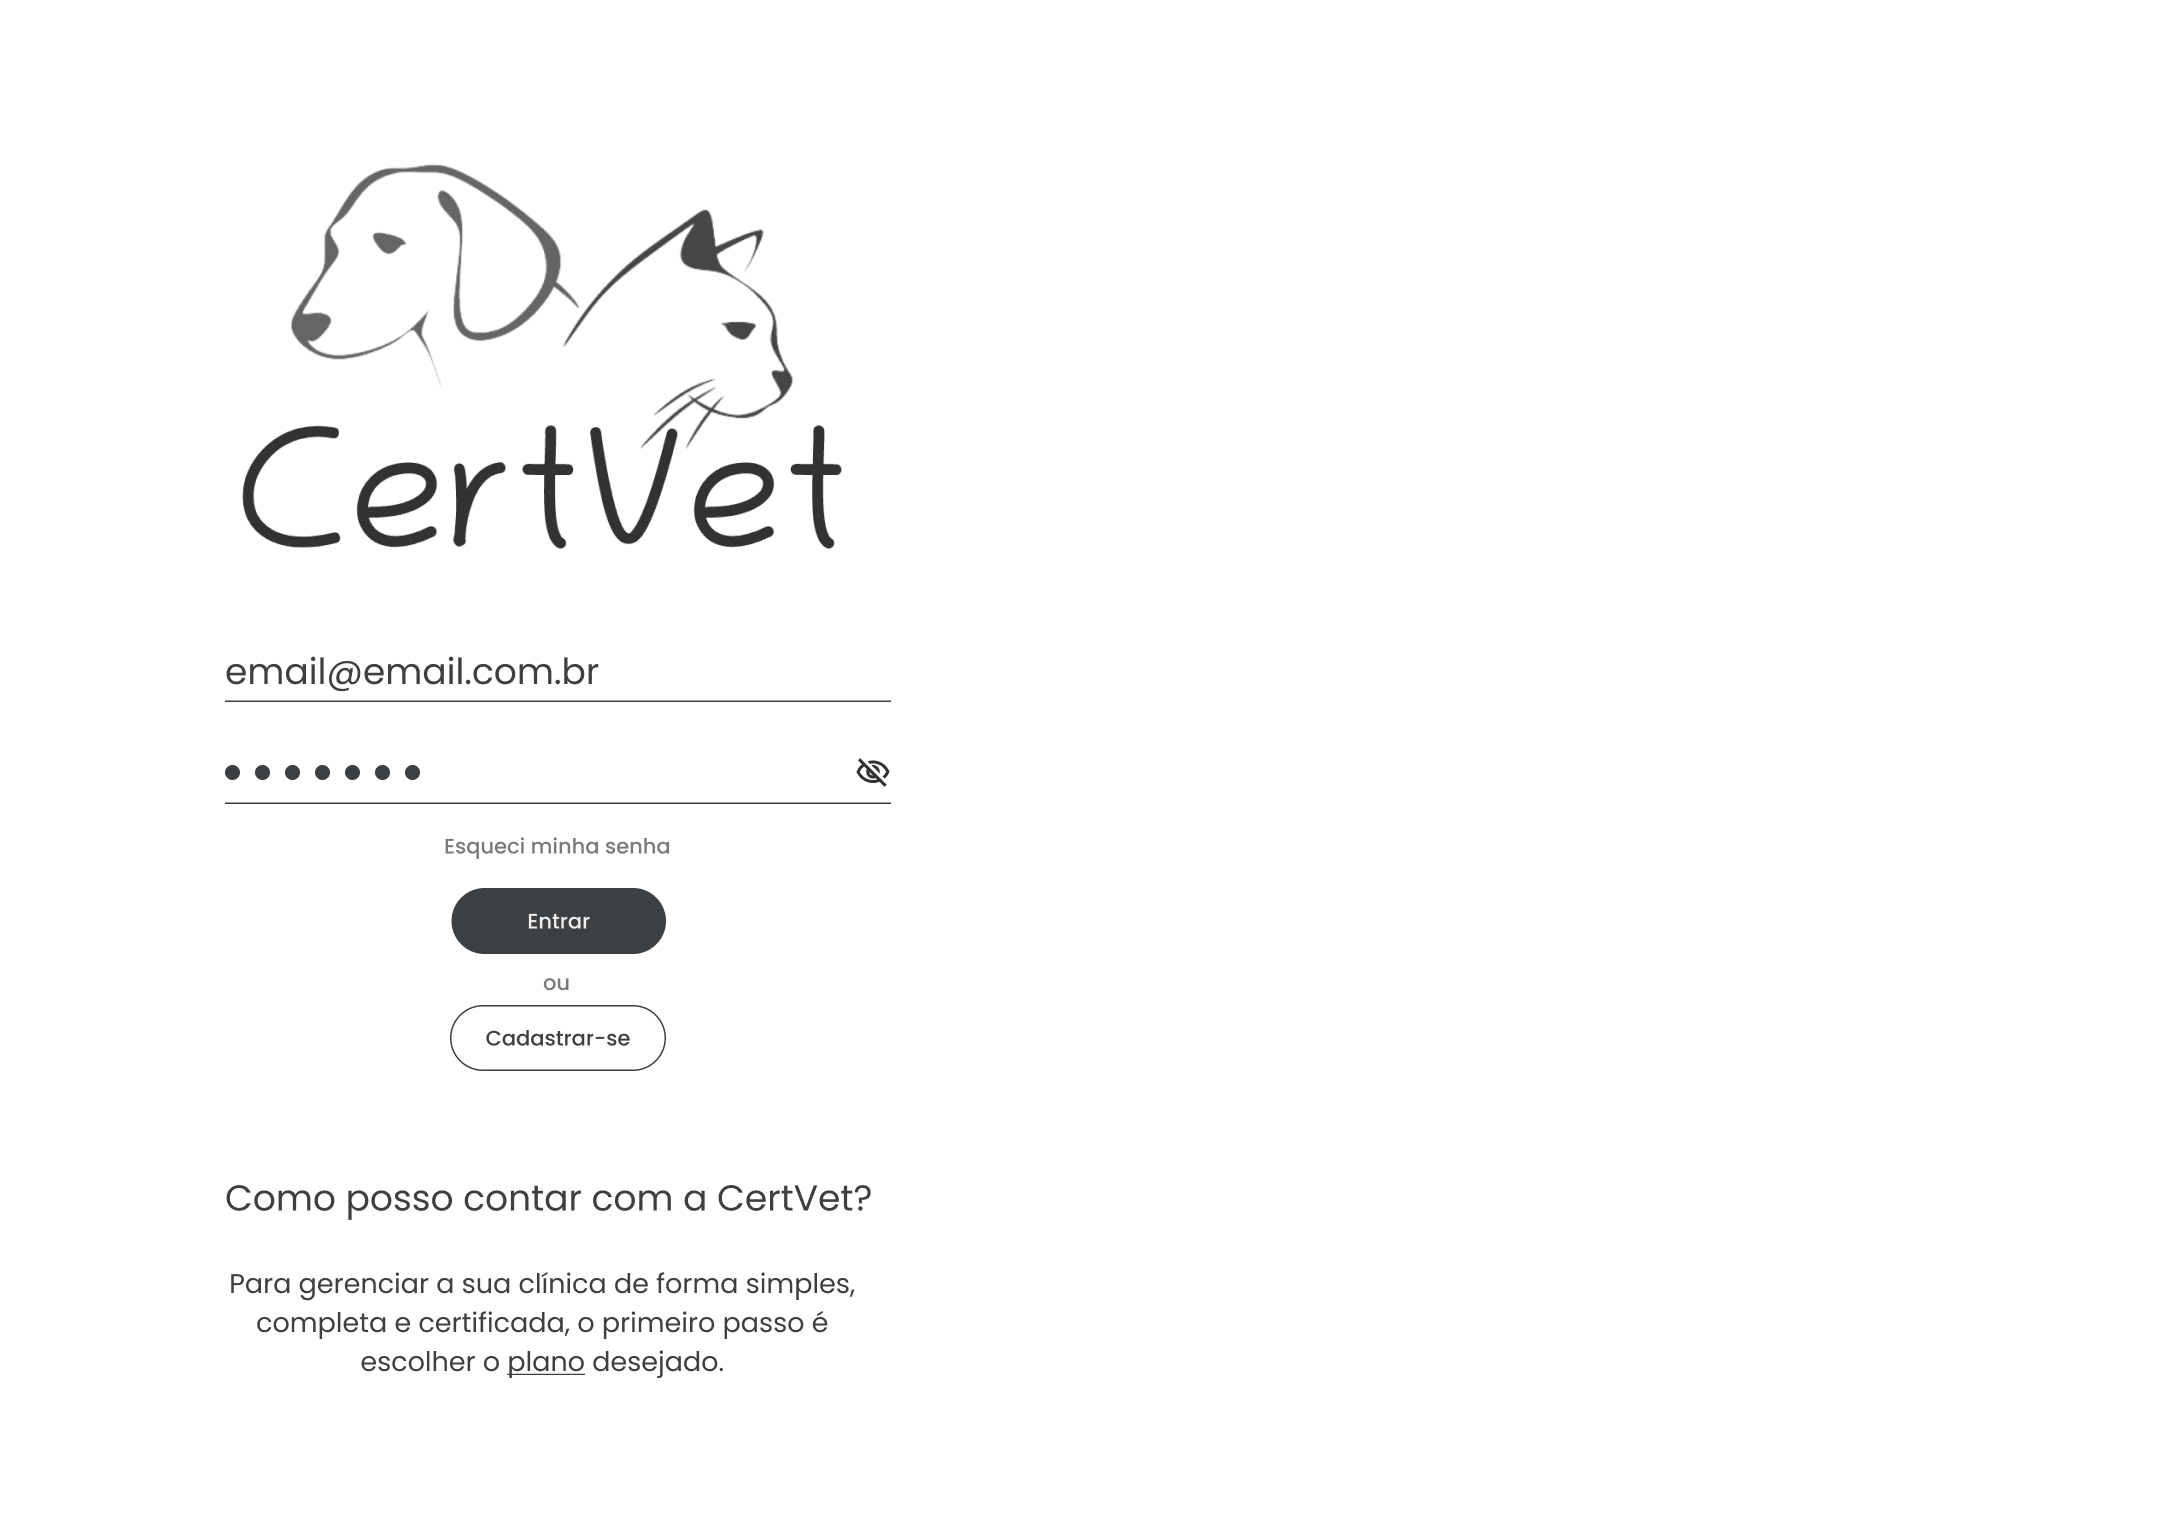
\includegraphics[width=0.7\textwidth]{images/Telas/cadastro.png}

                \label{fig:Acesso}
                \centering
        {\footnotesize \DIFaddFL{Fonte: Elaborado pelos autores.}}
            \end{figure}

\subsubsection{\DIFadd{Tela de Cadastro de Administrador}}

\DIFadd{Caso o usuário não seja cadastrado, e optar pelo botão "Cadastrar-se", ele será redirecionado para a página de cadastro de Administrador. Esse usuário poderá então cadastrar os dados do estabelecimento, assim como de outros funcionários. Este usuário pode ou não ser um médico veterinário, e para simplificar o cadastro, caso ele opte pelo sim, no campo "Veterinário", o campo CRMV se torna de preenchimento obrigatório. Fig.: \ref{fig:CadAdmin}
}

\begin{figure}[H]
                \centering
                \caption{\DIFaddFL{Tela de Cadastro de Administrador.}}
                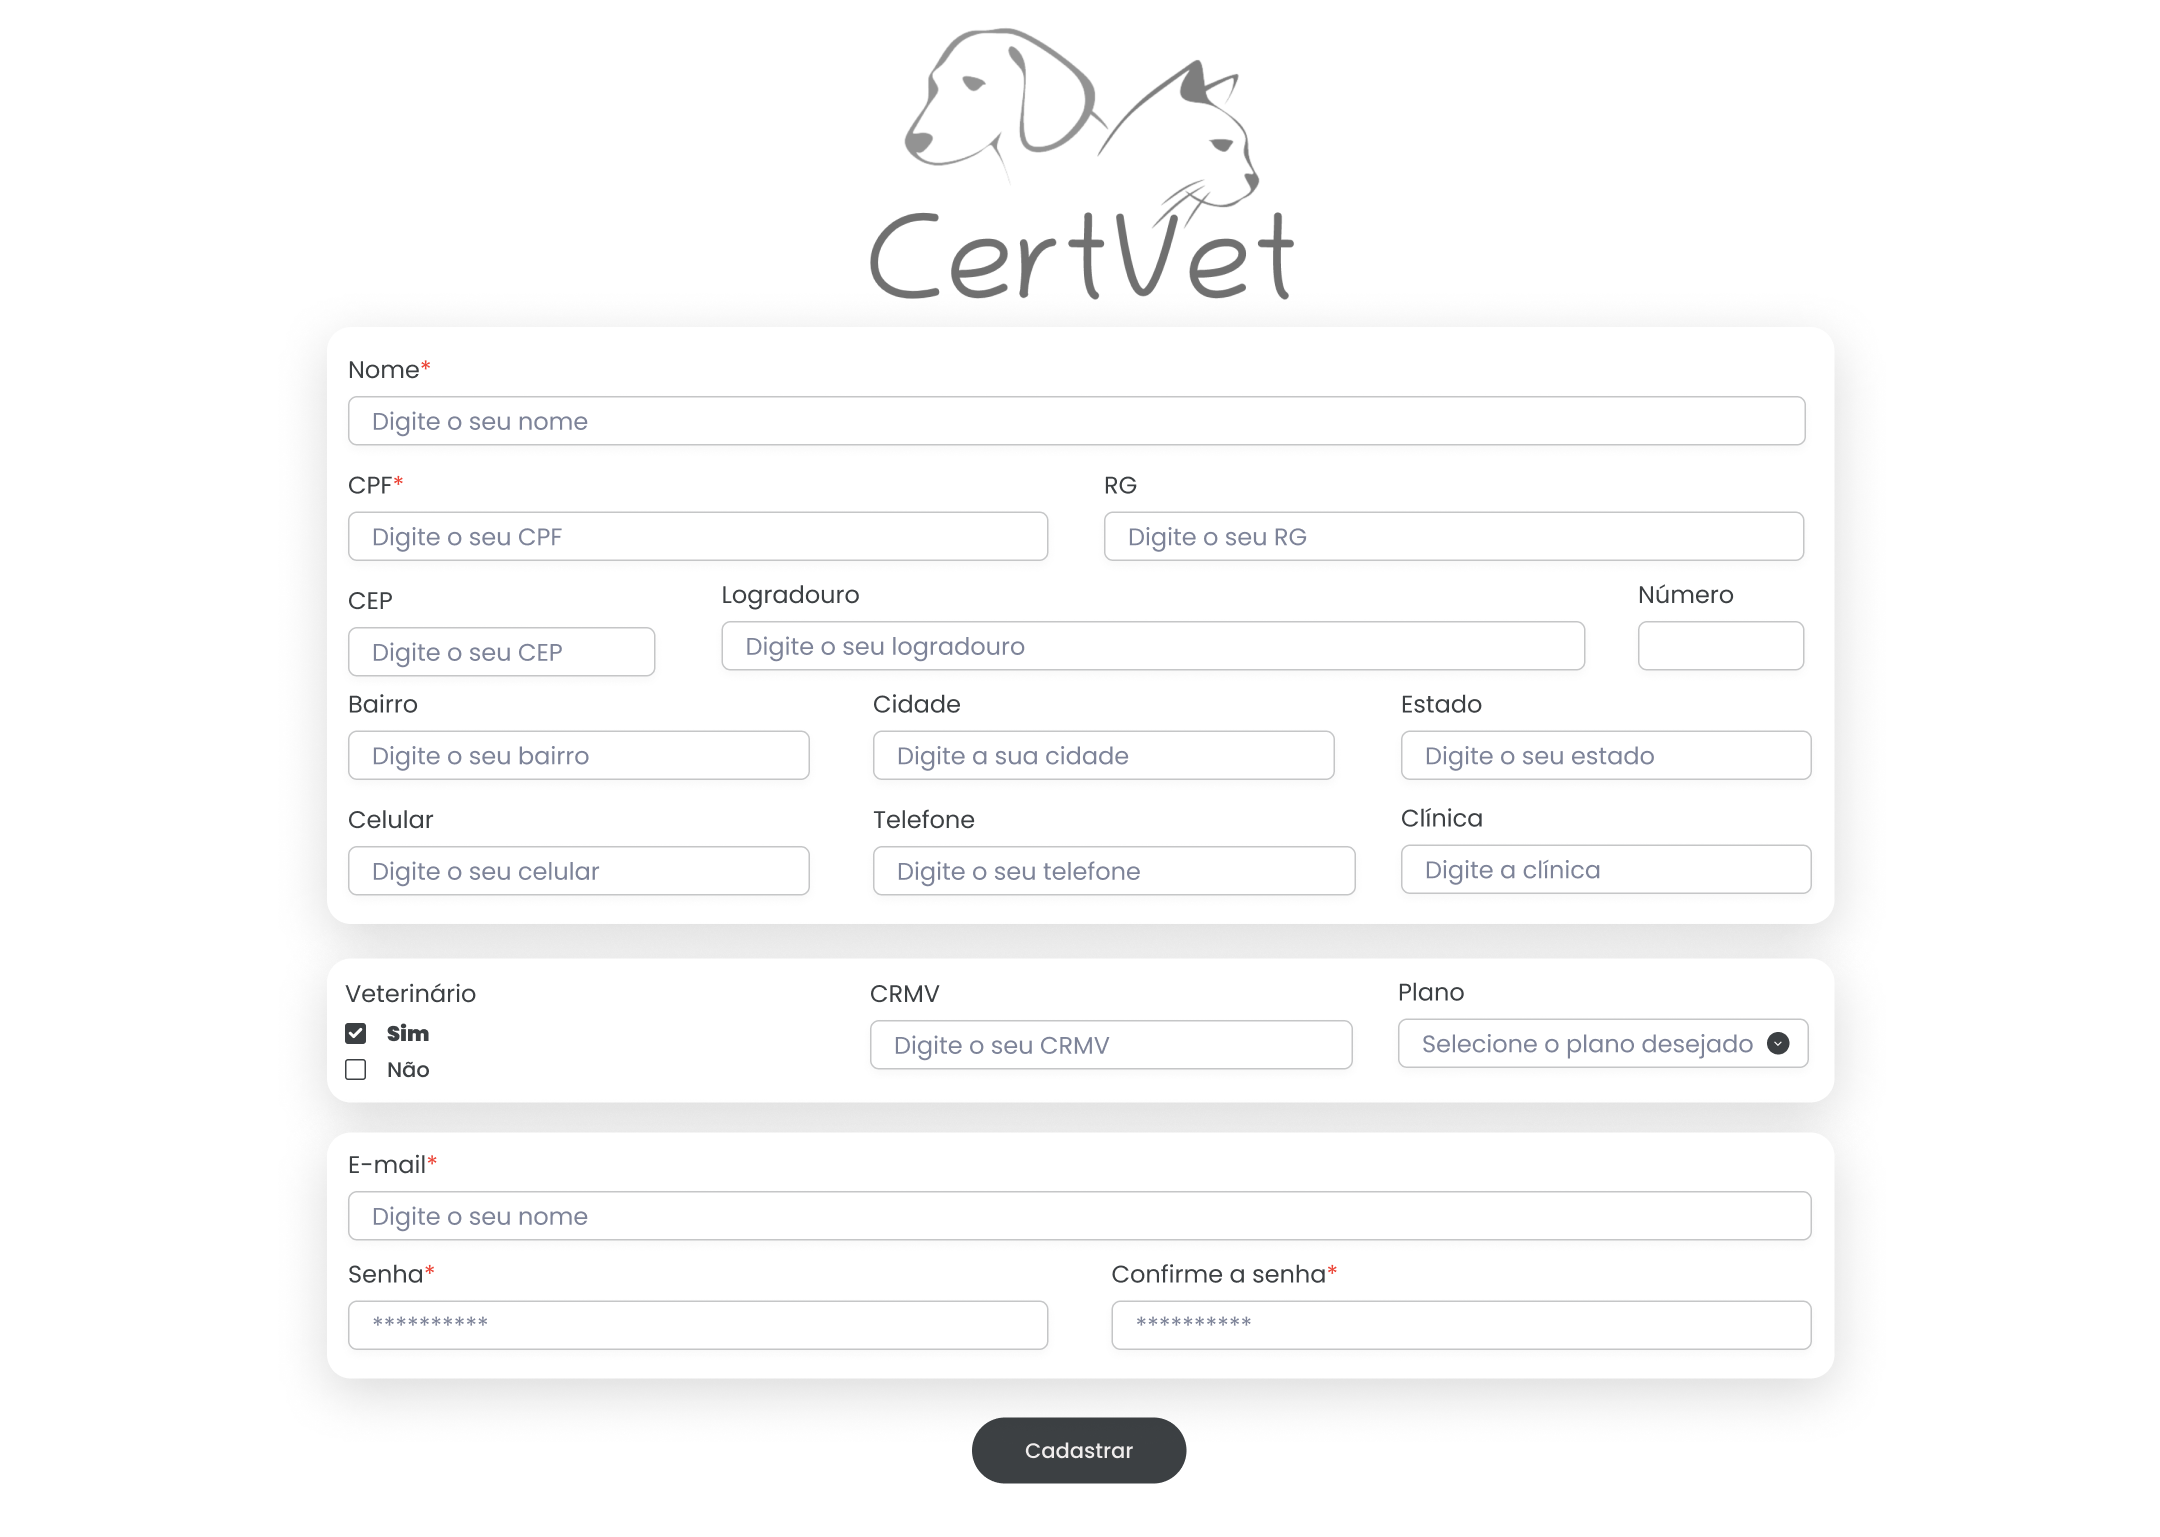
\includegraphics[width=0.7\textwidth]{images/Telas/Pagina cadastro - ADMIN.png}

                \label{fig:CadAdmin}
                \centering
        {\footnotesize \DIFaddFL{Fonte: Elaborado pelos autores.}}
            \end{figure}




\subsubsection{\DIFadd{Tela de Cadastro de Veterinário}}
\DIFadd{Quando o usuário Administrador efetuar o cadastro de outro funcionário, ele poderá enviar o }\emph{\DIFadd{login}} \DIFadd{de acesso ao funcionário, e este poderá finalizar o cadastro de seus dados no sistema. Fig.:\ref{fig:CadVet}.  
}

            \begin{figure}[H]
                \centering
                \caption{\DIFaddFL{Tela de Cadastro Final de Veterinário.}}
                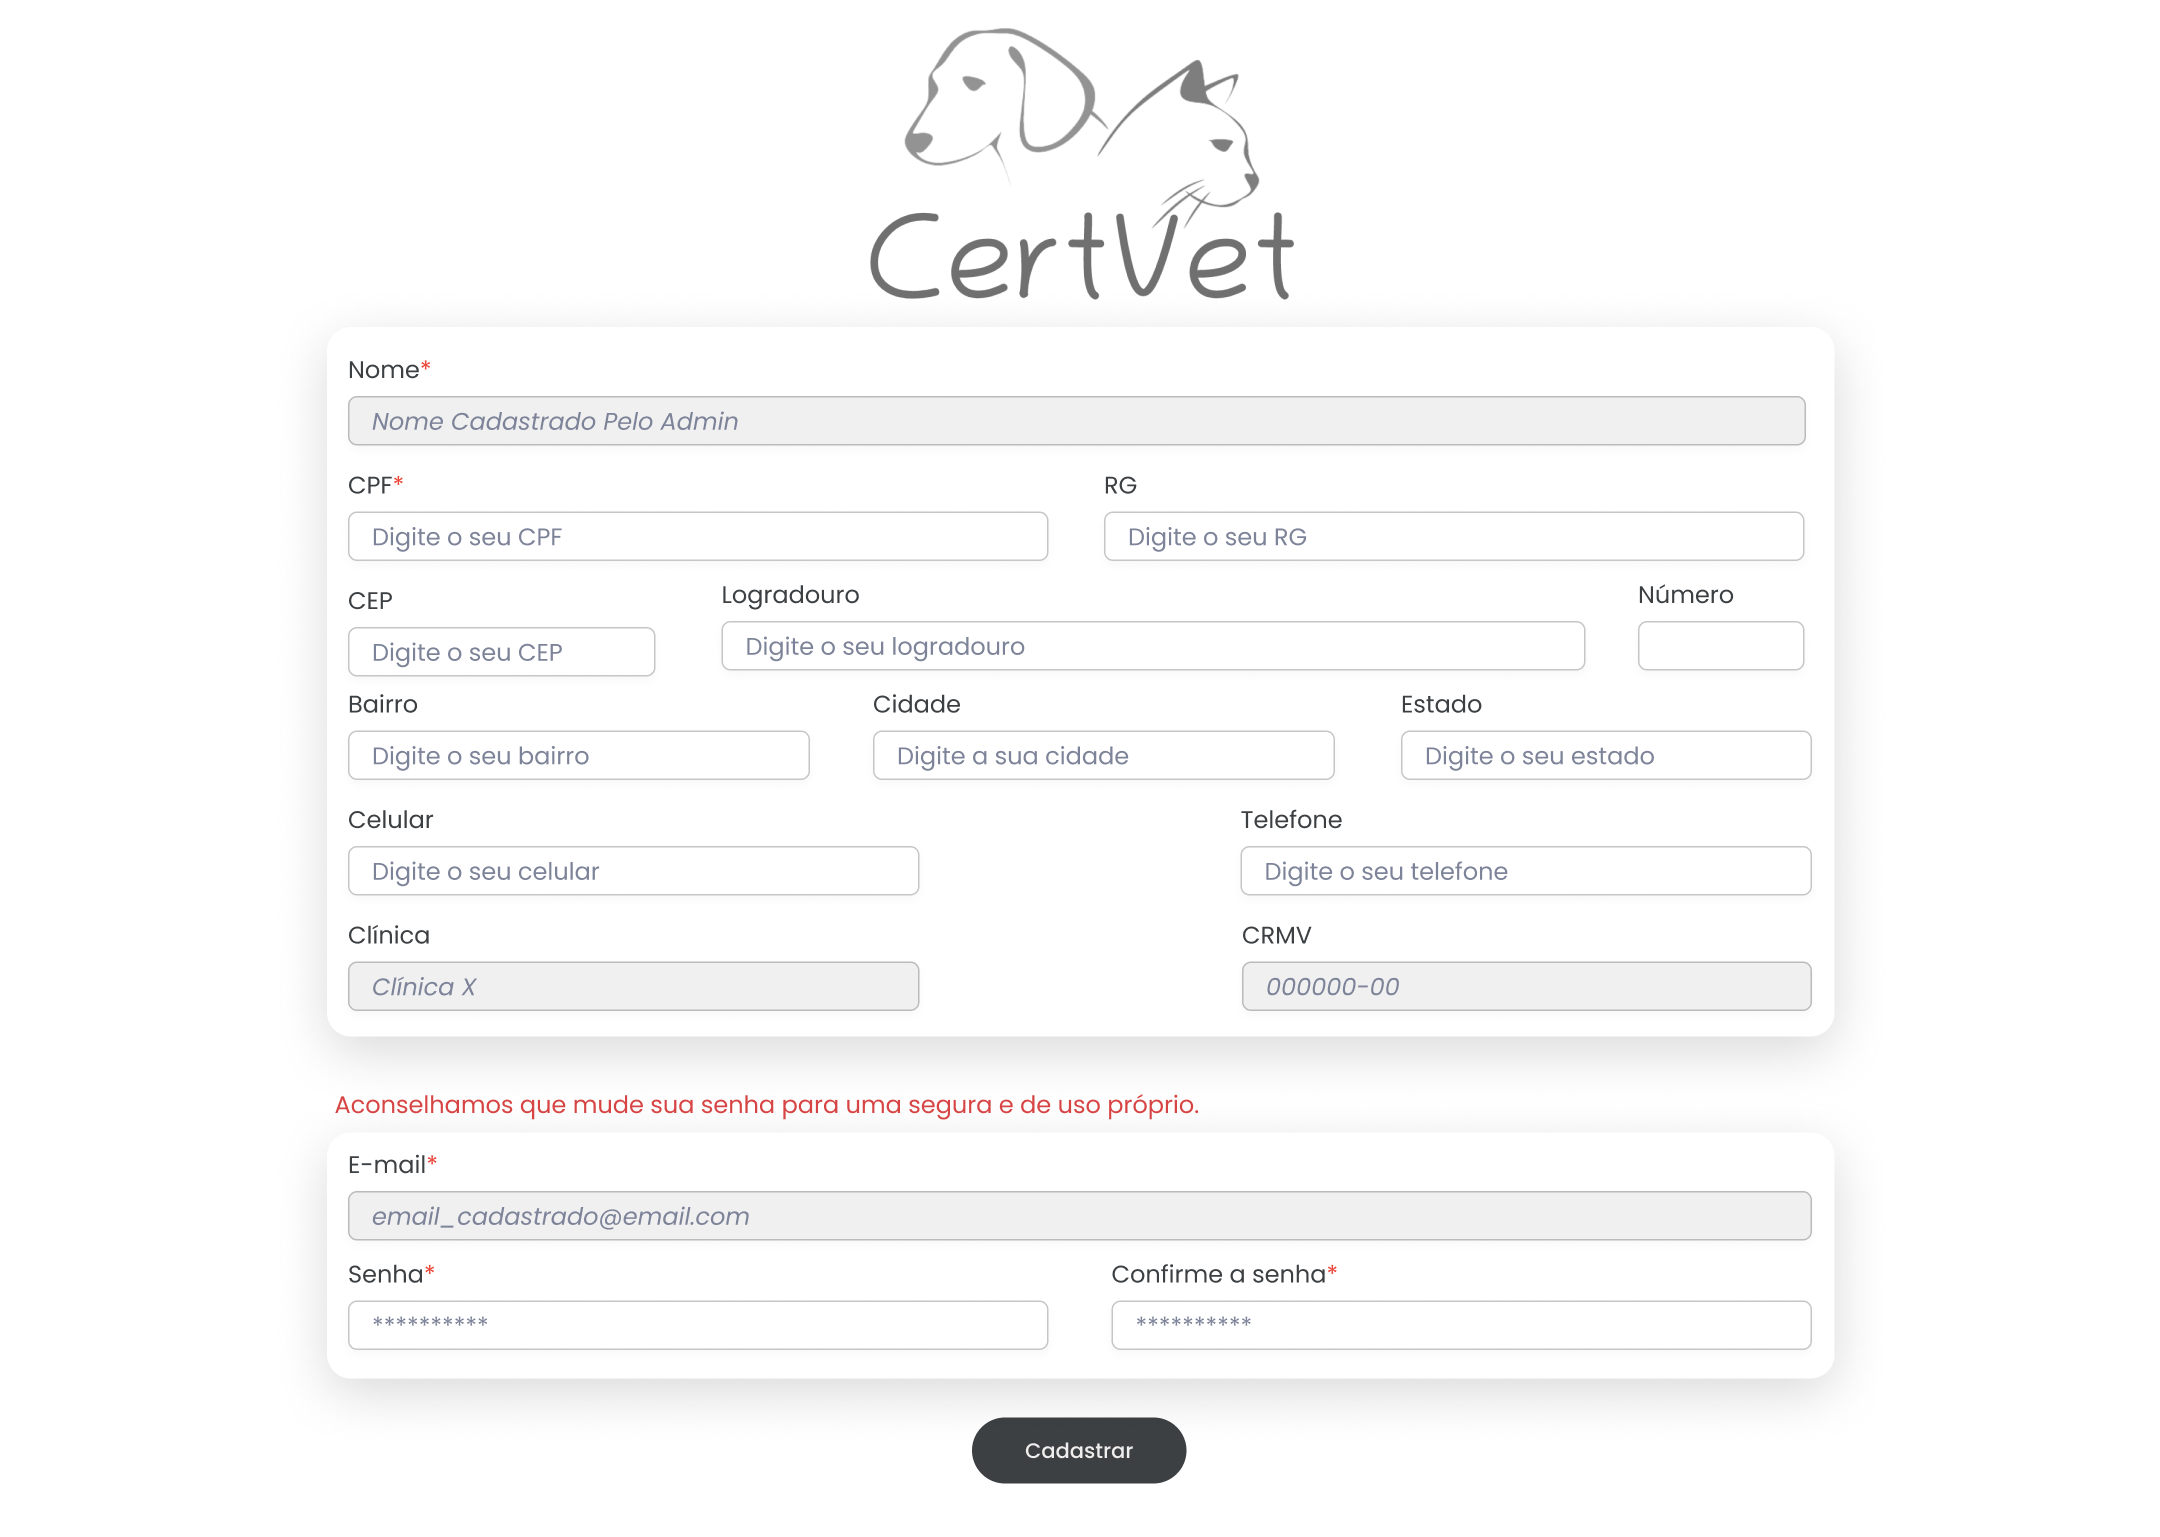
\includegraphics[width=0.7\textwidth]{images/Telas/Pagina cadastro final - VETERINARIO.png}

                \label{fig:CadVet}
                \centering
        {\footnotesize \DIFaddFL{Fonte: Elaborado pelos autores.}}
            \end{figure}


\subsubsection{\DIFadd{Tela da }\emph{\DIFadd{Dashboard}} \DIFadd{do Administrador}}

\DIFadd{Após efetuar o cadastro ou o }\emph{\DIFadd{login}}\DIFadd{, o usuário Administrador terá acessos a algumas funcionalidades básicas de gestão dos funcionários, assim como acesso as funcionalidades de veterinário, caso ele tenha confirmado seu numero de registro profissional. Fig.:\ref{fig:DashAdm}.
}

 \begin{figure}[H]
                \centering
                \caption{\DIFaddFL{Tela do }\emph{\DIFaddFL{Dashboard}} \DIFaddFL{do Administrador.}}
                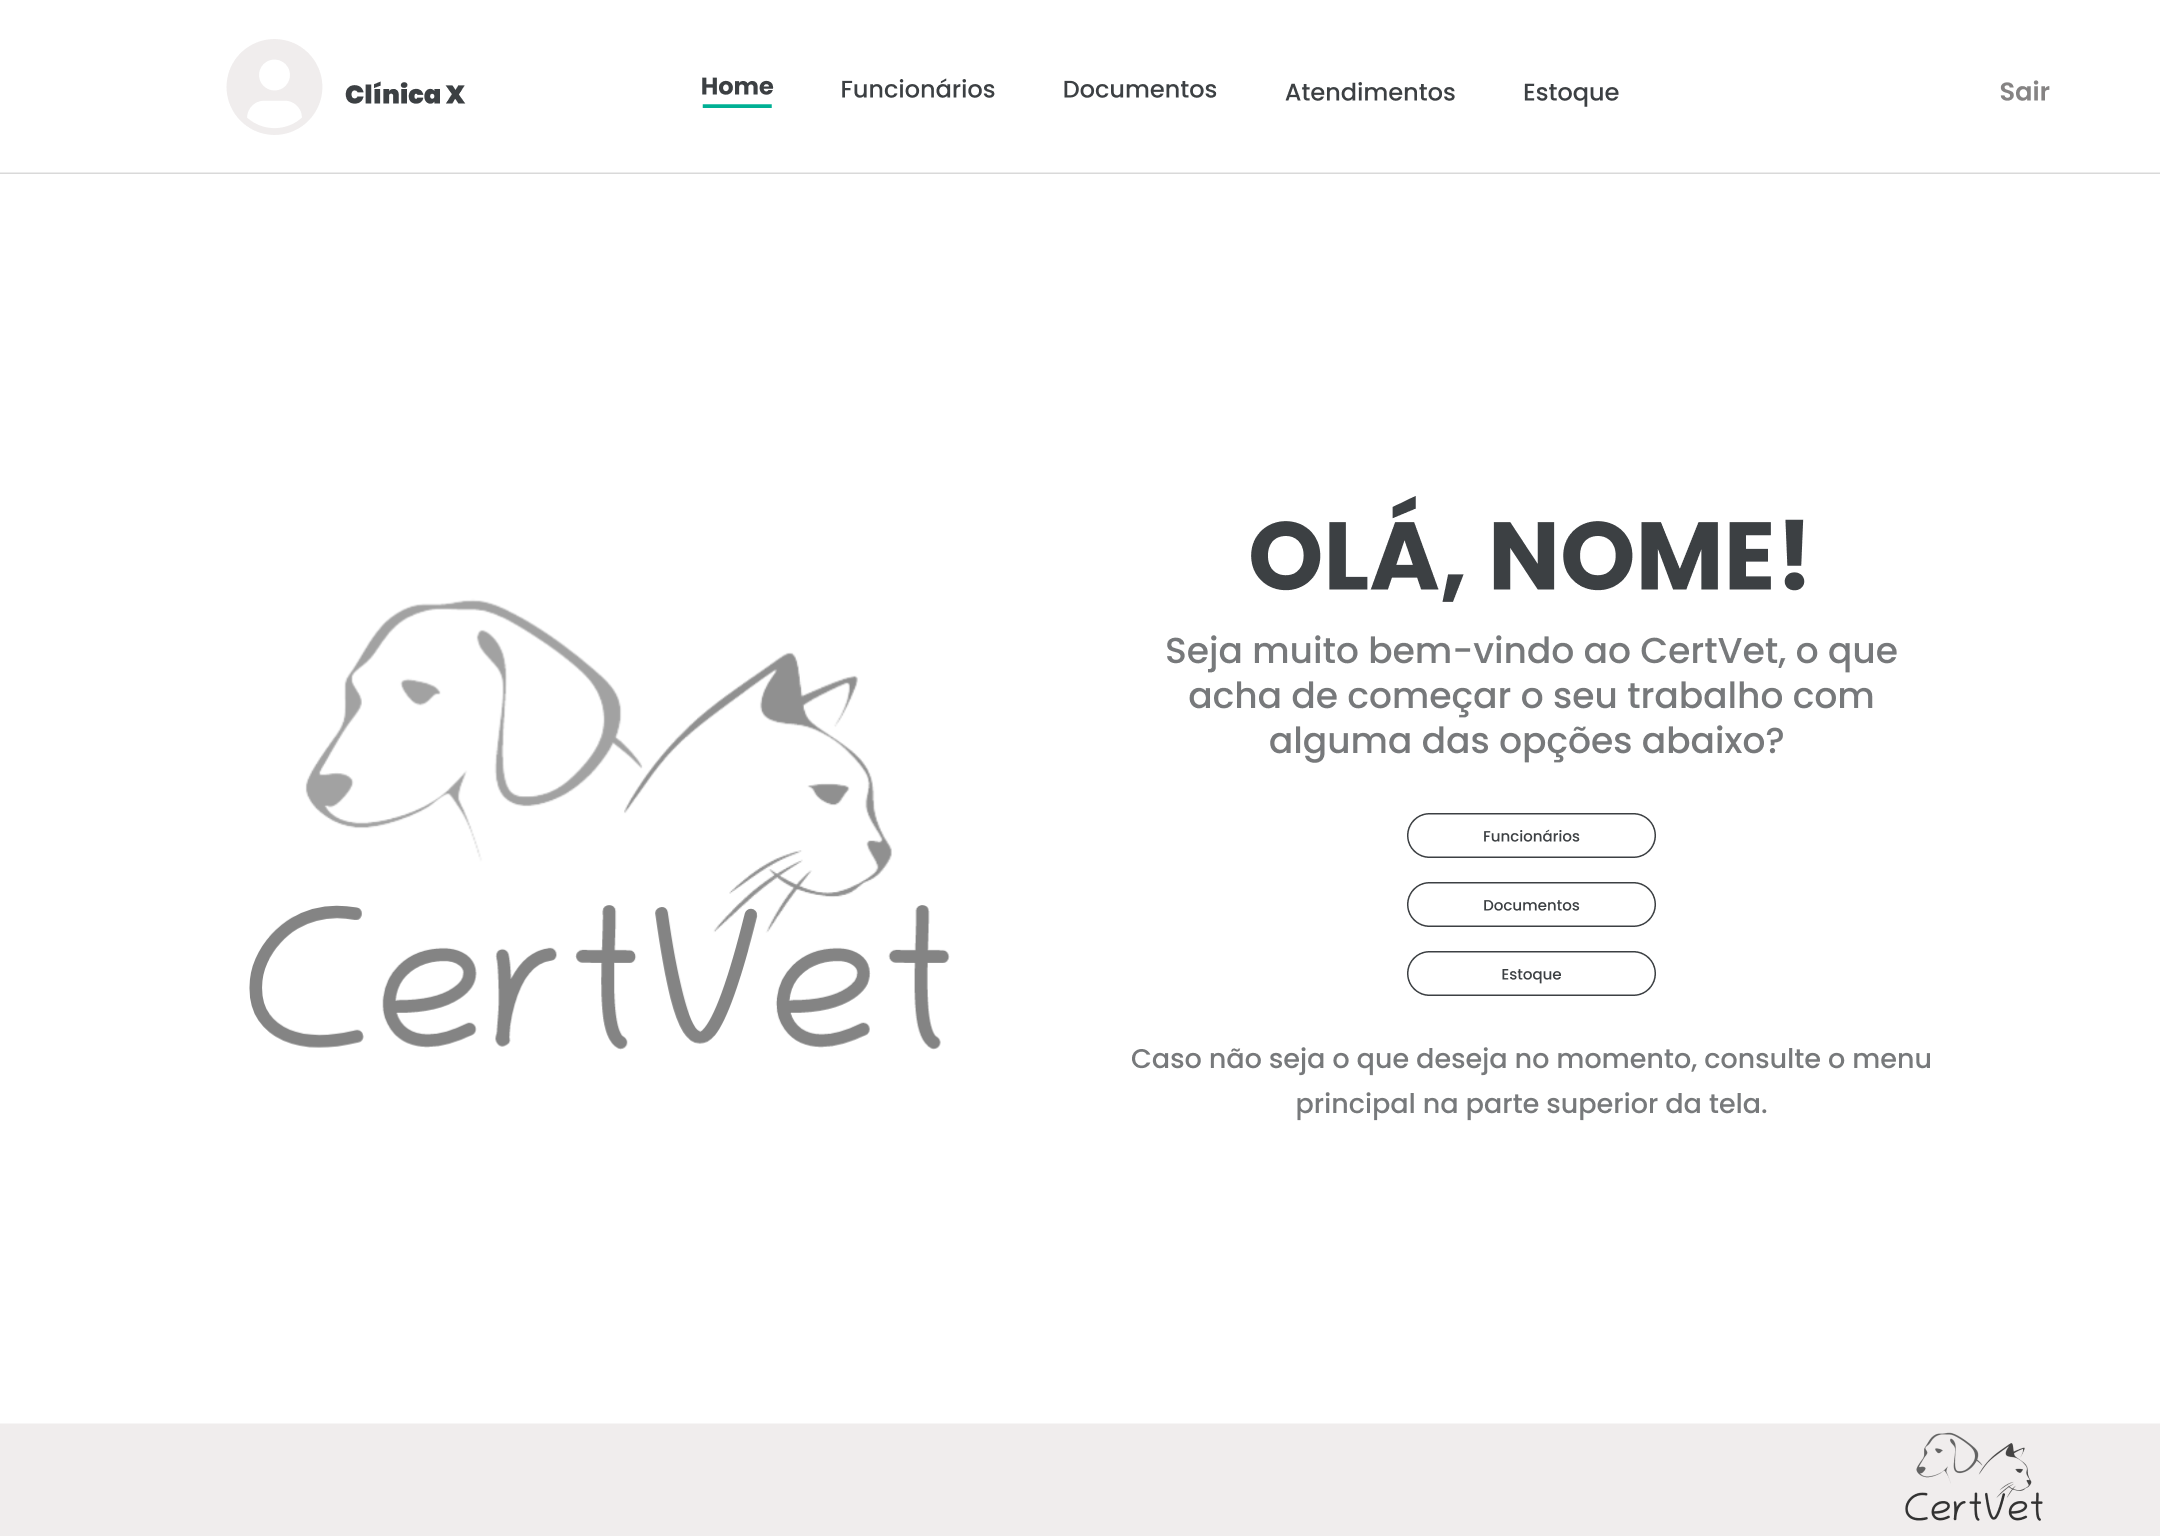
\includegraphics[width=0.7\textwidth]{images/Telas/Dashboard - ADMIN.png}

                \label{fig:DashAdm}
                \centering
        {\footnotesize \DIFaddFL{Fonte: Elaborado pelos autores.}}
            \end{figure}

    \subsubsection{\DIFadd{Tela do }\emph{\DIFadd{Dashboard}} \DIFadd{do Veterinário.}}
    \DIFadd{O usuário Veterinário, irá encontrar uma tela semelhante do Administrador, porém focado no atendimento do animal, conforme a Fig. \ref{fig:DashVet}.
    }

         \begin{figure}[H]
                \centering
                \caption{\DIFaddFL{Tela do }\emph{\DIFaddFL{Dasboard}} \DIFaddFL{do Veterinário.}}
                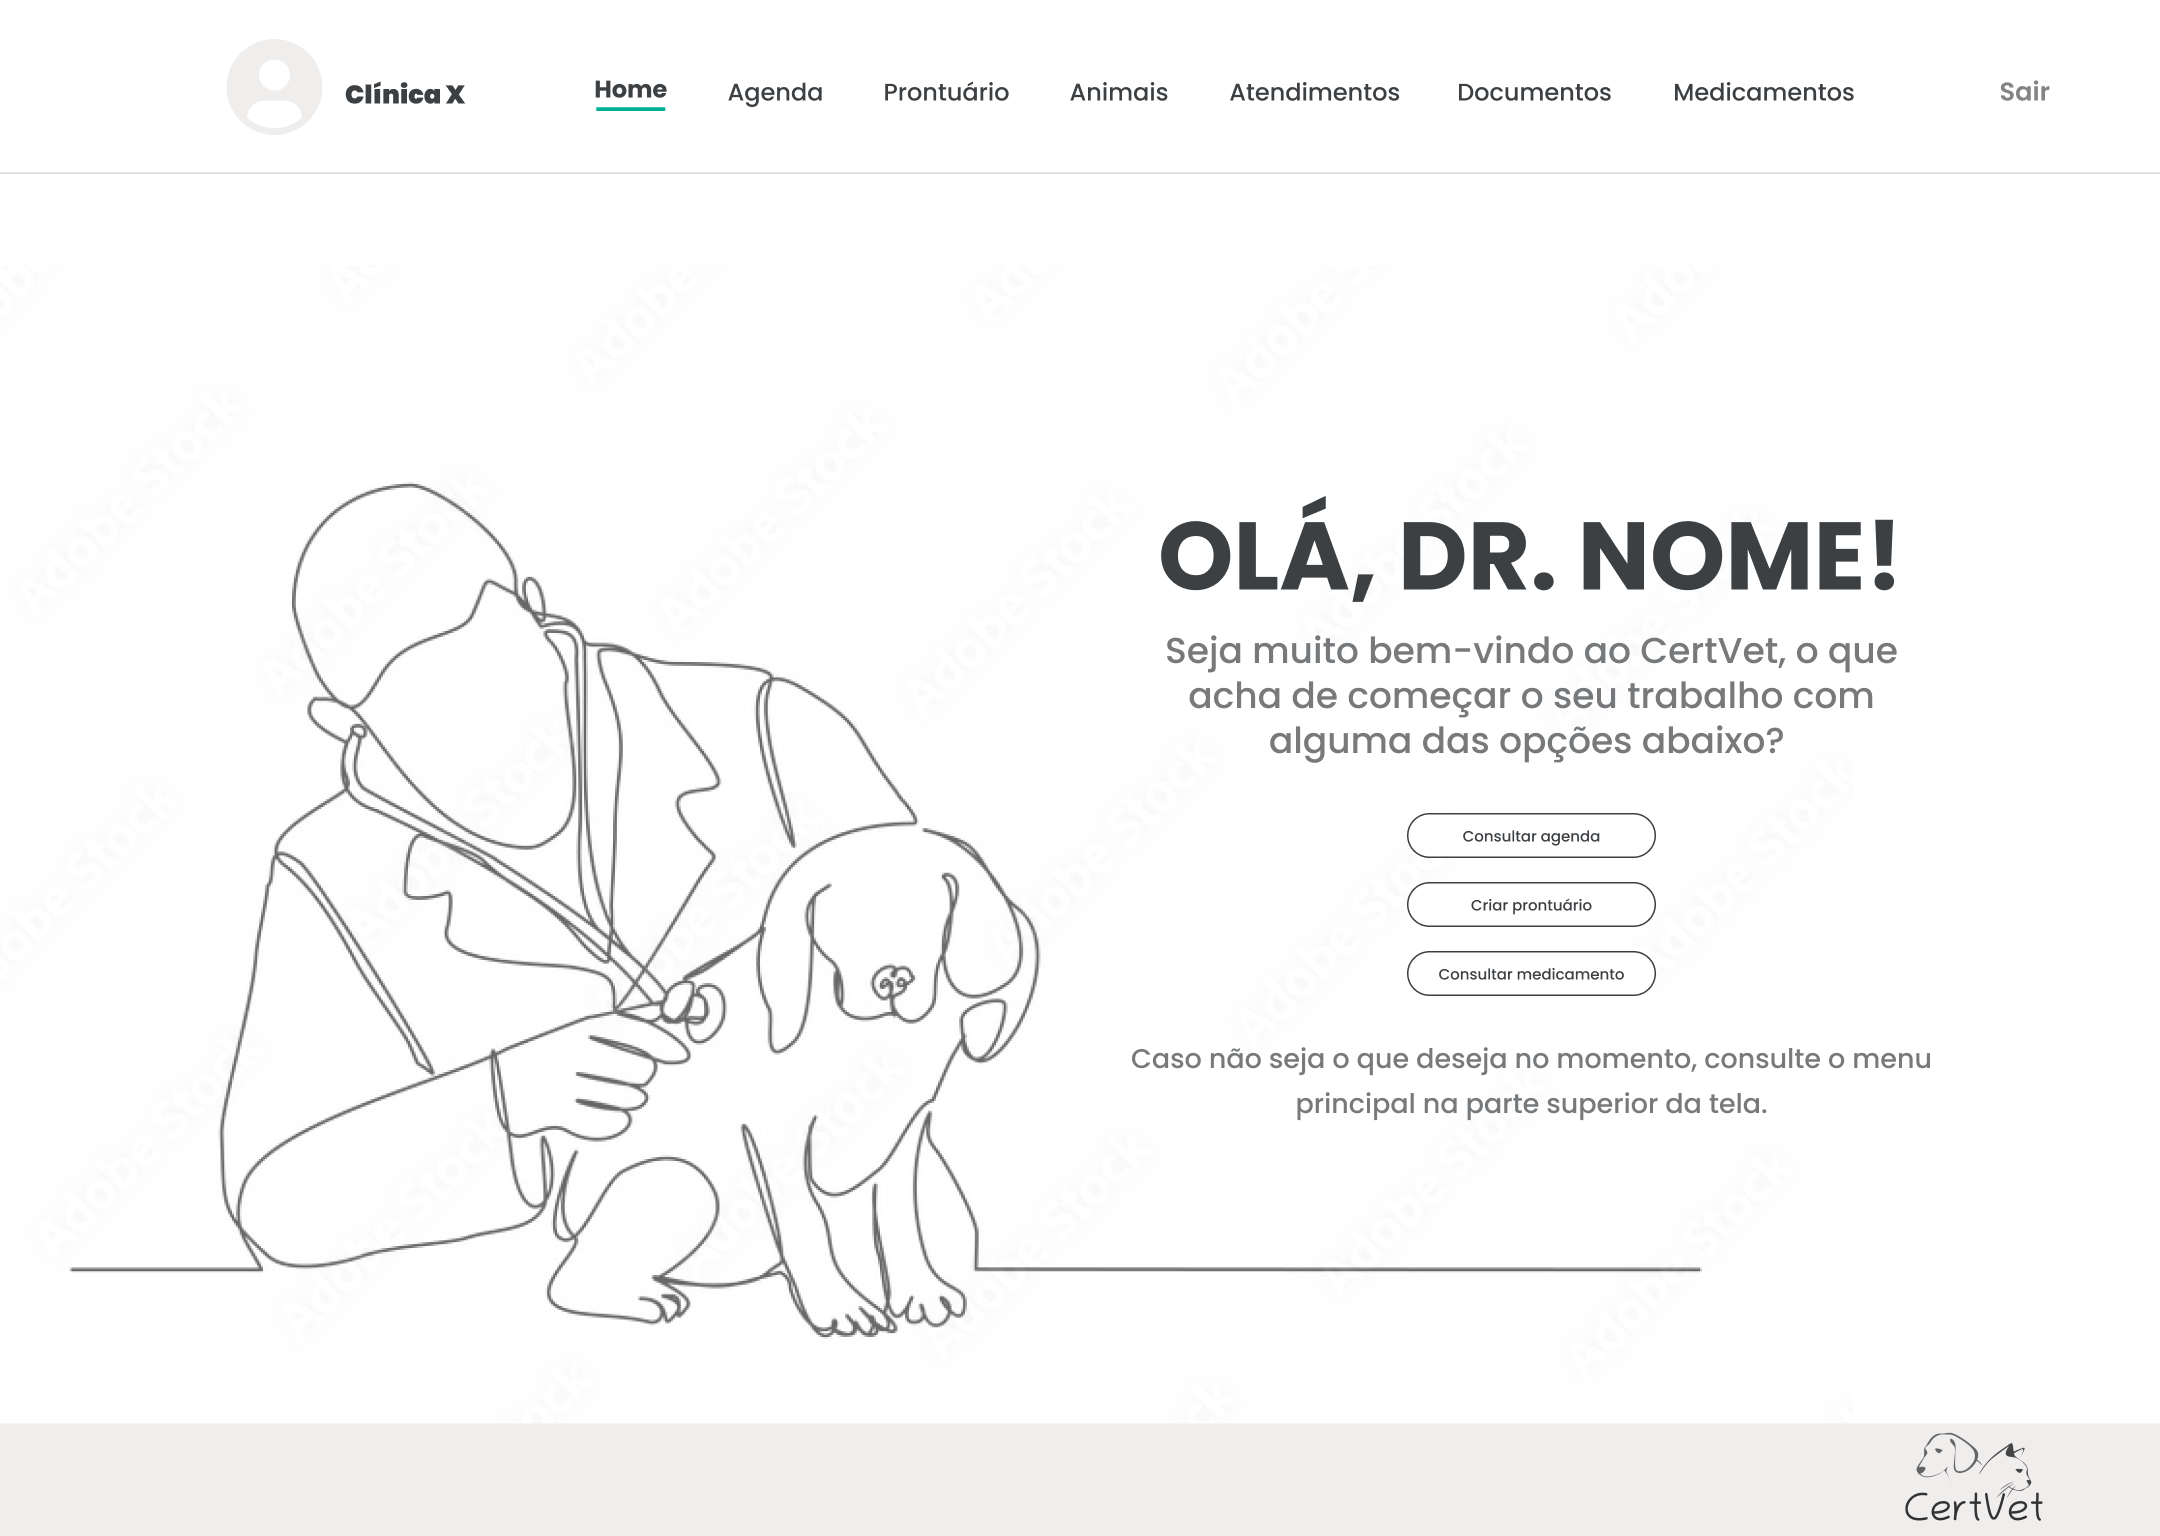
\includegraphics[width=0.7\textwidth]{images/Telas/Dashboard - VETERINARIO.png}

                \label{fig:DashVet}
                \centering
        {\footnotesize \DIFaddFL{Fonte: Elaborado pelos autores.}}
            \end{figure}    

    \subsection{\DIFadd{Telas de Cadastros e Agendamentos}}

\DIFadd{As telas referentes ao cadastro de Tutores e de Animais, assim como as de Agendamento foram feitas em baixa fidelidade, porém elas contém os dados necessários para efetuar o cadastro de forma simplificada no início, com dados básicos, podendo ser solicitado novas informações, caso seja necessário.
}

\subsubsection{\DIFadd{Tela de Cadastro de Tutor}}
\DIFadd{Para efetuar o cadastro inicial de um tutor, serão solicitados dados básicos, mas de caratér obrigatório. Dados complementares podem ser solicitados após ou durante o atendimento, de forma a agilizar o atendimento ao animal. Fig.:\ref{fig:CadTutor}.
}

\begin{figure}[H]
                \centering
                \caption{\DIFaddFL{Tela de Cadastro de Tutor.}}
                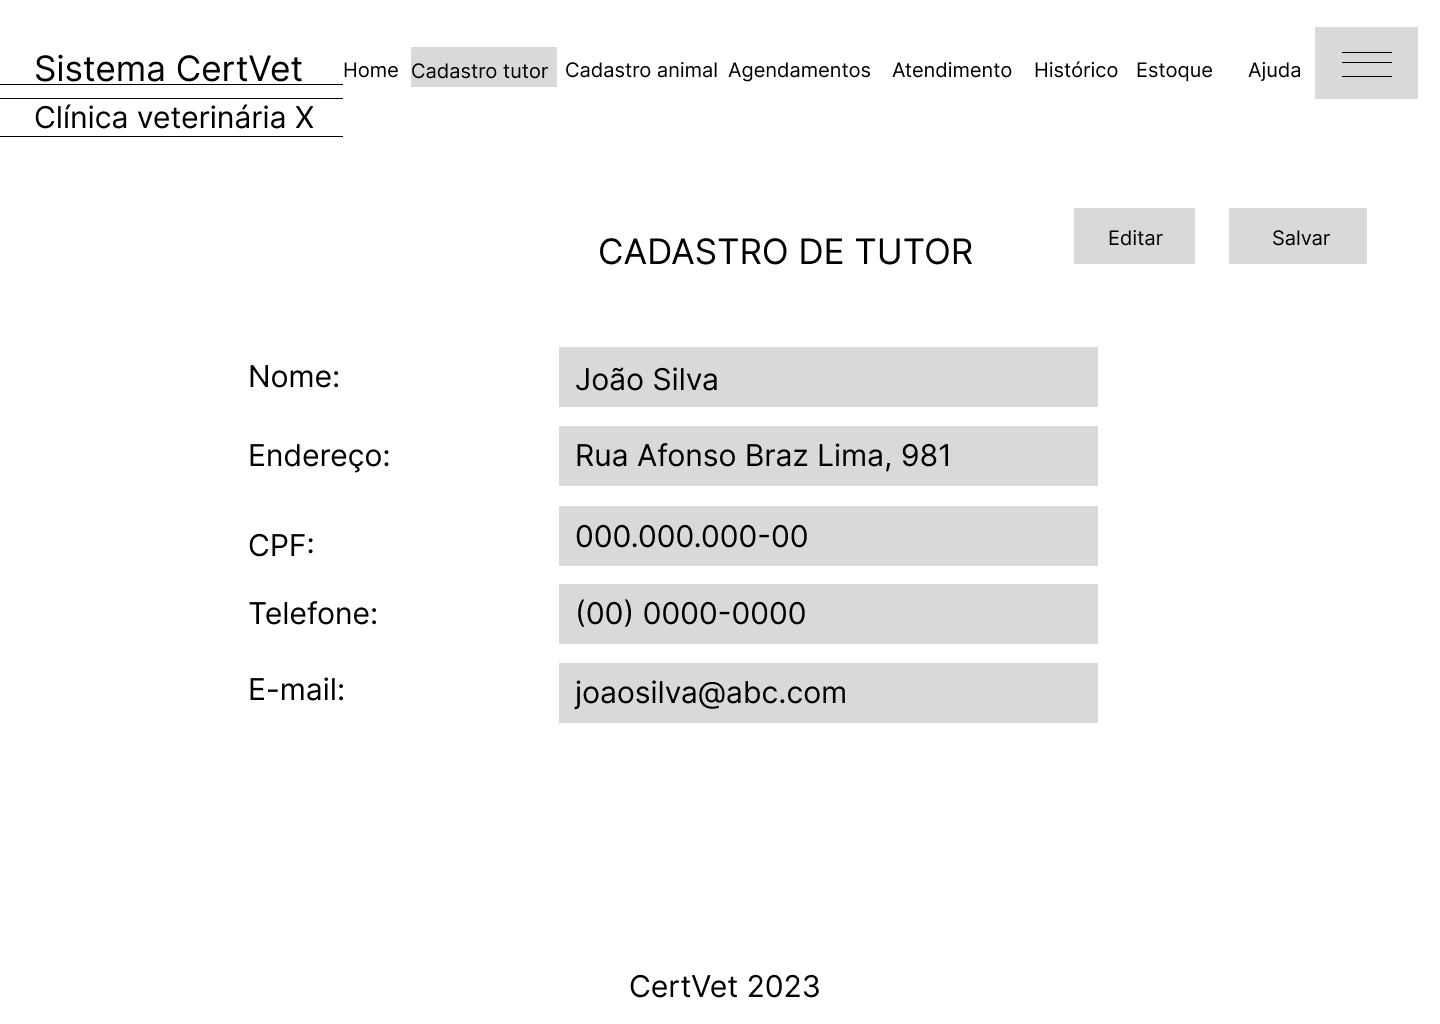
\includegraphics[width=0.7\textwidth]{images/Telas/Cadastro Tutor.png}

                \label{fig:CadTutor}
                \centering
        {\footnotesize \DIFaddFL{Fonte: Elaborado pelos autores.}}
            \end{figure}    


\subsubsection{\DIFadd{Tela de Cadastro de Animal}}
\DIFadd{Assim como a tela de Tutor, a tela de cadastro inicial do Animal coleta apenas os dados básicos do animal, podendo ser adicionada novas informações posteriormente.Fig.: \ref{fig:CadAnimal}.
}

\begin{figure}[H]
                \centering
                \caption{\DIFaddFL{Tela de Cadastro do Animal.}}
                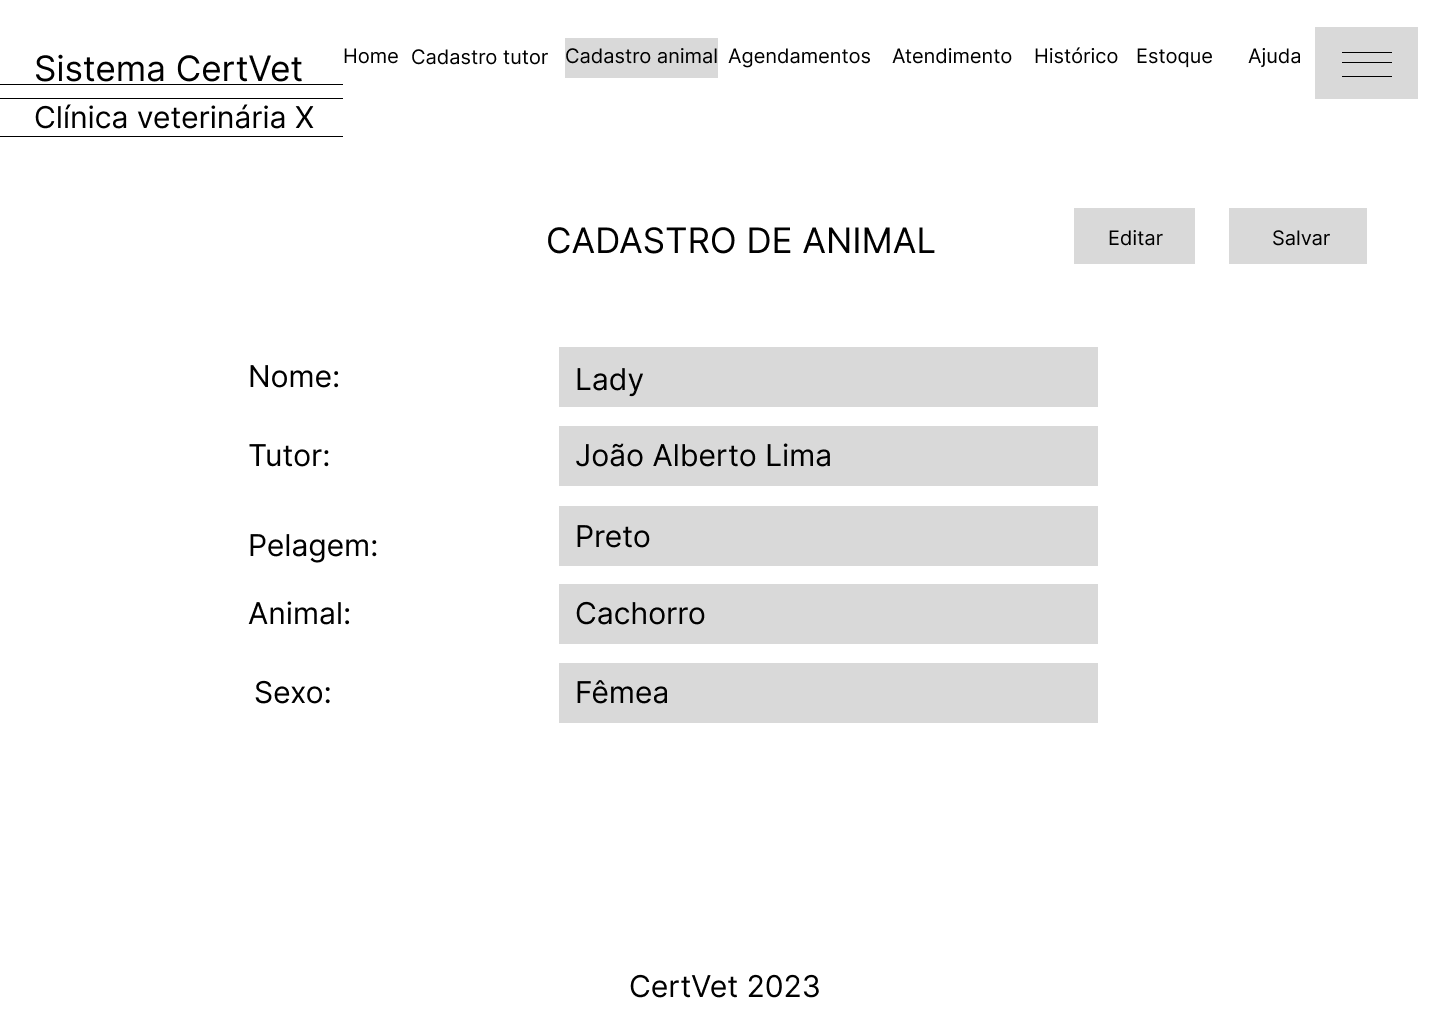
\includegraphics[width=0.7\textwidth]{images/Telas/Cadastro Animal.png}

                \label{fig:CadAnimal}
                \centering
        {\footnotesize \DIFaddFL{Fonte: Elaborado pelos autores.}}
            \end{figure}    

\subsubsection{\DIFadd{Telas de Agendamento}}

\DIFadd{As telas de Agendamento podem ser acessadas através da função Agendamento, Fig. \ref{fig:Calendario}. Após selecionar o dia, um modal será aberto, com os horarios ocupados e vagos, Fig. \ref{fig:Agenda}  um horário vago, é possível inserir dados para um novo agendamento, \ref{fig:Agenda2}
}


\begin{figure}[H]
                \centering
                \caption{\DIFaddFL{Tela de Agendamento - Visão Geral.}}
                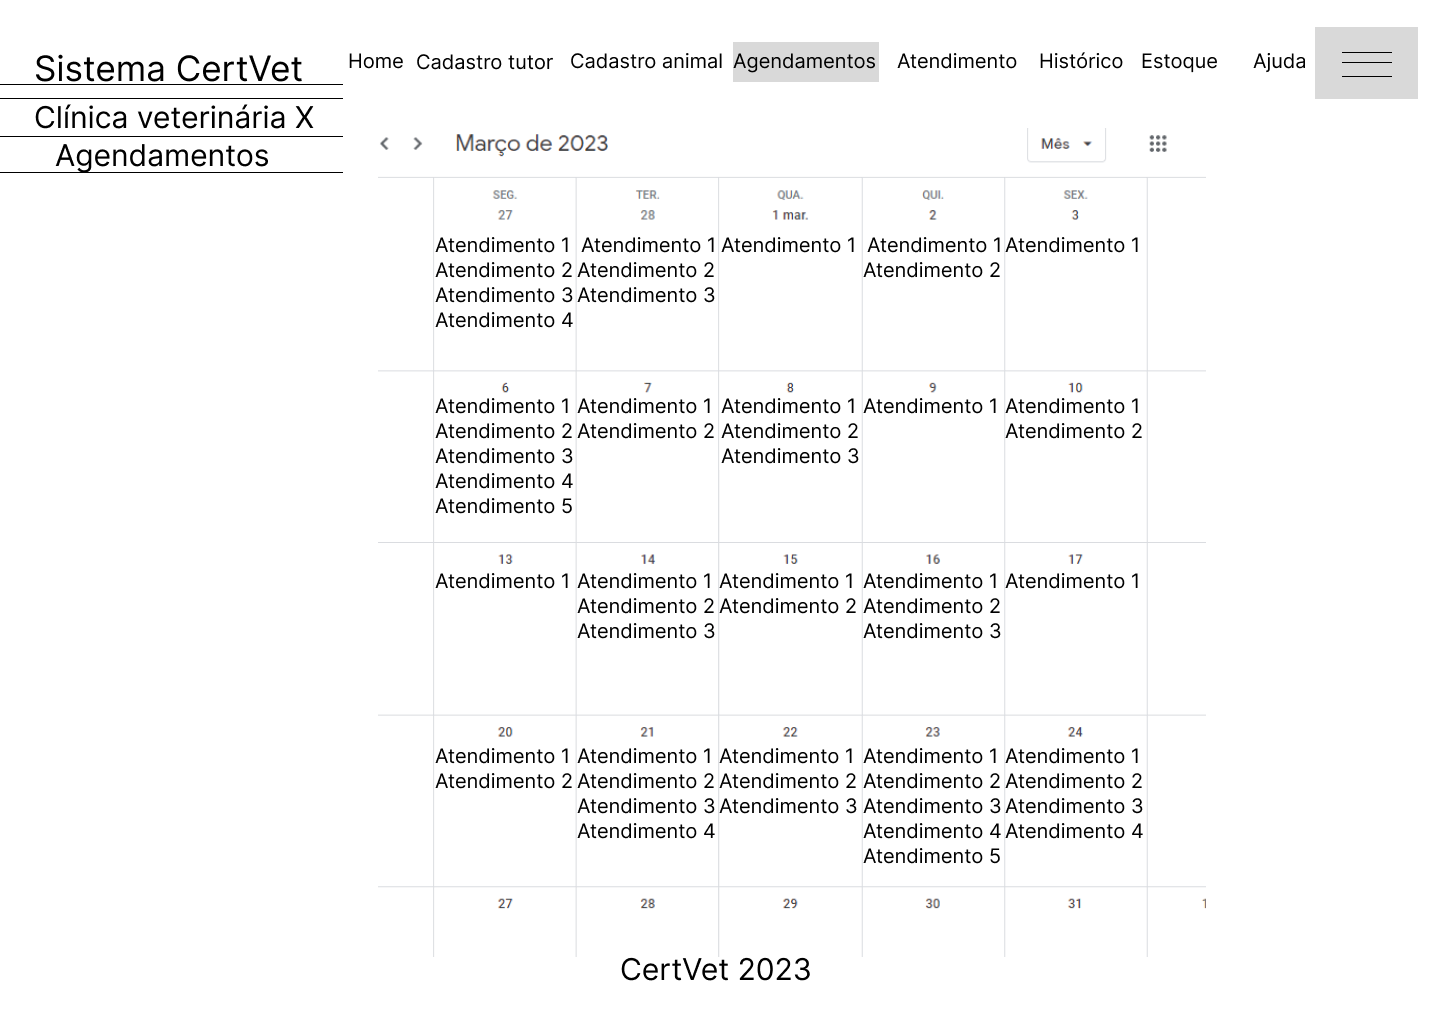
\includegraphics[width=0.7\textwidth]{images/Telas/Calendario Agenda.png}

                \label{fig:Calendario}
                \centering
        {\footnotesize \DIFaddFL{Fonte: Elaborado pelos autores.}}
            \end{figure}    

\begin{figure}[H]
                \centering
                \caption{\DIFaddFL{Tela de Agendamento - Visão Dia.}}
                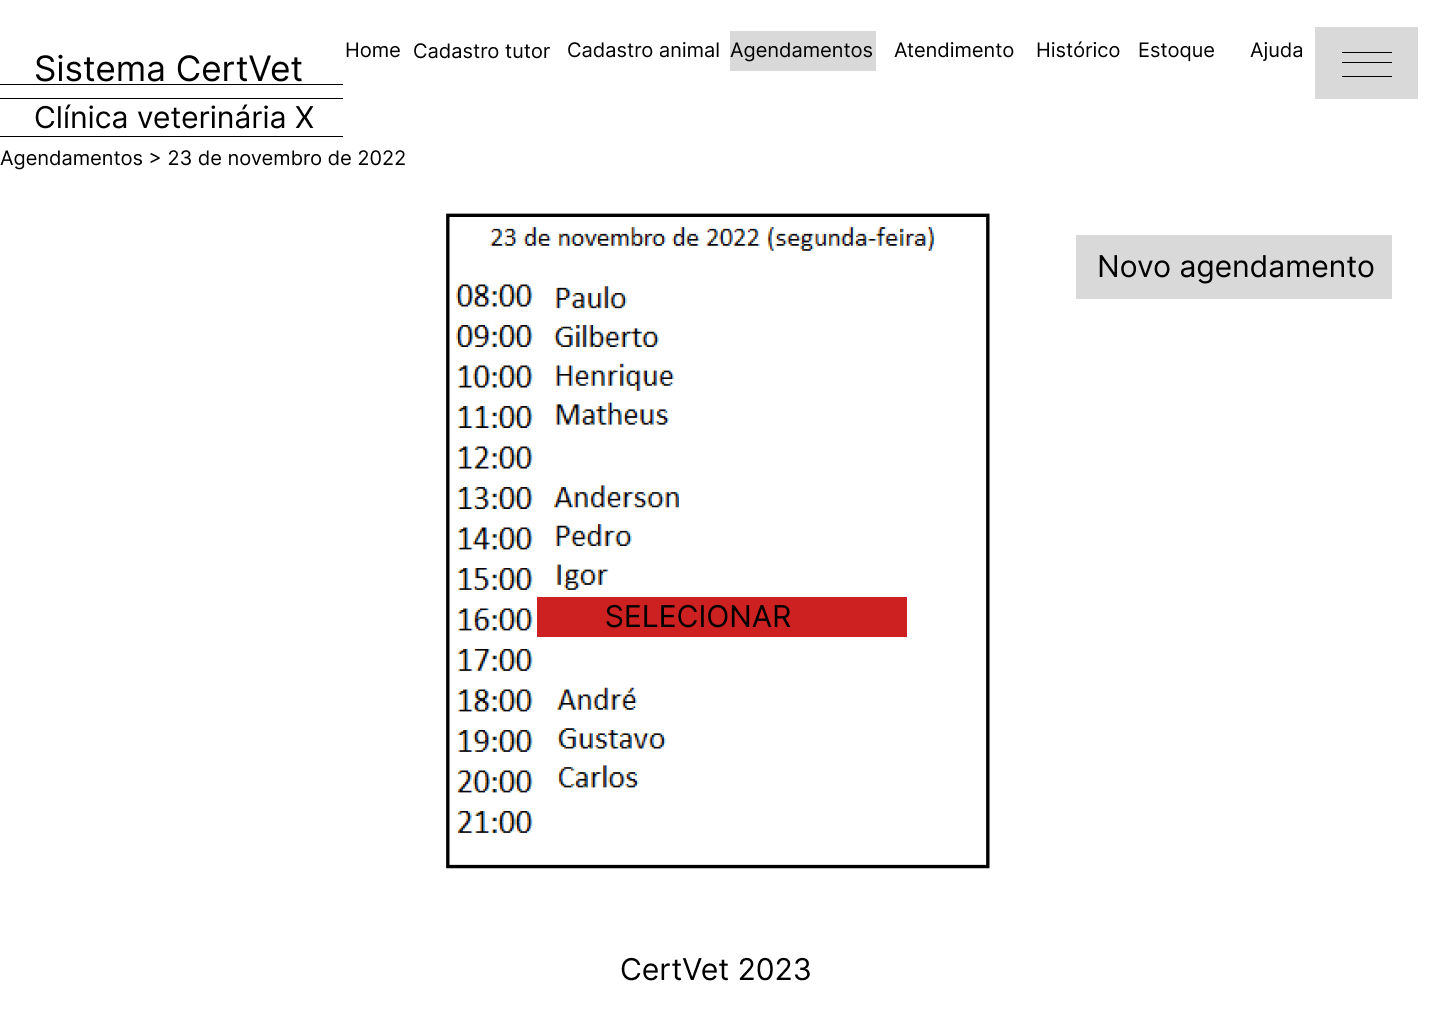
\includegraphics[width=0.7\textwidth]{images/Telas/Tela Marcar Agenda.png}

                \label{fig:Agenda}
                \centering
        {\footnotesize \DIFaddFL{Fonte: Elaborado pelos autores.}}
            \end{figure}    


\begin{figure}[H]
                \centering
                \caption{\DIFaddFL{Tela de Agendamento - Visão Cadastro.}}
                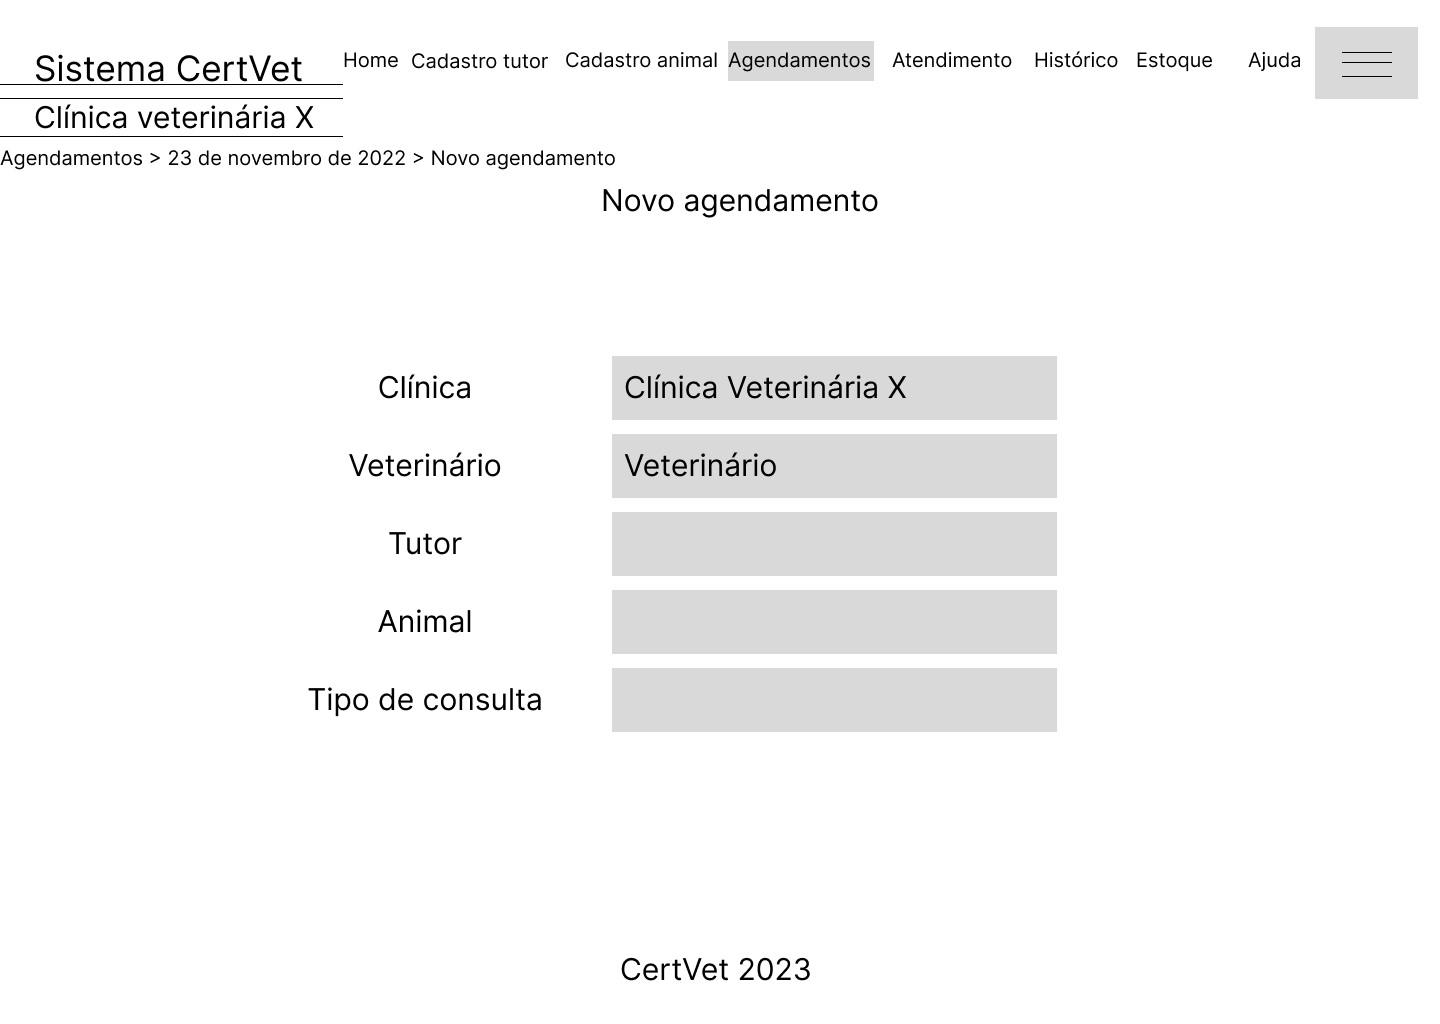
\includegraphics[width=0.7\textwidth]{images/Telas/Tela Marcar Agenda2.png}

                \label{fig:Agenda2}
                \centering
        {\footnotesize \DIFaddFL{Fonte: Elaborado pelos autores.}}
            \end{figure}    

    \subsection{\DIFadd{Telas de Atendimento Veterinário}}

\DIFadd{As telas relacionadas ao fluxo de atendimento veterinário foram planejadas de forma a serem preenchidas de forma eficiente, com campos principais em primeiro plano e também separadas por etapas durante o atendimento. Na figura \ref{fig:ProntuarioWF}, temos os campos em versão colapsada e, ao clicar nas opções, um modal deverá abrir para preenchimento dos dados. 
}

\begin{figure}[H]
                \centering
                \caption{\DIFaddFL{Tela de Elaboração de Prontuário}}
                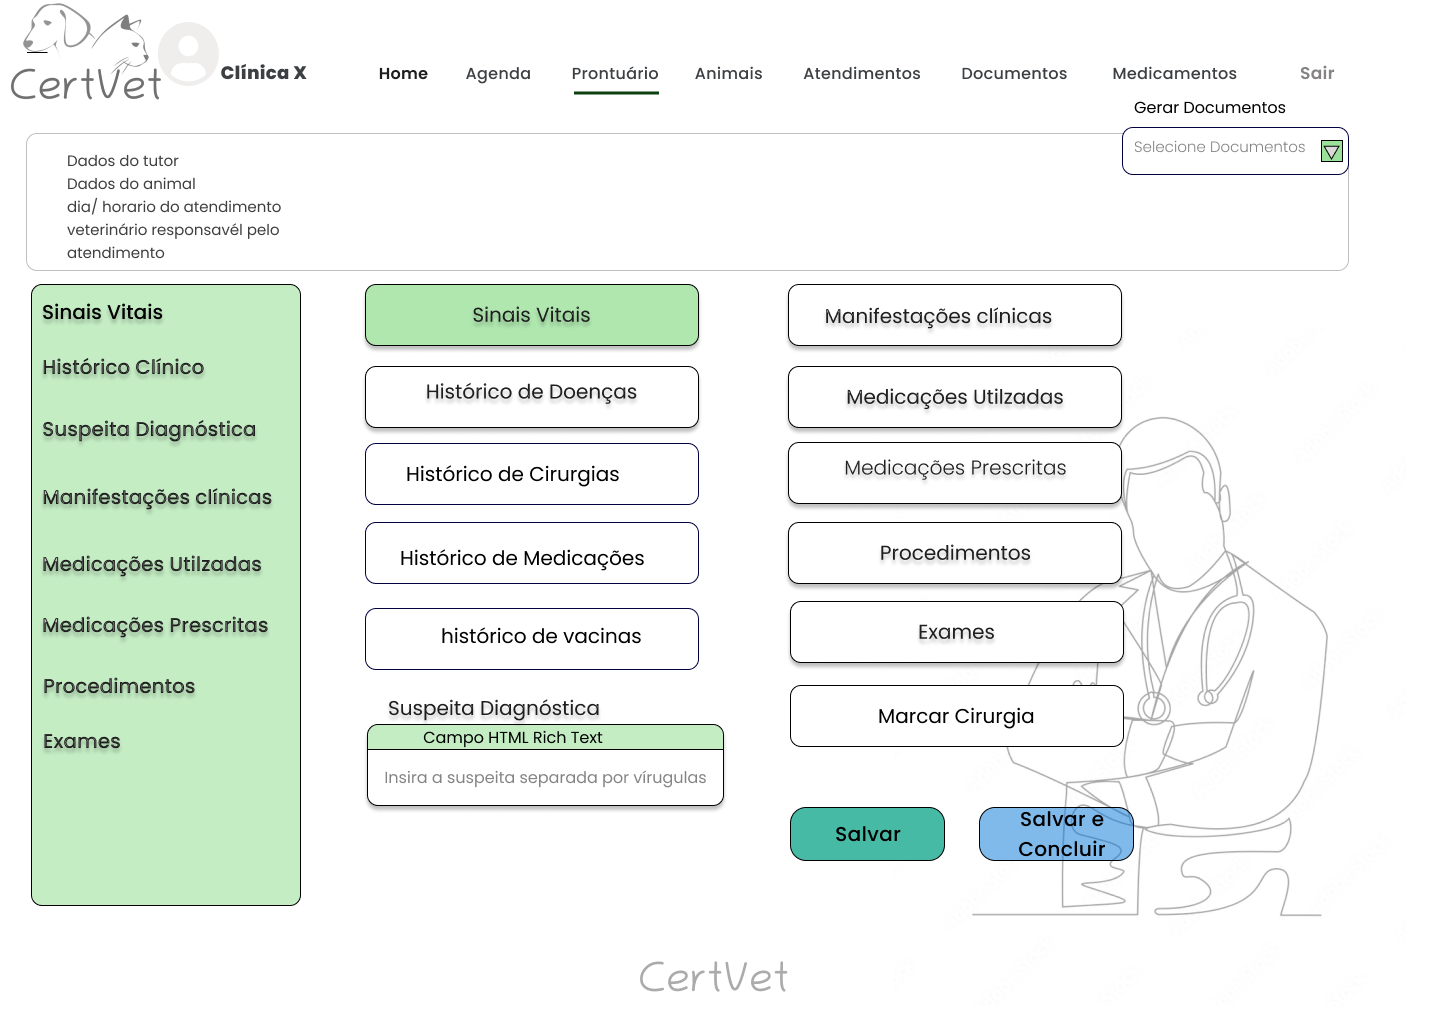
\includegraphics[width=0.7\textwidth]{images/Telas/Prontuario WF.png}

                \label{fig:ProntuarioWF}
                \centering
        {\footnotesize \DIFaddFL{Fonte: Elaborado pelos autores.}}
            \end{figure}    

\DIFadd{Os sinais vitais, por serem feitos em todas as consultas, independente do motivo que levou o animal ao atendimento, foi posicionado no alto da tela e seu preenchimento é feito de forma simples e direta, como podemos ver na figura \ref{fig:SinaisVitais}.
}

\begin{figure}[H]
                \centering
                \caption{\DIFaddFL{Tela de Prontuario - Sinais Vitais.}}
                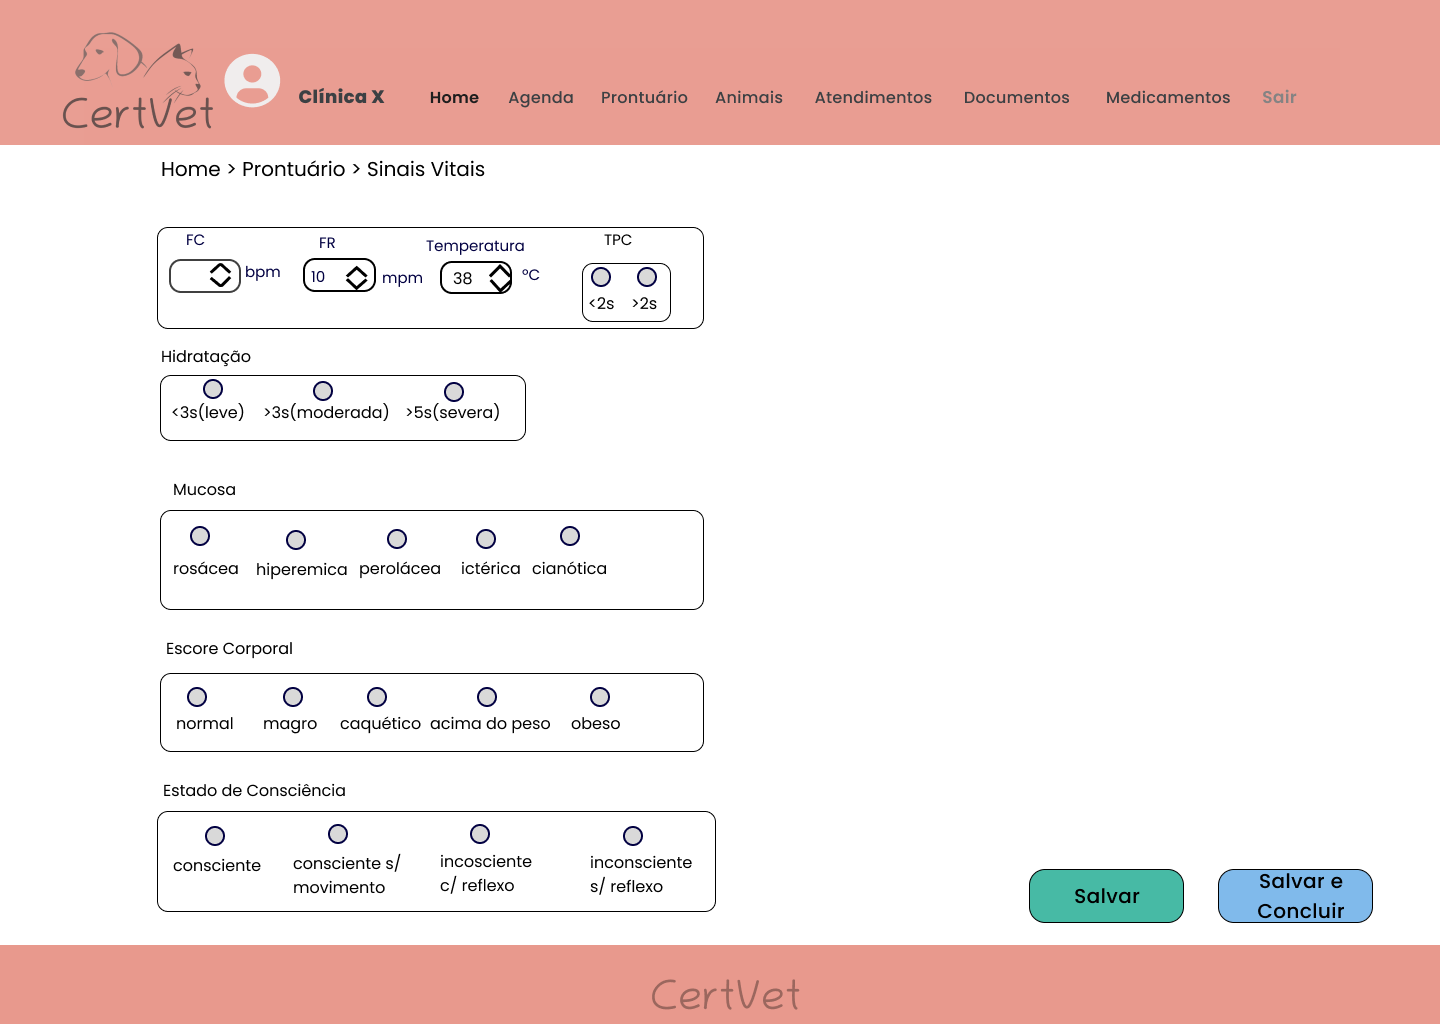
\includegraphics[width=0.7\textwidth]{images/Telas/Sinais Vitais.png}

                \label{fig:SinaisVitais}
                \centering
        {\footnotesize \DIFaddFL{Fonte: Elaborado pelos autores.}}
            \end{figure}    

\DIFadd{Outra seção que deve ser preenchida quando o animal apresenta alguma queixa é a de Manifestações Clínicas. Pensando novamente em facilitar o preenchimento e também pela existência ou não de todas as manifestões, optou-se por deixar a resposta negativa/nula como padrão, permitindo que o profissional apenas selecione as manifestações apresentadas que lhe são relevantes. Fig.: \ref{fig:Manifestacoes}. Quando necessário detalhar uma região específica, como no caso de dor ou sensibilidade e também em lesões e nódulos, abrem-se novos campos para selecionar tais regiões, como visto na figura \ref{fig:Regioes}. 
}

   \begin{figure}[H]
                \centering
                \caption{\DIFaddFL{Tela de Prontuario - Manifestações Clínicas.}}
                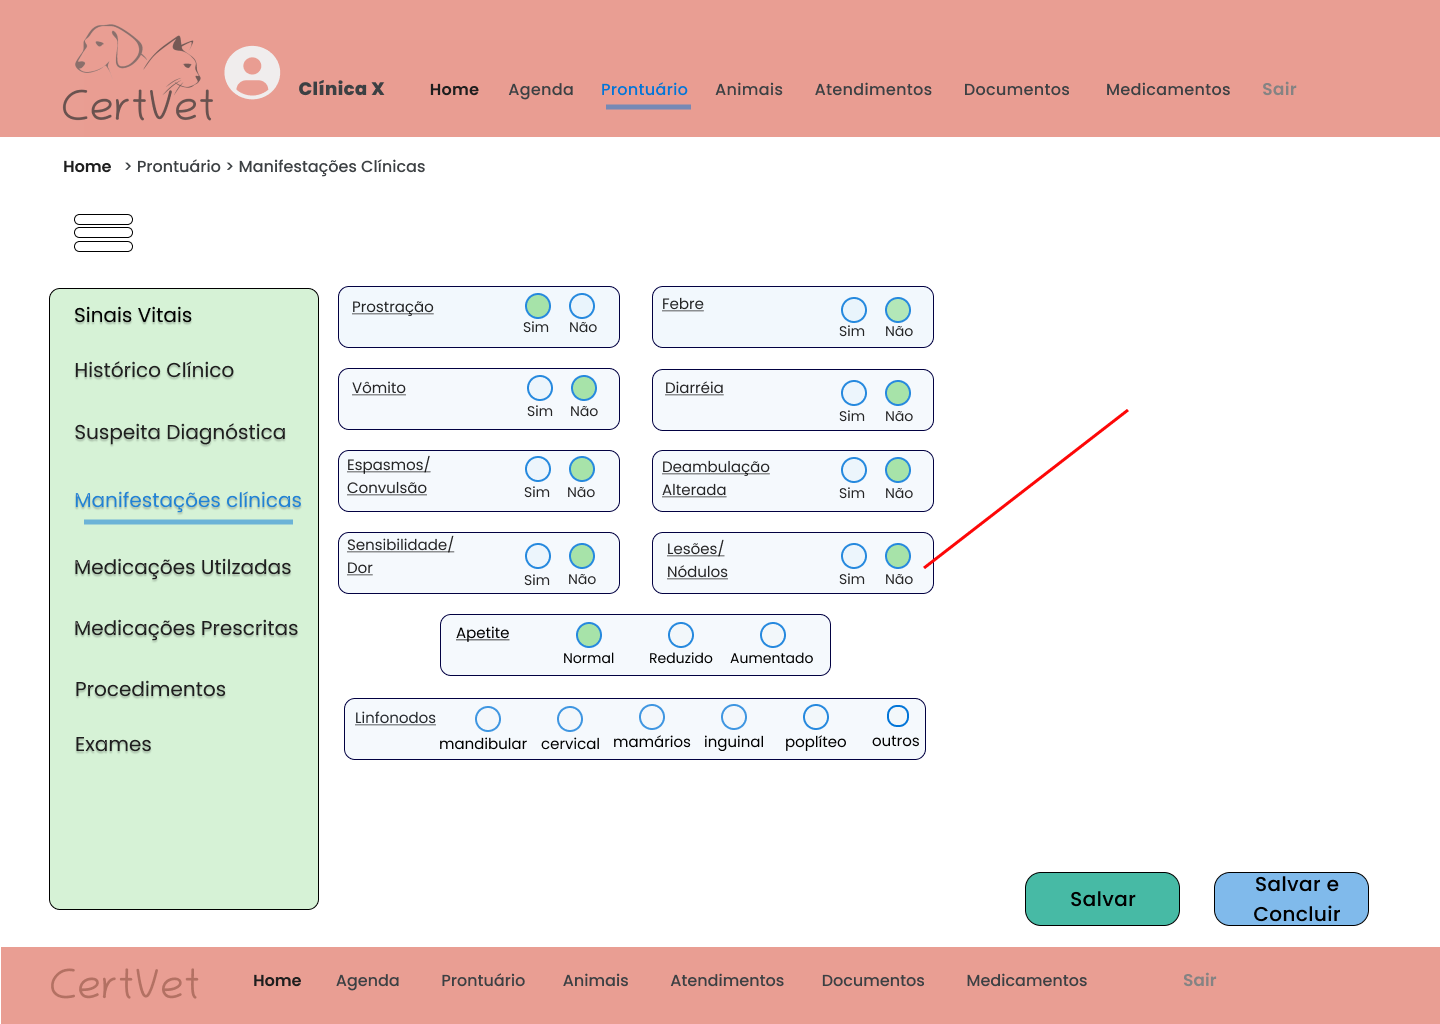
\includegraphics[width=0.7\textwidth]{images/Telas/Manifestacoes clinicas.png}

                \label{fig:Manifestacoes}
                \centering
        {\footnotesize \DIFaddFL{Fonte: Elaborado pelos autores.}}
            \end{figure}    

            \begin{figure}[H]
                \centering
                \caption{\DIFaddFL{Tela de Prontuario - Regiões Afetadas.}}
                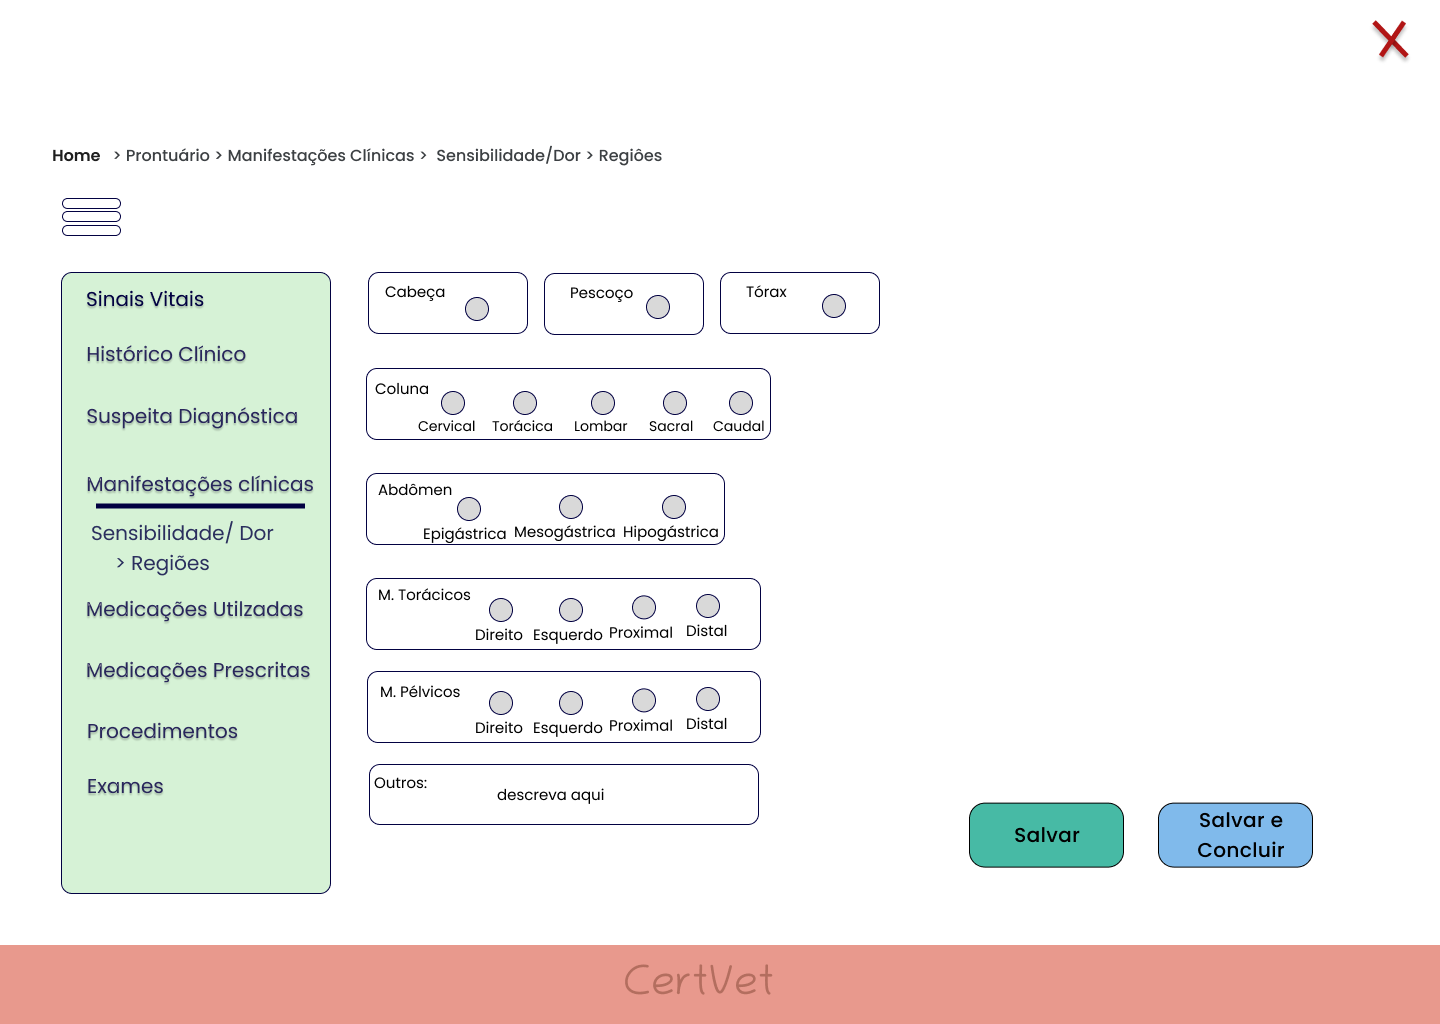
\includegraphics[width=0.7\textwidth]{images/Telas/Regioes.png}

                \label{fig:Regioes}
                \centering
        {\footnotesize \DIFaddFL{Fonte: Elaborado pelos autores.}}
            \end{figure}    

\DIFadd{Uma possível visão do documento final do Prontuário, após a finalização do atendimento é vista na figura \ref{fig:PdfProntuario}. Esta versão final do PDF gerado não pode ser editada e será válida como documento oficial.
}

    \begin{figure}[H]
                \centering
                \caption{\DIFaddFL{Visão Final do PDF do Prontuário.}}
                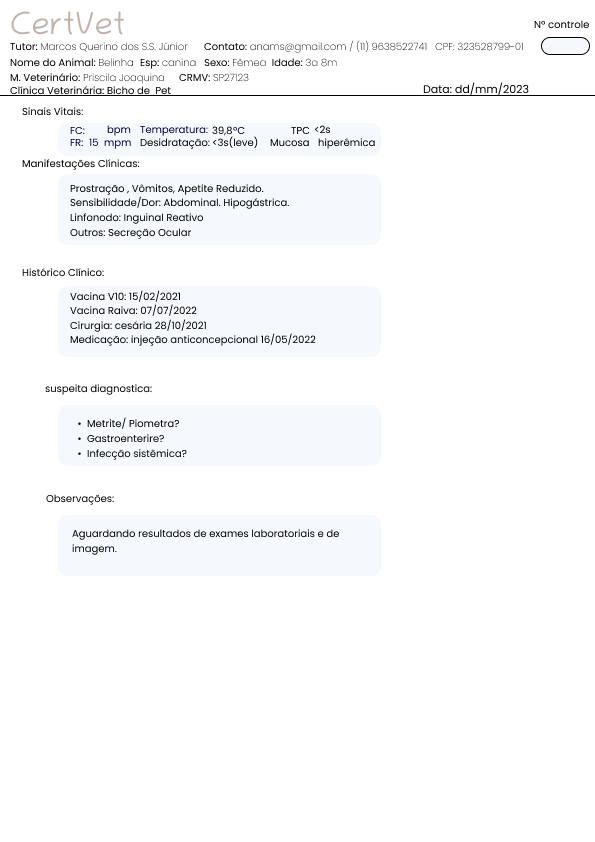
\includegraphics[width=0.7\textwidth]{images/Telas/PDF do Prontuario.png}

                \label{fig:PdfProntuario}
                \centering
        {\footnotesize \DIFaddFL{Fonte: Elaborado pelos autores.}}
            \end{figure}    

        











            
    
    %DIF >  Fim seção de TELAS %%%%


    \DIFaddend \section{Gestão e organização da equipe}

        \subsection{Organização da Equipe}

            O guia do \emph{\DIFdelbegin \DIFdel{scrum}\DIFdelend \DIFaddbegin \DIFadd{Scrum}\DIFaddend } declara explícitamente que o time deve ser pequeno suficiente para que seja ágil e grande o suficiente para que possa desempenhar trabalho relevante, recomendando o envolvimento de não mais que 10 integrantes \citeonline{scrum2}.

            Orientados pela recomendação de formação de papéis da equipe ágil \emph{Scrum}, foram definidos 3 papéis para ser desempenhado pelos membros da equipe: \emph{Product Owner} (PO -  Dono do Produto), \emph{\DIFdelbegin \DIFdel{scrum }\DIFdelend \DIFaddbegin \DIFadd{Scrum }\DIFaddend Master} (SCM - Mestre do Scrum) e \emph{Developers}, que foram denominados \emph{Team Members} (TM - Membros da equipe). Esses papéis têm o objetivo de apontar facilitadores e atribuir responsabilidades em pontos específicos do projeto, não havendo um responsável isolado ou encarregado do bom desenvolvimento das atividades.\citeonline{scrum2} \citeonline{agile2}

            O PO é responsável por definir clara e objetivamente como as funcionalidades da aplicação devem se comportar, compreender e priorizar a necessidade de negócio que melhor atende a necessidade do usuário (\emph{stakeholders}) e que o \emph{backlog }seja visível e disponível para todos os membros do time.\citeonline{agile2} O papel será desempenhado pela Irina Chang.

            O SCM tem a responsabilidade que o time consiga desenvolver autonomia, destravando entendimentos e facilitando a identificação de dinâmicas que resultem em melhor entregabilidade das atividades.\citeonline{agile2} O papel será desempenhado por Henrique.

            \emph{Team Member} é a forma como foi decidido denominar o papel dos desenvolvedores. Estes serão os responsáveis pela implementação de código, padronização de commits, integrações, modelagem de banco de dados, além de verificar se as alterações propostas pelo PO são tecnicamente viáveis de serem implementadas, definindo os processos necessários para a implementação. Por consequência, são os maiores responsáveis pelo desenvolvimento da documentação do código e garantia da manutenibilidade. Independentemente do envolvimento anterior, são responsáveis por auxiliar em  manutenções futuras e realizar a entrega (\emph{deploy}) da aplicação em produção.\citeonline{scrum2} Os team members são: Caique Daniel, Luis Renato, Marcos Querino, Murilo Pires e Welen Mota.

            Entretanto, diferentemente do papel do Scrum, o time conta com indivíduos com conhecimentos e habilidades diversas e tempo limitado para o desenvolvimento do projeto. Dessa forma, os papeis servirão como referência, mas não limitam os indivíduos às atividades definidas pelos papéis do Scrum.

            Todos os membros escreveram diferentes partes da documentação, textos que eram revisados posteriormente pelos outros integrantes. O controle de versionamento também foi tarefa de todos os integrantes. A geração de métricas e envios para versionamento na SVN, apesar de ser de conhecimento de todos, mas devido a diferentes problemas técnicos enfrentados por alguns integrantes, não pode ser efetuada por todos os membros. A correção dessas falhas estão planejadas para o período de recesso do ano letivo, para não atrapalhar o andamento do resto do projeto. O desenvolvimento da parte técnica do projeto, relativo a codificação (\emph{front-end} e \emph{back-end}) e infraestrutura levou em conta o conhecimento prévio de cada integrante, sua familiaridade com as tecnologias e capacidade de desenvolver a aplicação em tempo hábil. Com isso, alguns membros com menor grau de familiaridade com a tecnologia, participavam dos \emph{pair-programming} como observadores, ajudando a identificar possíveis erros no código, o que contribuiu para maior aprendizado dos mesmos e aprofundar o conhecimento de todos em todas as partes do projeto.

             O Quadro \ref{tab:membros} foi elaborado para facilitar a identificação da ênfase de atuação de cada indivíduo sobre as atividades desempenhadas.

        \begin{center}
            \begin{quadro}[H]
            \centering
            \caption{Membros}
            \resizebox{16cm}{!}{%
                \begin{tabular}{|p {15}|rrrrrrrr|}
                \hline
                \multicolumn{1}{|c|}{Membro}      & \multicolumn{1}{c|}{Irina}   & \multicolumn{1}{r|}{Henrique} & \multicolumn{1}{r|}{Caique}       & \multicolumn{1}{r|}{Luís} &
                \multicolumn{1}{r|}{\begin{tabular}[c]{@{}c@{}}Marcos \end{tabular}}  &
                \multicolumn{1}{r|}{Murilo} & \multicolumn{1}{r|}{Welen}\\ \hline

            \multicolumn{1}{|l|}{\begin{tabular}[c]{@{}c@{}}Documentação \end{tabular}} &
            \multicolumn{1}{c|}{x}  & \multicolumn{1}{c|}{x}  & \multicolumn{1}{c|}{x}  & \multicolumn{1}{c|}{x}  & \multicolumn{1}{c|}{x}  & \multicolumn{1}{c|}{x}  & \multicolumn{1}{c|}{x}            \\ \hline

        \multicolumn{1}{|l|}{\begin{tabular}[c]{@{}c@{}}Versionamento \end{tabular}} &
            \multicolumn{1}{c|}{x}  & \multicolumn{1}{c|}{x}  & \multicolumn{1}{c|}{x}  & \multicolumn{1}{c|}{x}  & \multicolumn{1}{c|}{x}  & \multicolumn{1}{c|}{x}  & \multicolumn{1}{c|}{x}            \\ \hline
            \multicolumn{1}{|l|}{\begin{tabular}[c]{@{}c@{}}Métricas\end{tabular}} &
             \multicolumn{1}{c|}{x}  & \multicolumn{1}{c|}{x}  & \multicolumn{1}{c|}{ }  & \multicolumn{1}{c|}{ }  & \multicolumn{1}{c|}{ }  & \multicolumn{1}{c|}{ }  & \multicolumn{1}{c|}{x}            \\ \hline
        \multicolumn{1}{|l|}{\begin{tabular}[c]{@{}c@{}}\emph{Front-end} \end{tabular}}&                 
            \multicolumn{1}{c|}{ }  & \multicolumn{1}{c|}{ }  & \multicolumn{1}{c|}{ x }  & \multicolumn{1}{c|}{x}  & \multicolumn{1}{c|}{x}    & \multicolumn{1}{c|}{ }  & \multicolumn{1}{c|}{ }            \\ \hline

        \multicolumn{1}{|l|}{\begin{tabular}[c]{@{}c@{}}\emph{Back-End} \end{tabular}} &
            \multicolumn{1}{c|}{x} & \multicolumn{1}{c|}{x}  & \multicolumn{1}{c|}{} & \multicolumn{1}{c|}{}  & \multicolumn{1}{c|}{} & \multicolumn{1}{c|}{x}  & \multicolumn{1}{c|}{}            \\ \hline

    \multicolumn{1}{|l|}{\begin{tabular}[c]{@{}c@{}}Banco de dados \end{tabular}} &
            \multicolumn{1}{c|}{}  & \multicolumn{1}{c|}{}  & \multicolumn{1}{c|}{x} & \multicolumn{1}{c|}{}  & \multicolumn{1}{c|}{}  & \multicolumn{1}{c|}{}  & \multicolumn{1}{c|}{}            \\ \hline

        \multicolumn{1}{|l|}{\begin{tabular}[c]{@{}c@{}}Infraestrutura \end{tabular}} &
            \multicolumn{1}{c|}{ }  & \multicolumn{1}{c|}{x} & \multicolumn{1}{c|}{ } & \multicolumn{1}{c|}{ } & \multicolumn{1}{c|}{ } & \multicolumn{1}{c|}{ }  & \multicolumn{1}{c|}{ }            \\ \hline

    \end{tabular}%
       }
        \label{tab:membros}
        \centering

        {\footnotesize Fonte: Elaborado pelos autores.}
        \end{quadro}
    \end{center}

            % Fonte: https://scrumguides.org/scrum-guide.html#scrum-team
            % Fonte https://www.atlassian.com/br/agile/scrum/roles
            % Revisão fim %  


    \subsection{Gestão de projeto}

        % Revisão inicio %
        %Estou com duvidas com relação a esse primeiro paragrafo
        %A partir da avaliação dos requisitos, considerou-se que não existem funcionalidades com processos claramente definidos até o início do desenvolvimento de cada processo e o tempo hábil para elaborar e documentar extensamente todos os processos para serem implementados não é suficiente para que exista código a ser implementado. Portanto, a abordagem de planejamento de projetos cascata não é adequada para desenvolver a solução.

        Considerando a restrição temporal definida pelo cronograma acadêmico e os Requisitos Funcionais e Requisitos Não Funcionais já expostos anteriormente nos Quadros \ref{tab:req_func} e \ref{tab:req_nfunc} respectivamente, a equipe decidiu que adotar alguns elementos da metodologia \emph{Scrum} \citeonline{scrum} e a prática do \emph{pair programming} do \emph{Extreme Programming} (XP) \citeonline{agile} seriam melhor adequados às necessidades do projeto. Enfatizando o emprego dos processos, rituais e cerimônias do \emph{Scrum} e apenas complementando com um elemento do método XP para o dia a dia de desenvolvimento, fomentando maior propensão à colaboração e dinamismo de desenvolvimento entre os membros da equipe, resultando em entregas com ritmo constante e incremental.

        %mudar sprint para : \emph{sprint} para transformar em itálico 

        Os ciclos para o desenvolvimento do projeto foram projetados com duração semanal, denominadas \emph{sprint}. Este processo é definido no \emph{Scrum} como o período em que ocorrem os desenvolvimentos, sendo um dos conceitos centrais da metodologia. Define o escopo que será trabalhado, movendo os itens que passam do \emph{backlog} para a etapa de refinamento e desenvolvimento pela equipe, analisa e desenvolve os elementos que comporão a solução, podendo negociar novos prazos com o PO conforme a equipe identifica novos aprendizados \citeonline{scrum}. Este processo permite melhor acompanhamento da evolução do desenvolvimento, permitindo manter os \emph{stakeholders} atualizados e com expectativas alinhadas.

        Ao final de cada \emph{sprint}, ocorre a cerimônia de \emph{Sprint Review} para discutir o processo de aprendizado do período, quais os resultados obtidos e avaliar a evolução da semana, através de debate sobre dificuldades, soluções e impedimentos encontrados no decorrer da \emph{sprint}. Também é realizado o planejamento da \emph{sprint} da semana seguinte, analisando e priorizando os próximos itens que passarão do \emph{backlog} para serem trabalhados no próximo ciclo de desenvolvimento durante as \emph{sprint plannings}, conforme a recomendações de \citeonline{scrum} para o Scrum.

        A prática de \emph{pair programing} é adotada para estimular o desenvolvimento colaborativo no time, tal abordagem permite maior compartilhamento dos conhecimentos de cada indivíduo, de forma mais coesa e analisada por pares durante o desenvolvimento do código ou documento. Tal abordagem reduz possíveis atrasos no desenvolvimento decorrentes de dúvidas ou entraves individuais, tendo como consequência a entrega de código com consistência e validação por pares. A abordagem também aumenta o envolvimento do time em relação a entrega de código com qualidade, derivado do sentimento de responsabilidade coletiva que nasce da autonomia para modificações \citeonline{agile}.

        A abordagem aprofunda o conhecimento específico da equipe sobre determinado assunto e da solução construída e incentiva o compartilhamento e comunicação entre os integrantes envolvidos imediatamente durante o desenvolvimento ou durante a \emph{sprint review}.

        Nos Quadros \ref{qd:sprints}, \ref{qd: epic} e \ref{qd: backlog} estão relacionadas as informações de desenvolvimento do projeto referentes às \emph{sprints} semanais, divisão de tarefas \emph{Epics} e o \emph{product backlog} do desenvolvimento do projeto.
        % Revisão fim %
        \begin{center}
      \begin{quadro}[H]
      \centering
          \caption{\emph{Sprints}}
          \begin{tabulary}{1.0\textwidth}{|p{8em}|p{8em}|p{19em}|}
        \hline
        Início & Fim & Descrição\\
        \hline
        09/08/2022/ & 16/08/2022 & Definição de grupo e discussão inicial sobre temas. \\
        \hline
        16/08/2022 & 23/08/2022 & Apresentação das propostas aos professores e escolha do projeto.\\
        \hline
        23/08/2022 & 30/08/2022 & Apresentação inicial dos projetos, aprovação do tema e divisão das atividades.\\
        \hline
        30/08/2022 & 06/09/2022 & Início da modelagem da aplicação.\\
        \hline
        06/09/2022 & 13/09/2022 & Início do desenvolvimento da modelagem de dados.\\
        \hline
        13/09/2022 & 20/09/2022 & Escolha da arquitetura da aplicação.\\
        \hline
        20/09/2022 & 27/09/2022 & Discussão de Regras de negócio, Requisitos e Custo do Projeto. \\
        \hline
        27/09/2022 & 04/10/2022 & Apresentação do Desenho da aplicação e definição dos próximos passos. \\
        \hline
        04/10/2022 & 11/10/2022 & Semana de desenvolvimento e preparação para a apresentação da POC. \\
        \hline
        11/10/2022 & 18/10/2022 & Ajustes finais para a apresentação da POC. \\
        \hline
        18/10/2022 & 25/10/2022 & Hands on de implementações e ajustes de documentação.\\
        \hline
        25/10/2022 & 01/11/2022 & Discussão e desenvolvimento da documentação e evolução do MVP da aplicação. \\
        \hline
        01/11/2022 & 08/11/2022 & Desenvolvimento final da documentação e da aplicação do MVP.\\
        \hline
        \end{tabulary}

          \label{qd:sprints}
          \centering
         { \footnotesize Fonte: Elaborado pelos autores.}
      \end{quadro}
    \end{center}  

    %  Criação do backlog  %

 \begin{center}
      \begin{quadro}[H]
      \centering
          \caption{\emph{Epics}}
          \begin{tabulary}{1.0\textwidth}{|p{12em}|p{25em}|}
        \hline
       Epic & Descrições  \\
        \hline
        Ajustes Documentação & Mudanças ao longo do projeto na documentação (documentação como um todo)\\
        \hline
        Ajustes Administrativos & Atualizações Gource, SVN, Métricas, posts no blog\\
        \hline
        Desenvolvimento POC &\emph{Front-end}: funcionalidades\emph{Front-end} desenvolvidas na POC.
        \emph{back-end}: funcionalidades \emph{back-end} desenvolvidas na POC\\
        \hline
        Desenvolvimento MVP &\emph{Front-end}: funcionalidades front end desenvolvidas no MVP.
      \emph{back-end}: funcionalidades back end desenvolvidas no MVP\\
        \hline
        \end{tabulary}
          \label{qd: epic}
          \centering
         { \footnotesize Fonte: Elaborado pelos autores.}
      \end{quadro}
    \end{center} 


    \begin{center}
      \begin{quadro}[H]
      \centering
          \caption{\emph{Product Backlog}}
          \begin{tabulary}{1.0\textwidth}{|p{6em}|p{5em}|p{24em}|}
        \hline
       Entregar até & Prioridade & Descrição \\
        \hline
         30/08/2022 & Alta & Definir tema final que será desenvolvido no projeto, realizar apresentação do tema definido\\
         \hline
         13/09/2022 & Alta & Realizar a modelagem do MER e DER para suportar a aplicação, validar com os clientes\\
         \hline
         20/09/2022 & Alta & Realizar o desenho de arquitetura do sistema, validar com os integrantes do time as tecnologias utilizadas, validar com os clientes.\\
        \hline
         27/09/2022 & Alta & Definir regras de negócios do sistema, definir requisitos funcionais, casos de uso, histórias de usuários, custos do projeto\\
         \hline
         27/09/2022 & Alta & Configurar ambiente RDS; Configurar Docker; Configurar aplicações em springboot; Configurar aplicações em React\\
        \hline
        11/10/2022 & Alta & Desenvolver funcionalidades de autenticar usuário e registrar usuário no banco de dados na AWS. \\
        \hline
        11/10/2022 & Media & Entregar funcionalidades registro CRMV, entendimento da viabilidade da funcionalidades, alinhar por e-mail com a CFMV.\\
        \hline
         18/10/2022 & Alta & Entregar funcionalidades levantadas no escopo da POC, apresentar para os clientes as funcionalidades.\\
        \hline
         25/10/2022 & Alta & Realizar ajustes e correções da POC, Realizar melhorias na proposta da aplicação, realizar ajustes na documentação com o feedback dos clientes \\
        \hline
        01/11/2022 & Alta & Realizar desenvolvimento funcionalidades x (MVP)
        desenvolvimento funcionalidades y (MVP)
        Ajustes finais na documentação\\
        \hline
         08/11/2022 & Alta & Entrega da documentação do projeto, feedbacks do cliente e definições para a apresentação do MVP\\
        \hline
        22/11/2022 & Alta & Entrega da apresentação do MVP e feedback dos clientes.\\
        \hline
        \end{tabulary}

          \label{qd: backlog}
          \centering
         { \footnotesize Fonte: Elaborado pelos autores.}
      \end{quadro}
    \end{center}

    % % % %  

    \subsection{Ferramenta de gestão}

        Após definir as funcionalidades que seriam desenvolvidas, foi constatada a necessidade de geri-las a partir de uma ferramenta de gestão de projetos.

        Sistemas como Microsoft Project e similares são ideais para projetos que empregam a abordagem do modelo cascata. Como não proveem a flexibilidade para mudanças e velocidade de aprendizado que projetos ágeis exigem, optou-se pelo uso da ferramenta Jira Software, disponível no modelo gratuito e \emph{on cloud}.

        Como ferramenta de mercado, o Jira Software é uma ferramenta de gestão de projetos flexível, reconhecida por dar suporte a diferentes abordagens de gestão de projeto, mas comumente utilizada em projetos que envolvem metodologias ágeis, \citeonline{jira}.

        No contexto do desenvolvimento da aplicação, as atividades foram divididas em Épicos, que contêm Histórias e Tarefas distribuídas por quadros \emph{Kanban}. Estes quadros permitem maior flexibilidade nos processos de gestão das atividades, organizando o fluxo de trabalho com as tarefas planejadas, em progresso e entregues, \citeonline{jira}.

        % Revisão fim %  

    \section{Arquitetura}

        % Revisão inicio %

        %O sistema foi desenvolvido com base no modelo de arquitetura cliente-servidor, abordando a divisão de camadas e a separação no que consiste em \emph{back-end} e\emph{ Front-end} da aplicação. Por meio de um navegador web, os clientes fazem as requisições ao servidor, que é acessível através de uma API (Application Programming Interface) REST responsável por lidar com as regras de negócio e com a comunicação entre as camadas. O Elastic Load Balancing tem como responsabilidade distribuir esse tráfego de entrada entre as duas instâncias EC2, uma contendo o back end e outra o front end, ambas em ambientes isolados pelo Docker Container, onde o back end possui integrado a ele o CloudWatch Logs para monitoramento dos logs da aplicação. Toda essa parte de serviços operacionais do sistema está inclusa no AWS Elastic BeanStalk, provedor de máquina e serviços necessários de forma a abstrair detalhes de infraestrutura para a implementação da aplicação.

        %Como banco de dados relacional da aplicação, foi empregado o serviço gerenciado de banco de dados AWS RDS para MySQL. Este serviço permite o funcionamento do banco de forma abstraída, enquanto, para o armazenamento de arquivos estáticos da aplicação, como os documentos pdf emitidos pela aplicacão CertVet, foi empregado o serviço Amazon S3.

        

        % Antes %
        % ------------- %
        % Depois %

        A aplicação está hospedada na infraestrutura da provedora de nuvem pública AWS. A provedora fornece todos os recursos computacionais e serviços necessários para que a solução seja executada, além de prover Virtual Private Cloud (VPC), que atua como rede interna e \emph{Security Groups}, que atua como \emph{firewall}.

        O sistema foi desenvolvido com base no modelo de arquitetura cliente-servidor, empregando a abordagem de divisão em camadas \emph{Back-End} e \emph{Front-End} para maior desacoplamento.

        O cliente, via navegador web, efetua uma requisição ao endereço da CertVet e acessa à aplicação front-end hospedada em sua respectiva instância EC2, que permite que seja processada pelo próprio navegador.

        Por meio da interface web, as diversas intâncias dos clientes fazem requisições ao servidor, utilizando o padrão Representational State Application Programming Interface (REST API).
        Assim, o servidor presente na instância EC2 que executa o \emph{container} da aplicação \emph{Java Spring Boot} fica responsável por resolver as regras de negócio e comunicar seus resultados entre as demais camadas.

        Como parte da integração com terceiros, a aplicação de \emph{back-end} prevê realizar requisições ao servidor externo de domínio da entidade de classe CRMV.
        %\emph{container} 

        O serviço Elastic Load Balancing tem como responsabilidade distribuir o tráfego de dentro e fora da VPC entre as possíveis instâncias EC2 que processam as requisições da aplicação e seus clientes, em caso de escalonamento vertical ou horizontal da aplicação.

        Para que seja possível armazenar os \emph{logs}da aplicação, o \emph{back-end} está integrado ao serviço \emph{CloudWatch Logs}. Este serviço permite que os \emph{logs}da aplicação possam ser monitorados de fora do servidor de instalação da aplicação.

        O serviço operacional é provisionado pelo AWS Elastic BeanStalk, que abstrai o processo de requisição e reserva de recursos de infraestrutura que implementa da aplicação.

        O sistema de gerenciamento de banco de dados relacional responsável pelo armazenamento dos dados da aplicação é o MySQL provido pelo AWS RDS, serviço gerenciado que persiste os estados gerados pela lógica de negócio de forma abstraída, enquanto, para o armazenamento de arquivos estáticos da aplicação, como os documentos gerados pela aplicação CertVet, fora utilizado o armazenamento de objetos Amazon S3 como banco de dados não relacional.

        Para armazenamento das imagens da solução, está previsto o serviço da provedora Docker, mas não é restrito a este provedor.

        A Figura \ref{fig:infra3} ilustra a arquitetura planejada e implementada para a CertVet, utilizando as tecnologias já citadas anteriormente.

        % Revisão fim %   

        \begin{figure}[H]
            \centering
            \caption{Versão Final do Esquema de Infrastrutura}
            \centering
            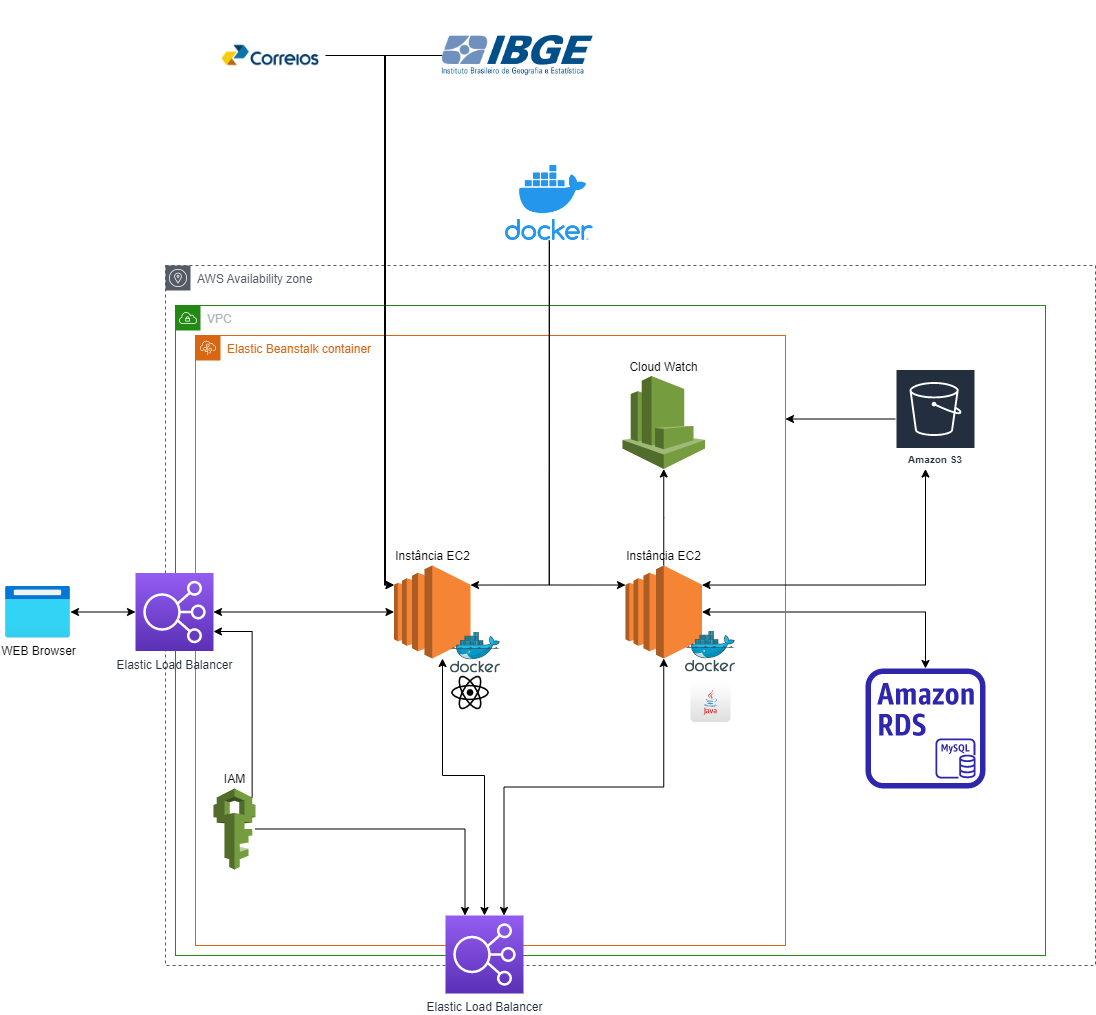
\includegraphics[width=0.65\textwidth]{images/ArquiteturaAplicacao_v6.png}
            \label{fig:infra3}
        \end{figure} 

        \subsubsection{Elastic Load Balancing}

            Serviço que distribui o tráfego externo à infra estrutura entre instâncias de processamento da aplicação. Em diversos cenários de aplicações, a tecnologia permite que uma solução seja escalável de forma horizontal para um numero de instâncias de tamanhos variáveis de acordo com a parametrização do gestor da solução \citeonline{eld}.

        \subsubsection{Docker Container}

            Tecnologia que isola o ambiente da aplicação através da segregação de recursos em namespaces e imagem de aplicação, permitindo maior liberdade no uso dos recursos computacionais de execução em ambiente isolado e portabilidade \citeonline{docker}.

            Normalmente toma como ponto de partida a distribuição Alpine Linux, que tem o objetivo de ter apenas os recursos necessários para o sistema operacional, aumentando o controle do desenvolvedor sobre os utilitários do sistema operacional.

            Para a aplicação \emph{back end}, será empregada uma imagem baseada na pilha Amazon, Linux e Amazon Corretto 17.

        \subsubsection{AWS Elastic BeanStalk}

            Serviço gerenciado que abstrai a necessidade de tomar decisão sobre recursos físicos da aplicação, provisionando máquina e serviços necessários para a implementação da solução. Provê suporte à tecnologia Docker \emph{container} \citeonline{elbean}.

        \subsubsection{Amazon ECR - Amazon Elastic Container Registry}

            Similar ao serviço Docker Hub, é um serviço de armazenamento e registro de imagens de containers gerenciado pelo provedor AWS. Permite que seja possível realizar implantações (\emph{deploy}) automatizados a partir da atualização da imagem Docker armazenada no diretório em nuvem \citeonline{ecr}.

        \subsubsection{AWS RDS (Relational Database Service) - Amazon AWS}

            Serviço gerenciado que provê banco de dados com redundância em infraestrutura abstraída, suporta implementações de banco de dados relacionais: Amazon Aurora, MySQL, MariaDB, PostgreSQL, Oracle e Microsoft SQL Server. Disponibiliza as funcionalidades de uso mais recorrentes por aplicações \citeonline{rds}.

            Para a implementação da solução, identificou-se que o uso de uma instância MySQL se enquadra melhor às necessidades da aplicação por não existir necessidade imediata de atender altos volume de transações com o banco de dados.

        \subsubsection{Amazon S3}

            Serviço de armazenamento de objetos (no caso da Certvet, documentos de resultado de exames) que oferece escalabilidade \citeonline{s3}. 

    \section{Tecnologias de Desenvolvimento}

        Aproveitando da maturidade de \emph{frameworks} e bibliotecas \emph{front-end} e a complexicidade adicional do desenvolvimento de aplicações dedicadas para ambientes \emph{desktop} e móveis, com ênfase em celulares (necessidade de permissão de máquina para instalação e configuração da aplicação em ambiente heterogêneo além de particularidades pontuais de cada cliente), o foco da aplicação foi voltado para a plataforma WEB (navegadores \emph{desktop} e móveis).

        Para prototipação, foi utilizada a ferramenta Figma, um editor colaborativo \emph{online} de \emph{design} gráfico que permite a criação de interfaces de usuário. A ferramenta auxilia desenvolvedores a construir telas coesas e baseadas nos conceitos e práticas de \emph{User Experience} (UX) e \emph{User Interface }(UI). Como ferramenta de desenvolvimento, a plataforma GitHub será usada como principal ferramenta de versionamento dos  repositórios do projeto.

        Com o objetivo de facilitar o processo de implementação de uso da ferramenta nos estabelecimentos dos usuários, a instalação de um software como aplicação \emph{desktop} poderia influenciar negativamente à adoção da aplicação. Ainda, de acordo com as habilidades técnicas dos membros da equipe, foi optado por utilizar tecnologias web baseadas em servidores de aplicação remotos e gerenciados, oferecendo o software como serviço (\emph{Software as a Service - SaaS}).

        A oferta de software como serviço permite que atualizações e correções sejam implementadas mais rapidamente por não depender da interferência em infraestrutura de responsabilidade do cliente. Adicionalmente, reduz-se o risco de instalação do serviço de forma inadequada.

    \subsection{\emph{Front-end}}

        A pilha de tecnologias de desenvolvimento para o \emph{front-end} se concentram nas ferramentas e tecnologias:

        \begin{itemize}

            \item Figma: Editor colaborativo \emph{online} de \emph{design} gráfico que permite a criação de interfaces de usuário e que ajudará os desenvolvedores a construir telas coesas e baseadas nos conceitos e práticas de \emph{User Experience} (UX) e \emph{User Interface} (UI).\citeonline{figma}

            \item Typescript:
                Linguagem que permite programação fortemente tipada de código aberto desenvolvida pela Microsoft lançada em 1 de outubro de 2012. \citeonline{ts}

                É também um supertipo da linguagem  JavaScript, o que significa que possui todas as funcionalidades do JavaScript e além da adição de novos recursos. 

                Essa linguagem foi selecionada para desenvolver o \emph{front end} devido à complexidade e escala da aplicação, que requer estruturas de dados mais complexas do que o JavaScript pode oferecer suporte, fazendo-se necessário a utilização de uma linguagem com tipagem de dados forte. 

                Outro motivo que colaborou para a escolha foi a segurança, já que graças a tipagem de dados, erros que podem causar vulnerabilidades e passam despercebidos em aplicações desenvolvidas com JavaScript serão identificados no momento da compilação do TypeScript para JavaScript.

            \item SCSS:
                Linguagem de estilização para WEB compilada para CSS.

                Essa linguagem foi selecionada para estilizar o \emph{front end} da aplicação pelo fato de possuir compatibilidade com o CSS e também uma melhor estrutura organizacional de código quando comparado com o CSS.\citeonline{scss}

            \item ReactJS:
                Biblioteca JavaScript/TypeScript desenvolvida pelo Facebook para a criação de interfaces WEB lançada em 29 de maio de 2013. O React foi escolhido graças a arquitetura baseada em componentes que permite a reutilização dos mesmo em diferentes partes da aplicação. Os componentes são escritos utilizando JSX que possui uma sintaxe semelhante ao HTML, o que o torna fácil de utilizar.\citeonline{reactjs}

            \item Bootstrap:
                \emph{Framework front-end} que fornece estruturas de CSS para a criação de sites e aplicações responsivas de forma rápida e simples.\citeonline{bootstrap}

                Essa tecnologia foi escolhida pelo fato de reduzir consideravelmente o tempo de desenvolvimento da estilização da interface da aplicação com om usuário.

        \end{itemize}  

        \subsection{\emph{Back-End}}

            Para compor a pilha de tecnologias aplicadas no \emph{back-end}, foi definido utilizar as seguintes tecnologias:

            \begin{itemize}
                \item Java 17: 
                    Linguagem de programação fortemente tipada com ênfase no paradigma de desenvolvimento orientado a objeto. Habitualmente empregada em aplicações comerciais e cientificas maduras, tanto open source como privadas.\citeonline{java}

                    A partir da comunidade de desenvolvimento, projetos open source de permissionamento livre permite acesso a bibliotecas e ferramentas como \emph{framework} Demoiselle, para assinatura de documentos que cumprem a especificação ICP-Brasil.

                    A versão 17 é uma versão LTS - Long Term Service, permite o emprego das tecnologias e funcionalidades mais recentes da linguagem, sem prejuízo às implementações mais antigas.

                \item \emph{Framework}Spring Boot: 
                   \emph{ Framework} comumente utilizado da linguagem Java para aplicações de uso geral, permite integração sem quebras entre dependências de bibliotecas e frameworks especializados como Spring MVC, hibernate ou Apache Kafka \citeonline{spring}.
                    \begin{itemize}
                        \item ORM - spring JPA (Hibernate)
                        \item Spring Web - \emph{controllers}
                        \item Apache Tomcat - Servidor HTTP
                        \item Hibernate Validator
                        \item Mockito - \emph{Framework} que auxilia o desenvolvimento de testes de unidade
                        \item SL4J - \emph{Framework} dedicado ao registro de \emph{logs}
                    \end{itemize}
                \item SGBD MySQL:
                    Sistema de gerenciamento de banco de dados relacional com ampla implementação de provedores de tecnologias em nuvem aberta ou on premisses, tendo licença permissiva de uso e familiaridade aos membros da equipe.

                \item Postman:
                Ferramenta que permite realizar solicitações HTTP e requisições a fim de testar a API a partir de análises de suas respostas. Além disso, permite a depuração de testes de forma mais facilitada e a realização de testes de automação, auxiliando na garantia do funcionamento esperado por parte da API. 

                \item Swagger:
                \emph{Framework} que promove a organização das rotas através de documentações e geração de códigos cliente e servidor, seja de forma automática ou manual, \citeonline{swagger}.

            \end{itemize} 

        \subsection{Ferramentas de testes automatizados}

            Com o objetivo de testar a aplicação e também garantir que as funções retornem os resultados esperados de forma a garantir a integração das partes da mesma, teste unitários são fundamentais para alcançar esses objetivos. Portanto, a equipe utilizará as ferramentas de testes automatizados listados a seguir:

            \begin{itemize}
                \item Jest: é um \emph{framework} de testes para JavaScript/TypeScript desenvolvido a partir do \emph{framework}Jasmine, também para testes automatizados.
                \item JUnit: é um \emph{framework} open-source de teste para a linguagem Java desenvolvido por Erich Gamma e Kent Beck. é assumido por padrão pelo \emph{framework} Spring e suas ferramentas (Spring Boot).
            \end{itemize}    

%\subsection{Integrações existentes}

    %O sistema utiliza integração com a API dos Correios para preenchimento automático do endereço após a inserção do código de CPF do usuário, otimizando a experiência deste.


    \section{Manutenibilidade}
    Visando garantir boa resposta dos clientes, atingindo um elevado nível de qualidade, torna-se necessário estabelecer determinados requisitos e parâmetros de manutenibilidade e ferramentas que possam auxiliar esse processo. Partindo desses critérios, é possível mensurar o quanto o desenvolvimento do sistema apresenta conformidade com as boas práticas e, consequentemente, na qualidade do projeto.

        \subsection{\emph{Code Convention}}
        Buscando facilitar o fluxo de trabalho com um maior nível de legibilidade para todos os envolvidos no desenvolvimento do código e, consequentemente, simplificar a integração entre as diferentes partes do que está a ser desenvolvido, a equipe optou por adotar uma convenção de código. Visando o desenvolvimento de um código consistente e transparente, a convenção permite que os diferentes membros possam adicionar contribuições sem grandes dificuldades, aumentando a taxa de transferência e diminuindo o tempo de entrega, resultando em uma base de código mais uniforme e consequentemente impactando na facilidade da manutenção do código.

        \subsubsection{Codificação geral}
        A convenção adotada para a parte mais generalizada do código, é a mais comumente usada para o desenvolvimento utilizando a linguagem Java, sendo relativamente próxima dos padrões adotados em outras linguagens populares como JavaScript e Python. As regras seguem como base as sugestões de \emph{Coding Convention }da Oracle, mas foram adaptadas para as necessidades da equipe:

        \begin{itemize}
            \item
            Declaração de atributos e variáveis em português.
            \item
            Nomes de atributos e váriaveis devem ser redigidos em camelCase.
            \item
            Variáveis declaradas próximas de onde são inicializadas.
            \item
            Declarações globais preferencialmente no início do arquivo.
            \item
            Uso reduzido de variáveis, funções e objetos globais.
            \item
            Métodos nomeados com camelCase e prefixados com verbo em inglês que deixe claro o que o método faz.
            \item
            As constantes devem utilizar notação Upper case, utilizando underscore para separação das palavras em caso de nome composto.
            \item
            Nomes de classes e interfaces redigidos em PascalCase.
        \end{itemize}

    Somando-se a isso, a resolução do \emph{back-end} é dividida em pacotes para melhor distribuição e visibilidade da mesma. Sendo eles, o pacote \emph{model} contendo as classes de modelo, também usadas como entidades mapeadas do banco de dados, o pacote \emph{controller} contendo o gerenciamento da lógica do negócio através dos controladores e \emph{endpoints} do serviço, o pacote \emph{service} contendo a implementação da lógica de negócio através dos serviços e o pacote \emph{repository} para centralizar as regras de armazenamento dos \emph{beans} de entidade no sistema.

    \subsubsection{\emph{Commits}}
    A equipe optou por adotar os prefixos gerados pelo Jira, ferramenta utilizada para o gerenciamento de tarefas, para nomear as \emph{branchs} que serão commitadas tanto no \emph{front-end} quanto no \emph{back-end}.

    ERI-X: sendo ERI o prefixo base gerado pelo Jira e X o número de identificação daquela tarefa no \emph{dashboard}.

    Somado à padronização, fora adotada a prática de efetuar \emph{ pull requests} e o \emph{code review} por parte de um outro integrante do time, evitando que uma implementação ou alteração seja adicionada diretamente na \emph{branch} principal do repositório.

    \subsection{\emph{Design Patterns} e boas práticas}
    Visando a padronização do projeto, o time adotou dois padrões comumente usados pela comunidade de desenvolvedores: \emph{Design Patterns} e \emph{Facade,} sendo este último adotado pensando na redução do acoplamento entre as diferentes camadas do projeto e na diminuição da complexidade da API e o padrão \emph{Builder} para isolar a complexidade da criação dos objetos, facilitando a criação das diferentes implementações, todas baseadas em uma mesma interface.

    \subsubsection{\emph{Clean Code}}
    Somado ao \emph{Code Convention} abordado anteriormente, o \emph{Clean Code} é um conjunto de práticas de desenvolvimento a fim de garantir que o código seja legível para todos e que, consequentemente, implique em uma manutenção mais ordenada e simplificada, evitando gargalos tendo em vista que propaga maior inteligibilidade por parte dos desenvolvedores. As práticas adotadas pela equipe podem ser lidas abaixo:

    \begin{itemize}
        \item 
        Definição significativa dos nomes de classes, atributos, métodos, objetos e variáveis.
        \item
        Uso de ENUM e constantes para padronização de números que façam sentido no código.
        \item
        Criação de funções simples, de procedimentos transparentes e pequenas.
        \item
        Uso reduzido de comentários que não sejam necessários.
        \item
        Evitar a redundância e a repetição de código.
        \item
        Reduzir ao máximo as dependências, de forma a aumentar o desacoplamento e a independência entre as partes do projeto.
        \item
        Realizar o tratamento de erros para garantir que o código continuará fazendo o que foi programado para fazer.
        \item
        Cobrir e validar todos os processos sensíveis e importantes com testes limpos.
    \end{itemize}

    \subsubsection{SOLID}
    O conjunto de cinco princípios básicos, denominado na área por SOLID, tem como principal objetivo garantir a maior qualidade no processo de desenvolvimento de software, resultando em uma aplicação mais fácil de ser testada, mantida, corrigida, considerando-se a flexibilidade gerada no código em se adequar às possíveis mudanças e até mesmo escalada \citeonline{solid1}. No que tange ao entendimento da equipe sobre os princípios e como os mesmos serão aplicados no projeto:

    \begin{itemize}
        \item 
        \emph{Single Responsability Principle} (SRP), o princípio da responsabilidade única, basicamente determina que uma classe deve ter simplesmente um único motivo para existir, uma única responsabilidade.
        \item 
         \emph{Open-closed Principle} (OCP), ou princípio aberto-fechado, o segundo princípio prevê que uma entidade deve ser aberta para a extensão e fechada para a modificações.
        \item 
        \emph{Liskov Substitution Principle} (LSP), o terceiro
        princípio, o de substituição de Liskov, determina que uma classe que seja derivada deve ser substituível por sua classe originária \citeonline{solid2}.
        \item 
        \emph{Interface Segregation Principle} (ISP), o princípio da segregação da interface prevê que uma classe não deve implementar interfaces que possuem atributos e métodos que ela não utilizará.
        \item 
        \emph{Dependency Inversion Principle} (DIP), o quinto princípio, o da inversão de dependência determina que uma classe deve sim depender de abstrações, no entanto, jams depender de implementações \citeonline{solid2}.
    \end{itemize}        

        \subsection{\emph{Logs}}
        A fim de monitorar o sistema em tempo real de execução, principalmente no que tange à camada do servidor, o time adotou o \emph{CloudWatch Logs}, ferramenta da Amazon para visualização destes, tornando possível o monitoramento do estado dos objetos. Através de diferentes registros como: \emph{info, warn, debug e error,} a equipe tem a sua disposição insumos para consultar os dados de \emph{log}da aplicação, monitorar os \emph{logs}de instâncias do Amazon EC2 e arquivá-los com segurança para futuras análises, quando necessário, de forma que, quando ocorrer falha do sistema, um \emph{log} poderá ser consultado para devidas identificações, análises e resoluções.


    \section{Segurança}

        A aplicação, por tratar dados pessoais que podem identificar indivíduo, precisa utilizar métodos seguros e que cumpram regulamentação legal e específica como parte dos requisitos.

        \subsection{Comunicação}

            A aplicação utiliza interfaces de aplicação de transferência representacional de estado (REST API), tomando como base o protocolo HTTP.

            O protocolo \emph{Hyper Text Transfer Protocol} (HTTP) realiza comunicação através de interfaces da arquitetura cliente-servidor. Tanto nos modelos conceituais TCP/IP e \emph{Open System Interconnection} (OSI) está compreendido pela camada de aplicação \citeonline{PetersonRedes}.

            Por permitir comunicação na arquitetura cliente-servidor sem criptografia (trafega dados através de texto simples pelas das camadas de rede), é considerado uma forma não segura de troca de dados.

            Para que a comunicação possa ocorrer sem perda de dados ou interceptação entre as partes, é necessário adicionar criptografia \emph{Transport Layer Security} (TLS) ou \emph{Secure Socket Layer} (SSL), base do TLS na comunicação ponto a ponto, estendendo o protocolo para \emph{Hyper Text Transfer Protocol} Secure (HTTPS) \citeonline{PetersonRedes}.

        \subsection{Privacidade}

            Em diversos sistemas, tanto \emph{mobile como web,} diversas informações são trocadas entre o usuário e o servidor a todo instante. Dentre essas informações é possível destacar documentos pessoais, senhas e informações sigilosas. Visto isso, uma das prioridades do sistema a ser desenvolvido será a privacidade de seus usuários e de suas informações.

            A lei 13.709/2018, conhecida como Lei Geral de Proteção de Dados Pessoais (LGPD) foi concebida com intuito de disciplinar o uso de dados pessoais por instituições, empoderando a pessoa física sobre os direitos fundamentais da liberdade e privacidade sobre seus dados \citeonline{lgpd}.

            A lei dispõe sobre atividades em que ocorra "tratamento de dados". Como explica o tribunal de justiça de São Paulo (TJ-SP):

            \begin{citacao}
                Considera-se “tratamento de dados” qualquer atividade que utilize um dado pessoal na execução da sua operação, como, por exemplo: coleta, produção, recepção, classificação, utilização, acesso, reprodução, transmissão, distribuição, processamento, arquivamento, armazenamento, eliminação, avaliação ou controle da informação, modificação, comunicação, transferência, difusão ou extração.
            \end{citacao}                                     

            Tanto a Serpro quanto o TJ-SP relatam que a lei prevê três agentes das instituições, listando suas respectivas responsabilidades principais:

            \begin{citacao}
                Controlador: Responsável pelas decisões relativas ao tratamento dos dados
                Operador: Delegado pelo Controlador, operacionaliza as decisões do Controlador
                Encarregado: Atender às demandas dos titulares, interagir com a autoridade nacional de proteção de dados (ANPD) e orientar funcionários e contratados sobre as práticas de proteção de dados.
            \end{citacao}  

            O titular dos dados é aquele que pode ter dados que identificam a pessoa natural, sendo tratados , distribuídos ou armazenados. Para que os dados possam ser armazenados nos termos da lei, é necessário que exista expressa autorização pelo titular dos dados, devidamente armazenados para fins de fiscalização. A distribuição indevida desses dados poderá acarretar ônus ao propagador. \citeonline{lgpdComoCumprir}

            Portanto, o mapeamento dos dados necessários para as atividades previstas pela aplicação e armazenamento de dados sensíveis é um ponto de atenção para ser considerado desde o desenvolvimento da modelagem de dados, passando pelo trânsito dos dados até a comunicação com os usuários que realizarão interação com a ferramenta.

            Nesse sentido, foi identificada a necessidade de avaliar a utilização de criptografia e autenticação em todas as etapas de trânsito de dados e armazenamento de banco de dados.

        \subsection{Autenticação JWT}

            JSON \emph{Web Token} (JWT) é um padrão de indústria para autenticação e troca de informações. Ele é um formato baseado em texto e amplamente aceito por diversas linguagens, visto a utilização do JSON como base. JWT é um dos elementos do JSON \emph{Object Signing and Encryption} (JOSE). Outros elementos do JOSE são o JSON \emph{Web Encryption} (JWE), que é o responsável pela criptografia para a assinatura do \emph{token}, o JSON \emph{Web Algorithms} (JWA), responsável pelo algoritmo, o JSON \emph{Web Keys} (JWK), correspondente as chaves para a assinatura e, por fim, o JSON \emph{Web Signature} (JWS), que consiste na assinatura do token, enquanto o JWT é o \emph{token} em si, \citeonline{jwt}.

            O JWT tem como objetivo realizar a autenticação entre duas partes por meio de um \emph{token} assinado que autentica uma requisição Web. O \emph{token} é um código, uma chave ou uma cadeia de caracteres que armazenam objetos JSON com os dados que permitirão a autenticação da requisição.
            Em um sistema no qual o cliente deseja se autenticar, o cliente enviará na requisição seus dados de autenticação como o e-mail e a senha. Após o sistema ter verificado que os dados do cliente estão corretos, o servidor criará um \emph{token} para o cliente. Com esse \emph{token}, o cliente terá condições de acessar na aplicação informações nas quais este não conseguia, visto que ainda não havia se autenticado. 

            O JWT é composto por três componentes, sendo eles denominados de “\emph{Header}”, “\emph{Payload}” e “\emph{Signature}”. O “\emph{Header}” pode ser descrito como o cabeçalho do \emph{token} e possui dois campos, sendo o primeiro campo denominado “alg”, que indica qual o algoritmo de criptografia usado, enquanto o outro campo, chamado “typ”, tem como objetivo indicar que se trata de um \emph{token} JWT. \citeonline{jwt}
            O componente chamado de “Payload” carrega os dados referentes a autenticação. Nesse segmento pode-se diversos campos como “exp” que indica o tempo de expiração do JWT, “sub” que informa o assunto do \emph{token}, “aud” que identifica quem deverá receber os dados do JWT, “iat” que identifica o tempo de existência do \emph{token}, entre outros campos.\citeonline{jwt}

            Por fim, o componente “\emph{Signature}” é a assinatura única de cada \emph{token} que é gerada a partir de um algorito de criptografia e tem seu corpo com base no \emph{“Header”, “Payload”} e no segredo definido pela aplicação. Em outras palavras, o “\emph{Signature}” é a codificação do \emph{“Header”, “Payload”} junto com uma palavra-chave.

            O \emph{token} é uma chave de acesso assinada digitalmente e garante segurança e confiabilidade. Como os \emph{tokens} são assinados, é possível o servidor verificar a legitimidade do \emph{token}, visto que esse carrega consigo a informação de sua origem. O \emph{token} completo consiste na junção dos três componentes separados única e exclusivamente por um ponto. Sendo assim, após a assinatura realizada, o  \emph{token} estará pronto. 

            Com o \emph{token} codificado é impossível decodificar a assinatura deste sem que haja o segredo-chave da aplicação. Entretanto, havendo o segredo, o \emph{token} poderá ser facilmente decodificado e verificado sua validade. 

            O JWT tem muita notoriedade por ser uma forma extremamente segura de compartilhamento de informações e autenticação de usuários. Ele é compacto, completo e fácil de se utilizar, além de ser aceito por diversas linguagens. Toda a informação necessária para a autenticação e autorização de acesso consta no \emph{token}, isso significa que a requisição será atendida independentemente do servidor. Com o JWT é possível ter escala em performance, visto a necessidade do servidor de apenas calcular o \emph{hash}, sem buscar nenhuma informação em alguma base ou tabela. Outro lado positivo na utilização do JWT é que é possível ter diversos servidores rodando em domínios diferentes e todos utilizando o mesmo \emph{token}.

            O lado negativo do JWT está baseado em sua chave secreta. Se essa chave for em algum momento exposta, algum indivíduo mal intencionado poderá ter acesso aos dados ali armazenados.


        \subsection{Legislação}

            Sendo uma aplicação desenvolvida para área de medicina veterinária, devem ser observadas legislações e decretos concernentes.

            \begin{itemize}

                \item O projeto exigirá login com CRMV para acessar áreas privativas dá área de medicina veterinária. Código de Ética Profissional do Médico-Veterinário, capítulo 5°, Art. 9°. \citeonline{manual}.

                \item Será obrigatória a correlação da clínica com o médico-veterinário responsável. Norma Técnica Especial Art. 3°. \citeonline{manual}.

                \item Os métodos de eutanásia disponíveis no preenchimento das informações do sistema. Resolução CFMV Nº 1.000, de 11 de Maio de 2012, Art. 14, anexo 1. \citeonline{manual}.

            \end{itemize}            

        \subsection{Regulamentação}

            Tendo em vista a seriedade dos procedimentos com os quais o profissional veterinário lida no seu dia a dia e que são parte do escopo da aplicação, o Código de Ética do Médico-Veterinário com a Resolução CFMV nº 1138, publicada no Diário Oficial da União em 25/01/2016, deve ser seguido como instrumento normativo referencial para todo o fluxo de exercício profissional, assegurando que a CertVet esteja em conformidade com os princípios fundamentais da profissão, deveres profissionais, direito dos médicos veterinários, responsabilidade e comportamento do profissional e honorários profissionais, além da relação com o cidadão consumidor de seus serviços, com o animal, o meio ambiente e também com a justiça.  \citeonline{etica}

    \section{Viabilidade Financeira}

        A arrecadação de fundos do projeto se baseia em duas obrigações do CFMV: A formalização de atos médicos usando um termo de consentimento livre e esclarecimento, e o armazenamento da maioria destes por um tempo mínimo de dois anos.

        \subsection{Serviços utilizados}

            Os serviços da provedora de nuvem foram considerados com base em custos sem pagamento antecipado ou reserva de recursos. Essa estimativa considera cenário real de armazenamento de dados e processamento da aplicação no Brasil, cumprindo com leis de privacidade de dados. Demais serviços acessórios como armazenamento de \emph{logs}e dados de código da aplicação podem ser armazenados fora do país.

            \begin{itemize}

                \item Amazon CloudWatch: 1.21 USD/mês em US East (N. Virginia) Standard Logs: Data Ingested (2 GB), Number of Dashboards (1), Number of Standard Resolution Alarm Metrics (2)

                \item Amazon EC2: 13.44 USD/mês em South America (Sao Paulo) Computing: Operating system (Linux), Quantity (1), Pricing strategy (EC2 Instance Savings Plans 1 Year No Upfront), Storage amount (30 GB), Instance type (t2.micro)

                \item Amazon RDS for MySQL: 34.97 USD/mês em South America (Sao Paulo) Database Services: Storage for each RDS instance (General Purpose SSD (gp2)), Storage amount (30 GB), Quantity (1), Instance type (db.m1.small), Utilization (On-Demand only) (50\% Utilized/Month), Deployment option (Single-AZ), Pricing strategy (OnDemand), Additional backup storage (30 GB)

                \item Amazon Simple Storage Service (S3): 0.09 USD/mês em US East (N. Virginia) Storage: S3 Standard storage (4 GB per month)

                \item Elastic Load Balancing: 30.32 USD/mês em South America (Sao Paulo) Load Balancer: Number of Application Load Balancers (1)

            \end{itemize}  


            Assim, os custos estimados de serviços ficou em USD 80.03 mensais, que podem ser visto no link: \url{https://github.com/EquipeRocketIFSP/Documentos/blob/main/DesenhoAplicacao/Viabilidade\%20Financeira\%20Custos\%20de\%20Infraestrutura\%20-\%20AWS\%20Pricing\%20Calculator.pdf}. Na Tabela \ref{custo_infraestrutura1} temos uma visualização do custo mensal, de acordo com as projeções iniciais de uso do sistema, que deve ser revisada com o aumento de demanda.

            \begin{table*}[h]
                    % \centering
                     \caption{Custo mensal da infraestrutura do desenvolvimento}
                    \resizebox{\columnwidth}{!}{%
                    \begin{tabular}{|lrrr|r|}
                        \hline
                        \multicolumn{1}{|l|}{Custo}
                            & \multicolumn{1}{r|}{USD}
                            & \multicolumn{1}{r|}{Câmbio}
                            & \multicolumn{1}{r|}{R\$}
                            & Total \\ \hline
                        \multicolumn{1}{|l|}{Amazon CloudWatch}
                            & \multicolumn{1}{r|}{1,21}
                            & \multicolumn{1}{r|}{5,50}
                            & \multicolumn{1}{r|}{6,655}
                            & 6,66  \\ \hline
                        \multicolumn{1}{|l|}{Amazon EC2}
                            & \multicolumn{1}{r|}{13,44}
                            & \multicolumn{1}{r|}{5,50}
                            & \multicolumn{1}{r|}{74,592}
                            & 74,59 \\ \hline
                        \multicolumn{1}{|l|}{Amazon RDS for MySQL}
                            & \multicolumn{1}{r|}{34,97}
                            & \multicolumn{1}{r|}{5,50}
                            & \multicolumn{1}{r|}{192,335}
                           & 192,34  \\ \hline
                        \multicolumn{1}{|l|}{Amazon Simple Storage Service (S3)}
                            & \multicolumn{1}{r|}{0,09}
                            & \multicolumn{1}{r|}{5,50}
                            & \multicolumn{1}{r|}{0,495}
                            & 0,50 \\ \hline
                        \multicolumn{1}{|l|}{Elastic Load Balancing}
                            & \multicolumn{1}{r|}{30,32}
                            & \multicolumn{1}{r|}{5,50}
                            & \multicolumn{1}{r|}{166,76}
                            & 166,76 \\ \hline
                        \multicolumn{4}{|l|}{Total de infraestrutura (Mês)}
                            & 440,85   \\ \hline
                    \end{tabular}%
                    }
               \label{custo_infraestrutura1}
                \centering
                \footnotesize Fonte: Elaborado pelos autores.
                \end{table*} 

        \subsection{Tributação}

            % Impostos sobre serviços prestados com fato gerador ocorrido no município de São Paulo incide alíquota máxima para o imposto sobre serviço (ISS), incorrendo 5\% do valor de faturamento. Demais tributações dependerão do regime tributário a ser escolhido na constituição jurídica, não sendo prevista no momento da elaboração do projeto.

            Para formar o custo base de mão de obra, foi considerado o salário médio aproximado de desenvolvedores no Brasil de R\$ 4.000,00 \citeonline{glassdoor} . Para efeitos práticos, considerou-se os custos relacionados à folha de pagamento para 200\%, a partir da proposta de metodologia de mensuração do custo do trabalho no Brasil, que aproxima o custo em 183\% em pesquisa realizada em 2012 pelo Centro de Microeconomia Aplicada (C-Micro) da Fundação Getúlio Vargas/Escola de Economia de São Paulo (FGV/EESP) \citeonline{FGV}, como pode ser observado na Tabela \ref{tab:custos-maodeobra}.


        \subsection{Mão de obra}

            % Considerando a necessidade de remuneração dos envolvidos e importante medida para alcance do ponto de equilíbrio do negócio, foi considerada a seguinte remuneração mensal mínima com base nas atividades designadas de cada membro da equipe:

            % \begin{itemize}
            %     \item \emph{product Owner}: R\$ 1.200,00 + encargos de folha
            %     \item \emph{scrum Master}: R\$ 1.200,00 + encargos de folha
            %     \item Team Member: R\$ 1.200,00 + encargos de folha
            % \end{itemize}

            O cálculo das horas do projeto levou em consideração três tipos de requisitos funcionais a serem implementados, a saber, os níveis fácil, médio e difícil, categorizados de acordo com a experiência dos integrantes. Foi atribuído três dias para cada requisito fácil, cinco dias nos requisitos médios  dez dias para cada um dos requisitos difíceis, como mostra a figura 
            \ref{fig:maodeobra}.

            Os custos com mão de obra dizem respeito ao período de desenvolvimento, quando todos os integrantes participam da implementação.

            \begin{table}[h]
                \centering
                 \caption{Custos de mão de obra mensal. Em R\$}
                \resizebox{12cm}{!}{%
                \begin{tabular}{|l|r|r|r}
                    \hline
                    \multicolumn{1}{|l|}{Colaborador}
                        & \multicolumn{1}{r|}{Valor}
                        & \multicolumn{1}{r|}{Quantidade}
                        & \multicolumn{1}{r|}{Total}
                        \\ \hline
                    \multicolumn{1}{|l|}{\emph{Product Owner}}
                        & \multicolumn{1}{r|}{12.000,00}
                        & \multicolumn{1}{r|}{1}
                        & \multicolumn{1}{r|}{12.000,00}
                        \\ \hline
                    \multicolumn{1}{|l|}{\emph{Scrum} Master}
                        & \multicolumn{1}{r|}{12.000,00}
                        & \multicolumn{1}{r|}{1}
                        & \multicolumn{1}{r|}{12.000,00}
                        \\ \hline
                    \multicolumn{1}{|l|}{Team Member}
                        & \multicolumn{1}{r|}{8.000,00}
                        & \multicolumn{1}{r|}{5}
                        & \multicolumn{1}{r|}{40.000,00}
                        \\ \hline
                \end{tabular}%
                }

                \label{tab:custos-maodeobra}
                \centering
                \footnotesize Fonte: Elaborado pelos autores.
            \end{table} 

            % Considerando que os encargos de folha são frequentemente aproximados a 100\% do valor bruto da remuneração, foi aplicado essa regra geral para facilitar o cálculo.

            % Portanto, os custos de remuneração são de aproximadamente R\$ 36.000,00.

            \begin{figure}[H]
                \centering
                \caption{Mão de obra mensal}
                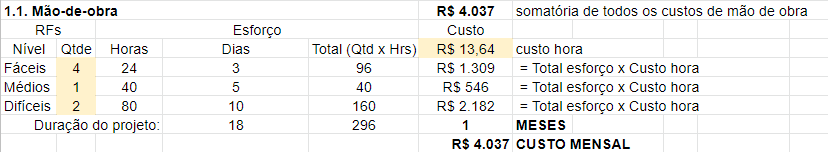
\includegraphics[width=1\textwidth]{images/Mao-de-obra.png}

                \label{fig:maodeobra}
                \centering
                \footnotesize Fonte: Elaborado pelos autores.
            \end{figure}
   \begin{itemize}
      \item Custo-base: R\$ 8.000,00 
        \item Dias-base: 22 | Dia-hora: 8
         \item Custo-hora R\$ 45,45
   \end{itemize} 

           

        % \subsection{Destino dos Custos}

        %     Considerando as funcionalidades do projeto e o número de colaboradores, foram distribuídas tarefas para contabilizar as horas do projeto.

        %     \begin{table*}[h]
        %         % \centering

        %         \resizebox{\columnwidth}{80}{%
        %         \begin{tabular}{|lrrr|r|}
        %             \hline
        %             \multicolumn{1}{|l|}{Funcionalidade}                & \multicolumn{1}{r|}{Dias de Trabalho}
        %                 & \multicolumn{1}{r|}{Membros Atuando}
        %                 & \multicolumn{1}{r|}{Horas Totais}
        %                 &  Custo \\ \hline
        %             \multicolumn{1}{|l|}{Módulo de autenticação}
        %                 & \multicolumn{1}{r|}{3}
        %                 & \multicolumn{1}{r|}{2}
        %                 & \multicolumn{1}{r|}{48} 
        %                 & R\$ 654,55  \\ \hline
        %             \multicolumn{1}{|l|}{Agendamento online}           & \multicolumn{1}{r|}{3}
        %                 & \multicolumn{1}{r|}{2}
        %                 & \multicolumn{1}{r|}{48} 
        %                 & R\$ 654,55  \\ \hline
        %             \multicolumn{1}{|l|}{Prontuário clínico digital}
        %                 & \multicolumn{1}{r|}{10}
        %                 & \multicolumn{1}{r|}{6}
        %                 & \multicolumn{1}{r|}{480} 
        %                 & R\$ 6.545,45  \\ \hline
        %              \multicolumn{1}{|l|}{Registro de alterações assinadas digitalmente}
        %                 & \multicolumn{1}{r|}{10}
        %                 & \multicolumn{1}{r|}{3}
        %                 & \multicolumn{1}{r|}{240} 
        %                 & R\$ 3.272,73  \\ \hline
        %             \multicolumn{1}{|l|}{Gerenciamento de medicação}
        %                 & \multicolumn{1}{r|}{5}
        %                 & \multicolumn{1}{r|}{3}
        %                 & \multicolumn{1}{r|}{120} 
        %                 & R\$ 1.636,36  \\ \hline
        %             \multicolumn{1}{|l|}{Mapeamento Genealógico}
        %                 & \multicolumn{1}{r|}{3}
        %                 & \multicolumn{1}{r|}{3}
        %                 & \multicolumn{1}{r|}{72} 
        %                 & R\$ 981,82  \\ \hline
        %             \multicolumn{1}{|l|}{Controle de vacinação}
        %                 & \multicolumn{1}{r|}{3}
        %                 & \multicolumn{1}{r|}{3}
        %                 & \multicolumn{1}{r|}{72} 
        %                 & R\$ 981,82  \\ \hline
        %             \multicolumn{3}{|l|}{Total}
        %                 & \multicolumn{1}{r|}{1080}
        %                 & R\$ 14.727,27     \\ \hline
        %         \end{tabular}%
        %         }
        %         \caption{Destinação dos custos de desenvolvimento}
        %         \label{tab:custos_func}
        %     \end{table*}

        \subsection{Custos de Operação}

            Após o período de desenvolvimento, os custos para manter o projeto se devem exclusivamente à mensalidade dos servidores e da remuneração do Team Member responsável. Os custos totais podem ser observado na Tabela \ref{tab:custos-maodeobra}.


            \begin{table*}[ht]
            \caption{Custos Totais Estimados}
    \resizebox{\columnwidth}{!}{%
    \begin{tabular}{|lrrrr|r|}
        \hline
        \multicolumn{1}{|l|}{Custo}                              & \multicolumn{1}{r|}{USD}   & \multicolumn{1}{r|}{Câmbio} & \multicolumn{1}{r|}{R\$}       & Quantidade & Total                            \\ \hline
        \multicolumn{1}{|l|}{Amazon CloudWatch}                  & \multicolumn{1}{r|}{1,21}  & \multicolumn{1}{r|}{5,50}   & \multicolumn{1}{r|}{6,655}     & 1          & 6,66                            \\ \hline
        \multicolumn{1}{|l|}{Amazon EC2}                         & \multicolumn{1}{r|}{13,44} & \multicolumn{1}{r|}{5,50}   & \multicolumn{1}{r|}{74,592}    & 1          & 74,59                           \\ \hline
        \multicolumn{1}{|l|}{Amazon RDS for MySQL}               & \multicolumn{1}{r|}{34,97} & \multicolumn{1}{r|}{5,50}   & \multicolumn{1}{r|}{192,335}   & 1          & 192,34                          \\ \hline
        \multicolumn{1}{|l|}{Amazon Simple Storage Service (S3)} & \multicolumn{1}{r|}{0,09}  & \multicolumn{1}{r|}{5,50}   & \multicolumn{1}{r|}{0,495}     & 1          & 0,50                            \\ \hline
        \multicolumn{1}{|l|}{Elastic Load Balancing}             & \multicolumn{1}{r|}{30,32} & \multicolumn{1}{r|}{5,50}   & \multicolumn{1}{r|}{166,76}    & 1          & 166,76                           \\ \hline
        \multicolumn{1}{|l|}{Team Member}                        & \multicolumn{1}{r|}{}      & \multicolumn{1}{r|}{}       & \multicolumn{1}{r|}{8.000,00}  & 1          & 8.000,00                        \\ \hline
        \multicolumn{5}{|l|}{Total Mensal}                                                                                                                                & 8.440,85                       \\ \hline
        \multicolumn{5}{|l|}{Total Anual}                                                                                                                                 & \multicolumn{1}{l|}{101.290,20} \\ \hline
    \end{tabular}%
    }

\label{tab:custos1}
\centering
\footnotesize Fonte: Elaborado pelos autores.
\end{table*}  

        \subsection{Receitas}
            \begin{table}[H]
            \caption{Captação de Recursos}
                \resizebox{\columnwidth}{!}{%
                \begin{tabular}{| p{5cm}|l|l|l|}
                    \hline
                    \multicolumn{1}{|c|}{} & \multicolumn{1}{|c|}{\textbf{Plano Básico  R\$110,00/mês}}  & \multicolumn{1}{c|}{\textbf{Plano Premium  R\$ 165,00/mês}} \\ \hline
                    Agenda  &x &x \\ \hline

                    Prontuário Clínico   &x &x\\ \hline

                    Controle de Vacinação &x &x \\ \hline

                    Gerenciador de Medicamentos &x &x \\ \hline

                    Rastreio de Alterações &   &x  \\ \hline

                    Histórico de Aspectos Hereditários &  &x \\ \hline
                \end{tabular}%
                }

            \label{tab:custos2}
            \centering
            \footnotesize Fonte: Elaborado pelos autores.
            \end{table}

            % \begin{figure}[H]
            %     \centering
            %     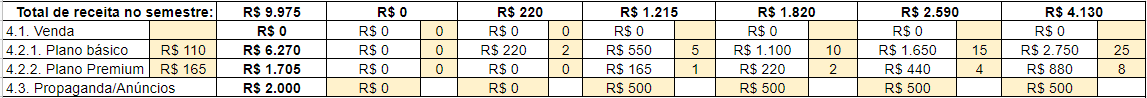
\includegraphics[width=1 \textwidth]{images/REALISTA.png}
            %     \caption{Cenário Realista}
            %     \label{fig:cenariorealista1}
            % \end{figure}
            % \begin{figure}[H]
            %     \centering
            %     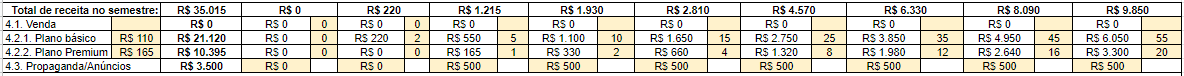
\includegraphics[width=1 \textwidth]{images/REALISA2.png}
            %     \caption{Versão Final do Cenário Realista}
            %     \label{fig:cenariorealista2}
            % \end{figure}

        \subsection{Gráficos dos Cenários}

            % Cenário Realista
            \begin{figure}[H]
                \centering
                 \caption{Primeira Versão do Cenário Realista}
                \includegraphics[width=1 \textwidth]{images/CenárioRealista.png}

                \label{fig:cenariorealistaGrafico1}
                \centering
            \footnotesize Fonte: Elaborado pelos autores.
            \end{figure}

            \begin{figure}[H]
                \centering
                \caption{Segunda Versão do Cenário Realista}
                \includegraphics[width=1 \textwidth]{images/CenárioRealista2.png}

                \label{fig:cenariorealistaGrafico2}
                \centering
            \footnotesize Fonte: Elaborado pelos autores.
            \end{figure}

            \begin{figure}[H]
                \centering
                \caption{Versão Final do Cenário Realista}
                \includegraphics[width=1 \textwidth]{images/CenárioRealista3.png}

                \label{fig:cenariorealistaGrafico3}
                \centering
            \footnotesize Fonte: Elaborado pelos autores.
            \end{figure}

            
            % Cenário Pessimista
            \begin{figure}[H]
                \centering
                \caption{Primeira Versão do Cenário Pessimista}
                \includegraphics[width=1 \textwidth]{images/CenárioPessimista.png}

                \label{fig:cenarioPessimistaGrafico}
                \centering
            \footnotesize Fonte: Elaborado pelos autores.
            \end{figure}

            \begin{figure}[H]
                \centering
                \caption{Versão Final do Cenário Pessimista}
                \includegraphics[width=1 \textwidth]{images/CenárioPessimista2.png}

                \label{fig:cenarioPessimistaGrafico1}
                \centering
            \footnotesize Fonte: Elaborado pelos autores.
            \end{figure}

            % Cenário Otimista
            \begin{figure}[H]
                \centering
                \caption{Primeira Versão do Cenário Otimista}
                \includegraphics[width=1 \textwidth]{images/CenárioOtimista.png}

                \label{fig:cenarioOtimistaGrafico}
                \centering
            \footnotesize Fonte: Elaborado pelos autores.
            \end{figure}

            
            \begin{figure}[H]
                \centering
                 \caption{Versão Final do Cenário Otimista}
                \includegraphics[width=1 \textwidth]{images/CenárioOtimista2.png}

                \label{fig:cenarioOtimistaGrafico2}
                \centering
            \footnotesize Fonte: Elaborado pelos autores.
            \end{figure}

    \section{Fases de entrega}

        O desenvolvimento do projeto foi dividido em três fases de entregas recorrentes, de forma que atendesse à demanda recebida por parte dos clientes. A primeira delas consiste na POC, a segunda a apresentação do MVP e, para finalizar, a Entrega Final. O Quadro \ref{tab:escopo} relaciona as principais funcionalidades da CertVet com a fase em que a sua implementação é esperada.

            \begin{quadro}[H]
                \centering
                \caption{Escopo do Projeto}
                \resizebox{\columnwidth}{!}{%
                \begin{tabular}{|lrrrr|r|}
                    \hline
                    \multicolumn{1}{|l|}{Funcionalidades}                              & \multicolumn{1}{r|}{POC}   & \multicolumn{1}{r|}{MVP} & \multicolumn{1}{r|}{Produto Final}                                   \\ \hline\multicolumn{1}{|l|}{Processo de login}                  & \multicolumn{1}{c|}{X}  & \multicolumn{1}{c|}{X}   & \multicolumn{1}{c|}{X}                                 \\ \hline
                    \multicolumn{1}{|l|}{Módulo de autenticação}                  & \multicolumn{1}{c|}{}  & \multicolumn{1}{c|}{X}   & \multicolumn{1}{c|}{X}                                 \\ \hline
                    \multicolumn{1}{|l|}{Agendamento online}                         & \multicolumn{1}{c|}{} & \multicolumn{1}{c|}{X}   & \multicolumn{1}{c|}{X}                               \\ \hline
                    \multicolumn{1}{|l|}{Prontuário clínico digital}               & \multicolumn{1}{r|}{} & \multicolumn{1}{c|}{X}   & \multicolumn{1}{c|}{X}                             \\ \hline
                    \multicolumn{1}{|l|}{Registro de alterações assinados digitalmente} & \multicolumn{1}{r|}{}  & \multicolumn{1}{r|}{}   & \multicolumn{1}{c|}{X}                                 \\ \hline
                    \multicolumn{1}{|l|}{Gerenciamento de medicação}             & \multicolumn{1}{r|}{} & \multicolumn{1}{r|}{}   & \multicolumn{1}{c|}{X}                               \\ \hline
                    \multicolumn{1}{|l|}{Histórico de aspectos hereditários}                      & \multicolumn{1}{r|}{}      & \multicolumn{1}{r|}{}       & \multicolumn{1}{c|}{X}                           \\ \hline
                    \multicolumn{1}{|l|}{Controle de vacinação}                       & \multicolumn{1}{r|}{}      & \multicolumn{1}{r|}{}       & \multicolumn{1}{c|}{X}                           \\ \hline                  
                \end{tabular}%
                }

            \label{tab:escopo}
            \centering
            \footnotesize Fonte: Elaborado pelos autores.
            \end{quadro}

        \subsubsection{Prova de Conceito}

            A Prova de Conceito, POC, consiste na comprovação de viabilidade técnica da arquitetura proposta, sem considerar implementação de lógica de negócios. Oferece ao cliente uma demonstração de que o produto pode ser desenvolvido, visualizando uma a ideia abstrata de como a aplicação se comporta. 

            Para a POC da CertVet, a equipe apresentou o desenho da arquitetura com as especificações propostas sendo um processo de cadastro de usuário e \emph{login} e regras de negócio simples implementadas no \emph{back-end}. Este processo teve a finalidade de demonstrar o trânsito dos dados através de chamadas com sucesso à API implementada no servidor com respostas previamente esperadas, demonstrando a comunicação entre as camadas foi realizada com sucesso.

        \subsubsection{Produto Mínimo Viável}

            O MVP entregue na segunda fase consiste em uma primeira versão da aplicação com as funcionalidades essenciais identificadas pela análise do grupo junto à profissional devidamente habilitada e praticante.

            Após a liberação do MVP, será possível adicionar novas funcionalidades a partir do \emph{feedbacks} dos usuários e implementação de funcionalidades previamente planejadas.

            A CertVet contempla em seu MVP, além dos processos de cadastro e login, a melhoria do módulo de autenticação do usuário, o serviço de agendamento \emph{on-line} e a criação e manutenção de prontuário clínico digital.

        \subsubsection{Produto Final}

            A partir da finalização do MVP, torna-se possível adicionar as funcionalidades de registro de alterações assinados digitalmente pelo veterinário, gerenciamento de medicação controlada, permitir consultar aspectos hereditários dos animais, controle de vacinação e validação de autenticidade de documento do veterinário junto ao órgão de classe.



    \section{Escolhas e Descartes}
    Desde o início do curso, os alunos são, gradativamente, colocados de forma mais imersiva em situações que simulam os desafios de desenvolver um projeto real. Partindo dos conhecimentos adquiridos com o decorrer dos semestres, ainda na fase inicial do planejamento do projeto, desde a análise e definição do escopo do mesmo, a equipe sabia que seria necessário ter a capacidade de identificar quando mudanças no escopo do projeto se fizessem necessárias, a fim de minimizar retrabalhos e, consequentemente, evitar possíveis atrasos, considerando-se a ampla quantidade de informações a serem levantadas e as tecnologias e ferramentas a serem selecionadas para o desenvolvimento. No entanto, problemas no escopo são quase inevitáveis, portanto, abaixo são discorridas as alterações que se fizeram necessárias durante o desenvolvimento da CertVet.

    A CertVet foi apresentada anteriormente como Sidekick, tal nome surgiu pelo seu significado na língua portuguesa, parceiro de um super-herói, criando uma metáfora sobre a aplicação servir de parceiro para o profissional veterinário. No entanto, em uma das apresentações aos nossos clientes, houve o questionamento sobre o nome não deixar transparente o escopo ao qual pretende cobrir, tendo em vista que a maioria das soluções disponíveis no mercado hoje, possuem o prefixo vet de veterinário na composição de seu nome, como pode ser observado na tabela de Análise Comparativa \ref{tab:comparativa}. Portanto, por estratégia de mercado, a equipe optou por renomear a aplicação para CertVet, somando o prefixo Cert de certificado, considerando sua funcionalidade única dentre as disponíveis de agregar caráter legal às documentações com alterações rastreáveis para verificação do CFMV e CRMV, com o prefixo Vet de veterinário.

    Já no que se refere à infraestrutura, a equipe decidiu retornar à configuração de um \emph{container} por máquina, tendo em vista que a tentativa de utilizar uma máquina comum a dois \emph{containers}, um para o \emph{front-end} e outro para o \emph{back-end}, gerou alguns erros na integração entre ambas as partes, como a desorganização sobre o destino ao qual uma requisição deveria ser repassada. A solução ideal encontrada é a de implementar via serviços Amazon ECS \citeonline{ecs}, que permite execução e manutenção simultânea do número especificado de instâncias, no entanto, a equipe optou prorrogar a implementação desses serviços para o próximo semestre, tendo em vista que a mesma não possui domínio suficiente dessa tecnologia para que a implementação seja efetuada, testada e assegurada dentro do prazo de entrega do MVP, portanto, para garantir o funcionamento acurado da aplicação e cumprir com o prazo anteriormente estipulado, a configuração voltará a ser de um \emph{container} por máquina.

    Por fim, duas novas integrações no \emph{Front-end} foram necessárias para que o funcionamento da aplicação alcançasse o alto nível de experiência do usuário pretendido pela equipe. A integração com a API pública dos \citeonline{correiosCWS}, desenvolvida em REST e que utiliza o protocolo HTTP, tornou possível que os dados do endereço do usuário fossem recuperados a partir do CEP informado. \citeonline{correiosAPI}. Enquanto a API do \citeonline{ibgeAPI}, também de caráter público, permite a listagem de todas as unidades federativas do território brasileiro.
    O esquema após a integração com a API dos Correios e API do IBGE estão ilustrados na Figura \ref{fig:infra3}, no entanto, a versão inicial da arquitetura do sistema pode ser visto mais detalhadamente na Figura \ref{fig:infra}.

    \begin{figure}[H]
        	\centering
            \caption{Versão anterior do esquema de Infrastrutura}

        	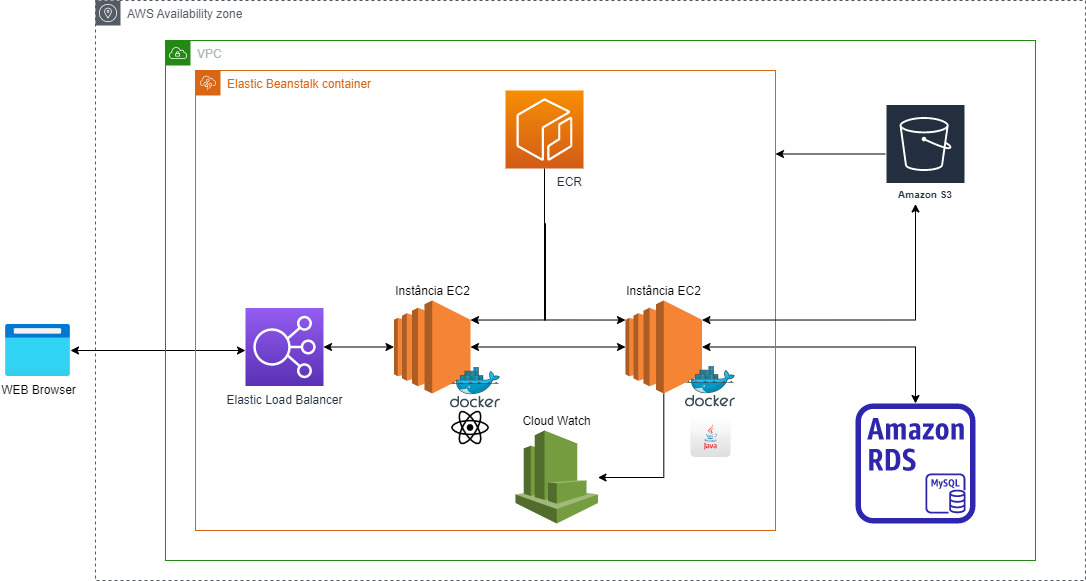
\includegraphics[width=0.9\textwidth]{ArquiteturaAplicacao.png}
        	\label{fig:infra}

        	\centering
            {\footnotesize Fonte: Elaborado pelos autores.}
   \end{figure}
\DIFaddbegin 

    \DIFadd{Após o }\emph{\DIFadd{feedback}} \DIFadd{dos professores na última avaliação, o grupo entendeu a necessidade de mudar o conceito de modelos para usuários e de tabelas para a aplicação.
}

    \DIFadd{A abordagem proposta altera a forma de gerir os acessos dos usuários e de esclarecer o relacionamento de procedimentos da clínica.
}

    \DIFadd{Durante os meses de Dezembro e Janeiro, a aplicação foi atualizada para que os possíveis problemas de desenvolvimento enfrentados anteriormente conseguissem ser evitados, bem como atualizando as funcionalidades que já existiam.
}

    \DIFadd{Utilizando o modelo que a especificação do pacote }\emph{\DIFadd{Spring Security}} \DIFadd{oferece para controle de permissões de acesso, implementou-se o modelo de controle de acessos a recursos do sistema determinados por autoridade. Como efeito, a CertVet passa a compreender diferentes perfis de usuário gerenciados pelo usuário administrador da clínica.
}

    \DIFadd{Verificou-se que simplificar a forma de controle dos perfis básicos permite a criação de acessos mais flexíveis de acordo com necessidades pontuais que podem ser identificadas de acordo com a regra de negócios do cliente, sem alterar o funcionamento da aplicação e melhorando a experiência de desenvolvimento.
}

    \DIFadd{Devido a complexidade dos procedimentos aplicados durante o atendimento dos animais, entendeu-se necessário refinar as entidades que interagem com o prontuário, sendo expandidas as entidades Exame, Procedimento e Cirurgia.
}

    \DIFadd{Para a entidade de controle de estoque, o conceito do modelo tem objetivo de controlar os movimentos de entrada e saída de produtos, realizando o somatório de quantidades para apresentação de saldo.
}

    \DIFadd{As representações do MER e DER  estão ilustradas, respectivamente, pela Figura \ref{fig:MER2} e Figura \ref{fig:DER2}, no entanto as versões iniciais podem ser vistas na Figura \ref{fig:MER} e Figura \ref{fig:DER}.
}

    \begin{figure}[H]
        \centering
        \caption{\DIFaddFL{Versão anterior do Modelo Entidade Relacionamento}}
        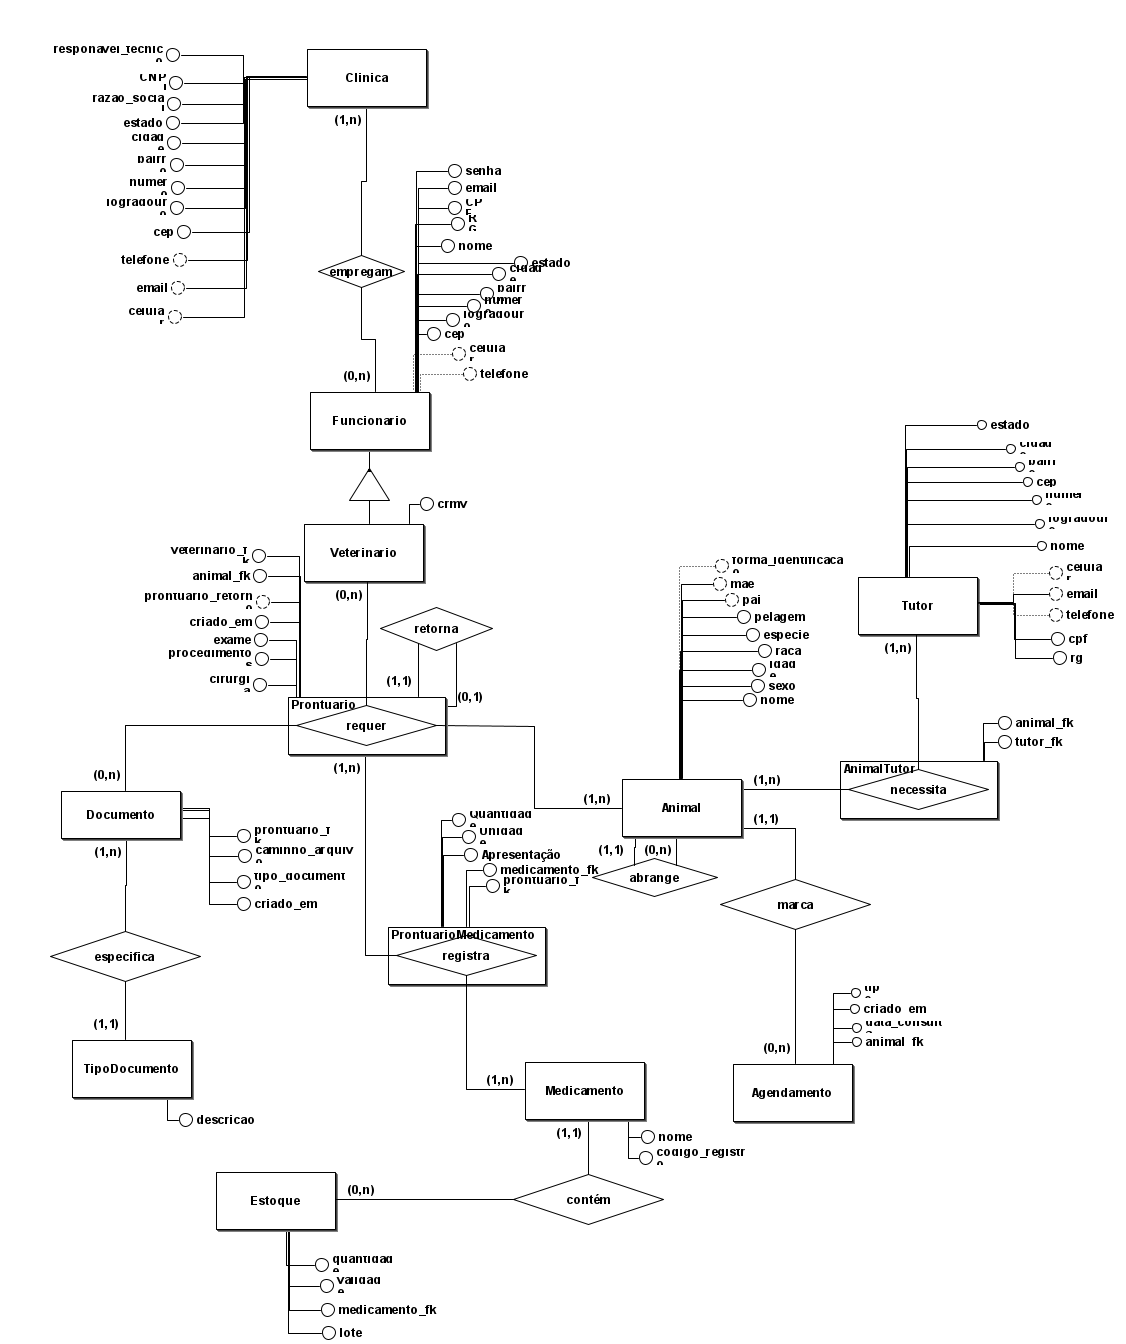
\includegraphics[ width=\linewidth]{images/ProjetoPI1.2 .png}

        \label{fig:MER}
        \centering
        {\footnotesize \DIFaddFL{Fonte: Elaborado pelos autores.}}
    \end{figure}

    \begin{figure}[H]
        \centering
        \caption{\DIFaddFL{Versão anterior do Diagrama Entidade-Relacionamento}}
        \includegraphics[width=0.7\textwidth]{images/Modelo Lógico.png}

        \label{fig:DER}
        \centering
        {\footnotesize \DIFaddFL{Fonte: Elaborado pelos autores.}}
    \end{figure}

    \DIFadd{O time adotou o padrão }\emph{\DIFadd{Data Transfer Object}} \DIFadd{(DTO), que possui o transporte de dados dentro da aplicação como única função, ainda no início da implementação da aplicação, no entanto ao seguir esse padrão não deve-se possuir métodos que alterem seus valores como os métodos }\emph{\DIFadd{Setters}}\DIFadd{, logo, a viabilidade de uso da classe }\emph{\DIFadd{Record}} \DIFadd{se tornou objeto de estudo do time, tendo em vista que os }\emph{\DIFadd{Records}} \DIFadd{são serializáveis e podem substituir os DTOs usados dentro da aplicação, buscando a imutabilidade das classes e a diminuição de escrita no código. No entanto, ressalta-se nesse ponto que a utilização dessa classe ainda está em análise.
}\DIFaddend 


\section{Métricas}

    Foram geradas diferentes métricas para acompanhar o desenvolvimento do projeto, porém, devido a dificuldades enfrentadas pelos membros, as métricas não correspondem fielmente a contribuição de cada um dos envolvidos. Alguns integrantes encontraram barreiras em subir sua contribuição nos diferentes meios de controle de versionamento, como SVN e GitHub, e o trabalho foi repassado para que outro integrante fizesse o \emph{upload} do arquivo gerado.
    Tais barreiras prejudicaram a geração das métricas adequadas, e nota-se que muitos \emph{uploads} e \emph{commits} aparecem como picos após longos períodos de inatividade, porém a equipe trabalhou de forma contínua, durante as semanas que se desenvolveu o projeto. 

    Outro ponto de atenção é com relação ao período utilizado para gerar as métricas do GitStats, pois ele conta a partir das últimas 32 semanas, sendo que, até o momento de gerar as estatísticas, o projeto desenvolveu-se nas últimas 14 semanas.

    \subsection{GitStats}

    O Github foi o meio que a equipe encontrou de compartilhar seu progresso no projeto, por ser um serviço que todos estavam familiarizados. Apesar disso, cada integrante fazia seu upload de forma diferente, alguns fazendo o commit diretamente na interface do navegador, enquanto outros atualizavam seus commits utilizando a função pull request (principalmente na parte de desenvolver o código do sistema). Essa diferença entre formas de subir os dados na plataforma GitHub influenciou os resultados estatísticos obtidos com o GitStats. Nota-se que apesar de alguns integrantes desenvolverem muitas linhas de códigos, por serem dentro de um mesmo commit, isso reduziu a porcentagem calculada de contribuição dos integrantes em questão. 

    Novamente, deve-se observar que o \emph{pair programming} feito em sala de aula, onde os integrantes criavam o código juntos, porém apenas um logado no sistema e enviando as linhas produzidas, interferiu no resultado das métricas, o que omitiu a participação de todos os integrantes envolvidos.

    Foram geradas métricas utilizando o GitStats para 3 diferentes repositórios, que levaram em conta a divisão macro do projeto: Documentos (todos os textos feitos pelos integrantes em LaTeX, no documento compartilhado no Overleaf, assim como as propostas iniciais e apresentações), \emph{front-end} (todos os \emph{commits} de códigos referentes ao\emph{front-end} tanto da POC, como do MVP) e \emph{back-end} (todos os \emph{commits} de códigos referentes ao \emph{back-end} tanto da POC, como do MVP).


    \subsubsection{GitStats do Repositório Documentos}

    Neste repositório foram adicionados todo o desenvolvimento textual do projeto, assim como os slides das apresentações, propostas iniciais e foi o primeiro repositório da equipe a ser criado. 

    No gráfico presente na Figura \ref{fig:semanas contadas}, é possível ver que as atividades iniciam-se de acordo com o semestre corrente, contando retrospectivamente a partir da geração da métrica em 20 de Novembro de 2022, conforme observado na Figura \ref{fig:geralDoc}.

    \begin{figure}[H]
            \centering
            \caption{Visão Geral do Documento - GitHub.}
            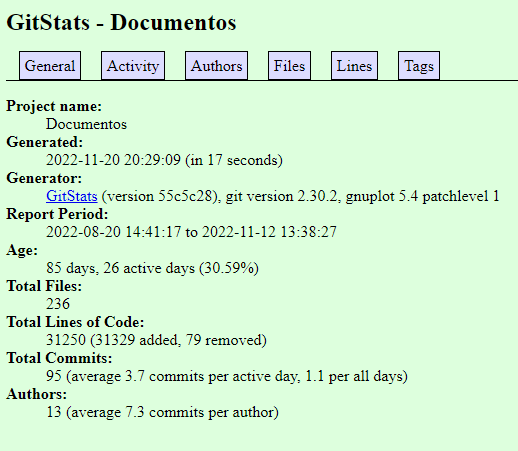
\includegraphics[width=1 \textwidth]{Gitstats/documento/geralDoc.png}
            {\footnotesize Fonte: Elaborado pelos autores.}
            \label{fig:geralDoc}
    \end{figure}


    \begin{figure}[H]
            \centering
            \caption{Gráfico das Semanas Contadas}
            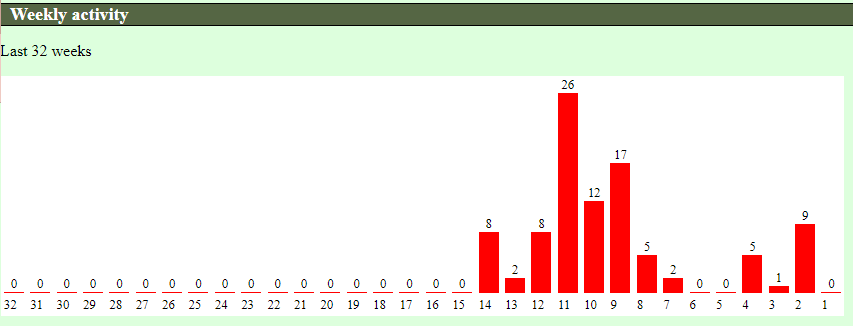
\includegraphics[width=1 \textwidth]{Gitstats/documento/semanas contadas.png}
            \label{fig:semanas contadas}
            \centering

        \footnotesize Fonte: Elaborado pelos autores.
    \end{figure}

    \begin{figure}[H]
            \centering
            \caption{Gráfico dos Dias da Semana}
            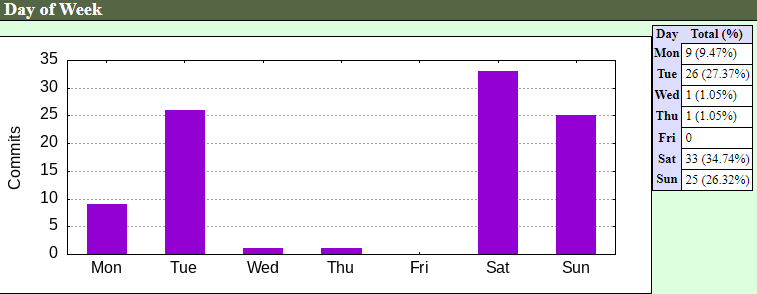
\includegraphics[width=1 \textwidth]{Gitstats/documento/dias da semana.png}

            \label{fig:diadasemana}
            \centering
            \footnotesize Fonte: Elaborado pelos autores.
    \end{figure} 

    No gráfico presente na Figura \ref{fig:diadasemana} nota-se o padrão de desenvolvimento coincidindo com os dias reuniões, indo de sábado até terça. A queda nos \emph{commits} de quarta a sexta é justificada pelo fato dos integrantes cursarem outras matérias no curso, que também demandam dedicação.

      \begin{figure}[H]
            \centering
            \caption{Gráfico das Horas do Dia.}
            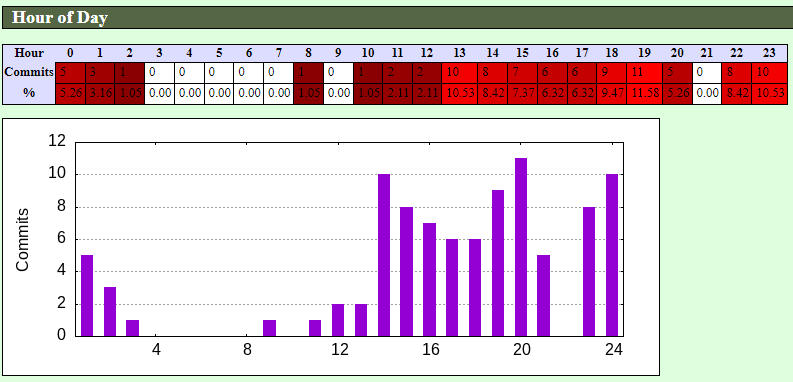
\includegraphics[width=1 \textwidth]{Gitstats/documento/horasdodia.png}
            {\footnotesize Fonte: Elaborado pelos autores.}
            \label{fig:horadodia}
        \end{figure} 

    Com relação aos autores dos \emph{commits}, nota-se que os integrantes aparecem duplicados na Figura \ref{fig:listaautores}. Essa repetição se dá por causa da forma de envio dos dados. Na Figura \ref{fig:dominio} é possível ver os diferentes domínios utilizados pelos autores, que impactou o resultado. O gráfico de commits por autor encontra-se na Figura \ref{fig:commitautor}

    \begin{figure}[H]
                \centering
                \caption{Lista de Autores.}
                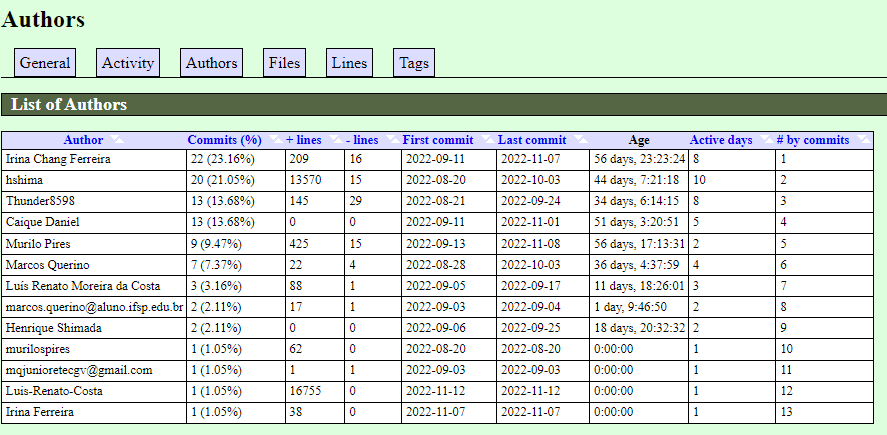
\includegraphics[width=1 \textwidth]{Gitstats/documento/lista de autores.png}
                {\footnotesize Fonte: Elaborado pelos autores.}
                \label{fig:listaautores}
            \end{figure}

    \begin{figure}[H]
            \centering
            \caption{Domínio Utilizado pelos Autores.}
            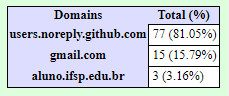
\includegraphics[scale = 1.5]{Gitstats/documento/dominios1.png}

            {\footnotesize Fonte: Elaborado pelos autores.}
            \label{fig:dominio}
        \end{figure}  


    \begin{figure}[H]
            \centering
            \caption{Gráfico de \emph{Commits} por Autor.}
            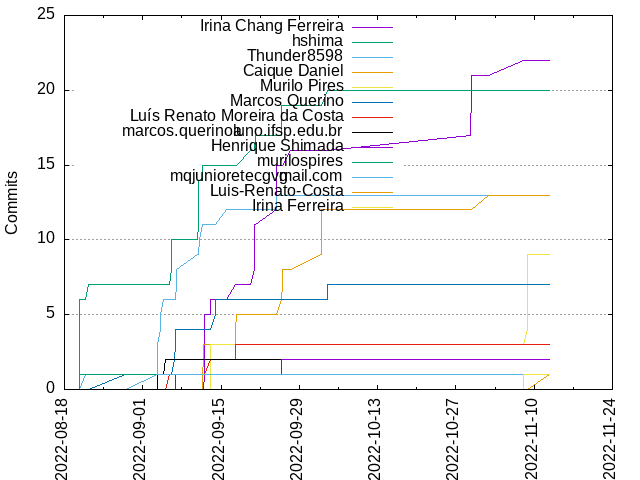
\includegraphics[width=1 \textwidth]{Gitstats/documento/commitsPorAuthor.png}
            {\footnotesize Fonte: Elaborado pelos autores.}
            \label{fig:commitautor}
    \end{figure} 



\subsubsection{GitStats do Repositório do \emph{Front-end}}
    Nas Figuras \ref{fig:geralFront}, \ref{fig:semanasFront}, \ref{fig:diasemanaFront}, \ref{fig:horasFront}, \ref{fig:autorFront}, \ref{fig:commitFront} e \ref{fig:extensaoFront} são expostas as métricas geradas no repositório \emph{Front-end}.

        \begin{figure}[H]
                \centering
                \caption{Visão Geral do Front-end} - GitHub.
                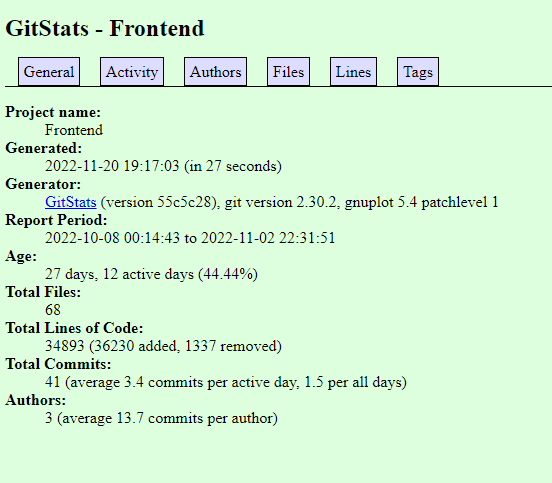
\includegraphics[width=1 \textwidth]{Gitstats/front-end/geralFront.png}
                {\footnotesize Fonte: Elaborado pelos autores.}
                \label{fig:geralFront}
        \end{figure}     

        \begin{figure}[H]
                \centering
                \caption{Gráfico de Semanas Contadas.}
                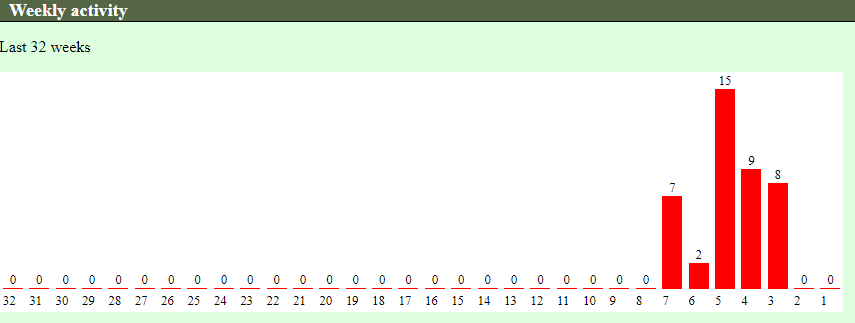
\includegraphics[width=1 \textwidth]{Gitstats/front-end/SemanasFront.png}
                {\footnotesize Fonte: Elaborado pelos autores.}
                \label{fig:semanasFront}
        \end{figure}    

        \begin{figure}[H]
                \centering
                \caption{Gráfico de Dias da Semana do  Front-end.}
                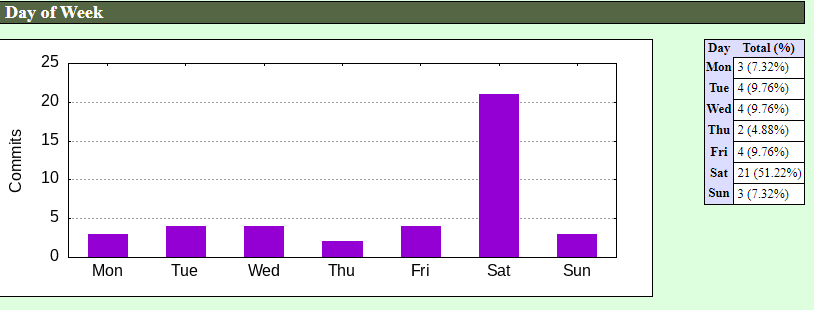
\includegraphics[width=1 \textwidth]{Gitstats/front-end/DiasdaSemana.png}
                {\footnotesize Fonte: Elaborado pelos autores.}
                \label{fig:diasemanaFront}
        \end{figure}  

        \begin{figure}[H]
                \centering
                \caption{Gráfico de Horas por Dia do Front-end.}
                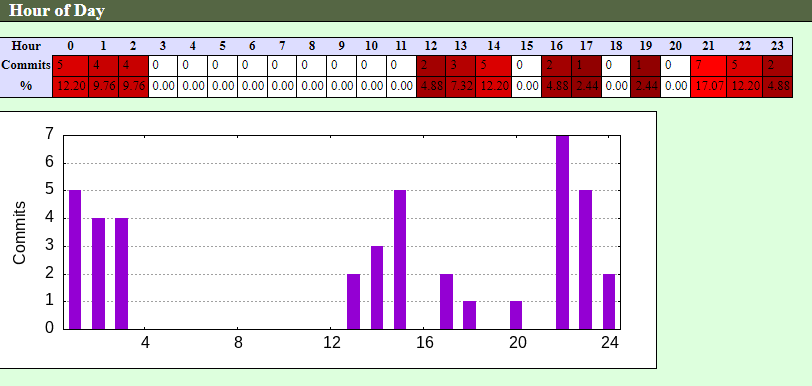
\includegraphics[width=1 \textwidth]{Gitstats/front-end/HorasdoDia.png}
                {\footnotesize Fonte: Elaborado pelos autores.}
                \label{fig:horasFront}
        \end{figure} 

        \begin{figure}[H]
                \centering
                \caption{Lista de Autores do
                Front-end.}
                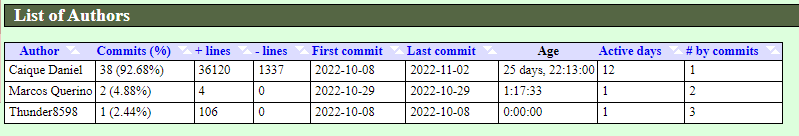
\includegraphics[width=1 \textwidth]{Gitstats/front-end/ListaAutores.png}
                {\footnotesize Fonte: Elaborado pelos autores.}
                \label{fig:autorFront}
        \end{figure}   

        \begin{figure}[H]
                \centering
                \caption{Gráfico de Commits por Autor.}
                \includegraphics[width=1 \textwidth]{Gitstats/front-end/CommitsPorAutor.png}
                {\footnotesize Fonte: Elaborado pelos autores.}
                \label{fig:commitFront}
        \end{figure}   

        \begin{figure}[H]
                \centering
                \caption{Extensões utilizadas no \emph{Front-end}.}
                \includegraphics[scale = 1.2]{Gitstats/front-end/ListadeExtensoes.png}

                {\footnotesize Fonte: Elaborado pelos autores.}
                \label{fig:extensaoFront}
        \end{figure}  



        \subsubsection{GitStats do Repositório \emph{back-end}}

        Neste repositório houve alguns erros na geração de dados coerentes. Devido o repositório encontrar-se como privado, os dados não estavam sendo gerados. Após tornarmos o mesmo para público, foi possível gerar as métricas, mas elas foram contabilizadas como um único dia. Não conseguimos descobrir a causa dessa incoerência de resultados. 
        Pode-se conferir os resultados gerados na sequência de Figuras \ref{fig:geralBack}, \ref{fig:semanasBack}, \ref{fig:diasBack}, \ref{fig:HorasBack}, \ref{fig:AutorBack}, \ref{fig:commitBack} e \ref{fig:extensoesBack}.

            \begin{figure}[H]
                \centering
                \caption{Visão Geral do \emph{back-end} - GitHub.}
                \includegraphics[width=1 \textwidth]{Gitstats/back-end/GeralBack.png}
                {\footnotesize Fonte: Elaborado pelos autores.}
                \label{fig:geralBack}
            \end{figure} 


            \begin{figure}[H]
                \centering
                \caption{Gráfico de Semanas Contadas.}
                \includegraphics[width=1 \textwidth]{Gitstats/back-end/SemanasBack.png}
                {\footnotesize Fonte: Elaborado pelos autores.}
                \label{fig:semanasBack}
            \end{figure}   

            \begin{figure}[H]
                \centering
                \caption{Gráfico de Dias da Semana do \emph{back-end}.}
                \includegraphics[width=1 \textwidth]{Gitstats/back-end/DiasBack.png}
                {\footnotesize Fonte: Elaborado pelos autores.}
                \label{fig:diasBack}
            \end{figure}

            \begin{figure}[H]
                \centering
                \caption{Gráfico de Horas por Dia do \emph{back-end}.}
                \includegraphics[width=1 \textwidth]{Gitstats/back-end/HorasBack.png}
                {\footnotesize Fonte: Elaborado pelos autores.}
                \label{fig:HorasBack}
            \end{figure} 

            \begin{figure}[H]
                \centering
                \caption{Lista de Autores do \emph{back-end}.}
                \includegraphics[width=1 \textwidth]{Gitstats/back-end/AutorBack.png}
                {\footnotesize Fonte: Elaborado pelos autores.}
                \label{fig:AutorBack}
            \end{figure}

            \begin{figure}[H]
                \centering
                \caption{Gráfico de Commits por Autor.}
                \includegraphics[width=1 \textwidth]{Gitstats/back-end/commitsAutorBack.png}
                {\footnotesize Fonte: Elaborado pelos autores.}
                \label{fig:commitBack}
            \end{figure}    

            \begin{figure}[H]
                \centering
                \caption{Lista de Extensões Utilizadas no \emph{back-end}.}
                \includegraphics[scale = 1.2]{Gitstats/back-end/extensoesBack.png}

                {\footnotesize Fonte: Elaborado pelos autores.}
                \label{fig:extensoesBack}
            \end{figure}  


    \subsection{StatSVN}

        O Subversion, ou SVN foi utilizado para controlar as entregas feitas pela equipe aos professores. Ressaltamos que apenas 3 integrantes conseguiram efetivamente realizar as entregas por esse sistema, o que gerou um resultado não fidedigno da realidade, visto que todos os integrantes participaram do desenvolvimento. 

        Nas Figuras \ref{fig:desenvolvimentoSVN}, \ref{fig:linhaCod}, \ref{fig:diaSemana} e \ref{fig:horaDia} são expostas as métricas geradas pelo StatSVN.

    \begin{figure}[H]
                \centering
                \caption{Visão Geral do Desenvolvimento no SVN.}
                \includegraphics[width=1 \textwidth]{StatSVN/StatDesenvolvimento.png}
                {\footnotesize Fonte: Elaborado pelos autores.}
                \label{fig:desenvolvimentoSVN}
            \end{figure}

    \begin{figure}[H]
                \centering
                \caption{Gráfico Referentes as Linhas de Códigos.}
                \includegraphics[width=1 \textwidth]{StatSVN/linha de codigo autor.png}
                {\footnotesize Fonte: Elaborado pelos autores.}
                \label{fig:linhaCod}
            \end{figure}

    \begin{figure}[H]
                \centering
                \caption{Gráfico Referente aos Dia da Semana.}
                \includegraphics[width=1 \textwidth]{StatSVN/DiadaSemana.png}
                {\footnotesize Fonte: Elaborado pelos autores.}
                \label{fig:diaSemana}
            \end{figure} 

    \begin{figure}[H]
                \centering
                \caption{Gráfico Referentes as Horas do Dia.}
                \includegraphics[width=1 \textwidth]{StatSVN/HoradoDia.png}
                {\footnotesize Fonte: Elaborado pelos autores.}
                \label{fig:horaDia}
            \end{figure} 

\section{Testes de Segurança}

    \subsection{Teste de Segurança dos Headers}

    \begin{figure}[H]
        \centering
        \includegraphics[width=1 \textwidth]{images/headers1.jpeg}    \caption{Resultado do Teste de Headers}
        \label{fig:header}
    \end{figure}

    \subsection{Teste de Segurança SSL}
        Além da implementação do TLS, foram adicionadas políticas de segurança através dos Headers das requisições, de forma a instruir o navegador sobre as ações que são permitidas no site.
        Como referência para a verificação de Headers de segurança, foi orientada a utilização do site Security Headers\citeonline{header}.
        Para a configuração dos Headers, foi utilizado como referência os site MDN Web Docs \citeonline{mdn}.


    \subsubsection{ Teste de Segurança Inicial}

    Antes de realizar qualquer tentativa de implementação, foi realizado um teste com a aplicação no estado atual (as is). Posteriormente, para documentar a situação, foi realizada uma nova consulta adicionada ao apêndice, onde obteve-se o seguinte resultado mostrado na Figura \ref{fig:sslFront}

    \begin{figure}[H]
        \centering
        \includegraphics[width=0.9 \textwidth]{images/headerfront.png}
        \caption{Teste SSL da Aplicação}
        \label{fig:sslFront}
    \end{figure}    

    \subsubsection{Teste de Segurança Final}

    Após alguns ajustes e mais estudos sobre os certificados de segurança, obteve-se o seguinte resultado mostrado na Figura \ref{fig:sslFrontfinal} e também no Apêndice \ref{apendiceE}

    \begin{figure}[H]
        \centering
        \includegraphics[width=0.9 \textwidth]{images/sslFront.png}
        \caption{Teste SSL da Aplicação Final}
        \label{fig:sslFrontfinal}
    \end{figure}

%%%%%%%%% TODO ajustar texto de considerações finais %%%%%%%%%%%%%%%%%%%%%%    

\chapter[Conclusão]{Conclusão}

    A acessibilidade de tecnologias em nuvem e emprego de tecnologias portáveis de containerização permitem que aplicações sejam criadas e transportadas com mínimo de interferência para o mantenedor e seus clientes. Entretanto, ao utilizar soluções proprietárias, como o serviço Amazon S3, é necessário considerar o tipo de comprometimento por vendor lock in que corre-se o risco de expor a aplicação.

    Em suma, as utilização e aproveitamento de recursos computacionais, principalmente em nuvem, na área de medicina veterinária faz-se não somente benéfica por eliminar o risco de perda de dados em mídias físicas e aumentar a velocidade de recuperação de dados importantes e sensíveis.

    As normas que regulam as atividades médico-veterinárias, em especial sobre medicação controlada, podem sofrer alterações que nem sempre são acompanhadas pelo técnico no momento em que são publicadas. Uma ferramenta de gestão focada nesta atividade reduz o risco do negócio se enquadrar em uma situação de irregularidade.

\chapter[Links do Projeto]{Links do Projeto}
    % no momento este tópico fica como capitulo, mas na entrega final ele vai virar um tópico do capitulo de métricas
    \begin{figure} [htb!]
        \centering
        \includegraphics[width=0.3\textwidth]{qrcode/qrcode_GIT.png}
        \caption{Link Repositório no GitHub}
        {\footnotesize \url{ https://github.com/orgs/EquipeRocketIFSP/repositories}}
        \label{fig:qrcode_GIT}
    \end{figure}

     \begin{figure}[htb!]
        \centering
        \includegraphics [width=0.3\textwidth]{qrcode/qrcode_YT.png}
        \caption{Link Página no YouTube}
        {\footnotesize \url{https://youtube.com/@equiperocket6085}}
        \label{fig:qrcode_YT}
    \end{figure}

    \begin{figure}[htb!]
        \centering
        \includegraphics[width=0.3\textwidth]{qrcode/qrcode_BLOG.png}
        \caption{Link Página do Blog}
        {\footnotesize \url{https://equipe-rocket-ifsp.blogspot.com}}
        \label{fig:qrcode_BLOG}
    \end{figure}

    \begin{figure}[htb!]
        \centering
        \includegraphics[width=0.3\textwidth]{qrcode/svn.png}
        \caption{Link Repositório da Equipe no SVN}
        {\footnotesize \url{https://svn.spo.ifsp.edu.br/svn/a6pgp/S202202-PI-NOT/Rocket}}
        \label{fig:svn}
    \end{figure}

   
    \begin{figure}[htb!]
         \centering
         \includegraphics[width=0.3\textwidth]{qrcode/qrcode_SITE.png}
         \caption{\emph{Site} CertVet}
         {\footnotesize \url{https://certvet-front.us-east-1.elasticbeanstalk.com}}
         \label{fig:linksite}
    \end{figure}   


\chapter[Considerações Finais]{Considerações Finais}

    A equipe encontrou diversas dificuldades ao longo do projeto, que serviram de aprendizado para a carreira na área da Tecnologia da Informação.
    A organização e distribuição das tarefas provou-se ser a habilidade mais valiosa que uma equipe deve ter, não diminuindo a capacidade intelectual de cada um dos membros. 

    Fatores externos também impediram que a equipe pudesse entregar o projeto idealizado nas primeiras reuniões do curso. O principal impedimento foi a recusa do orgão fiscalizador federal, CFMV, de liberar acesso á sua API, acesso que, caso fosse concedido, permitiria validar o registro do profissional que acessa o sistema, garantindo uma segurança à aplicação e àqueles que a usam. O contato, via Lei de Acesso a informação foi feito em dois emails, que podem ser vistos no Apêndice \ref{apendiceA}  e \ref{apendiceC}. Assim como a resposta do CFMV dada ao primeiro contato, vista no Apêndice \ref{apendiceB}.

    Outro fator externo se deu com relação aos testes de segurança, visto que o serviço de servidor escolhido através da AWS não estava configurado para atender todos os requisitos necessário para atingir a nota mínima exigida pelos professores. Com isso mudamos a entrega desse requisito para a entrega final do documento.


%---
% pós-textual
% ---


\postextual

% quando não esta utilizando biblatex tem que carregar as referencias aqui
\IfPackageLoaded{biblatex}{%
\printbibliography

\ifthenelse{\boolean{utilizarREFINDENT}}{%
}

}{%
\bibliography{referencias,exemplos/abntex2-doc-abnt-6023}
}

%% ----------------------------------------------------------
% Glossário
% ----------------------------------------------------------
%
%
\ifdef{\printnoidxglossary}{
    \addcontentsline{toc}{chapter}{GLOSSÁRIO}
    \printnoidxglossary[style=glossario]
    %\printglossaries
}{}

% ----------------------------------------------------------
% Apêndices
% Documentos gerados pelo próprio autor
% ----------------------------------------------------------

% ---
% Inicia os apêndices
% ---
\begin{apendicesenv}

% Imprime uma página indicando o início dos apêndices
\partapendices

% ----------------------------------------------------------
%\chapter{Quisque libero justo}
% ----------------------------------------------------------

%\preencheComTexto

\begin {appendices}
\chapter{Email de Contato Inicial}



\includegraphics[page=1, width=1\linewidth,height=0.8\textheight]{Apêndices/email1.PNG}

\newpage
\label{apendiceA}
\end{appendices}

\begin {appendices}
\chapter{Email de Resposta CFMV}
\includegraphics[page=1, width=1\linewidth,height=0.8\textheight]{Apêndices/emailresposta.png}

\newpage
\label{apendiceB}
\end{appendices}
\newpage

\begin {appendices}
\chapter{Novo Contato ao CFMV}


\includegraphics[page=1, width=1\linewidth,height=0.8\textheight]{Apêndices/email2.png}

\label{apendiceC}
\end{appendices}

\begin {appendices}
\chapter{Teste de Headers}
\includegraphics[page=1, width=1\linewidth,height=0.8\textheight]{Apêndices/headersfinal.pdf}
\label{apendiceD}
\end{appendices}

\begin {appendices}
\chapter{Teste de SSL}
\includegraphics[page=1, width=1\linewidth,height=0.8\textheight]{Apêndices/sslFront.pdf}
\label{apendiceE}
\end{appendices}

\begin {appendices}
\chapter{Blog da Equipe}
\includegraphics[page=1, width=1\linewidth,height=0.8\textheight]{Apêndices/EquipeRocketBlog.pdf}

\includepdf[pages={2-},scale=0.80,pagecommand={}]{Apêndices/EquipeRocketBlog.pdf}

\end{appendices}








%\newpage
%\chapter{Email de Contato Inicial}
%\begin{figure}
  %%   \includegraphics[width=1\textwidth]{Apêndices/email1.PNG}
 %  \caption{Email de contato inicial.}
 %   \label{email1}
%\end{figure}





%\chapter{Email de Resposta do CFMV}
%\begin{figure}
 %   \centering
  %  \includegraphics[width=1\textwidth]{Apêndices%/emailresposta.png}
   % \caption{Resposta enviada pelo CFMV}
    %\label{resposta}
%\end{figure}



%\chapter{Novo Contato ao CFMV}

%\begin{figure}
 %   \centering
  %  \includegraphics[width=1\textwidth]{Apêndices/email2.png}
   % \caption{Email de contato com as leis}
%    \label{email2}
%\end{figure}
% ----------------------------------------------------------
%\chapter{Nullam elementum urna vel imperdiet sodales elit ipsum pharetra ligula
%ac pretium ante justo a nulla curabitur tristique arcu eu metus}
% ----------------------------------------------------------
%\preencheComTexto
\
%\begin{figure}
  %  \centering
  %  \includegraphics{Apêndices/EquipeRocketBlog.pdf}
   % \caption{Caption}
    %\label{fig:my_label}
%\end{figure}

\end{apendicesenv}
% ---




% ----------------------------------------------------------
% Anexos
% Documentos gerados por outros autores
% ----------------------------------------------------------

% ---
% Inicia os anexos
% ---
\begin{anexosenv}
\anexos

% Imprime uma página indicando o início dos anexos
\partanexos

% ---
% \chapter{Manual todonotes(parcial)}
%\label{manual-todonotes}
% ---
%\index{pdf}
% se pages = "-"  fica com arquivo completo
%\includepdf[pages=1-3,scale=0.8,frame=true,pagecommand={}]{anexos/todonotes.pdf}

% ---
% Para incluir sem gerar a quebra de página inicial no anexo
%-\includepdf[pages=1,scale=0.7,frame=true,pagecommand=\chapter{Manual pdfpages(parcial)}\label{manual-pdfpages}]{anexos/pdfpages.pdf}
%-\includepdf[pages=2-3,scale=0.8,frame=true,pagecommand={}]{anexos/pdfpages.pdf}

% ---
%--\chapter{Manual acronym(parcial)}
%--\index{pdf}
% somente algumas páginas para exemplo sem borda
%--\includepdf[pages=1-3,frame=false,pagecommand={}]{anexos/acronym.pdf}



%\includepdf[frame=true,scale=0.7,pagecommand=\chapter{Referência Rápida %pifont}\label{pifont-quickref}]{anexos/pifont.pdf}


\includepdf[pages=1,scale=0.8,frame=false,pagecommand=\chapter{Atestado Sanitário}\label{atestado sanitario}]{anexos/anexos_pdfs/anexo1.pdf}


\includepdf[pages=1,scale=0.8,frame=false,pagecommand=\chapter{Atestado de Óbito}\label{atestado de obito}]{anexos/anexos_pdfs/anexo2.pdf}

\includepdf[pages=1,scale=0.8,frame=false,pagecommand=\chapter{Termo de Consentimento para Exames}\label{consentimento exame}]{anexos/anexos_pdfs/anexo3.pdf}


\includepdf[pages=1,scale=0.8,frame=false,pagecommand=\chapter{Termo de Consentimento para Procedimento Terapêutico de Risco}\label{consentimento tratamento}]{anexos/anexos_pdfs/anexo4.pdf}

\includepdf[pages=1,scale=0.8,frame=false,pagecommand=\chapter{Termo de Consetimento para Retirada de Corpo}\label{retirar corpo}]{anexos/anexos_pdfs/anexo5.pdf}

\includepdf[pages=1,scale=0.8,frame=false,pagecommand=\chapter{Termo de Consentimento para Procedimento Cirúrgico}\label{consentimento cirurgico}]{anexos/anexos_pdfs/anexo6.pdf}

\includepdf[pages=1,scale=0.8,frame=false,pagecommand=\chapter{Termo de Consentimento para Internação}\label{consentimento internacao}]{anexos/anexos_pdfs/anexo7.pdf}

\includepdf[pages=1,scale=0.8,frame=false,pagecommand=\chapter{Termo de Consentimento para Procedimento Anestésico}\label{consentimento anestesico}]{anexos/anexos_pdfs/anexo8.pdf}

\includepdf[pages=1,scale=0.8,frame=false,pagecommand=\chapter{Termo de Consentimento para Eutanásia}\label{consentimento eutanasia}]{anexos/anexos_pdfs/anexo9.pdf}

\includepdf[pages=1,scale=0.8,frame=false,pagecommand=\chapter{Termo de Consentimento para Retirada Sem Alta Médica}\label{retirada sem alta}]{anexos/anexos_pdfs/anexo10.pdf}

\includepdf[pages=1,scale=0.8,frame=false,pagecommand=\chapter{Atestado de Vacinação}\label{atestado de vacina}]{anexos/anexos_pdfs/anexo11.pdf}

\includepdf[pages=1,scale=0.8,frame=false,pagecommand=\chapter{Termo de Consentimento para Doação de Corpo para Pesquisa}\label{doacao de corpo}]{anexos/anexos_pdfs/anexo12.pdf}


\end{anexosenv}





\end{document}
